\documentclass[11pt]{article}      % Comments after  % are ignored
\usepackage{amsmath,amssymb,amsfonts} % Typical maths resource packages
\usepackage{graphics}                 % Packages to allow inclusion of graphics
\usepackage{color}                    % For creating coloured text and background
\usepackage{hyperref}                 % For creating hyperlinks in cross references
\usepackage{fullpage}
\usepackage{placeins}
\usepackage{ifpdf}
\usepackage{graphicx}
\usepackage{textcomp}
\usepackage{array}
\usepackage[export]{adjustbox}

\newcommand{\HRule}{\rule{\linewidth}{0.5mm}} % Defines a new command for the horizontal lines, change thickness here
%\usepackage{array}
%\newcolumntype{L}[1]{>{\raggedright\let\newline\\\arraybackslash\hspace{0pt}}m{#1}}
\def\HCode#1{}
\def\htmlanchor#1{\HCode{<a id="#1"></a>}}
%\def\hcolwidth#1{\HCode{<style="width:#1">}}

\def\CHEOPSimWebRelease{13.4}
\def\CHEOPSimRelease{13.6}
\def\CHEOPSimWebReleaseText{13.4}
\def\CHEOPSimReleaseText{13.6}
\def\commonSWRelease{13.1.4}

\ifpdf
\else
\makeatletter
\renewcommand{\href}[2]{\bgroup\let~\H@tilde%
  \Link[#1 target="_blank"]{}{}%
  {#2}\egroup\EndLink}%
\makeatother 
\fi

\begin{document}

\ifpdf
\else

\Css{body { font-family: sans-serif; font-size: 90\%; }} 

\Css{table.tabular {margin-left: 0em;}}
\Css{td {vertical-align:middle;}}
%\Configure{HColWidth}{\HCode{style="width:\HColWidth"}}

\Configure{graphics*}
        {jpg}
        {%  
           \Picture[pict]{\csname Gin@base\endcsname .jpg
              \space width="\the\dimexpr \expandafter\csname Gin@req@width\endcsname * 1.5"
}%  
         }
\Configure{graphics*}
        {png}
        {%  
           \Picture[pict]{\csname Gin@base\endcsname .png
              \space width="\the\dimexpr \expandafter\the\csname Gin@req@width\endcsname * 2.0"
}%  
         }

\fi

\begin{titlepage}

\begin{center}
 
\includegraphics[width=0.5\textwidth]{CHEOPS.png}\\
\HRule \\[0.8cm]
{\Huge \bfseries CHEOPSim User Guide}\\[0.4cm]
\HRule \\[1.5cm]
{\Large \bfseries \today}\\[1.2cm]
{\large David Futyan}\\[1.5cm]
\end{center}

\end{titlepage}

%\setcounter{page}{1}%JPP

\tableofcontents

\clearpage
\section{General Description}

The goal of CHEOPSim is to provide a time series of simulated images to represent the data which will be received from CHEOPS, including detailed simulation of the field of view, effects which vary as a function of the satellite orbit, the telescope optics and the CCD response.
\subsection{context}
The CHEOPS data flow is illustrated in Figure~\ref{fig:dataflow}. The output of CHEOPSim is intended as input for two use cases:
\begin{enumerate}
\item Input to Data Reduction
\item Input to the Data Flow Simulator 
\end{enumerate}
For the first case, the format corresponds to archive Level 0.5 (L0.5), i.e. pre-processed images. The format for the second case is identical, except that the images are unstacked, such that there is one image per exposure. Since images in this format can only exist in simulated data, such images are labeled S0.5 as distinct from L0.5.

\begin{figure}[hbtp]
  \begin{center}
    %\resizebox{\textwidth}{!}{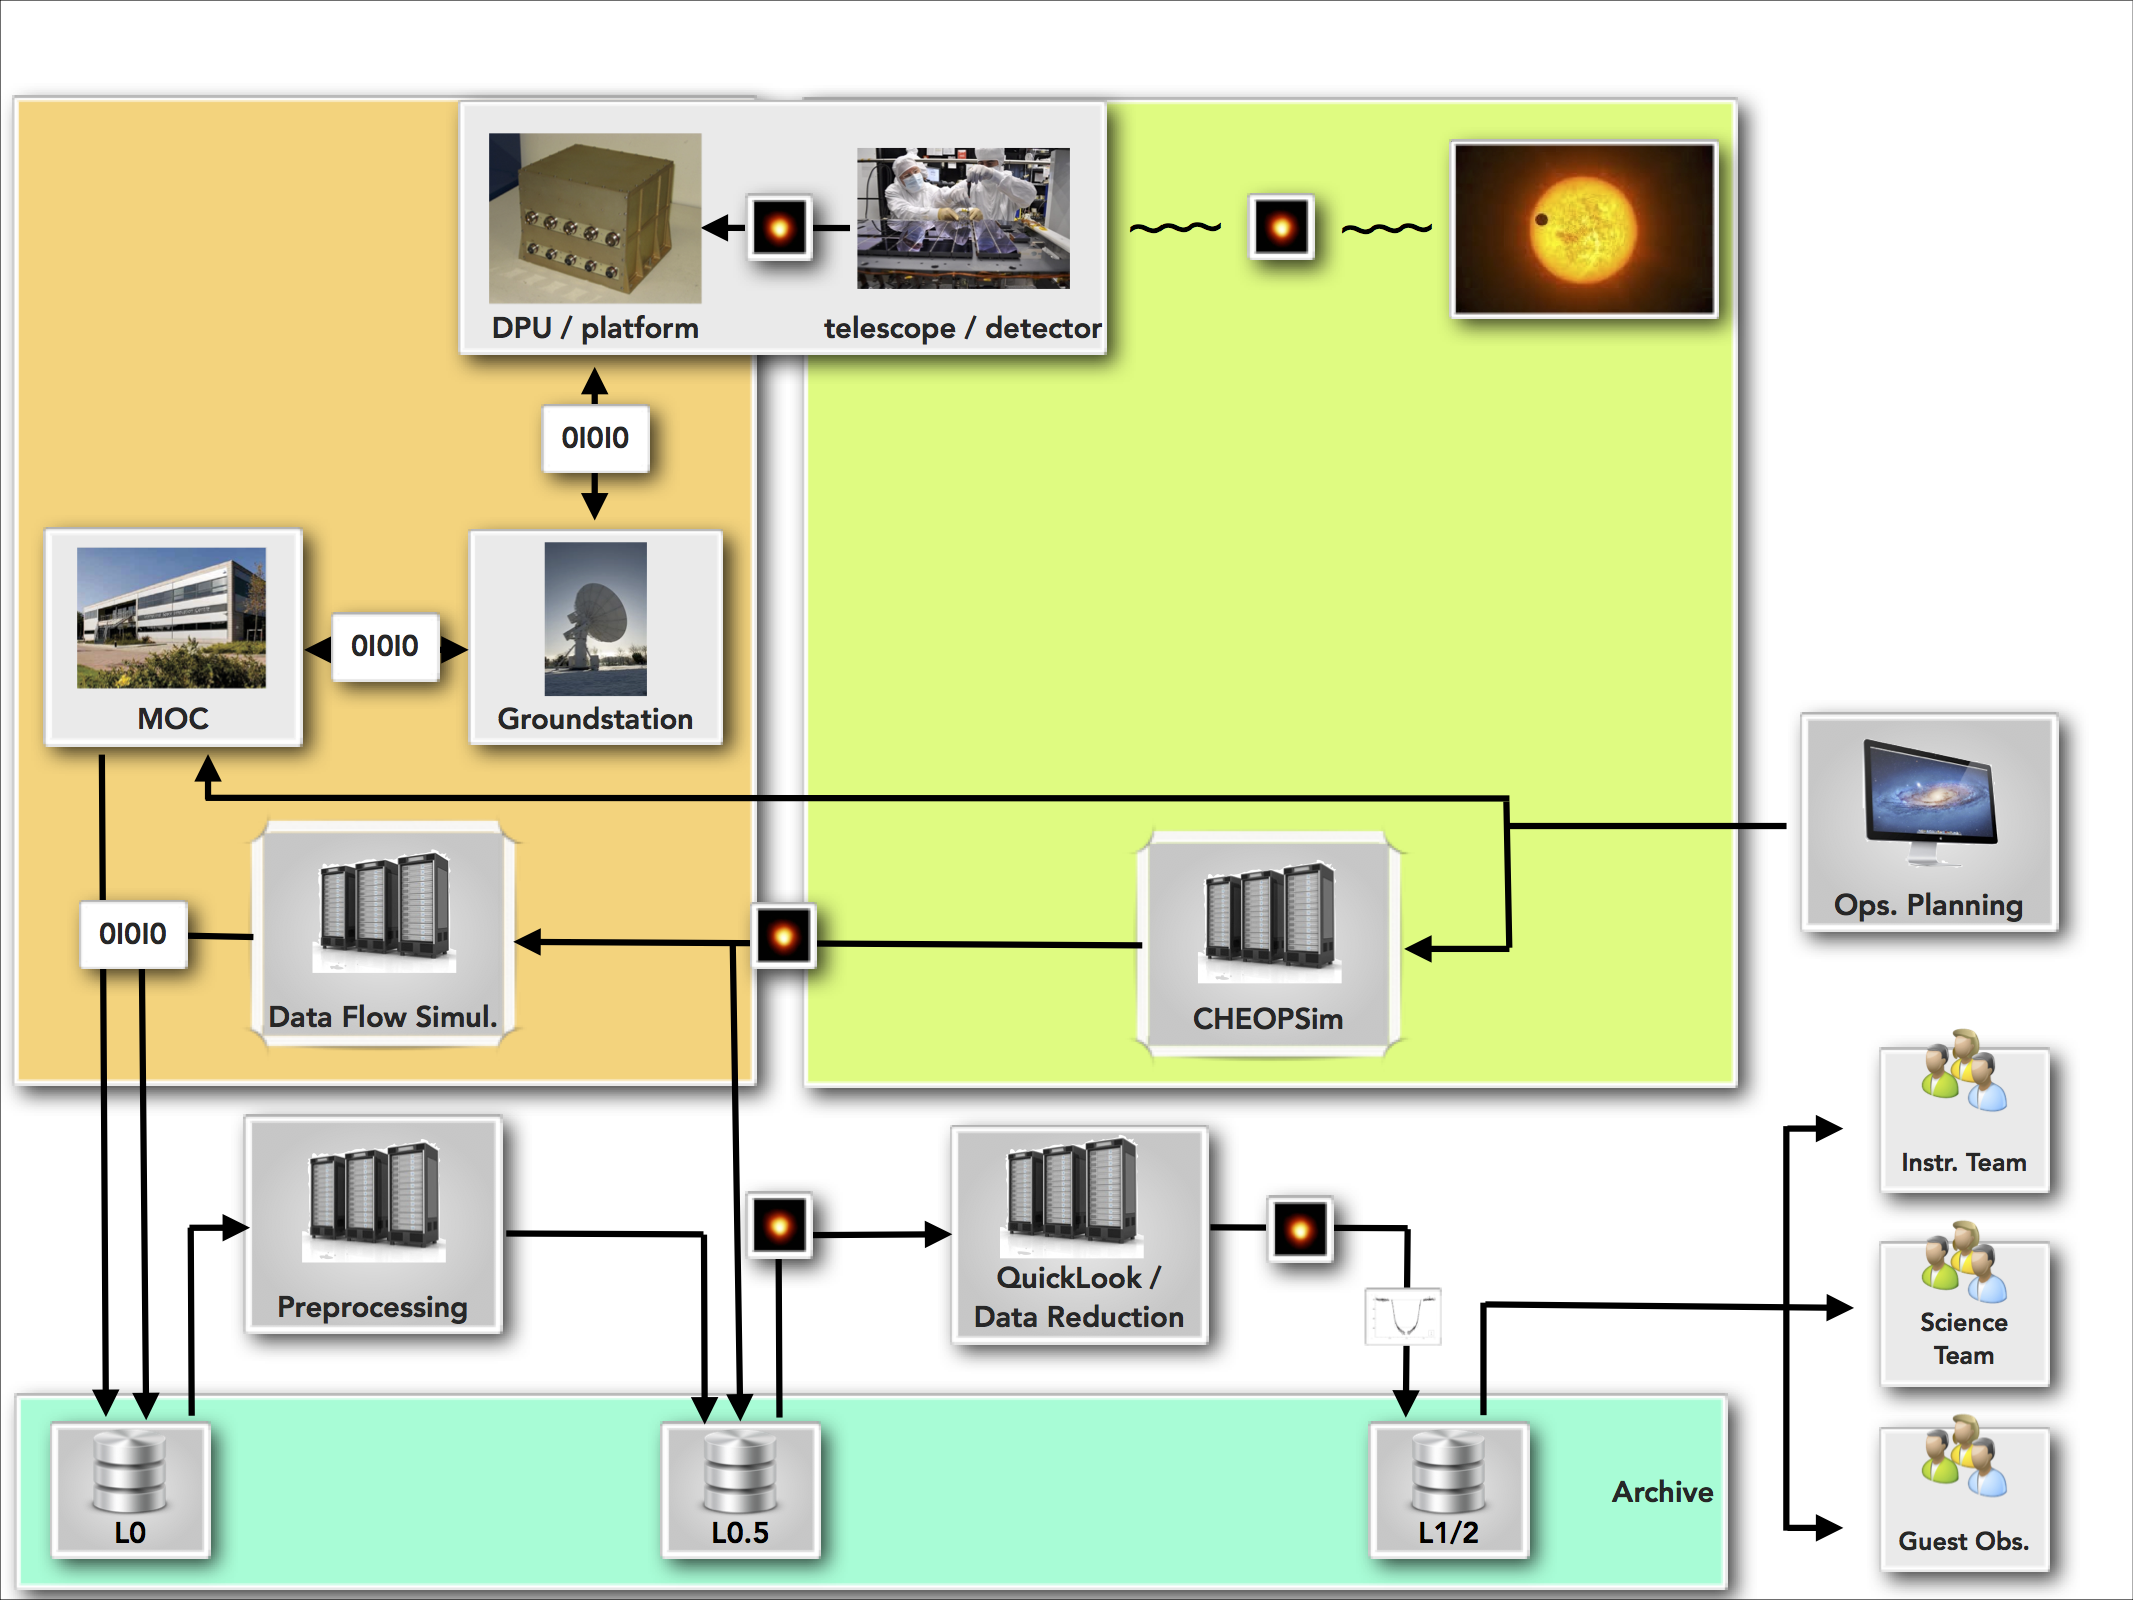
\includegraphics[width=0.5cm]{cheops_data_flow.png}}
    \ifpdf
    {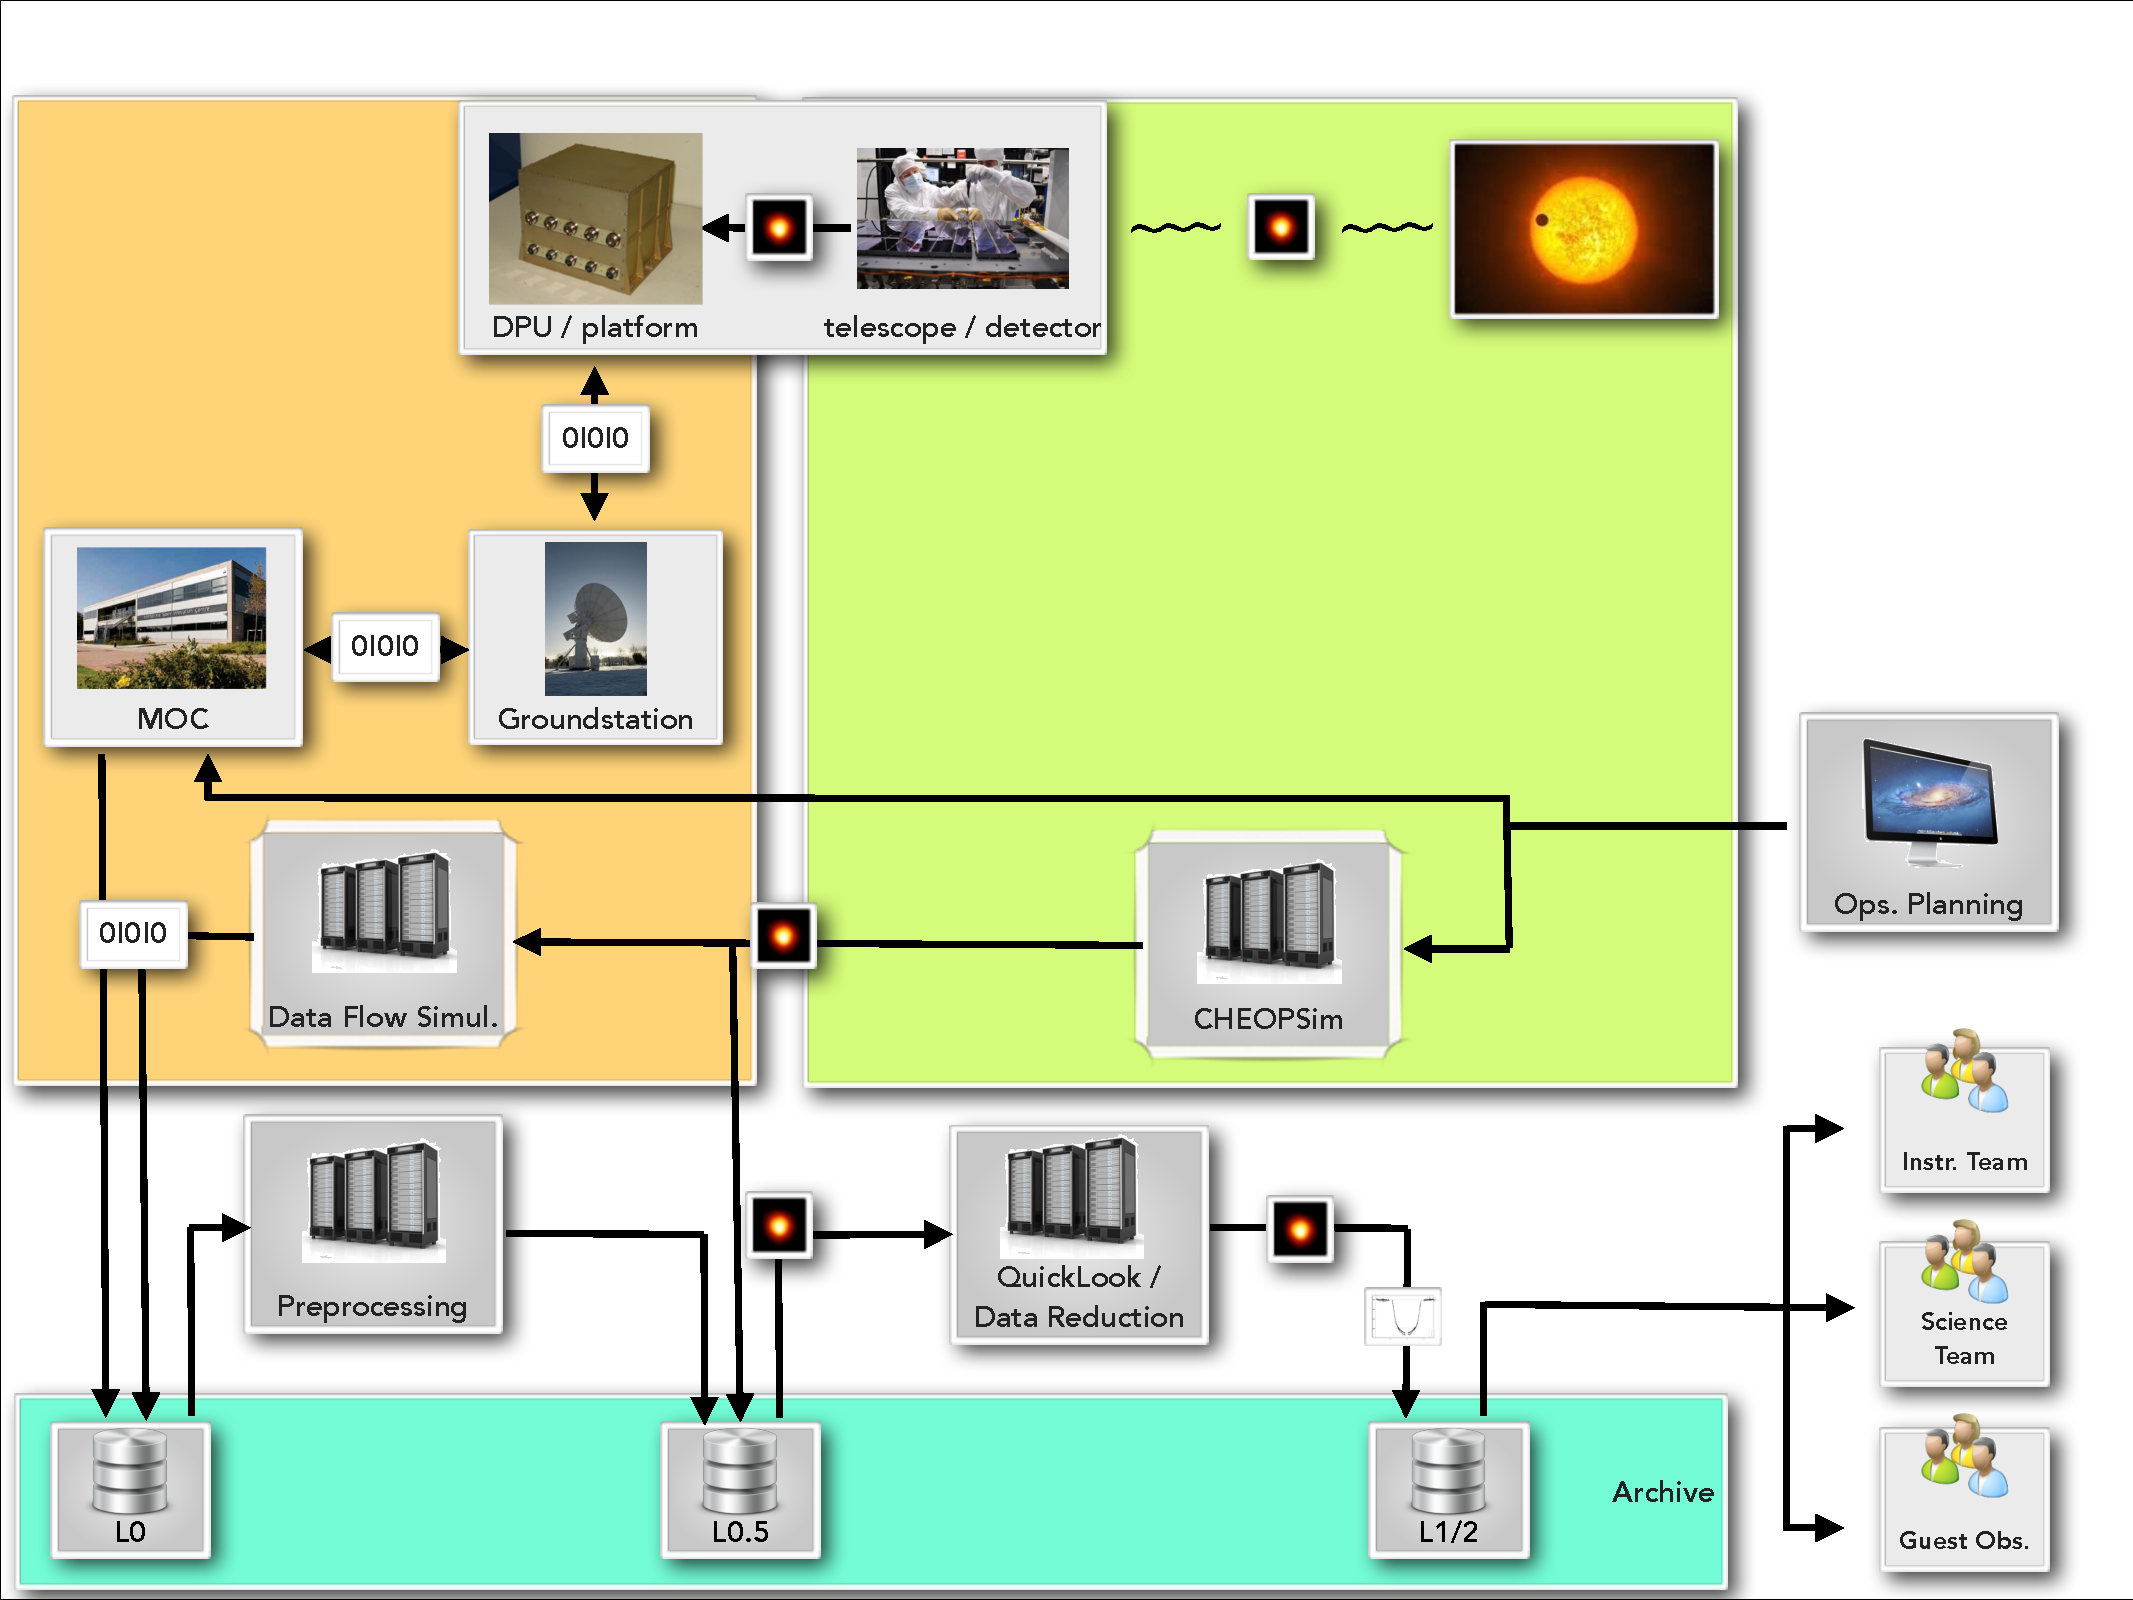
\includegraphics[width=0.8\textwidth]{cheops_data_flow.pdf}}
    \else
    {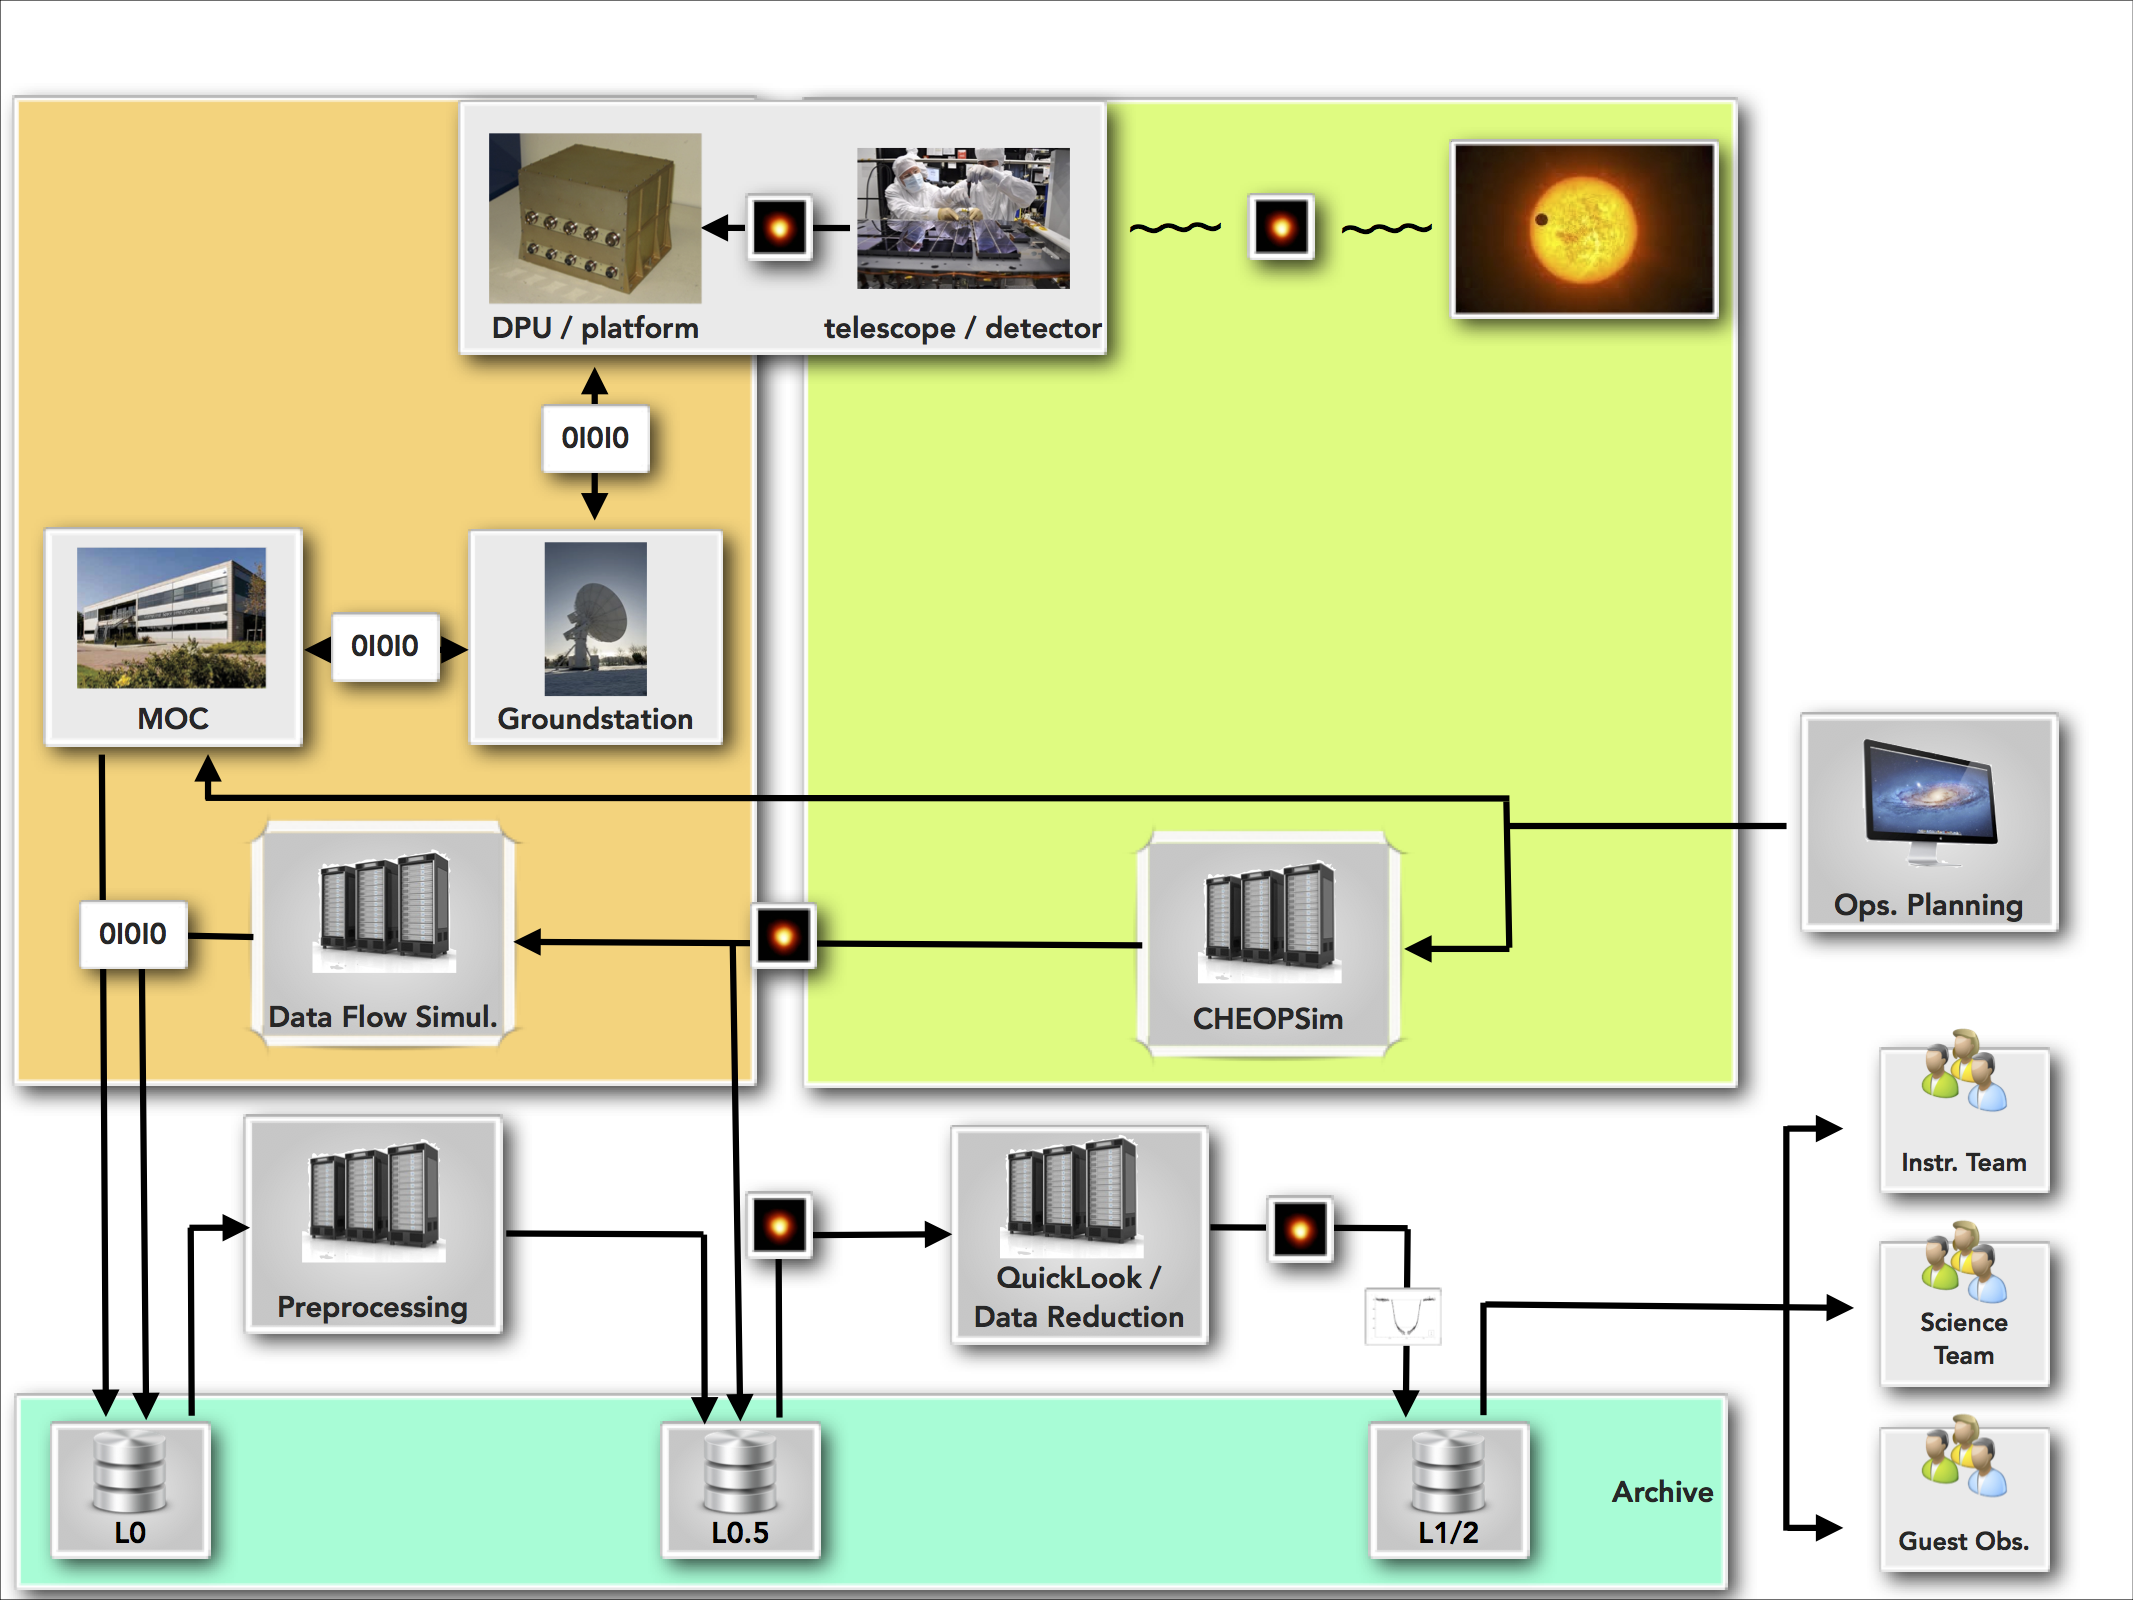
\includegraphics[width=0.8\textwidth]{cheops_data_flow.png}}
    \fi
    \caption{CHEOPS data flow diagram. The output of CHEOPSim can be used as input to either the Data Reduction (L0.5) or to the Data Flow Simulator (S0.5).}
    \label{fig:dataflow}
  \end{center}
\end{figure}

\subsection{Components}
CHEOPSim consists of four main components, referred to as “simulators”, corresponding to the four main aspects of the simulation:
\begin{enumerate}
\item Source Simulator (Section~\ref{sec:Source}):  Modelling of the positions and time variation of fluxes of stars in the field of view.
\item Satellite Simulator (Section~\ref{sec:Satellite}):  Modelling of quantities which vary as a function of the spacecraft orbit, including jitter, FOV rotation, temperature, stray light and particle flux.
\item Telescope Simulator (Section~\ref{sec:Telescope}):  Modelling of the telescope optics, including projection of the FOV onto the focal plane, modelling of the PSF and optical transmission.
\item Detector Simulator (Section ~\ref{sec:Detector}):  Modelling of the CCD response, including photon noise, flat field, dark current, electronic bias and gain, frame transfer, cosmic rays, and bad pixels. 
\end{enumerate}

\subsection{Software Overview}
CHEOPSim is written in C++ and has modular structure, with one module (implemented as a C++ class) corresponding to each functional element of the simulation. This allows different parts of the functionality to be switched on or off independently, within restrictions determined by inter-module dependencies. A description of the functionality implemented in each module is described in sections~\ref{sec:Source} to \ref{sec:Detector}.
The list of modules to be run, together with the configuration parameters for each module are defined via a configuration file in xml format, which can be generated via a \href{https://pichpsweb00.isdc.unige.ch:8443/cheopsim/}{web
  form}, as described in Section~\ref{sec:config}.

\clearpage
\section{Configuration}
\label{sec:config}
The CHEOPSim configuration is defined via an xml file, structured according to the
\href{https://htmlpreview.github.io/?https://github.com/davefutyan/common_sw/blob/master/doc/manual_cxx/group___prog_param.html}{Program
  Params} interface of the CHEOPS
\href{https://htmlpreview.github.io/?https://github.com/davefutyan/common_sw/blob/master/doc/manual_cxx/index.html}{Common
  Software} package.
A \href{https://github.com/davefutyan/CHEOPSim/blob/master/simulator/conf/runCHEOPSim.xml}{default version of the configuration file} is provided.
The configuration xml file can be edited directly, or it can be generated using the \href{https://pichpsweb00.isdc.unige.ch:8443/cheopsim/}{web interface}.

The configuration requires the user to provide values for a number of parameters. Both the web interface and the default xml file provide default values for all parameters, which can be modified by the user. The Visit configuration, defining top level parameters such as the start time and duration of the simulation, is described in Section~\ref{sec:time}. The description of the parameters for each of the various modules can be found in corresponding subsections of Sections~\ref{sec:Source} to \ref{sec:Detector}.

\htmlanchor{time}
\subsection{Visit Configuration}
\label{sec:time}

The parameters used to define the Visit are listed in Tables~\ref{tab:time1} to \ref{tab:time3} . These parameters define the start time and duration of the simulation, the exposure time (which defines the time resolution of the simulation), the number of output images which will be produced (stacked and unstacked), and the pointing direction. The web interface allows the user to define each of these parameters manually, or to instead upload an \href{https://htmlpreview.github.io/?https://github.com/davefutyan/common_sw/blob/master/doc/fits_data_model/MPS_PRE_Visits.html}{MPS\_PRE\_Visits} file from which the values of the parameters are read. If the MPS\_PRE\_Visits option is used, the MPS\_PRE\_Visits table is also used to define the CCD margin mode (see Section~\ref{sec:ccdMargins}) and readout mode (see Section~\ref{sec:DarkCurrentGenerator}).

The simulation executes as a loop over a sequence of time steps, where the duration of each time step is an integer number of seconds. For exposure durations greater than or equal to 1 second, the time step is equal to the exposure duration (required to be an integer). For exposure durations between 0 and 1 second (a non-integer value is allowed for this case), the time step is 1 second. The minimum value of 1 second for the time step is consistent with the fact that the time to read out an image is around 1 second in bright star mode. For each simulated exposure, temporal oversampling of the PSF position can be performed via an optional parameter in the PSFGenerator module (see Section~\ref{sec:PSFGenerator}).  If this option is specified, the variation of the PSF position due to jitter and roll angle is sampled with a 1 second time resolution and combined over the exposure duration.  This temporal oversampling is contained within the PSFGenerator module and does not affect other modules.

\begin{table}[hb]
  \caption{Input parameters to define the Visit configuration using MPS\_PRE\_Visits}

  \htmlanchor{visitFile}
  \begin{tabular}{| l | p{13cm} |}
    \hline 
    {\bf Parameter} & MPS\_PRE\_Visits filename\\
    {\bf Unit} & \\
    {\bf Type / Format} & string\\
    {\bf Default value} & null\\
    {\bf Comments} & If specified, the Observation ID is used to determine which row to read from the file, and parameters from that row are used to override the settings of the other parameters in this table.\\
    \hline
  \end{tabular}
  \bigskip

  \htmlanchor{obsId}
  \begin{tabular}{| l | p{13cm} |}
    \hline
    {\bf Parameter} &  Observation ID\\
    {\bf Unit} & \\
    {\bf Type / Format} & integer\\
    {\bf Default value} & CHEOPSim job ID\\
    {\bf Comments} & The value is used to determine which row is read from the MPS\_PRE\_Visits file if provided. If no value is provided, the value is set to the CHEOPSim job ID. The value appears in header keywords of the output FITS files.\\
    \hline
  \end{tabular}
  \bigskip

  \label{tab:time1}
\end{table}

\begin{table}[hb]
  \caption{Input parameters to define the Visit configuration manually (part 1)}

  \htmlanchor{startTime}
  \begin{tabular}{| l | p{13cm} |}
    \hline 
    {\bf Parameter} &  Start date and time of the simulation\\
    {\bf Unit} & day:month:year hours:minutes:seconds\\
    {\bf Type / Format} & string, format: YYYY-MM-DD HH:MM:SS[.SSS]\\
    {\bf Default value} & 2019-09-01 12:00:00\\
    {\bf Comments} & The part of the format in square brackets is optional\\
    \hline
  \end{tabular}
  \bigskip

  \htmlanchor{exposureTime}
  \begin{tabular}{| l | p{13cm} |}
    \hline
    {\bf Parameter} &  Exposure duration\\
    {\bf Unit} & seconds\\
    {\bf Type / Format} & double\\
    {\bf Default value} & 10\\
    {\bf Comments} & Value will be rounded to the nearest integer except for values between 0 and 1.\\
    \hline
  \end{tabular}
  \bigskip

  \htmlanchor{repetitionPeriod}
  \begin{tabular}{| l | p{13cm} |}
    \hline
    {\bf Parameter} &  Repetition period (interval between the start of consecutive exposures)\\
    {\bf Unit} & seconds\\
    {\bf Type / Format} & double\\
    {\bf Default value} & 0\\
    {\bf Comments} & If the value is 0 (default), CHEOPSim automatically sets the repetition period: For exposure durations shorter than 1s, the repetition period is set to the exposure duration plus 1 second. For  exposure durations longer than 1 second, the  repetition period is set to the nearest integer greater than the exposure duration (the integer rounding is so that the cadence matches that of the jitter sampling).\\
    \hline
  \end{tabular}
  \bigskip

  \htmlanchor{exposuresPerStack}
  \begin{tabular}{| l | p{13cm} |}
    \hline
    {\bf Parameter} & Number of exposures per stacked image\\
    {\bf Unit} & \\
    {\bf Type / Format} & integer\\
    {\bf Default value} & 6\\
    {\bf Comments} & There are 28 allowed values, according to a \href{https://github.com/davefutyan/CHEOPSim/blob/master/resources/LUT_image_stacking.txt}{Look Up Table}. In the web interface, the value is set automatically depending on the exposure time, according to the LUT. The value is automatically updated if the exposure time is changed. The automatic value can be overridden by the user. The automatic value as a function of the exposure time is illustrated in Figure~\ref{fig:LUT_image_stacking}.\\
    \hline
  \end{tabular}
  \bigskip

  \htmlanchor{numberOfStackedImages}
  \begin{tabular}{| l | p{13cm} |}
    \hline
    {\bf Parameter} &  Number of stacked images\\
    {\bf Unit} & \\
    {\bf Type / Format} & integer\\
    {\bf Default value} & 6\\
    {\bf Comments} & Total number of stacked images to be produced in the simulation. \\
    \hline
  \end{tabular}
  \bigskip

  \label{tab:time2}
\end{table}

\begin{table}[hb]
  \caption{Input parameters to define the Visit configuration manually (part 2)}

  \htmlanchor{pointingRA}
  \begin{tabular}{| l | p{13cm} |}
    \hline 
    {\bf Parameter} & Pointing direction Right Ascension \\
    {\bf Unit} & hours:mins:secs or degrees\\
    {\bf Type / Format} & HH:MM:SS[.SSS] or double\\
    {\bf Default value} & 00:00:00.0\\
    {\bf Comments} & RA corresponding to the centre of the FOV. The value will be overridden by the coordinates of the target star if the parameter requesting this in the {\it StarProducer} module is set to true (see Table~\ref{tab:fovInputs}).\\
    \hline
  \end{tabular}
  \bigskip

  \htmlanchor{pointingDec}
  \begin{tabular}{| l | p{13cm} |}
    \hline 
    {\bf Parameter} & Pointing direction declination\\
    {\bf Unit} & degrees:armins:arcsecs or degrees\\
    {\bf Type / Format} & DD:MM:SS[.SSS] or double\\
    {\bf Default value} & 00:00:00.0\\
    {\bf Comments} & Declination corresponding to the centre of the FOV. The value will be overridden by the coordinates of the target star if the parameter requesting this in the {\it StarProducer} module is set to true (see Table~\ref{tab:fovInputs}).\\
    \hline
  \end{tabular}
  \bigskip

  \htmlanchor{doFullFrame}
  \begin{tabular}{| l | p{13cm} |}
    \hline 
    {\bf Parameter} & doFullFrame: Set to true to generate a full frame image corresponding to the first exposure of the simulation.\\
    {\bf Unit} & \\
    {\bf Type / Format} & boolean\\
    {\bf Default value} & true\\
    {\bf Comments} &  Will be written to an output fits file if ImageWriter is switched on.\\
    \hline
  \end{tabular}

  \label{tab:time3}
\end{table}

The number of unstacked images, and the duration of the simulation are determined from the parameters in Table~\ref{tab:time2} as follows:

\begin{center}
No. of unstacked images = no. of stacked images * no. of exposures per stacked image\\
Duration of simulation = no. of unstacked images * exposure duration\\
\end{center}

If the Visit is defined by uploading an MPS\_PRE\_Visits file, the no. of unstacked images and exposure duration are determined by the values of N\_WINDOWFRAME\_EXP and EXP\_TIME, respectively, in the row of the MPS\_PRE\_Visits table determined by the Observation ID.

The total duration of the simulation in hours is displayed in the \href{https://pichpsweb00.isdc.unige.ch:8443/cheopsim/}{web
interface}, being calculated automatically from the above inputs.

% Configuration parameters other than those specified in Table~\ref{tab:time2} are specific to a particular module, and are defined in the subsection corresponding to each module in Sections~\ref{sec:Source} to \ref{sec:Detector}.

\clearpage
\section{Source Simulator}
\label{sec:Source}

The Source Simulator models the positions and time variation of fluxes for all stars in the field of view. Each of Sections~\ref{sec:StarProducer} to \ref{sec:StrayLightGenerator} corresponds to a CHEOPSim software module with the indicated name.

\htmlanchor{StarProducer}
\subsection{Field of View and Stellar Flux:  {\it StarProducer}}
\label{sec:StarProducer}
  \htmlanchor{FOV}
\subsubsection{Field of View}
\label{sec:fov}
The field of view (FOV) is defined to be a circle enclosing the region of sky to which the CCD imaging region being considered is exposed for all possible rotation angles. The inputs required to define the field of view are shown in Table~\ref{tab:fovInputs}.
Stars are processed if they lie within the FOV which can take one of three possible values, as illustrated in Figure~\ref{fig:fov}:
\begin {enumerate}
\item The imaging sub-array is a square of size 200$\times$200 pixels, which for a plate scale of 1.002 arcsecond per pixel corresponds to an FOV radius of 141 arcseconds.  In order to include partial PSFs whose centres lie outside the frame, a margin of 25 pixels is added, such that the FOV is defined as a circle enclosing 250$\times$250 pixels, corresponding to an FOV radius of 177 arcseconds.
\item If frame transfer is simulated, stars located within a strip of width 200 pixels extending from the top to the bottom of the exposed part of the CCD will also affect the exposure, such that the total imaging region becomes a rectangle of dimension 200$\times$1024 pixels, and the corresponding FOV radius, including a 25 pixel margin is 551 arcseconds.
\item For generation of 1024$\times$1024 pixel full frame images the FOV radius is set to 759 arcseconds.
\end{enumerate}

\begin{figure}[hbtp]
  \begin{center}
    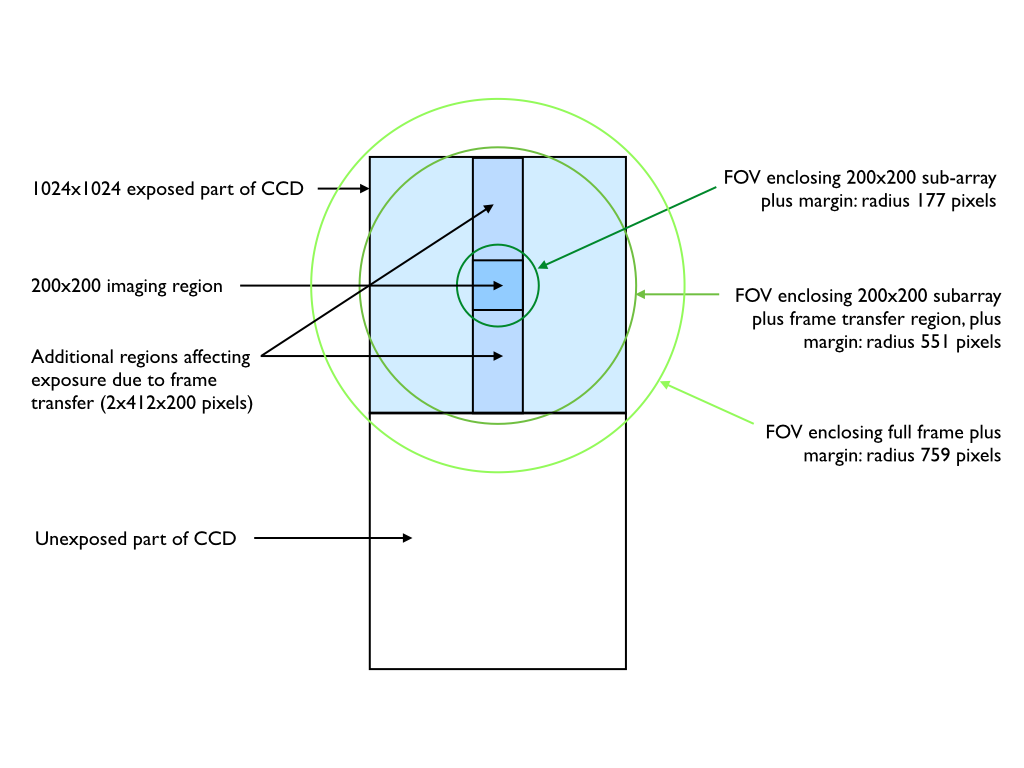
\includegraphics[width=\textwidth]{fov.png}
    \caption{Definition of Field of View with respect to the CCD dimensions.}
    \label{fig:fov}
  \end{center}
\end{figure}

\begin{table}[hb]
  \caption{Input parameters to define the field of view}

  \htmlanchor{FOVradius}
  \begin{tabular}{| l | p{13cm} |}
    \hline 
    {\bf Parameter} & Field of View radius\\
    {\bf Unit} & arcseconds\\
    {\bf Type / Format} & double\\
    {\bf Default value} & 551 (see text for explanation)\\
    {\bf Comments} & Radius of the FOV.  Any stars located more than this distance from the pointing direction are excluded from the simulation.\\
    \hline
  \end{tabular}
  \bigskip

  \htmlanchor{minMagnitude}
  \begin{tabular}{| l | p{13cm} |}
    \hline 
    {\bf Parameter} & Faintest magnitude for stars in the FOV\\
    {\bf Unit} & \\
    {\bf Type / Format} & double\\
    {\bf Default value} & 19\\
    {\bf Comments} & Permitted values are in the range 10 to 20. Any stars in the FOV with magnitude fainter than this value will be excluded from the simulation\\
    \hline
  \end{tabular}
  \bigskip

  \begin{tabular}{| l | p{13cm} |}
    \hline 
    {\bf Parameter} & Use the target star coordiantes to define the pointing direction\\
    {\bf Unit} & \\
    {\bf Type / Format} & boolean\\
    {\bf Default value} & true\\
    {\bf Comments} & If set to true, the coordinates of the target star override the pointing direction defined in the Visit Configuration (Section~\ref{sec:time}), whether defined manually or via an uploaded MPS\_PRE\_Visits file. This guarantees that the target star is exactly centred along the boresight in the absence of jitter. Note that in general the RA and dec of the target star in EXT\_PRE\_StarCatalogue will differ slightly from the pointing direction defined in MPS\_PRE\_Visits due to corrections for precession of the Earth's axis and for proper motion of the target applied in the former.\\
    \hline
  \end{tabular}
  \bigskip

  \label{tab:fovInputs}
\end{table}

% \begin{table}
%   \begin{tabular}{| p{3cm} | c | c | c | p{3cm} |}
%     \hline
% {\bf Quantity} & \bf{Unit} & \bf{Type/} & \bf{Default} & \bf{Description}\\
% & &  \bf{Format} & \bf{value} & \\
% \hline
% Field of View radius & arcseconds & double & 521.67 & Radius of the FOV (see text for details)\\
% \hline
% Pointing direction Right Ascension & hours:mins:secs & HH:MM:SS[.SSS] & 00:00:00.0 & RA corresponding to the centre of the FOV\\
% \hline
% Pointing direction declination & degrees:armins:arcsecs & DD:MM:SS[.SSS] & 00:00:00.0 & Declination corresponding to the centre of the FOV\\
% \hline
% Faintest magnitude for stars in the FOV &  & integer & 20 & Any stars
% in the FOV with magnitude below this value will be excluded from the
% simulation\\
% \hline
% \end{tabular}
% \caption{Inputs to define the field of view}
% \label{tab:fovInputs}
% \end{table}

\clearpage

\htmlanchor{stars}
\subsubsection{Star Field}
\label{sec:stars}

An unlimited number of stars can be added to the field of view. Note that the CPU time required for the simulation increases in proportion to the number of stars. The parameters required for each star are indicated in Table~\ref{tab:star}. The web interface permits the user to provide the list of stars in one of three ways:
\begin{enumerate}
\item The parameters for the target star can be directly entered using fields provided in the web interface. The same information for up to 9 additional stars can optionally be provided using the ``Add star'' button.
\item The parameters for an unlimited number of stars can be provided by uploading an FITS file with data structure \href{https://htmlpreview.github.io/?https://github.com/davefutyan/common_sw/blob/master/doc/fits_data_model/EXT_PRE_StarCatalogue.html}{EXT\_PRE\_StarCatalogue} or \href{https://htmlpreview.github.io/?https://github.com/davefutyan/common_sw/blob/master/doc/fits_data_model/EXT_DRFT_StarCatalogue.html}{EXT\_DRFT\_StarCatalogue}.
\item The parameters for an unlimited number of stars can be provided by uploading an ASCII file, containing a line for each star, with the target star on the first line. The required format for each line is whitespace or tab separated values for the parameters defined in Table~\ref{tab:star}. The two following example text files are equivalent:\\

\begin{tabular}{l l l l}
00:00:00.0 & 00:00:00.0 & 9. & G0 \\
00:00:03.33 & 00:00:50.0 & 12. & K0 \\
-00:00:03.33 & 00:00:50.0 & 12. & K0 \\
00:00:03.33 & -00:00:50.0 & 12. & K0 \\
-00:00:03.33 & -00:00:50.0 & 12. & K0 \\
\end{tabular}

\begin{tabular}{l l l l}
0.0 & 0.0 & 9. & G0 \\
0.0139 & 0.0139 & 12. & K0 \\
-0.0139 & 0.0139 & 12. & K0 \\
0.0139 & -0.0139 & 12. & K0 \\
-0.0139 & -0.0139 & 12. & K0 \\
\end{tabular}

\end{enumerate}

If a star has a position which lies outside the field of view, or has a magnitude fainter than the faintest magnitude parameter in Table~\ref{tab:fovInputs}, the star is omitted from the simulation.

\begin{table}[hb]
  \caption{Input parameters for each star}

  \begin{tabular}{| l | p{13cm} |}
    \hline 
    {\bf Parameter} & Right Ascension \\
    {\bf Unit} & hours:mins:secs or degrees\\
    {\bf Type / Format} & HH:MM:SS[.SSS] or double\\
    {\bf Default value} & 00:00:00.0\\
    {\bf Comments} & \\
    \hline
  \end{tabular}
  \bigskip

  \begin{tabular}{| l | p{13cm} |}
    \hline 
    {\bf Parameter} & Declination\\
    {\bf Unit} & degrees:armins:arcsecs or degrees\\
    {\bf Type / Format} & DD:MM:SS[.SSS] or double\\
    {\bf Default value} & 00:00:00.0\\
    {\bf Comments} & \\
    \hline
  \end{tabular}
  \bigskip

  \begin{tabular}{| l | p{13cm} |}
    \hline 
    {\bf Parameter} & Magnitude\\
    {\bf Unit} & \\
    {\bf Type / Format} & double\\
    {\bf Default value} & 0.0\\
    {\bf Comments} & If value is fainter than the faintest magnitude defined in Table~\ref{tab:fovInputs}, the star is excluded from the simulation\\
    \hline
  \end{tabular}
  \bigskip

  \begin{tabular}{| l | p{13cm} |}
    \hline 
    {\bf Parameter} & Spectral Type\\
    {\bf Unit} &\\
    {\bf Type / Format} & Enum. For permitted values, see Tables~\ref{tab:starProperties1} and \ref{tab:starProperties2}.\\
    {\bf Default value} & G0\\
    {\bf Comments} & \\
    \hline
  \end{tabular}
  \bigskip

  \label{tab:star}
\end{table}

\clearpage

\htmlanchor{doBackgroundStars}
\subsubsection{Background Star Field}
\label{sec:starField}

In addition ot the stars explicitly defined in Section~\ref{sec:stars}, a background star field can be generated according to one of three predefined lists, constructed from real star fields. The lists are provided by Bastien Courcol, established using the USNO-B catalog. Each of the lists corresponds to the set of stars within an FOV radius of 730 arcseconds, centred 10 arcminutes away from a potential CHEOPS target. The potential targets together with the number of background stars in each list are indicated in Table~\ref{tab:starFields}.

\begin{table}[hb]
  \begin{center}
  \caption{Background Star Fields}
  \begin{tabular}{| c | c | c | c | c | c | c |}
    \hline
Target star & Vmag & Galactic & Galactic & Number & Contamination & Star list\\
 & & longitude & latitude & of stars & & \\
    \hline
HAT-P-26 & 11.76 & 346.5135 & +59.8731 & 979 & {\bf Low} & \href{https://github.com/davefutyan/CHEOPSim/blob/master/resources/Low_field.txt}{Low\_field.txt} \\
BD-082823 & 9.86 & 248.4966 & +34.7560 & 1673 & {\bf Medium} & \href{https://github.com/davefutyan/CHEOPSim/blob/master/resources/Medium_field.txt}{Medium\_field.txt} \\
HD154088 & 6.58 & 355.2373 & +07.6735 & 29169 & {\bf Extreme} & \href{https://github.com/davefutyan/CHEOPSim/blob/master/resources/Extreme_field.txt}{Extreme\_field.txt} \\
    \hline
  \end{tabular}
  \label{tab:starFields}
\end{center}
\end{table}

The user can select between these three lists via the web interface, which provides the options ``Low'', ``Medium'' and ``Extreme'' for the background density, corresponding to the three rows of  Table~\ref{tab:starFields} as indicated in the contamination column.

The set of background stars from the specified list, which lie within the field of view radius (see Section~\ref{sec:fov}) and have magnitude brighter than the faintest magnitude parameter defined in Table~\ref{tab:fovInputs}, are added to the field of view defined in Section~\ref{sec:fov}. For a given star list, the user can reduce the number of stars to be processed, thereby reducing the run time of the simulation, by decreasing the value of the magnitude threshold.

The background star fields, as generated in CHEOPSim images, are shown in Figure~\ref{fig:backgroundStars}.

\begin{table}[hb]
  \caption{Input parameters for background star field generation}

  \begin{tabular}{| l | p{13cm} |}
    \hline 
    {\bf Parameter} & Generate background star field\\
    {\bf Unit} & \\
    {\bf Type / Format} & boolean\\
    {\bf Default value} & false\\
    {\bf Comments} & \\
    \hline
  \end{tabular}
  \bigskip

  \htmlanchor{fieldCrowding}
  \begin{tabular}{| l | p{13cm} |}
    \hline 
    {\bf Parameter} & Star field density\\
    {\bf Unit} &\\
    {\bf Type / Format} & string\\
    {\bf Default value} & medium\\
    {\bf Comments} & Permitted values are ``low'', ``medium'' or ``extreme''\\
    \hline
  \end{tabular}
  \bigskip

  \label{tab:backgroundStars}
\end{table}

\begin{figure}[hbtp]
  \begin{center}
    \href{low_field.png}{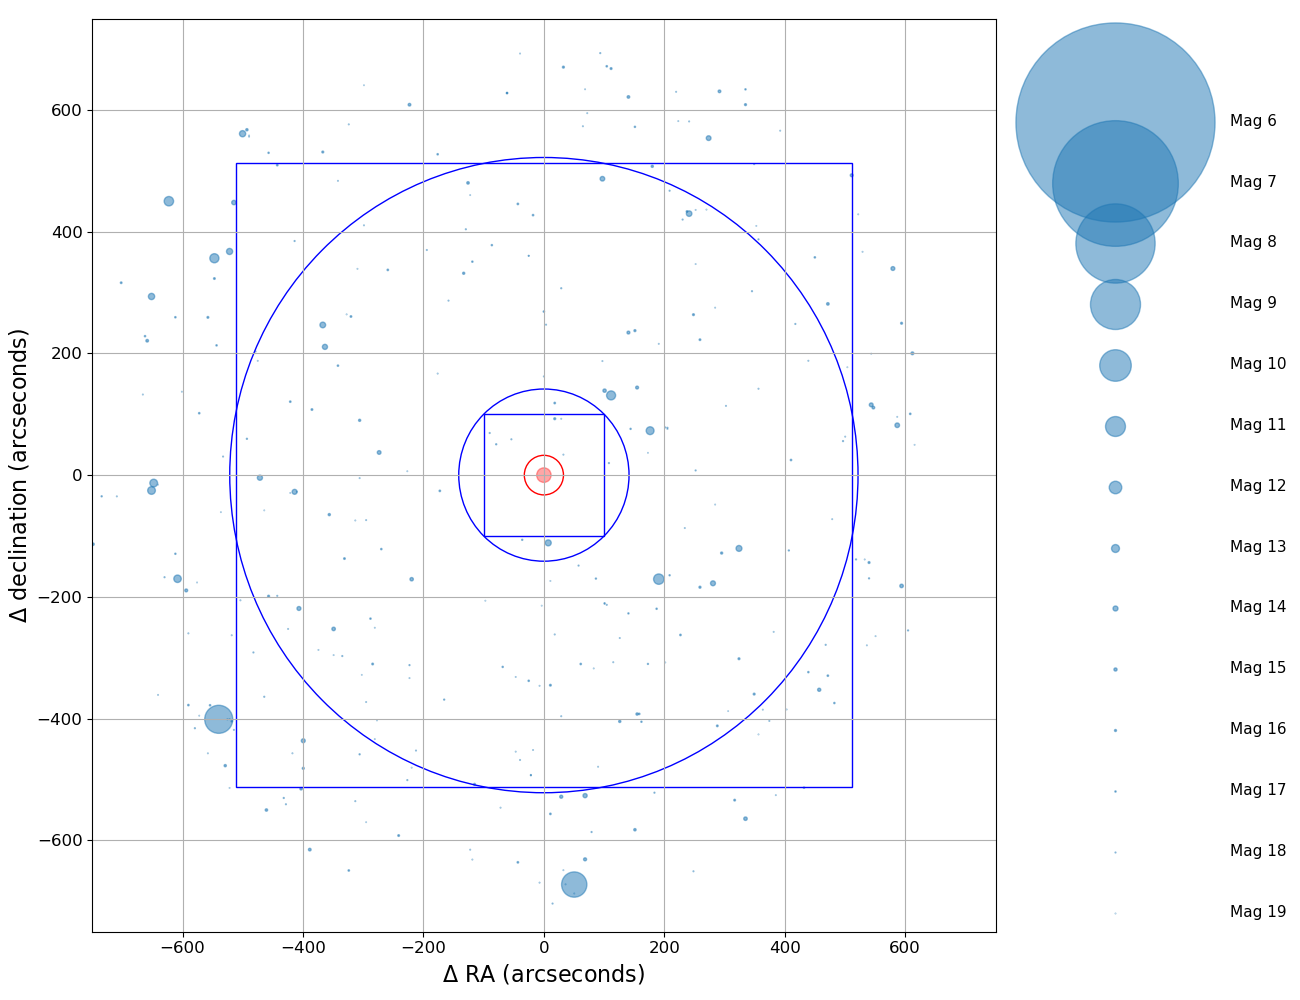
\includegraphics[width=0.49\textwidth]{low_field.png}}
    \href{medium_field.png}{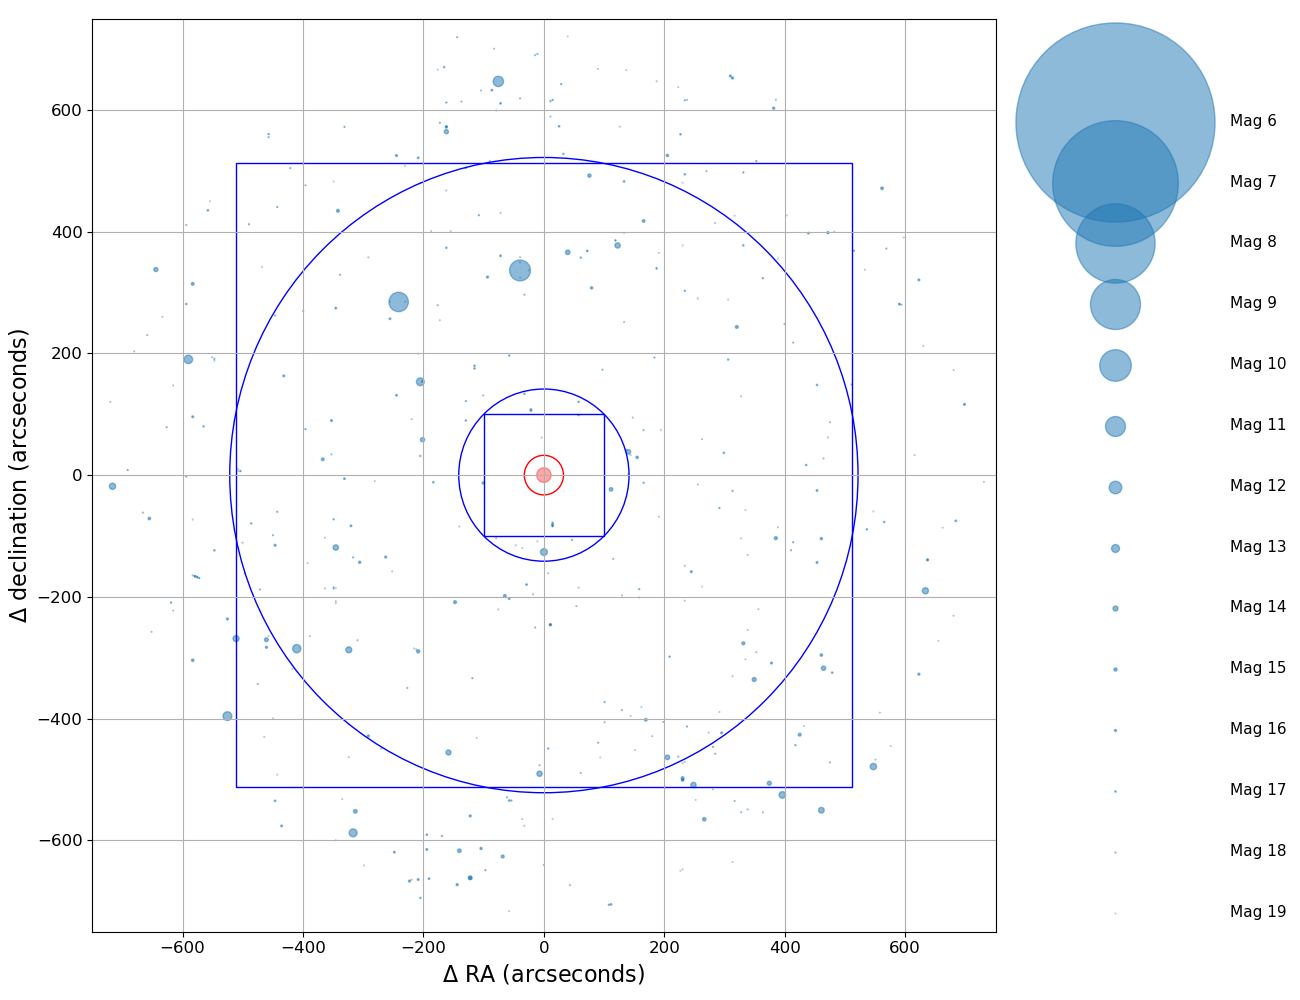
\includegraphics[width=0.49\textwidth]{medium_field.png}}
    \href{extreme_field.png}{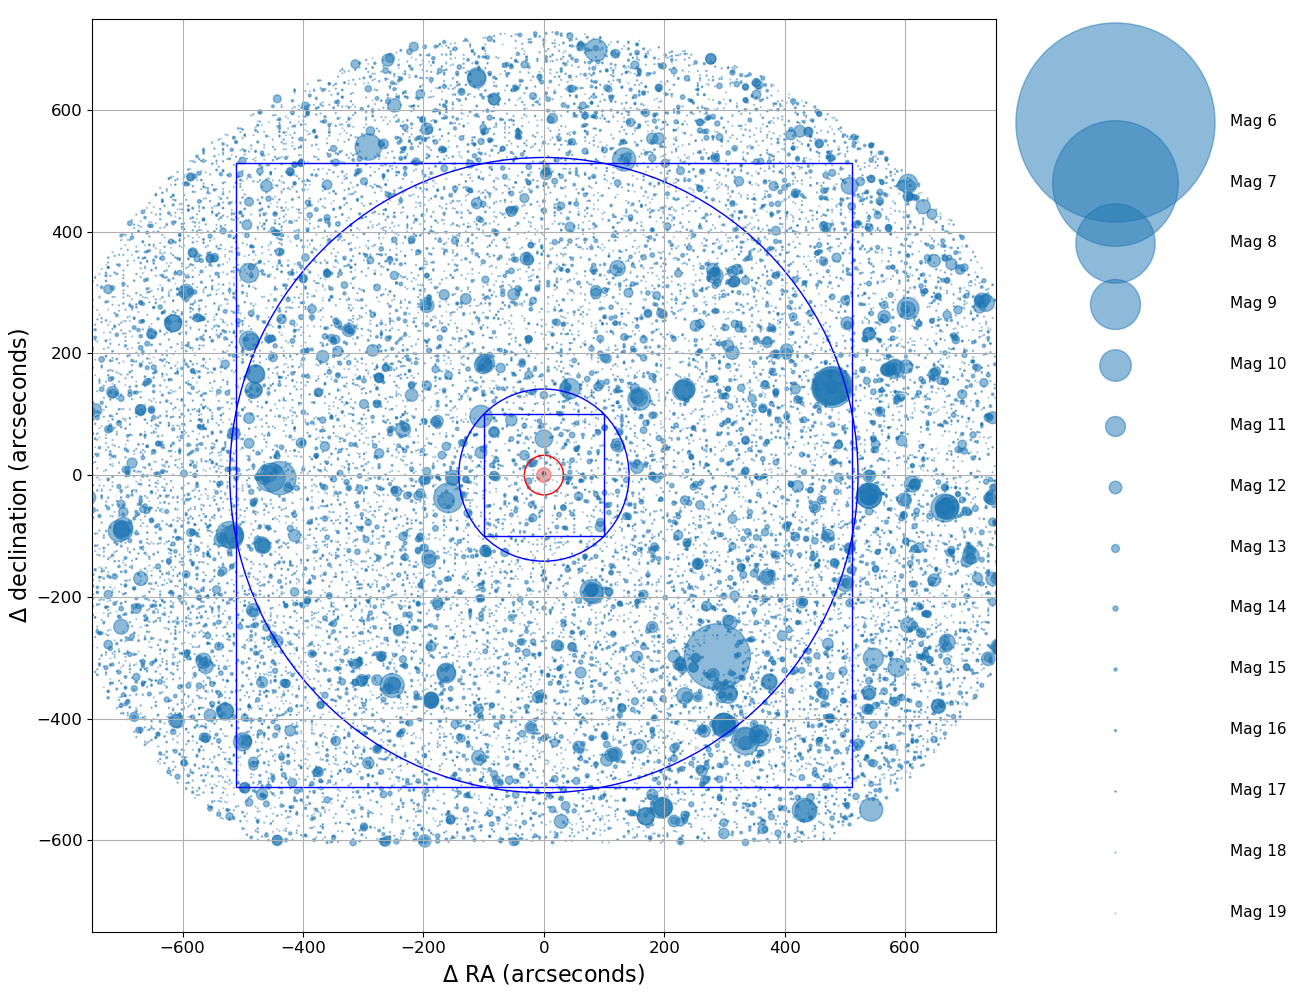
\includegraphics[width=0.49\textwidth]{extreme_field.png}}
    \caption{Background star fields - click for larger versions: low (left), medium (centre) and extreme (right), as defined in Table~\ref{tab:starFields}. Stars located within the inner circle can enter the sub-array (inner square) at some point during field of view rotation. Stars located within the outer circle can generate frame transfer smear trails (see Section~\ref{sec:FrameTransferSmearer}) which can cross the sub-array at some point during field of view rotation. The area of each marker is proportional to the stellar flux. The magnitudes indicated in the scale on the right are CHEOPS magnitudes. The open red circle represents the default aperture used in the photometric extration (radius 32.5 pixels). The filled red circle represents the approximate size of the PSF excluding tails (radius 12 pixels).}
    \label{fig:backgroundStars}
  \end{center}
\end{figure}

\clearpage 
\htmlanchor{SEDs}
\subsubsection{Flux Calculation}
\label{sec:flux}

For each star, the flux spectrum is calculated given the the magnitude and spectral type inputs specified in Table~\ref{tab:star}.  An effective temperature $T_{eff}$ is assigned for each spectral type according to Tables~\ref{tab:starProperties1} and \ref{tab:starProperties2}.  The wavelength spectrum is determined according to one of two methods:
\begin{enumerate}
\item A synthetic Spectral Energy Distribution (SED) is assigned according to the effective temperature, from a version of the \href{https://github.com/davefutyan/CHEOPSim/releases/tag/v1.0}{REF\_APP\_SEDTeff} reference file which can be selected by the user. This is the default method for effective temperatures in the range provided by the reference file (2300K to 7200K for version V0102, covering F, G, K and M type stars). The SEDs were generated using the PHOENIX model~\cite{PHOENIX}.
\item A Planck black body spectrum is generated according to equation~\ref{eq:planck} in 10 angstrom bins. This method is used for effective temperatures higher than 7200K (O, A and B type stars), and optionally for lower effective temperatures. It should be noted that a black body is a poor approximation for M-type stars.
\end{enumerate}
\htmlanchor{userSED}
An option is also provided for the user to upload a file defining a SED for the target star, for example if there is an empirically measured spectrum for a real target being simulated. The format of the file must be a FITS table which includes columns with names ``WAVELENGTH'' and ``FLUX''. The units of the WAVELENGTH column can be either nm or angstroms and must cover the range 330 to 1100nm. The number of rows in that wavength range must not exceed 2000. The units of the ``FLUX'' column are arbitrary as only the shape of the spectrum is relevant, with the normalization being defined as described below.

\begin{table}[hb]
  \begin{center}
  \caption{Effective temperature, stellar radius and stellar mass assigned to spectral types O7 to F9. Values are taken from \cite{stellarParameters}. The stellar radius is calculated from the luminosity and the effective temperature using the relation $L=4\pi R^2 \sigma T_{eff}^4$, assuming $\sigma=5.67036\times10^{-8}$~kg s$^{-3}$ K$^{-4}$ and $L_{\odot}=3.828\times10^{26}$~W. Values assumed for the solar standard gravitational parameter, $\mu_{\odot}=G\cdot M_{\odot}$,  and the solar radius, $R_{\odot}$, are 132712440018~km$^3$s$^{-2}$ and 696342~km, respectively.}
  \begin{tabular}{| c | c | c | c |}
    \hline 
    Spectral type & $T_{eff}$ (Kelvin) & mass ($M_{\odot}$) & radius ($R_{\odot}$)\\
    \hline
O7 & 36500 & 28 & 9.61 \\
O8 & 34500 & 22.9 & 8.74 \\
O9 & 32500 & 19.7 & 8.1 \\
B0 & 31500 & 17.5 & 7.51 \\
B1 & 26000 & 11 & 5.72 \\
B2 & 20600 & 7.3 & 3.84 \\
B3 & 17000 & 5.4 & 3.48 \\
B4 & 16700 & 5 & 3.4 \\
B5 & 15700 & 4.6 & 3.39 \\
B6 & 14500 & 4 & 2.95 \\
B7 & 14000 & 3.9 & 2.99 \\
B8 & 12500 & 3.4 & 2.91 \\
B9 & 10700 & 2.8 & 2.28 \\
A0 & 9700 & 2.3 & 2.08 \\
A1 & 9200 & 2.15 & 1.99 \\
A2 & 8840 & 2.05 & 1.97 \\
A3 & 8550 & 2 & 2.01 \\
A4 & 8270 & 1.9 & 1.94 \\
A5 & 8080 & 1.85 & 1.94 \\
A6 & 8000 & 1.83 & 1.93 \\
A7 & 7800 & 1.76 & 1.85 \\
A8 & 7500 & 1.67 & 1.81 \\
A9 & 7440 & 1.67 & 1.84 \\
F0 & 7220 & 1.59 & 1.78 \\
F1 & 7030 & 1.5 & 1.63 \\
F2 & 6810 & 1.44 & 1.61 \\
F3 & 6720 & 1.43 & 1.59 \\
F4 & 6640 & 1.39 & 1.52 \\
F5 & 6510 & 1.33 & 1.46 \\
F6 & 6340 & 1.25 & 1.36 \\
F7 & 6240 & 1.21 & 1.29 \\
F8 & 6170 & 1.18 & 1.25 \\
F9 & 6040 & 1.14 & 1.23 \\
    \hline
  \end{tabular}
  \label{tab:starProperties1}
  \end{center}
\end{table}

\begin{table}[hb]
  \begin{center}
  \caption{Effective temperature, stellar radius and stellar mass assigned to spectral types G0 to M9. Values are taken from \cite{stellarParameters}. The stellar radius is calculated from the luminosity and the effective temperature using the relation $L=4\pi R^2 \sigma T_{eff}^4$, assuming $\sigma=5.67036\times10^{-8}$~kg s$^{-3}$ K$^{-4}$ and $L_{\odot}=3.828\times10^{26}$~W. Values assumed for the solar standard gravitational parameter, $\mu_{\odot}=G\cdot M_{\odot}$,  and the solar radius, $R_{\odot}$, are 132712440018~km$^3$s$^{-2}$ and 696342~km, respectively.}
  \begin{tabular}{| c | c | c | c |}
    \hline 
    Spectral type & $T_{eff}$ (Kelvin) & mass ($M_{\odot}$) & radius ($R_{\odot}$)\\
    \hline
G0 & 5920 & 1.08 & 1.12 \\
G1 & 5880 & 1.07 & 1.12 \\
G2 & 5770 & 1.02 & 1.01 \\
G3 & 5720 & 1.00 & 1.01 \\
G4 & 5680 & 0.99 & 0.985 \\
G5 & 5660 & 0.98 & 0.981 \\
G6 & 5590 & 0.97 & 0.938 \\
G7 & 5530 & 0.96 & 0.948 \\
G8 & 5490 & 0.94 & 0.908 \\
G9 & 5340 & 0.90 & 0.875 \\
K0 & 5280 & 0.87 & 0.817 \\
K1 & 5170 & 0.85 & 0.813 \\
K2 & 5040 & 0.82 & 0.763 \\
K3 & 4840 & 0.78 & 0.729 \\
K4 & 4620 & 0.73 & 0.689 \\
K5 & 4450 & 0.72 & 0.709 \\
K6 & 4200 & 0.70 & 0.654 \\
K7 & 4050 & 0.64 & 0.613 \\
K8 & 3970 & 0.61 & 0.609 \\
K9 & 3880 & 0.58 & 0.543 \\
M0 & 3850 & 0.58 & 0.526 \\
M1 & 3700 & 0.52 & 0.474 \\
M2 & 3550 & 0.48 & 0.433 \\
M3 & 3400 & 0.43 & 0.371 \\
M4 & 3200 & 0.24 & 0.258 \\
M5 & 3050 & 0.15 & 0.197 \\
M6 & 2800 & 0.10 & 0.131 \\
M7 & 2650 & 0.098 & 0.118 \\
M8 & 2500 & 0.082 & 0.114 \\
M9 & 2450 & 0.065 & 0.0953 \\
    \hline
  \end{tabular}
  \label{tab:starProperties2}
  \end{center}
\end{table}

\begin{equation}
flux_{Planck}(\lambda) = \frac{2hc^2}{\lambda^5}\frac{1}{e^{\frac{hc}{\lambda k_B T_{eff}}}-1}
\label{eq:planck}
\end{equation}

The spectra defined above provide the energy flux. The photon flux is obtained by dividing by the energy per photon:
$$photonflux(\lambda)=\frac{energyflux(\lambda)}{hc/\lambda}$$

\htmlanchor{passband}
The photon flux spectrum is first normalized to magnitude 0.035 by normalizing to the integrated flux of Vega in a reference band which can be chosen by the user to be either the Gaia passband or the V-band. The Gaia passband is recommended as it is much more similar to the CHEOPS passband (see Figure~\ref{fig:fluxnorm} (right)), but the option to use the original implementation which used the V-band is retained. The spectrum of the star (SED or black body as described above), and the spectrum of Vega (Figure~\ref{fig:fluxnorm} (left), divided by $hc/\lambda$ in order to convert to photons), are each scaled by the transmission curve of the chosen reference band shown in Figure~\ref{fig:fluxnorm} (right).  The integrals of the two resulting distributions are calculated using a wavelength resolution of 1~nm.  The spectrum of the star is normalized according to the ratio of these integrals (equation~\ref{eq:fluxnorm}).

\begin{figure}[hbtp]
  \begin{center}
    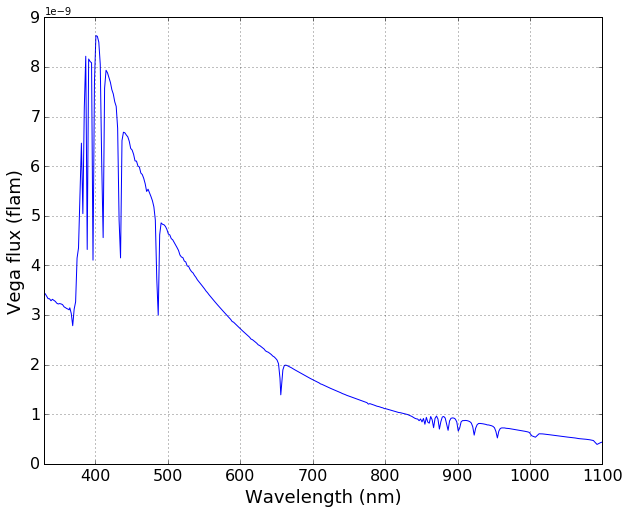
\includegraphics[width=0.5\textwidth]{Vega.png}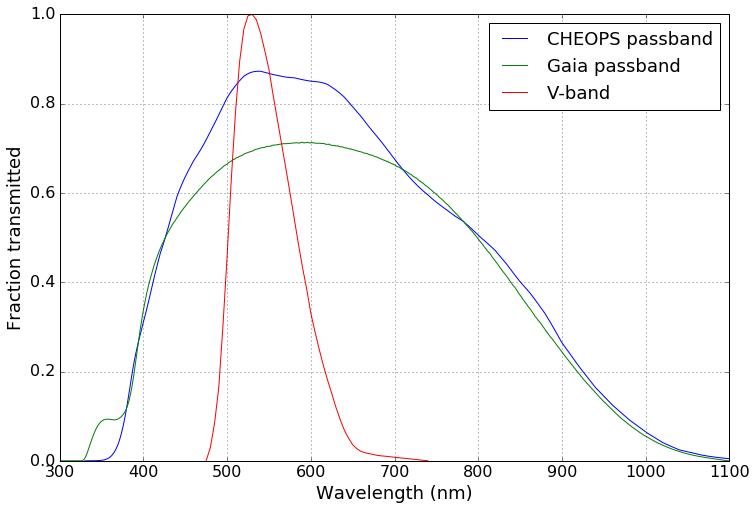
\includegraphics[width=0.5\textwidth]{passbands_May2020.png}
    \caption{Left: flux spectrum of Vega. Right: Gaia passband and V-band transmission curves, with the CHEOPS global throughput shown for comparison.}
    \label{fig:fluxnorm}
  \end{center}
\end{figure}

\begin{equation}
photonflux_{mag0.035}(\lambda) = photonflux(\lambda)\frac{\int photonflux_{Vega}(\lambda) \times transmission_{refBand}(\lambda)}{\int photonflux(\lambda) \times transmission_{refBand}(\lambda)}
\label{eq:fluxnorm}
\end{equation}

Finally, the flux spectrum of each star is renormalized according to the value of input magnitude using equation~\ref{eq:mag}.

\begin{equation}
photonflux(\lambda) = photonflux_{mag0.035}(\lambda) \times 10^{-0.4 (magnitude-0.035)}
\label{eq:mag}
\end{equation}

The above calculations are performed with a wavelength resolution of 1~nm over the range 330nm to 1100nm. Photon flux spectra normalised to V-band magnitude 9 are shown for a selection of spectral types in Figure~\ref{fig:seds}, comparing SED spectra with black body for the same effective temperature.

\begin{figure}[hbtp]
  \begin{center}
    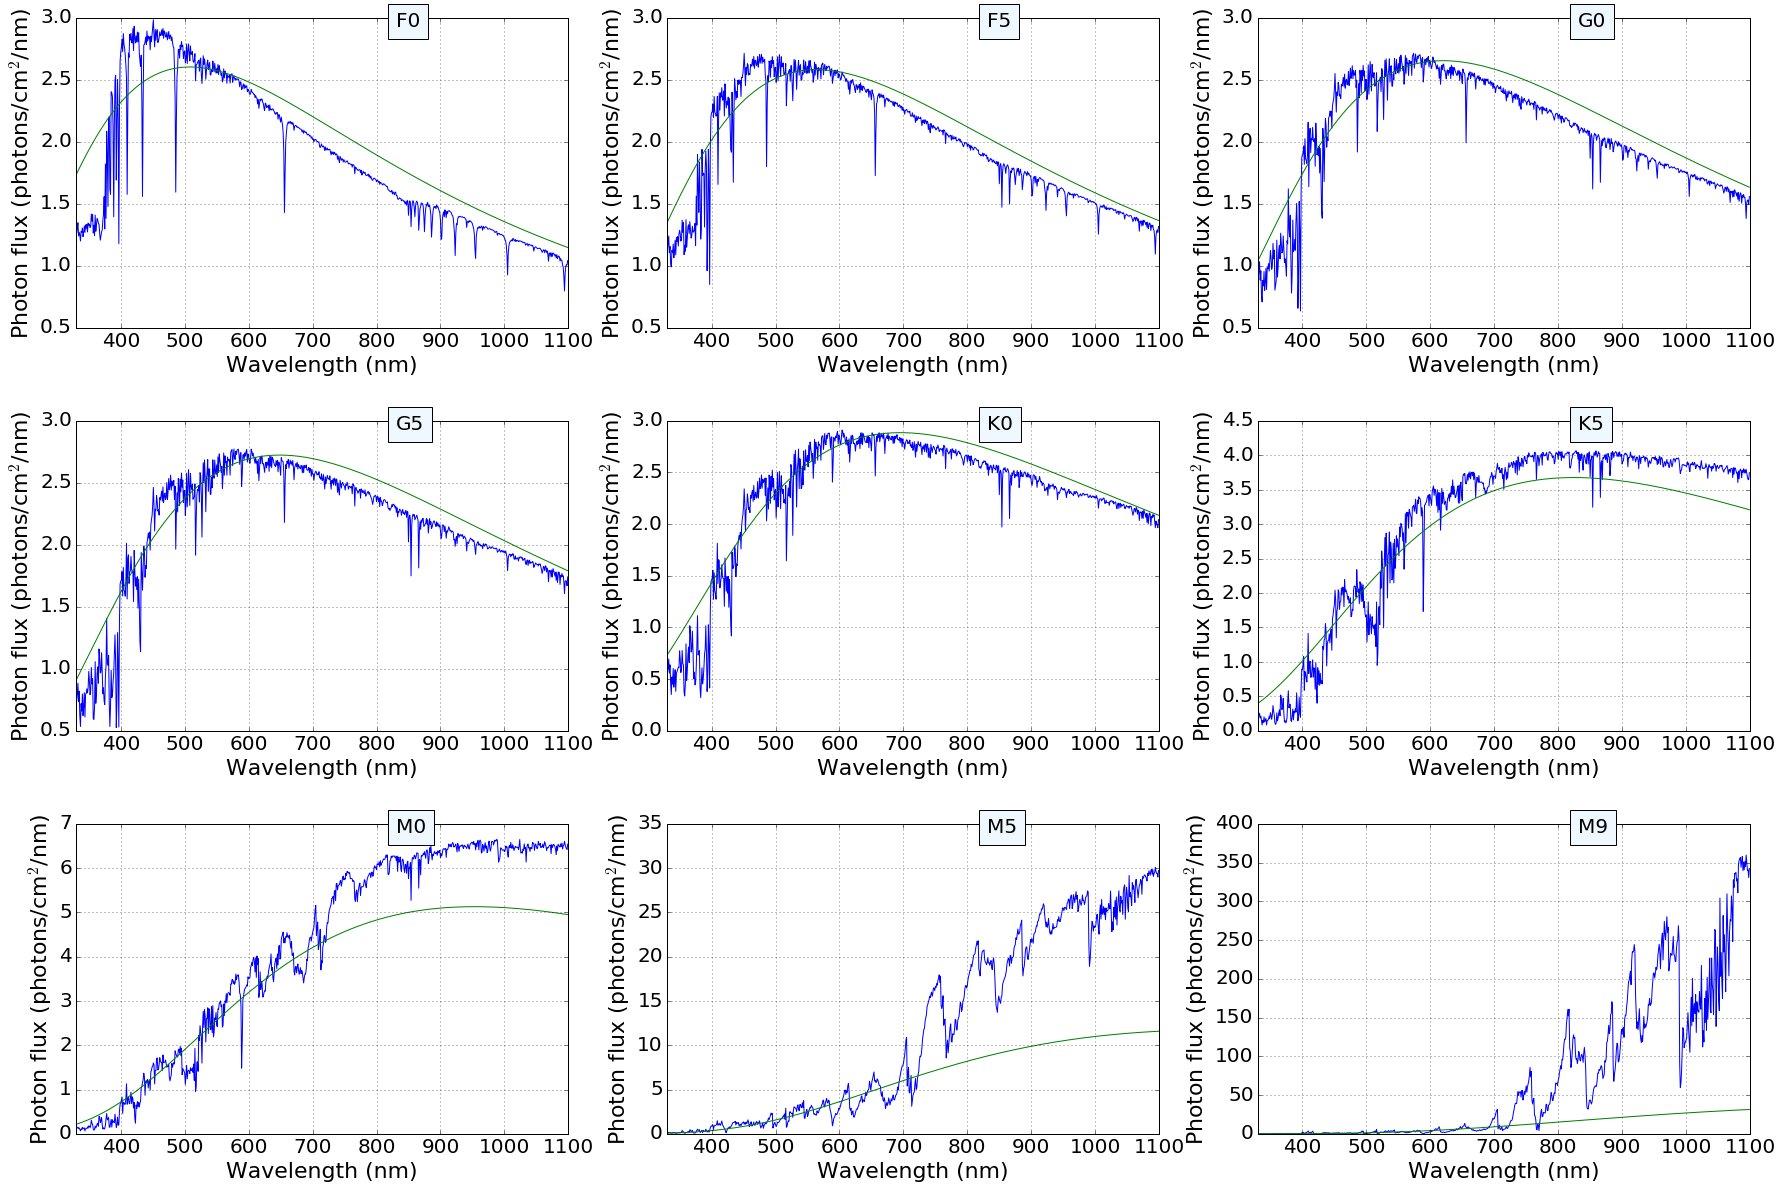
\includegraphics[width=\textwidth]{SEDs.png}
    \caption{Photon flux spectra normalised to V-band magnitude 9, for a selection of spectral types, for PHOENIX SED models (blue) and a Planck black body model (green). The normalisation is such that the integral is the same in the V-band (peaking at 500-600nm, see Figure~\ref{fig:fluxnorm}).}
    \label{fig:seds}
  \end{center}
\end{figure}

The filename providing the SEDs is the only input parameter for the flux calculation, defined in Table~\ref{tab:flux}.

\begin{table}[hb]
  \caption{Input parameters for stellar flux calculation}

  \htmlanchor{sedFilename}
  \begin{tabular}{| l | p{13cm} |}
    \hline 
    {\bf Parameter} & filename for Spectral Energy Distributions\\
    {\bf Unit} & \\
    {\bf Type / Format} & \href{https://htmlpreview.github.io/?https://github.com/davefutyan/common_sw/blob/master/doc/fits_data_model/REF_APP_SEDTeff.html}{REF\_APP\_SEDTeff}\\
    {\bf Default value} & \href{https://github.com/davefutyan/CHEOPSim/releases/tag/v1.0}{CH\_TU2015-01-01T00-00-00\_REF\_APP\_SEDTeff\_V0102.fits}\\
    {\bf Comments} & If the value does not contain the substring REF\_APP\_SEDTeff, a black body spectrum is generated\\
    \hline
  \end{tabular}
  \bigskip 

  \htmlanchor{gaiaBand}
  \begin{tabular}{| l | p{13cm} |}
    \hline 
    {\bf Parameter} & Flag to indicate whether to use the Gaia band or the V-band for stellar flux normalization\\
    {\bf Unit} & \\
    {\bf Type / Format} & boolean\\
    {\bf Default value} & true\\
    {\bf Comments} & \\
    \hline
  \end{tabular}
  \bigskip
  
  \label{tab:flux}
\end{table}

\clearpage

\htmlanchor{TransitFluxModulator}
\subsection{Transit Model:  {\it TransitFluxModulator}}
\label{sec:TransitFluxModulator}

This module can be run separately with different parameters, for any of the first 3 stars in the list defined in StarProducer (Section~\ref{sec:StarProducer}), indicated as ``target star'', ``background star 1'' and ``background star 2'' in the web interface. Running the module for background stars allows the possibility to simulate a background star undergoing a transit-like variation (e.g. eclipsing binary) which could affect the extracted light curve for the target star. By default, the module is run for the target star only.

The transit curve is calculated as described by Mandel and Agol~\cite{MandelAgol}.  Without limb darkening, the transit curve is entirely defined by a two parameters: the time independent parameter $p$, defined as the ratio of the planet radius to the star radius, and the time dependent parameter $z(t)$, defined as the separation between the star and the planet centres divided by stellar radius, $R_{star}$.  These two parameters are derived from the input information in Table~\ref{tab:transit} together with the mass and radius of the star, which depend on the spectral type as indicated in Tables~\ref{tab:starProperties1} and \ref{tab:starProperties2}, with $z(t)$ calculated according to equation~\ref{eq:transit1}.

\begin{equation}
z(t)=\sqrt{\left(\frac{a}{R_{star}}sin(2\pi f(t))\right)^2 + (b\cos(2\pi f(t)))^2}
\label{eq:transit1}
\end{equation}
where $b$ is the impact parameter, $f(t)$ is the difference between the current time $t$ and the transit midpoint time as a fraction of the orbit period, and $a$ is the semi-major axis of the planets' orbit, given by $a=\sqrt[3]{G M_{star}/\left(2\pi/P\right)^2}$, where $M_{star}$ is the mass of the star and $P$ is the orbit period.

Given $p$ and $z(t)$, the multiplication factor to be applied to the flux as a function of time is calculated as $F_{transit}(t)=1-\lambda^e(p,z(t))$, where $\lambda^e(p,z(t))$ is given by:

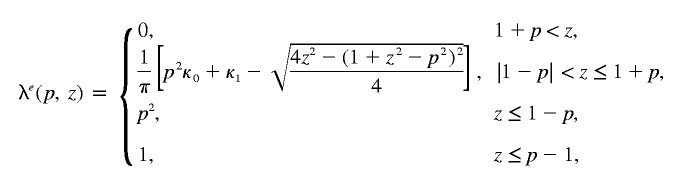
\includegraphics[width=0.8\textwidth]{transitEquation.png}

where $\kappa_0=\cos^{-1}[(p^2+z^2-1)/2pz]$ and $\kappa_1=\cos^{-1}[(1-p^2+z^2)/2z]$

\begin{table}[hb]
  \caption{Input parameters required to define the transit curve for a given star}

  \htmlanchor{firstTransitTime}
  \begin{tabular}{| l | p{13cm} |}
    \hline 
    {\bf Parameter} & Time of midpoint of first transit as a fraction of the simulation duration\\
    {\bf Unit} & \\
    {\bf Type / Format} & double\\
    {\bf Default value} & 0.5\\
    {\bf Comments} & \\
    \hline
  \end{tabular}
  \bigskip

  \htmlanchor{planetRadius}
  \begin{tabular}{| l | p{13cm} |}
    \hline 
    {\bf Parameter} & Planet radius\\
    {\bf Unit} & Jupiter, Neptune or Earth radii\\
    {\bf Type / Format} & double\\
    {\bf Default value} & 1.0 Neptune radii\\
    {\bf Comments} & In the web interface, the choice of units (Jupiter, Neptune or Earth radii) is specified via a drop down menu.  In the xml file, this choice is specified via an additional parameter {\it planetScale} which takes the form of a string with value ``Jupiter'' ``Neptune'', or ``Earth''. Values assumed for Jupiter, Neptune and Earth radii are 69911km, 24622km and 6371km, respectively.\\
    \hline
  \end{tabular}
  \bigskip

  \htmlanchor{orbitPeriod}
  \begin{tabular}{| l | p{13cm} |}
    \hline 
    {\bf Parameter} & Planet orbit period around the star\\
    {\bf Unit} & hours or days\\
    {\bf Type / Format} & double\\
    {\bf Default value} & 2.0 days\\
    {\bf Comments} & In the web interface, the choice of units (hours or days) is specified via a drop down menu.  In the xml file, this choice is specified via an additional parameter {\it orbitUnits} which takes the form of a string with value ``hours'' or ``days''\\
    \hline
  \end{tabular}
  \bigskip

  \htmlanchor{impactParameter}
  \begin{tabular}{| l | p{13cm} |}
    \hline 
    {\bf Parameter} & Impact parameter for the transit\\
    {\bf Unit} & dimensionless\\
    {\bf Type / Format} & double\\
    {\bf Default value} & 0.0\\
    {\bf Comments} & Smallest distance from planet centre to star centre divided by star radius\\
    \hline
  \end{tabular}
  \bigskip

  \label{tab:transit}
\end{table}

\clearpage 
\htmlanchor{limbDarkening}
\subsubsection{Limb Darkening}

Limb darkening is implemented according to the equations for quadratic limb darkening in Section 4 of~\cite{MandelAgol}.  The code has been implemented by converting C code written by Laura Kreidberg, made available by Eric Agol~\cite{AgolCode}, to C++.  The quadratic limb darkening formulae require two coefficients, whose values are assigned according to the spectral type as indicated in Tables~\ref{tab:limb1} and ~\ref{tab:limb2}. The coefficients have been calculated using the code provided by Espinoza \& Jordan~\cite{limbDarkening_code}, which implements the algorithms described in~\cite{limbDarkening}. The parameters used as input for the calculation of the coefficients are indicated in Table~\ref{tab:limb_inputs}.

\begin{table}[hbtp]
  \begin{center}
  \caption{Input parameters for the Espinoza \& Jordan algorithm~\cite{limbDarkening_code} used to calculate the limb darkening coefficients.}
  \begin{tabular}{| l | p{13cm} |}
    \hline 
    Input parameter & Value\\
    \hline
Effective temperature & Defined separately for each spectral type - see Tables~\ref{tab:limb1} and ~\ref{tab:limb2}\\
Surface gravity & Defined separately for each spectral type - see Tables~\ref{tab:limb1} and ~\ref{tab:limb2}\\
Metallicity (M/H) & 0.0\\
Microturbulent velocity & 2 km/s\\
Response Function & Product of optical throughput and quantum efficiency as a function of wavelength, as defined in Section~\ref{sec:GlobalThroughputGenerator}, Figure~\ref{fig:throughput_qe}\\
Wavelength passband & 330-1100nm\\
Fitting Technique & ATLAS models interpolating 100 mu-points with a cubic spline~\cite{claret_bloeman}\\
    \hline
  \end{tabular}
  \label{tab:limb_inputs}
  \end{center}
\end{table}

\begin{table}[hbtp]
  \begin{center}
  \caption{Values for effective temperature, and surface gravity $g=g_{\odot}m/r^2$, where $m$ is the stellar mass in multiples of $M_{\odot}$ and $r$ is the stellar radius in multiples of $R_{\odot}$, and $g_{\odot}$ is the surface gravity of the Sun, used as input for the calculation of the limb darkening coefficients, together with the values of the calculated coefficients, for spectral types O7 to F9. Values for $m$ and $r$ are taken from ~\cite{stellarParameters}, and the value log($g_{\odot}$) = 4.43812 is taken from https://sites.google.com/site/mamajeksstarnotes/basic-astronomical-data-for-the-sun. The effective temperatures for the hottest stars are fixed by the algorithm~\cite{limbDarkening_code}.}
  \begin{tabular}{| c | c | c | c | c |}
    \hline 
    Spectral type & $T_{eff}$ (Kelvin) & log($g$) & coefficient 1 & coefficient 2\\
    \hline
O7 & 8750.0 & 4.0 & 0.286520868317 & 0.308907700487 \\
O8 & 8750.0 & 4.0 & 0.286520868317 & 0.308907700487 \\
O9 & 8750.0 & 4.0 & 0.286520868317 & 0.308907700487 \\
B0 & 8750.0 & 4.0 & 0.286520868317 & 0.308907700487 \\
B1 & 8750.0 & 4.0 & 0.286520868317 & 0.308907700487 \\
B2 & 8750.0 & 4.0 & 0.286520868317 & 0.308907700487 \\
B3 & 8750.0 & 4.0 & 0.286520868317 & 0.308907700487 \\
B4 & 8750.0 & 4.0 & 0.286520868317 & 0.308907700487 \\
B5 & 8750.0 & 4.0 & 0.286520868317 & 0.308907700487 \\
B6 & 8750.0 & 4.0 & 0.286520868317 & 0.308907700487 \\
B7 & 8750.0 & 4.0 & 0.286520868317 & 0.308907700487 \\
B8 & 8750.0 & 4.0 & 0.286520868317 & 0.308907700487 \\
B9 & 8750.0 & 4.0 & 0.286520868317 & 0.308907700487 \\
A0 & 8750.0 & 4.0 & 0.286520868317 & 0.308907700487 \\
A1 & 8750.0 & 4.0 & 0.286520868317 & 0.308907700487 \\
A2 & 8750.0 & 4.0 & 0.286520868317 & 0.308907700487 \\
A3 & 8500.0 & 4.0 & 0.306253269964 & 0.30321814101 \\
A4 & 8250.0 & 4.0 & 0.313824482577 & 0.307665491901 \\
A5 & 8000.0 & 4.0 & 0.295125157409 & 0.324758309659 \\
A6 & 8000.0 & 4.0 & 0.295125157409 & 0.324758309659 \\
A7 & 7750.0 & 4.0 & 0.275061199017 & 0.333009936736 \\
A8 & 7500.0 & 4.0 & 0.256990075135 & 0.344430500701 \\
A9 & 7500.0 & 4.0 & 0.256990075135 & 0.344430500701 \\
F0 & 7250.0 & 4.0 & 0.269785263303 & 0.33890660747 \\
F1 & 7000.0 & 4.0 & 0.288081047361 & 0.328380696599 \\
F2 & 6750.0 & 4.0 & 0.306357595627 & 0.317520397667 \\
F3 & 6750.0 & 4.0 & 0.306357595627 & 0.317520397667 \\
F4 & 6750.0 & 4.0 & 0.306357595627 & 0.317520397667 \\
F5 & 6500.0 & 4.0 & 0.326391697018 & 0.30664289583 \\
F6 & 6250.0 & 4.5 & 0.351549542553 & 0.295645429168 \\
F7 & 6250.0 & 4.5 & 0.351549542553 & 0.295645429168 \\
F8 & 6250.0 & 4.5 & 0.351549542553 & 0.295645429168 \\
F9 & 6000.0 & 4.5 & 0.384920992243 & 0.277093128668 \\
    \hline
  \end{tabular}
  \label{tab:limb1}
  \end{center}
\end{table}

\begin{table}[hbtp]
  \begin{center}
  \caption{Values for effective temperature, and surface gravity $g=g_{\odot}m/r^2$, where $m$ is the stellar mass in multiples of $M_{\odot}$ and $r$ is the stellar radius in multiples of $R_{\odot}$, and $g_{\odot}$ is the surface gravity of the Sun, used as input for the calculation of the limb darkening coefficients, together with the values of the calculated coefficients, for spectral types G0 to M9. Values for $m$ and $r$ are taken from ~\cite{stellarParameters}, and the value log($g_{\odot}$) = 4.43812 is taken from https://sites.google.com/site/mamajeksstarnotes/basic-astronomical-data-for-the-sun. The effective temperatures for the coolest stars are fixed by the algorithm~\cite{limbDarkening_code}.}
  \begin{tabular}{| c | c | c | c | c |}
    \hline 
    Spectral type & $T_{eff}$ (Kelvin) & log($g$) & coefficient 1 & coefficient 2\\
    \hline
G0 & 6000.0 & 4.5 & 0.384920992243 & 0.277093128668 \\
G1 & 6000.0 & 4.5 & 0.384920992243 & 0.277093128668 \\
G2 & 5750.0 & 4.5 & 0.426558788278 & 0.251124432854 \\
G3 & 5750.0 & 4.5 & 0.426558788278 & 0.251124432854 \\
G4 & 5750.0 & 4.5 & 0.426558788278 & 0.251124432854 \\
G5 & 5750.0 & 4.5 & 0.426558788278 & 0.251124432854 \\
G6 & 5500.0 & 4.5 & 0.471489816141 & 0.221145118953 \\
G7 & 5500.0 & 4.5 & 0.471489816141 & 0.221145118953 \\
G8 & 5500.0 & 4.5 & 0.471489816141 & 0.221145118953 \\
G9 & 5250.0 & 4.5 & 0.52086069776 & 0.186011230377 \\
K0 & 5250.0 & 4.5 & 0.52086069776 & 0.186011230377 \\
K1 & 5250.0 & 4.5 & 0.52086069776 & 0.186011230377 \\
K2 & 5000.0 & 4.5 & 0.571938795431 & 0.146705365271 \\
K3 & 4750.0 & 4.5 & 0.618702860724 & 0.108414083672 \\
K4 & 4500.0 & 4.5 & 0.656870172111 & 0.0776856531504 \\
K5 & 4500.0 & 4.5 & 0.656870172111 & 0.0776856531504 \\
K6 & 4250.0 & 4.5 & 0.641346757351 & 0.0942836350409 \\
K7 & 4000.0 & 4.5 & 0.500461094367 & 0.212829785288 \\
K8 & 4000.0 & 4.5 & 0.500461094367 & 0.212829785288 \\
K9 & 4000.0 & 4.5 & 0.500461094367 & 0.212829785288 \\
M0 & 3750.0 & 4.5 & 0.369553033549 & 0.323362461751 \\
M1 & 3750.0 & 5.0 & 0.268878243523 & 0.399987999316 \\
M2 & 3500.0 & 5.0 & 0.290655602581 & 0.392227307466 \\
M3 & 3500.0 & 5.0 & 0.290655602581 & 0.392227307466 \\
M4 & 3500.0 & 5.0 & 0.290655602581 & 0.392227307466 \\
M5 & 3500.0 & 5.0 & 0.290655602581 & 0.392227307466 \\
M6 & 3500.0 & 5.0 & 0.290655602581 & 0.392227307466 \\
M7 & 3500.0 & 5.0 & 0.290655602581 & 0.392227307466 \\
M8 & 3500.0 & 5.0 & 0.290655602581 & 0.392227307466 \\
M9 & 3500.0 & 5.0 & 0.290655602581 & 0.392227307466 \\
    \hline
  \end{tabular}
  \label{tab:limb2}
  \end{center}
\end{table}

Light curves calculated using the {\it TransitFluxModulator} module with default parameters are shown for each spectral type in Figures~\ref{fig:incidentLightCurve1} and \ref{fig:incidentLightCurve2}.

The module outputs a vector storing the multiplication factor to be applied to the flux for each time step of the simulation.

\begin{figure}[hbtp]
  \begin{center}
    {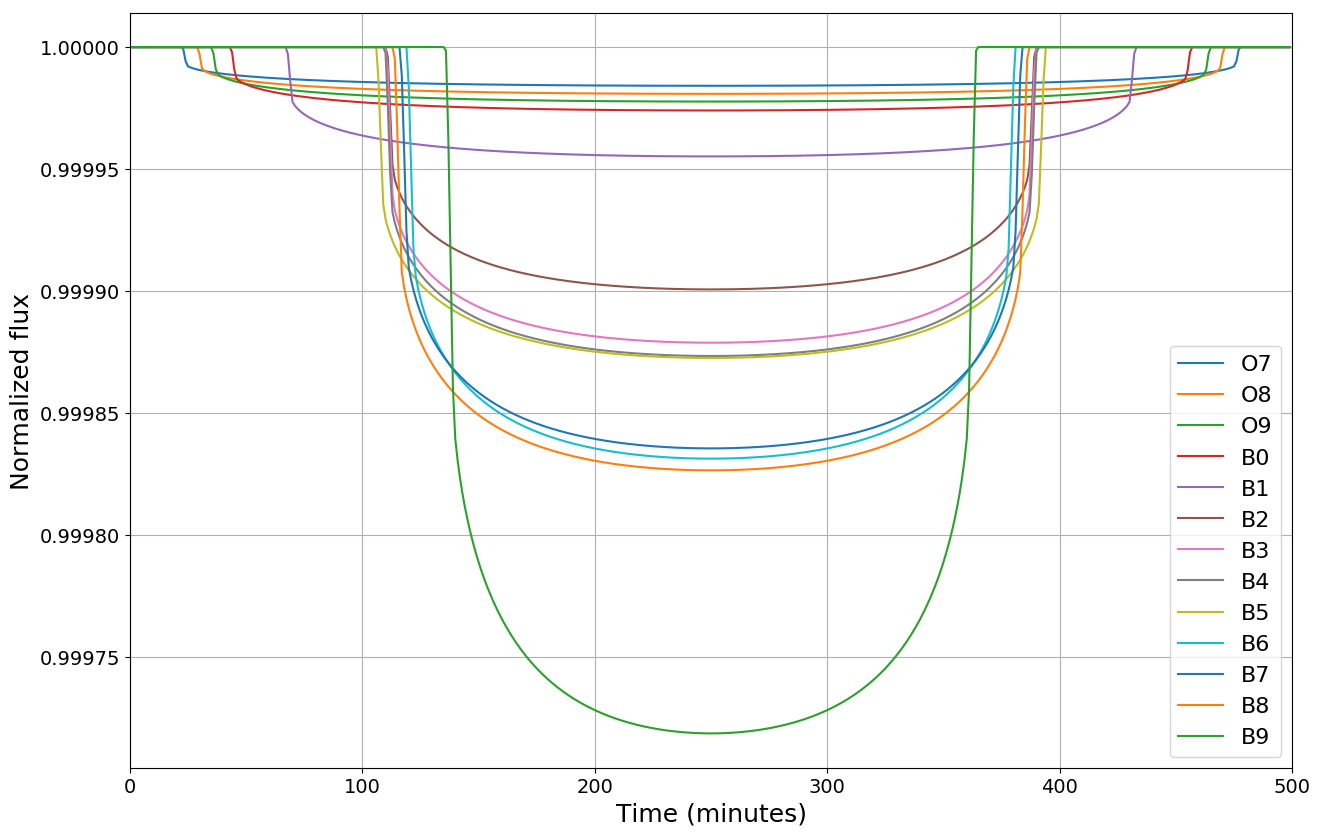
\includegraphics[width=0.8\textwidth]{limbDarkening_OB.png}}
    {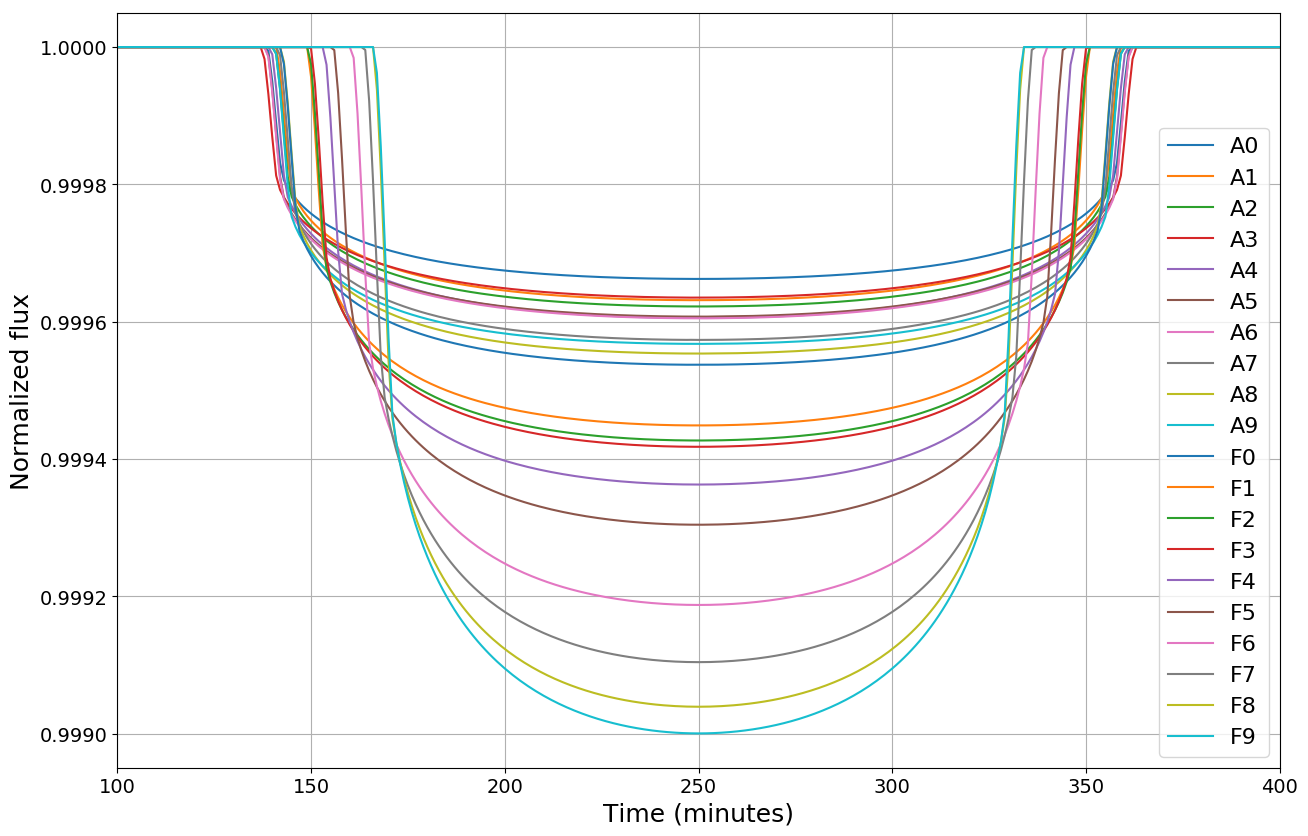
\includegraphics[width=0.8\textwidth]{limbDarkening_AF.png}}
    \caption{Transit light curves obtained using the default parameter values defined in Table~\ref{tab:transit} (Neptune with orbit period 2 days and zero impact parameter), for spectral types from O7 to F9.}
    \label{fig:incidentLightCurve1}
  \end{center}
\end{figure}

\begin{figure}[hbtp]
  \begin{center}
    {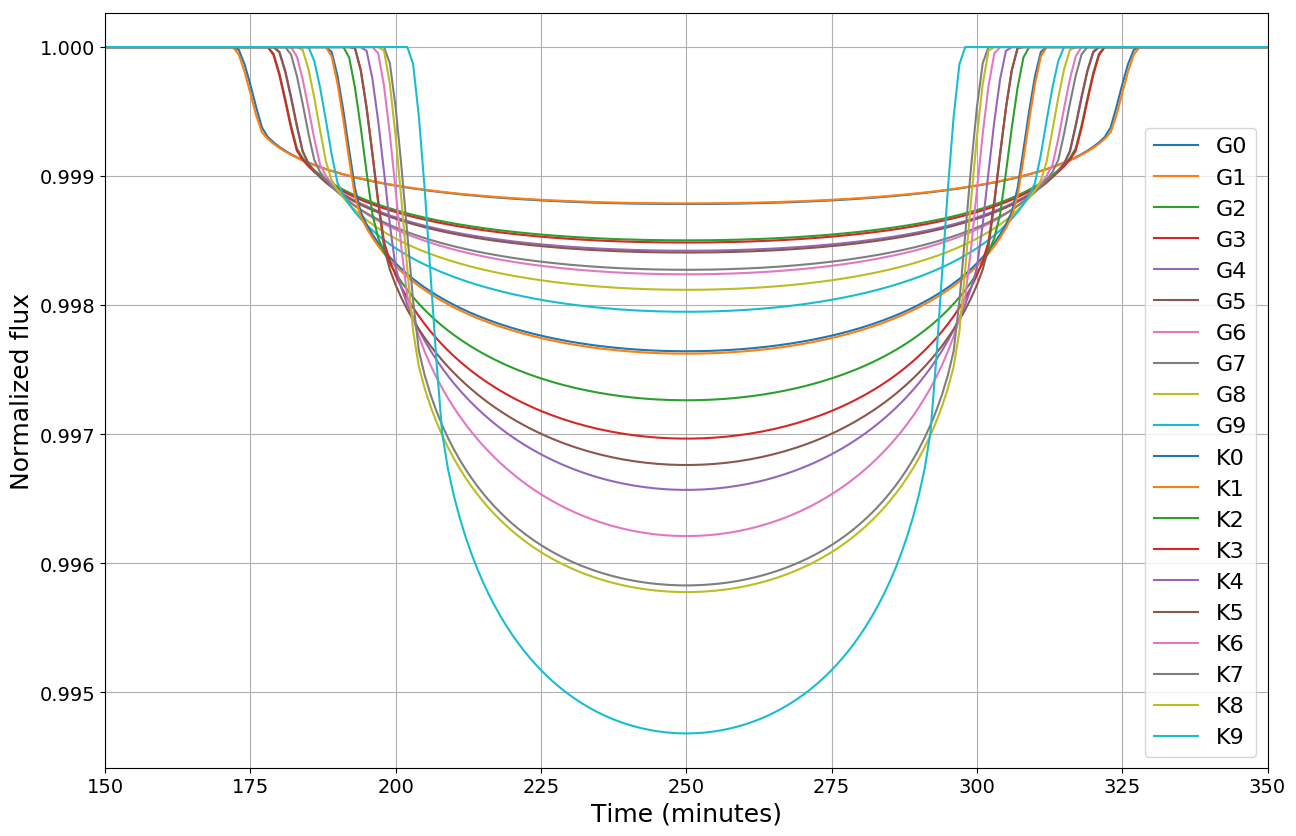
\includegraphics[width=0.8\textwidth]{limbDarkening_GK.png}}
    {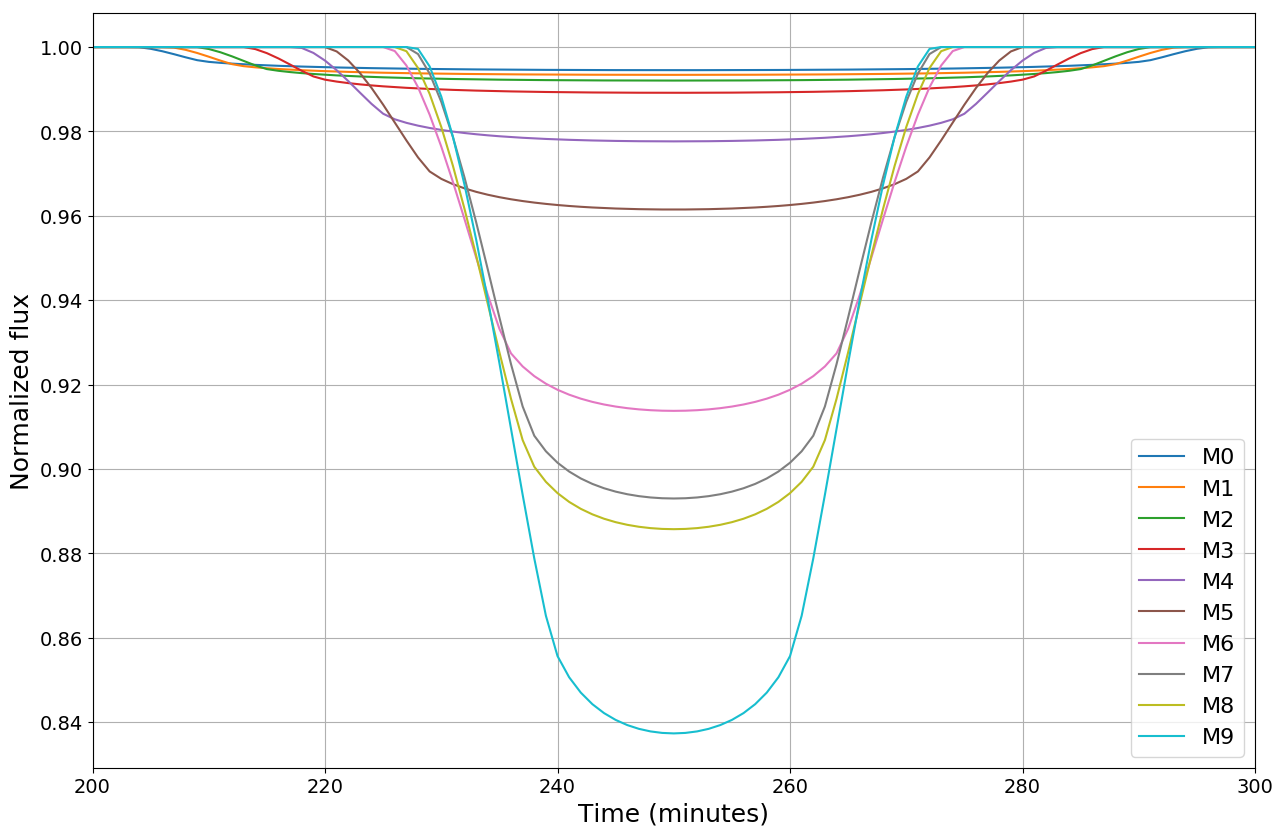
\includegraphics[width=0.8\textwidth]{limbDarkening_M.png}}
    \caption{Transit light curves obtained using the default parameter values defined in Table~\ref{tab:transit} (Neptune with orbit period 2 days and zero impact parameter), for spectral types from G0 to M9.}
    \label{fig:incidentLightCurve2}
  \end{center}
\end{figure}

\clearpage 
\htmlanchor{StellarNoiseFluxModulator}
\subsection{Stellar Noise:  {\it StellarNoiseFluxModulator}}
\label{sec:StellarNoiseFluxModulator}

Intrinsic stellar noise due to stellar granulation is modelled outside CHEOPSim~\cite{granularity}. CHEOPSim takes as input a set of 48 hour time series, each containing deviations from the normalized stellar flux due to granulation in steps of 15 seconds. Such time series have been generated for several values of each of the following parameters:
\begin{itemize}
\item the mass of the star
\item the radius of the star
\item the effective temperature of the star
\end{itemize}

Given the spectral type of the target star, defined by the user in the {\it StarProducer} module (Section~\ref{sec:StarProducer}), the time series used is that for which the above parameters match most closely to the parameters corresponding to the target star spectral type as defined in Tables~\ref{tab:starProperties1} and \ref{tab:starProperties2}. The input time series corresponding to 14 of the 30 spectral types are shown in Figure~\ref{fig:granulation}. The mass, radius and effective temperature parameter values corresponding to each time series are indicated in Table~\ref{tab:granulation_params}. For simulations longer than 48 hours, the time series is repeated.

The module outputs a vector storing the multiplication factor to be applied to the flux for each time step of the simulation.

The module cannot be run for spectral types hotter than F0 because the model does not apply to such stars since they have radiative rather than convective envelopes.

\begin{figure}[hbtp]
  \begin{center}
    \ifpdf
    {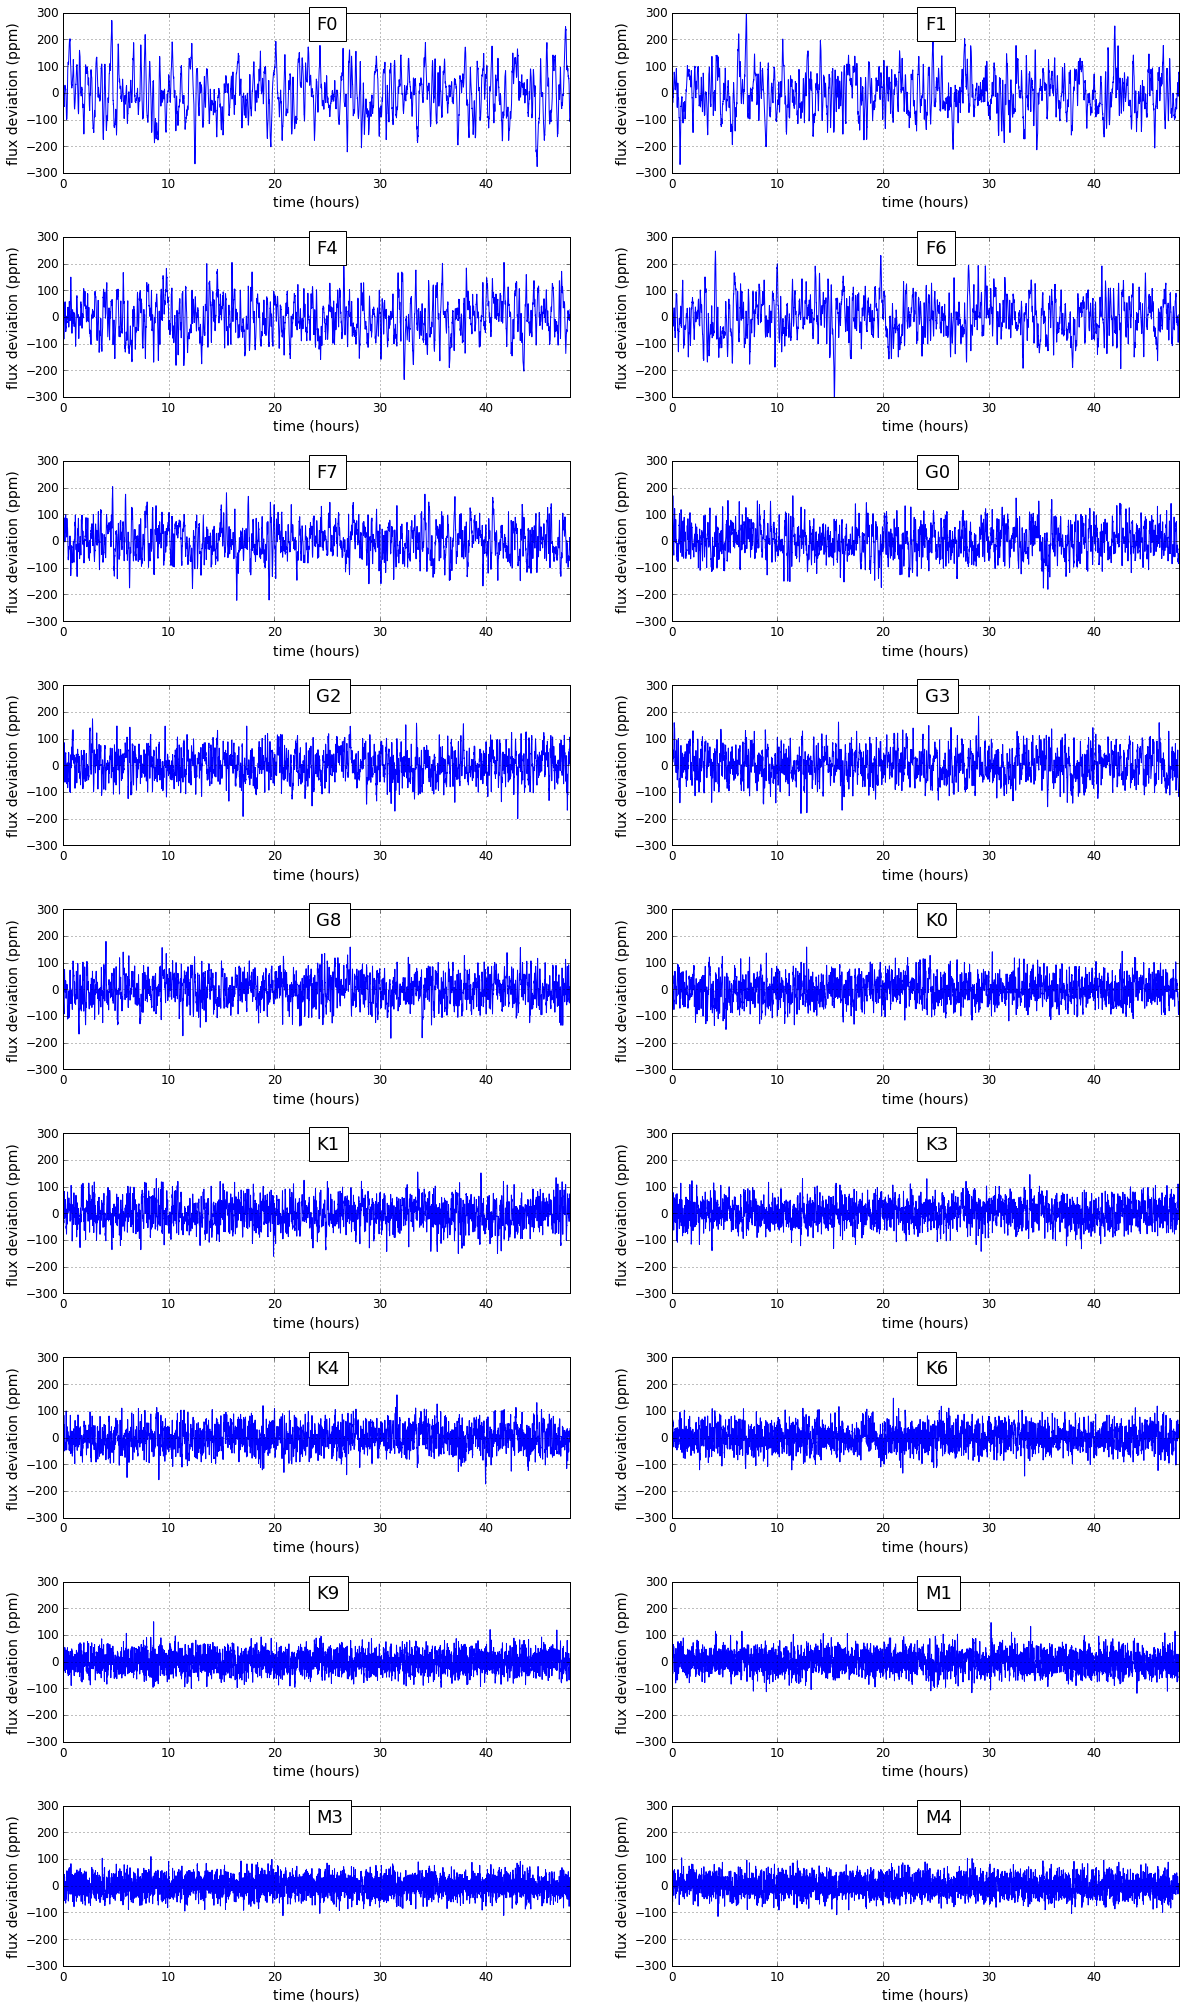
\includegraphics[width=0.8\textwidth]{granulation_kallinger_Jul2018.png}}
    \else
    {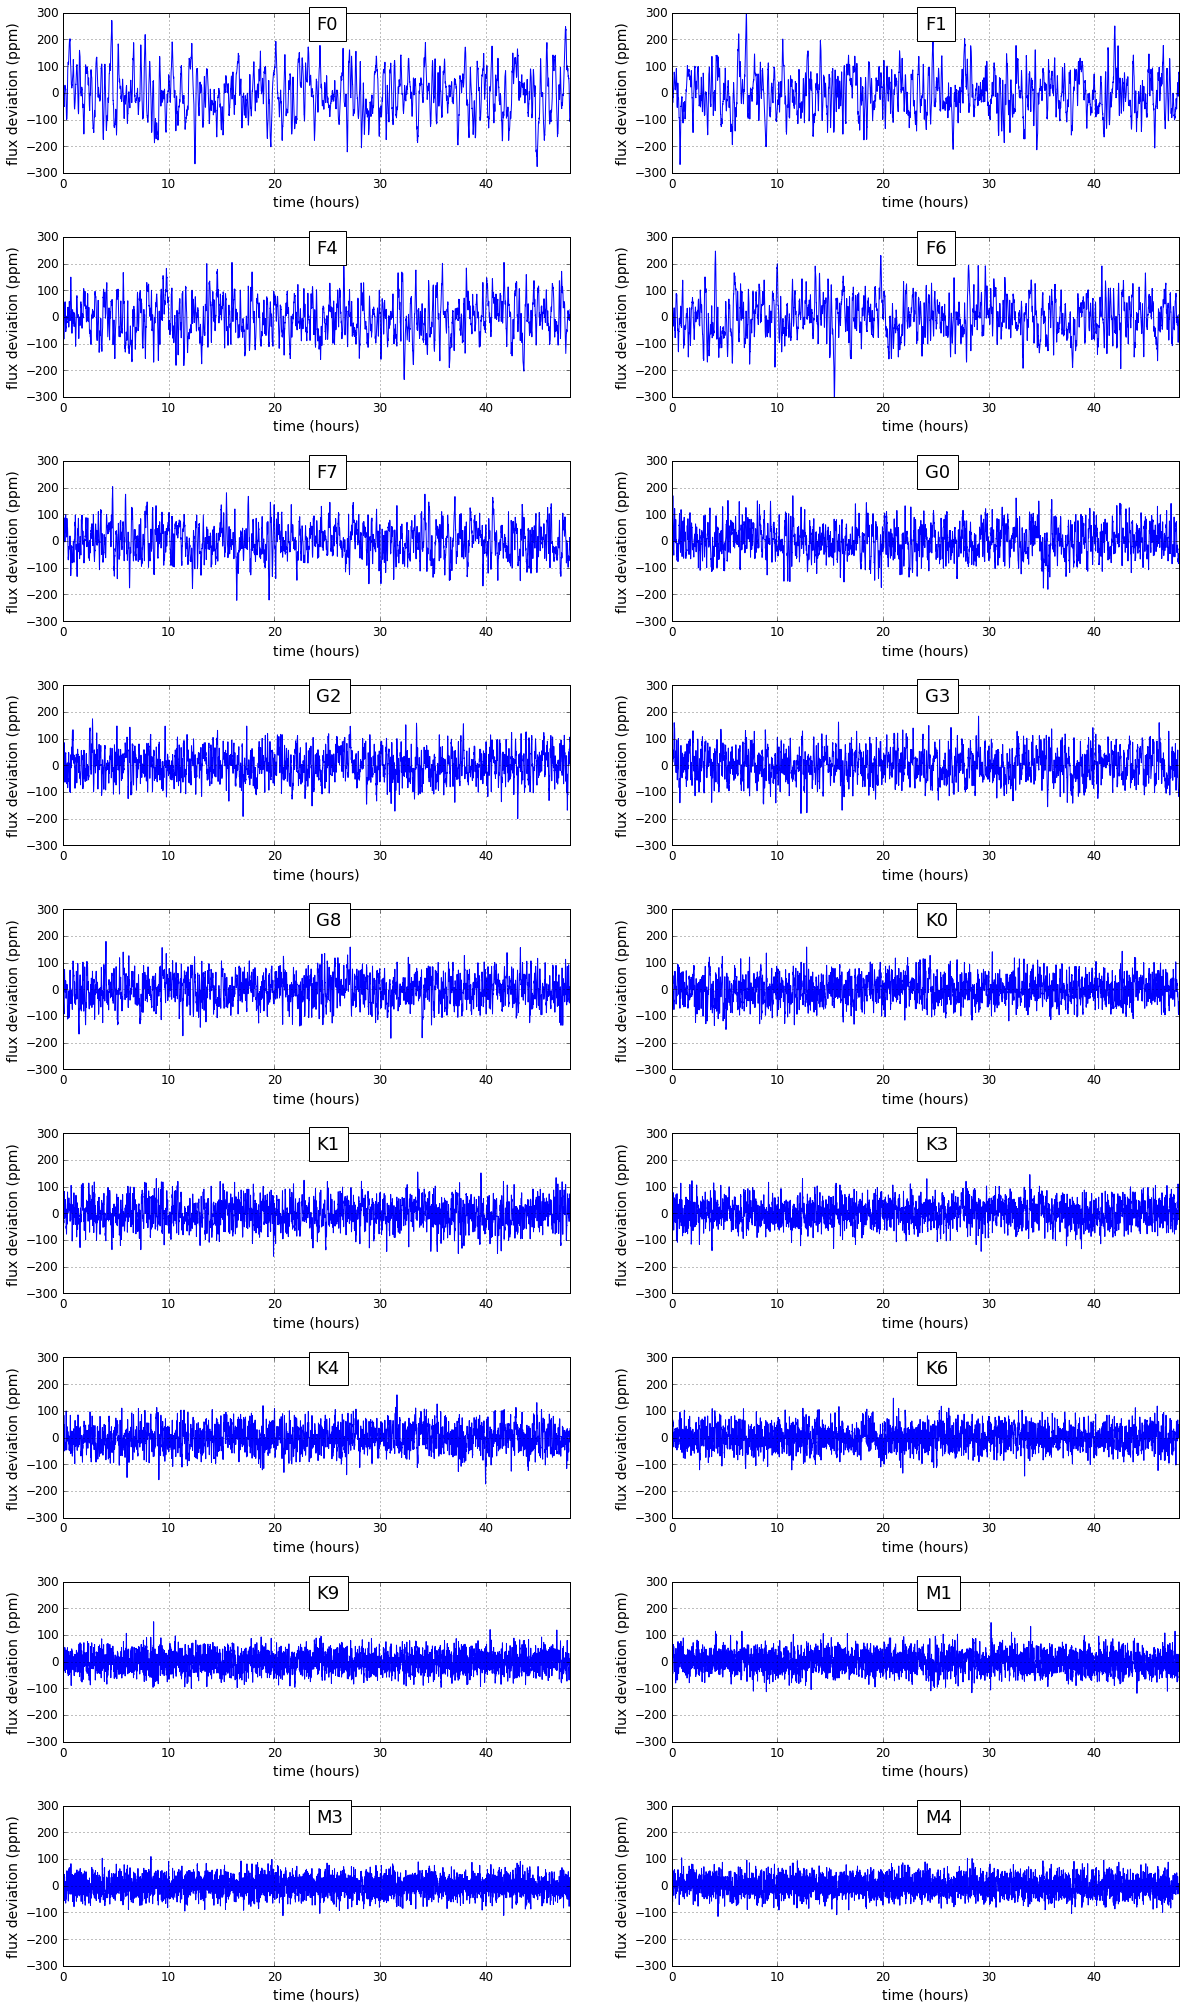
\includegraphics[width=\textwidth]{granulation_kallinger_Jul2018.png}}
    \fi
    \caption{Time series showing fluctuations in stellar output due to granulation, in steps of 15 seconds, for a selection of spectral types.}
    \label{fig:granulation}
  \end{center}
\end{figure}

\begin{table}[hb]
  \begin{center}
  \caption{Effective temperature, stellar radius and stellar mass used to derive the granulation time series assigned to each spectral type.}
  \begin{tabular}{| c | c | c | c |}
    \hline 
    Spectral type & $T_{eff}$ (Kelvin) & mass ($M_{\odot}$) & radius ($R_{\odot}$)\\
    \hline
F0 & 6500 & 1.4 & 1.8 \\
F1 & 6500 & 1.4 & 1.6 \\
F2 & 6500 & 1.4 & 1.6 \\
F3 & 6500 & 1.4 & 1.6 \\
F4 & 6500 & 1.4 & 1.5 \\
F5 & 6500 & 1.4 & 1.5 \\
F6 & 6500 & 1.2 & 1.4 \\
F7 & 6000 & 1.2 & 1.2 \\
F8 & 6000 & 1.2 & 1.2 \\
F9 & 6000 & 1.2 & 1.2 \\
G0 & 6000 & 1.2 & 1.1 \\
G1 & 6000 & 1.2 & 1.1 \\
G2 & 6000 & 1.1 & 1.0 \\
G3 & 5500 & 1.0 & 1.0 \\
G4 & 5500 & 1.0 & 1.0 \\
G5 & 5500 & 1.0 & 1.0 \\
G6 & 5500 & 1.0 & 1.0 \\
G7 & 5500 & 1.0 & 1.0 \\
G8 & 5500 & 0.9 & 0.9 \\
G9 & 5500 & 0.9 & 0.9 \\
K0 & 5500 & 0.9 & 0.8 \\
K1 & 5000 & 0.8 & 0.8 \\
K2 & 5000 & 0.8 & 0.8 \\
K3 & 5000 & 0.8 & 0.7 \\
K4 & 4500 & 0.7 & 0.7 \\
K5 & 4500 & 0.7 & 0.7 \\
K6 & 4000 & 0.6 & 0.6 \\
K7 & 4000 & 0.6 & 0.6 \\
K8 & 4000 & 0.6 & 0.6 \\
K9 & 4000 & 0.6 & 0.5 \\
M0 & 4000 & 0.6 & 0.5 \\
M1 & 3500 & 0.5 & 0.5 \\
M2 & 3500 & 0.5 & 0.5 \\
M3 & 3500 & 0.4 & 0.4 \\
M4 & 3000 & 0.2 & 0.3 \\
M5 & 3000 & 0.2 & 0.3 \\
M6 & 3000 & 0.2 & 0.3 \\
M7 & 3000 & 0.2 & 0.3 \\
M8 & 3000 & 0.2 & 0.3 \\
M9 & 3000 & 0.2 & 0.3 \\
    \hline
  \end{tabular}
  \label{tab:granulation_params}
  \end{center}
\end{table}

\clearpage 
\htmlanchor{StellarVariationFluxModulator}
\subsection{Stellar Variation:  {\it StellarVariationFluxModulator}}
\label{sec:StellarVariationFluxModulator}

This module simulates the flux modulation produced by stellar active regions (spots and plages) as they rotate in and out of view throughout the stellar rotational period.

The rotational modulation is modelled using a Gaussian process in time, with a quasi-periodic kernel function (see equation 5.16 in~\cite{variation}) that produces a covariance with a periodic behaviour modulated by a decay away from exact periodicity:
$$dt = t_i - t_j$$
$$k = A\cdot exp(-0.5dt^2/\tau^2 - 2\sin(\pi dt/P)^2/\mu^2) ,$$
where the four required parameters are the amplitude $A$ (in mmag), the decay time $\tau$, the stellar rotation period $P$, and the smoothing or structure parameter $\mu$.
The stellar rotation period is provided by the user, the amplitude and decay time are taken randomly from the sample generated in \cite{HelenGiles}, based on the spectral type of the target star, and the dimensionless structure parameter $\mu$ is randomly drawn between 0.5 and 1.0.

The module takes two parameters as input: the rotation period of the star and a seed for random number generation (Table~\ref{tab:variation}). The algorithm uses these inputs, together with the spectral type of the star, and the simulation duration in order to define a modulation curve. An example modulation curve with duration 20 days for a K4 star with rotation period 8.3 days is shown in Figure~\ref{fig:variation1}. Figure~\ref{fig:variation2} shows the same modulation curve combined with the output of the StellarNoiseFluxModulator and TransitFluxModulator modules, using their default settings. Figure~\ref{fig:variation2} shows a zoom on one of the transits.

The module outputs a vector storing the multiplication factor to be applied to the flux for each time step of the simulation.

The module cannot be run for spectral types hotter than F0V because the model does not apply to such stars since they have radiative rather than convective envelopes.

\begin{table}[hb]
  \caption{Input parameters required to define the stellar variation for a given star}

  \htmlanchor{rotationPeriod}
  \begin{tabular}{| l | p{13cm} |}
    \hline 
    {\bf Parameter} & Stellar rotation period\\
    {\bf Unit} & days\\
    {\bf Type / Format} & double\\
    {\bf Default value} & 5.0\\
    {\bf Comments} & \\
    \hline
  \end{tabular}
  \bigskip

  \htmlanchor{stellarVariationSeed}
  \begin{tabular}{| l | p{13cm} |}
    \hline 
    {\bf Parameter} & Seed for random number generation\\
    {\bf Unit} & \\
    {\bf Type / Format} & int\\
    {\bf Default value} & 1234\\
    {\bf Comments} & Using the same seed guarantees reproducibility only if the simulation duration, stellar rotation period and spectral type are also unchanged.\\
    \hline
  \end{tabular}
  \bigskip

  \label{tab:variation}
\end{table}

\begin{figure}[hbtp]
  \begin{center}
    {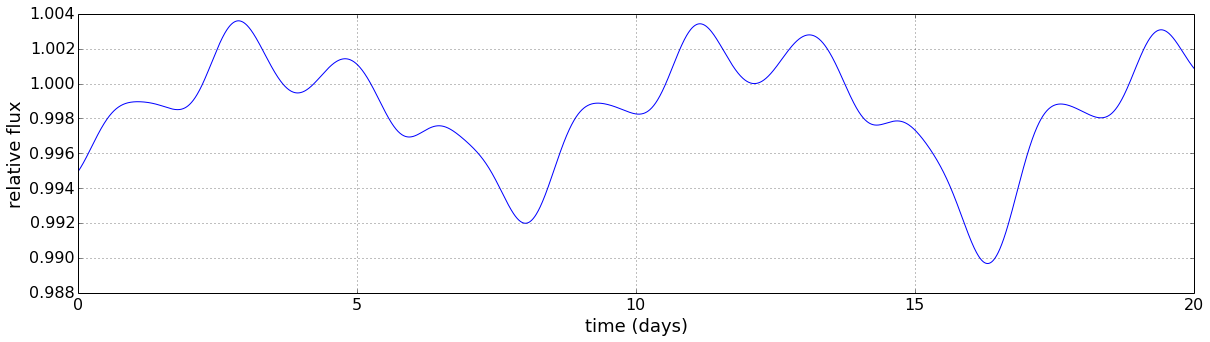
\includegraphics[width=\textwidth]{stellar_variation1.png}}
    \caption{Stellar variation modulation curve with 20 day duration for a K4 star with rotation period 8.3 days, using the default random seed.}
    \label{fig:variation1}
  \end{center}
\end{figure}

\begin{figure}[hbtp]
  \begin{center}
    {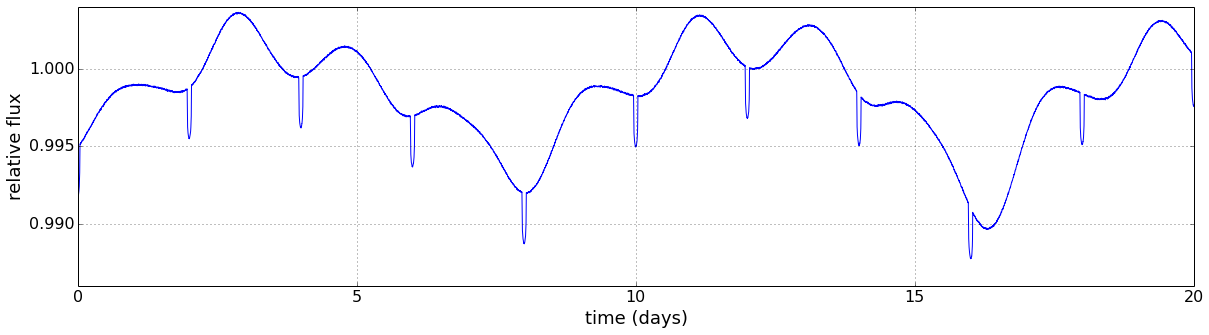
\includegraphics[width=\textwidth]{stellar_variation2.png}}
    \caption{Stellar variation modulation curve with 20 day duration for a K4 star with rotation period 8.3 days, using the default random seed, combined with the output of the StellarNoiseFluxModulator and TransitFluxModulator modules using their default settings.}
    \label{fig:variation2}
  \end{center}
\end{figure}

\begin{figure}[hbtp]
  \begin{center}
    {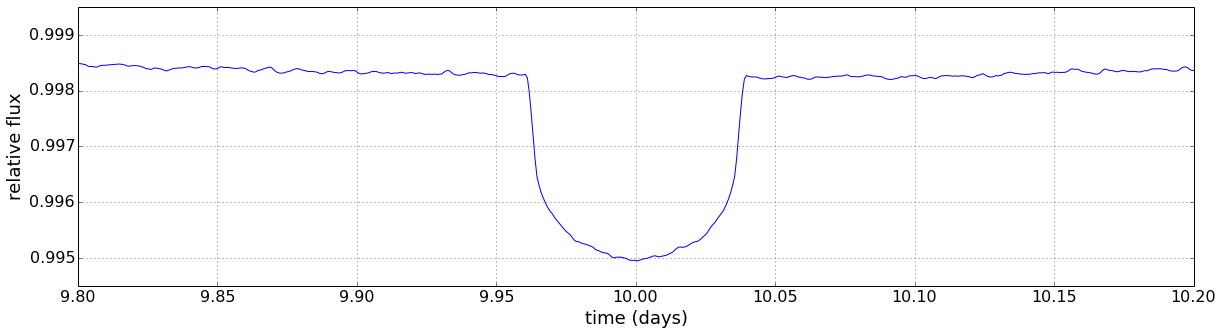
\includegraphics[width=\textwidth]{stellar_variation3.png}}
    \caption{Zoom on one of the transits in Figure~\ref{fig:variation2}.}
    \label{fig:variation3}
  \end{center}
\end{figure}

\clearpage 
\htmlanchor{UserFluxModifier}
\subsection{User Flux Fime Series:  {\it UserFluxModifier}}
\label{sec:UserFluxModifier}

This module allows the user to upload a file to define the flux time series of the target star. The time series must be provided as a plain ascii file containing two columns, as defined in Table~\ref{tab:userFluxFormat}.

\begin{table}[hb]
  \begin{center}
  \caption{Columns to be provided in the ascii file for the case of a stellar flux time series being uploaded by the user. The time series must be provided as a plain ascii file containing the columns indicated, separated by whitespace or tab. Note that there is a gap of 30s between the start of a visit and the start of the first exposure if there is no initial full frame image, and 35s plus the duration of one exposure if there is an initial full frame image. Rows for which the first character is \# are ignored.}
  \begin{tabular}{| l | c | c | l |}
    \hline
Column & Unit & Format & Notes\\
    \hline
Time & seconds & float & Number of seconds since the start of the visit\\
Flux relative to nominal & & float & Nominal flux = 1.0\\
    \hline
  \end{tabular}
  \label{tab:userFluxFormat}
\end{center}
\end{table}

\clearpage
\htmlanchor{ZodiacalLightGenerator}
\subsection{Zodiacal Light:  {\it ZodiacalLightGenerator}}
\label{sec:ZodiacalLightGenerator}

The flux from zodiacal light is added to the image uniformly across the exposed part of the CCD. The number of photons per pixel per second is calculated taking into account the wavelength dependence of the zodiacal light flux, and the angular separation between the pointing direction and the sun in ecliptic coordinates at the start date of the simulation.

The zodiacal light flux as a function of wavelength is taken from the WFC3 Instrument Handbook for the Hubble Space Telescope~\cite{HST_ETC}. The distribution is shown in Figure~\ref{fig:zodiacal_vs_wavelength} and the values used to calculate the wavelength integrated flux are shown in Table~\ref{tab:zodiacal_vs_wavelength}.

\begin{figure}[hbtp]
  \begin{center}
    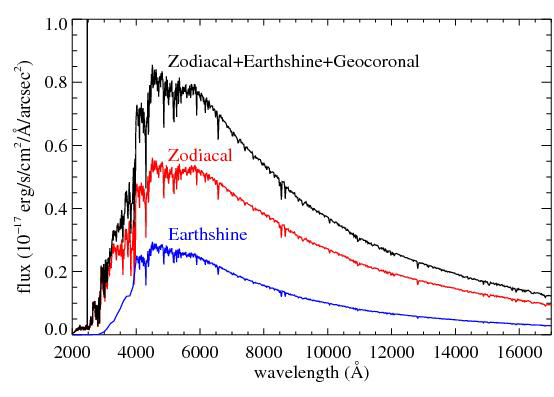
\includegraphics[width=0.5\textwidth]{zodiacal_vs_wavelength.png}
    \caption{Sky background intensity as a function of wavelength. The total sky spectrum (black) for the “high-background” case adopted in the WFC3 ETC, along with the individual contributions from zodiacal light and earth-shine. These data correspond to a V-band surface brightness of 22.1 mag arcsec$^{−2}$. The geocoronal emission line [O II] 2471 Å has a flux of $1.5\times10^{−15}$ erg cm$^{-2}$ s$^{-1}$ \AA$^{-1}$ arcsec$^{-2}$, extending beyond the upper limit of the plot.}
    \label{fig:zodiacal_vs_wavelength}
  \end{center}
\end{figure}

\begin{table}[hb]
  \begin{center}
  \caption{Sky background intensity, corresponding to a V-band surface brightness of 22.1 mag arcsec$^{−2}$, as a function of wavelength in 500\AA\ steps.}
  \begin{tabular}{|c|c|c|c|}
\hline
Wavelength & Earth-shine & Zodiacal light & Total sky background \\
(\AA) & (erg cm$^{-2}$ s$^{-1}$ \AA$^{-1}$ arcsec$^{-2}$) & (erg cm$^{-2}$ s$^{-1}$ \AA$^{-1}$ arcsec$^{-2}$) &(erg cm$^{-2}$ s$^{-1}$ \AA$^{-1}$ arcsec$^{-2}$) \\
\hline
4000 & 1.66E-18 & 3.12E-18 & 4.78E-18 \\
4500 & 2.59E-18 & 4.97E-18 & 7.57E-18 \\
5000 & 2.63E-18 & 5.07E-18 & 7.70E-18 \\
5500 & 2.55E-18 & 5.17E-18 & 7.72E-18 \\
6000 & 2.42E-18 & 5.14E-18 & 7.56E-18 \\
7000 & 1.95E-18 & 4.48E-18 & 6.42E-18 \\
8000 & 1.56E-18 & 3.82E-18 & 5.38E-18 \\
9000 & 1.23E-18 & 3.18E-18 & 4.40E-18 \\
10000 & 9.97E-19 & 2.70E-18 & 3.70E-18 \\
11000 & 8.02E-19 & 2.26E-18 & 3.06E-18 \\
\hline
  \end{tabular}
  \label{tab:zodiacal_vs_wavelength}
\end{center}
\end{table}

The wavelength integrated sky background photon flux, in photons per second per pixel (using the plate scale of 1 arcsecond per pixel), corresponding to a V-band surface brightness of 22.1 mag arcsec$^{−2}$, is calculated according to equation~\ref{eq:zodiacal_vs_wavelength}.

\begin{equation}
\label{eq:zodiacal_vs_wavelength}
photonflux_{skybackground}^{mag=22.1} = A_{telescope}\int_{3300\AA}^{11000\AA}{\frac{flux(\lambda)}{hc/\lambda}d\lambda} = 7.85728\ \mathrm{photons\ s^{-1} \ pixel^{-1}}
\end{equation}

where $A_{telescope}$ is the telescope collecting area (unobstructed circle with diameter 30cm), $flux(\lambda)$ is the zodiacal light flux at wavelength $\lambda$ taken from the third column of  Table~\ref{tab:zodiacal_vs_wavelength}, and $hc/\lambda$ is the energy of a photon with wavelength $\lambda$. The integral was calculated in 100$\AA$ steps, interpolating between the values in Table~\ref{tab:zodiacal_vs_wavelength}.

The photon flux from equation~\ref{eq:zodiacal_vs_wavelength} corresponds to a V-band surface brightness of 22.1 mag arcsec$^{−2}$. The brightness of the zodiacal sky background varies as a function of the angular separation between the pointing direction and the position of the sun in ecliptic polar coordinates as shown in Table~\ref{tab:zodiacal_vs_direction}, for which the values are taken from \cite{HST_ETC}.

\begin{table}[hb]
  \begin{center}
  \caption{Approximate zodiacal sky background, in V-mag per arcsec$^2$, as a function of the difference in ecliptic longitude and ecliptic latitude between the pointing direction and the position of the sun. SA stands for Solar Avoidance zone (pointing within 50 deg of the sun), where observations may not be made.}
  \begin{tabular}{|c|ccccccc|}
\hline
$\Delta$ Ecliptic & \multicolumn{7}{|c|}{$\Delta$ Ecliptic latitude (degrees)} \\
longitude & & & & & & & \\
(degrees) & 0 & 15 & 30 & 45 & 60 & 75 & 90 \\
\hline
0 & \textcolor{red}{SA} & \textcolor{red}{SA} & \textcolor{red}{SA} & \textcolor{red}{SA} & 22.6 & 23.0 & 23.3 \\
15 & \textcolor{red}{SA} & \textcolor{red}{SA} & \textcolor{red}{SA} & \textcolor{red}{SA} & 22.6 & 23.1 & 23.3 \\
30 & \textcolor{red}{SA} & \textcolor{red}{SA} & \textcolor{red}{SA} & 22.3 & 22.7 & 23.1 & 23.3 \\
45 & \textcolor{red}{SA} & \textcolor{red}{SA} & 22.1 & 22.5 & 22.9 & 23.1 & 23.3 \\
60 & 21.3 & 21.9 & 22.4 & 22.7 & 23.0 & 23.2 & 23.3 \\
75 & 21.7 & 22.2 & 22.6 & 22.9 & 23.1 & 23.2 & 23.3 \\
90 & 22.0 & 22.3 & 22.7 & 23.0 & 23.2 & 23.3 & 23.3 \\
105 & 22.2 & 22.5 & 22.9 & 23.1 & 23.3 & 23.3 & 23.3 \\
120 & 22.4 & 22.6 & 22.9 & 23.2 & 23.3 & 23.3 & 23.3 \\
135 & 22.4 & 22.6 & 22.9 & 23.2 & 23.3 & 23.4 & 23.3 \\
150 & 22.4 & 22.6 & 22.9 & 23.1 & 23.3 & 23.4 & 23.3 \\
165 & 22.3 & 22.5 & 22.8 & 23.0 & 23.2 & 23.4 & 23.3 \\
180 & 22.1 & 22.4 & 22.7 & 23.0 & 23.2 & 23.4 & 23.3 \\
\hline
  \end{tabular}
  \label{tab:zodiacal_vs_direction}
\end{center}
\end{table}

The ecliptic longitude of the sun is calculated as follows, given the simulation start time converted to a Julian date:

\begin{itemize}
\item Julian Centuries of 36525 ephemeris days from the epoch J2000.0 (2000 January 1.5 TD):\\
$T = (julianDate - 2451545.0) / 36525$
\item Geometric mean longitude of the sun, referred to the mean equinox of the date:\\
$L0 = 280.46645 + 36000.76983T + 0.0003032T^2$
\item Mean anomaly of the sun:\\
$M = 357.52910 + 35999.05030T - 0.0001559T^2 - 0.00000048T^3$
\item Sun's equation of center:\\
$C = (1.914600 - 0.004817T - 0.000014T^2)sin(M) + (0.01993 - 0.000101T)sin(2M) + 0.000290sin(3M)$
\item Ecliptic longitude of the sun $= L0 +C$
\end{itemize}

The output of the above calculation was verified for a variety of simulation start dates against values obtained from \href{http://www.satellite-calculations.com/Satellite/suncalc.htm}{http://www.satellite-calculations.com/Satellite/suncalc.htm} and from
\ifpdf
\\
\fi
\href{http://www.imo.net/data/solar}{http://www.imo.net/data/solar}

The brightness of the zodiacal sky background for arbitrary values of the angular separation between the pointing direction and the position of the sun are calculated by bilinear interpolation of the values in Table~\ref{tab:zodiacal_vs_direction}. CHEOPSim will exit and return an error if the pointing direction at the specified simulation start date lies within the solar avoidance zone as defined in Table~\ref{tab:zodiacal_vs_direction}. The web interface will not allow a job to be configured if the angular separation between the pointing direction and the position of the sun is less than 67.1 degrees\footnote{67.1 degrees corresponds to a circle enclosing all possible values of the difference in ecliptic longitude and ecliptic latitude between the pointing direction and the position of the sun for which none of the four nearest points in Table~\ref{tab:zodiacal_vs_direction} lie within the solar avoidance zone}.

The sky background photon flux, in photons per second per pixel, is given by:

$$photonflux_{skybackground} = photonflux_{skybackground}^{mag=22.1} \times 10^{-0.4(mag-22.1)}$$

where $photonflux_{skybackground}^{mag=22.1}$ is calculated using equation~\ref{eq:zodiacal_vs_wavelength} and $mag$ is the zodiacal sky background brightness obtained from bilinear interpolation of the values in Table~\ref{tab:zodiacal_vs_direction}.


\clearpage
\htmlanchor{StrayLightGenerator}
\subsection{Stray Light:  {\it StrayLightGenerator}}
\label{sec:StrayLightGenerator}

The variation of stray light as a function of the orbit position has been modelled for a 6am RAAN sun synchronous orbit with altitude of 640km, sampled at 30s intervals, for the median of all possible pointing direction at three different times of year, chosen to correspond to {\it low} (10.04.2018), {\it medium} (04.02.2018) and {\it high} (21.12.2018) levels of stray light. In addition, {\it ultra-high} and {\it catastrophic} scenarios are defined by choosing a pointing direction peaking at 2 photons/s/pixel and the pointing direction with the highest integrated flux over the orbit, respectively, for the same date as used to define the {\it high} scenario (21.12.2018). The five stray light scenarios are summarized in Table~\ref{tab:strayLightScenarios} and illustrated in Figure~\ref{fig:strayLight}.

\begin{table}[hb]
  \begin{center}
  \caption{Input parameters for the stray light model}
\ifpdf
  \begin{tabular}{| c | c | c  | l |}
    \hline
Name & Start date & Number of & Notes \\
& & evaluated pointings & \\
    \hline
low & 10.04.2018 10:00 & 3102 & Median flux of all possible pointings \\
medium & 04.02.2018 10:00 & 696 & Median flux of all possible pointings \\
high & 21.12.2018 10:00 & 423 & Median flux of all possible pointings \\
ultra high & 21.12.2018 10:00 & 423 & pointing for which flux peaks at 2 photons/sec/pixels \\
catastrophic & 21.12.2018 10:00 & 423 & pointing with highest integrated flux over orbit \\
\else
  \begin{tabular}{| c | c | c  | l | l |}
    \hline
Name & Start date & Number of & Filename & Notes \\
& & evaluated pointings & & \\
    \hline
low & 10.04.2018 10:00 & 3102 & sl\_timeseries\_6am\_SSO650km\_low.dat & Median flux of all possible pointings \\
medium & 04.02.2018 10:00 & 696 & sl\_timeseries\_6am\_SSO650km\_medium.dat & Median flux of all possible pointings \\
high & 21.12.2018 10:00 & 423 & sl\_timeseries\_6am\_SSO650km\_high.dat & Median flux of all possible pointings \\
ultra high & 21.12.2018 10:00 & 423 & sl\_timeseries\_6am\_SSO650km\_high\_select\_2.01peak.dat & pointing for which flux peaks at 2 photons/sec/pixels \\
catastrophic & 21.12.2018 10:00 & 423 & sl\_timeseries\_6am\_SSO650km\_catastrophic.dat & pointing with highest integrated flux over orbit \\
\fi
    \hline
  \end{tabular}
  \label{tab:strayLightScenarios}
\end{center}
\end{table}

\begin{figure}[hbtp]
  \begin{center}
    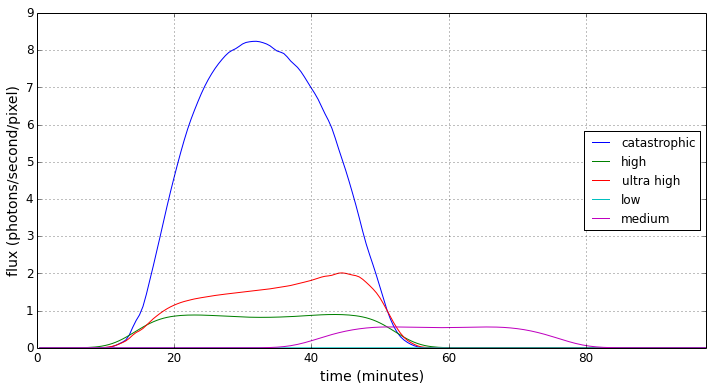
\includegraphics[width=0.8\textwidth]{stray_light.png}\\
    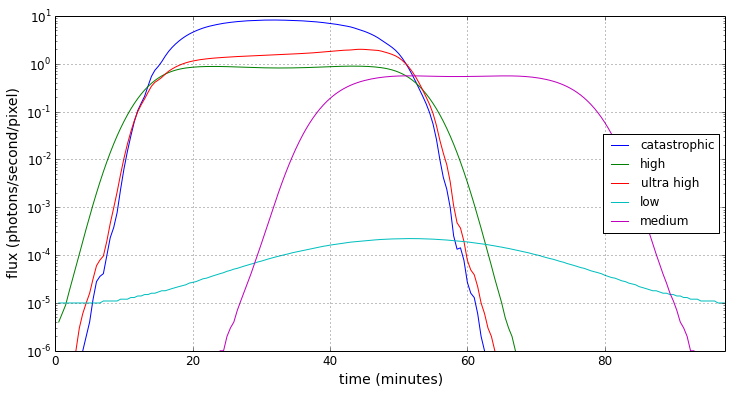
\includegraphics[width=0.8\textwidth]{stray_light_log.png}
    \caption{Stray light intensity as a function of the orbit for a 6am RAAN sun synchronous orbit with altitude of 640km, for five scenarios corresponding to start dates and pointing directions as indicated in Table~\ref{tab:strayLightScenarios}. The same information is shown on a linear (top) and logarithmic (bottom) scale.}
    \label{fig:strayLight}
  \end{center}
\end{figure}

\htmlanchor{strayLightUploadFile}
As an alternative to selecting a pre-existing stray light time series as described above, the user also has the option to upload a file to define the stray light time series. In this case, the time series must be provided as a plain ascii file containing two columns, as defined in Table~\ref{tab:strayLightUploadFormat}. See \href{https://github.com/davefutyan/CHEOPSim/resources/sl_timeseries_6am_SSO650km_medium.dat}{here} for an example.

\begin{table}[hb]
  \begin{center}
  \caption{Columns to be provided in the ascii file for the case of a stray light time series being uploaded by the user. The time series must be provided as a plain ascii file containing the columns indicated (any additional columns will be ignored), separated by whitespace or tab. Rows for which the first character is \# are ignored. It is required that the value of the time in the last row is either longer than the total length of the simulation (including a gap of 30s plus the full frame exposure duration at the start of the visit), or is equal to the default orbit period of 98.5 minutes, in which case the content will be repeated with this periodicity.}
  \begin{tabular}{| l | c | c |}
    \hline
Column & Unit & Format \\
    \hline
Time since start of visit & minutes & float \\
Flux & photons s$^{-1}$pixel$^{-1}$ & float \\
    \hline
  \end{tabular}
  \label{tab:strayLightUploadFormat}
\end{center}
\end{table}

For each time step in the simulation, the stray light flux is added to the image uniformly across the exposed part of the CCD, according to the position within the orbit, and according to the selected scenario.

\htmlanchor{strayLightFromVisitConstraints}
If an MPS\_PRE\_Visits file with an MPS\_PRE\_VisitConstraints extension has been uploaded as described in Section~\ref{sec:time}, then the stray light is read from the MPS\_PRE\_VisitConstraints file by default, although this can be overridden with file upload or pre-existing stray light time series as described above. It is important to read the stray light from MPS\_PRE\_VisitConstraints rather than using one of the pre-existing time series if it is important that the stray light flux is correlated to the orbit position: in the case of the pre-existing time series, the stray light is independent of the orbit model (See the ``important note'' in Section~\ref{sec:OrbitSimulator}).

The stray light filename, as defined in Table~\ref{tab:strayLightScenarios} is the only input parameter for the module (Table~\ref{tab:strayLight}).

\begin{table}[hbtp]
  \caption{Input parameters for the stray light model}

  \htmlanchor{strayLightThreshold}
  \begin{tabular}{| l | p{13cm} |}
    \hline 
    {\bf Parameter} & Stray light threshold for writing out images\\
    {\bf Unit} & photons/s/pixel\\
    {\bf Type / Format} & double\\
    {\bf Default value} & 1.E9\\
    {\bf Comments} & This parameter only applies if no MPS\_PRE\_Visits file has been provided in the Visit tab. Otherwise the threshold is read from that file.\\
    \hline
  \end{tabular}
  \bigskip

  \htmlanchor{strayLightFilename}
  \begin{tabular}{| l | p{13cm} |}
    \hline 
    {\bf Parameter} & Stray light filename\\
    {\bf Unit} & \\
    {\bf Type / Format} & string\\
    {\bf Default value} & sl\_timeseries\_6am\_SSO650km\_medium.dat\\
    {\bf Comments} & See Table~\ref{tab:strayLightScenarios} for available options\\
    \hline
  \end{tabular}
  \bigskip

  \label{tab:strayLight}
\end{table}

\clearpage
\section{Satellite Simulator}
\label{sec:Satellite}

The Satellite Simulator models quantities which vary as a function of the spacecraft orbit, including jitter, FOV rotation, temperature, stray light and particle flux. Each of Sections~\ref{sec:JitterProducer} to \ref{sec:OrbitSimulator} corresponds to a CHEOPSim software module with the indicated name.

\htmlanchor{JitterProducer}
\subsection{Jitter Model:  {\it JitterProducer}}
\label{sec:JitterProducer}

The AOCS jitter time series used by the simulation can be selected from the options specified in Table~\ref{tab:jitter}.
\ifpdf
Further details for each option are provided in Table~\ref{tab:jitter2}.
\fi
If the simulation exceeds the time series duration indicated in
\ifpdf
Table~\ref{tab:jitter2},
\else
Table~\ref{tab:jitter},
\fi
the series is repeated.

Tables~\ref{tab:jitterPlots1} to \ref{tab:jitterPlots5} show, for each time series, a 2-dimensional scatter plot of pitch vs yaw for the entire time series, together with 1-dimensional plots of pitch as a function of time and of yaw as a function of time for the first 10 hours of the time series.

\ifpdf
Table~\ref{tab:jitter2}
\else
Table~\ref{tab:jitter}
\fi
contains a column to indicate whether or not the payload is always in the loop. Cases in which the payload is not always in the loop have interruptions due to SAA and Earth occultations included in the time series. This results in a drift of the jitter while the star trackers are not able to apply corrections, followed by a rapid return to smaller jitter offsets when the star trackers are active again.

Information concerning whether or not the payload is in the loop for a given simulated image is stored in two flags ``VALID\_AOCS'' and ``VALID\_SCIENCE'', which are columns of the \href{https://htmlpreview.github.io/?https://github.com/davefutyan/common_sw/blob/master/doc/fits_data_model/REF_APP_Jitter.html}{REF\_APP\_Jitter} data structure, and of the truth metadata data structures \href{https://htmlpreview.github.io/?https://github.com/davefutyan/common_sw/blob/master/doc/fits_data_model/SIM_TRU_SubArray.html}{SIM\_TRU\_SubArray} and \href{https://htmlpreview.github.io/?https://github.com/davefutyan/common_sw/blob/master/doc/fits_data_model/SIM_TRU_FullArray.html}{SIM\_TRU\_FullArray} (see Section~\ref{sec:truth}). The content of these flags depends on the time series:
\subparagraph{48hrAOCSTimeseries2016\_simu*\_1s.fits}:
\begin{itemize}
\item ``VALID\_AOCS'': FALSE if either the Payload Stellar Estimator (AOCS algorithm for using the payload measurements in the loop) is disabled, or if the instrument centroid is invalid, as is the case during Earth occultation. Otherwise the value is TRUE.
\item ``VALID\_SCIENCE'': Corresponds to the instrument validity flag: FALSE if the instrument centroid is invalid, as is the case during Earth occultation, otherwise TRUE.
\end{itemize}
\subparagraph{All other AOCS time series}:
\begin{itemize}
\item ``VALID\_AOCS'': FALSE if the time corresponds to interruption due to Earth occultation or SAA, otherwise TRUE.
\item ``VALID\_SCIENCE'': TRUE if the pointing direction in the jitter model is at least 35\textdegree above the Earth's atmosphere. It is otherwise set to FALSE, since in this case stray light corrupts the payload measurements for the science mission.
\end{itemize}
%The information contained in these two flags is propagated to the ``STATUS'' keyword of the light curve from photometric extraction (Section~\ref{sec:DataReduction}), whose value maps to the values of the ``VALID\_AOCS'' and ``VALID\_SCIENCE'' flags as shown in Table~\ref{tab:statusFlag}.

{\bf IMPORTANT NOTE:} The ``VALID\_AOCS'' and ``VALID\_SCIENCE'' flags affect only the truth information and do not affect whether or not images are omitted from the output image cube. Images are omitted based on the Earth occultation flag, either read from the MPS\_PRE\_VisitConstraints extension of an input MPS\_PRE\_Visits file, or calculated based on the orbit file and pointing direction, the SAA flag, or the stray light flag (see Section~\ref{sec:omitImages}). These flags is in general independent of the jitter time series, unless a jitter time series has been uploaded which has been generated in such a way as to be in sync with the orbit file.

\htmlanchor{jitterUploadFile}
As an alternative to selecting a pre-existing jitter time series as described above, the user also has the option to upload a jitter time series. In this case, the time series must be provided with 1 second cadence as a plain ascii file containing six columns, and not more than $3600\times48=172800$ rows, as defined in Table~\ref{tab:jitterUploadFormat}.

% \begin{table}[hb]
%   \begin{center}
%   \caption{Definition of values for the ``STATUS'' flag in the extracted light curve}
%   \begin{tabular}{| c | c | c |}
%     \hline
% VALID\_AOCS & VALID\_SCIENCE & STATUS \\
%     \hline
% FALSE&FALSE&0\\
% TRUE&TRUE&1\\
% TRUE&FALSE&2\\
% FALSE&TRUE&3\\
%     \hline
%   \end{tabular}
%   \label{tab:statusFlag}
% \end{center}
% \end{table}

\begin{table}[hbtp]
  \begin{center}
  \caption{Columns to be provided in the ascii file for the case of a jitter time series being uploaded by the user. The time series must be provided as a plain ascii file containing the columns indicated, separated by whitespace or tab. Rows for which the first character is \# are ignored. The cadence must be 1 second and the total number of rows must not exceed $3600\times48=172800$ (i.e. max 48 hour time series).}
  \begin{tabular}{| l | c | c | p{8cm} |}
    \hline
Column & Unit & Format & Notes\\
    \hline
Time & seconds & float & Number of seconds since the start of the time series. Note that the first $N$ seconds can optionally be skipped, where $N$ is a input parameter (see Table~\ref{tab:jitterParameters}).\\
VALID\_AOCS & & boolean (0 or 1) & See main text above for definition\\
VALID\_SCIENCE & & boolean (0 or 1) & See main text above for definition\\
X APE & arcseconds & float & Absolute pointing error around roll axis, aligned to the pointing direction\\
Y APE & arcseconds & float & Absolute pointing error around pitch axis, corresponding to deviations in RA for roll angle = 0\\
Z APE & arcseconds & float & Absolute pointing error around yaw axis, corresponding to deviations in declination for roll angle = 0\\
    \hline
  \end{tabular}
  \label{tab:jitterUploadFormat}
\end{center}
\end{table}

Input parameters to the module are shown in Table~\ref{tab:jitterParameters}. Unless the file upload option is chosen, the name of the jitter file is required as an input parameter, selected via a drop down menu in the web interface.  A second input parameter is a scale factor which can be used to increase the RMS of the jitter by a user specified amount, relative to the the selected jitter file. The RMS for each time series ($\sqrt{rms(pitch)^2+rms(yaw)^2}$) is indicated in Table~\ref{tab:jitter}. If the jitter file is uploaded by the user, an additional parameter can be used to instruct the simulation to omit the first $N$ seconds of the uploaded time series.

The module outputs vectors storing the roll, pitch and yaw Absolute Pointing Errors (APEs) with 1 second time resolution. If {\it OrbitSimulator} is run, then all three APE components are used to calculate the perturbed pointing direction and roll angle at 1 second intervals, as described in Section~\ref{sec:OrbitSimulator}, with these quantities used as input to the projection of the star field onto the CCD plane in {\it FocalPlaneGenerator}. If {\it OrbitSimulator} is not run, then the pointing error about the roll axis is not used, and the pointing errors about the pitch and yaw axes (Y APE and Z APE, respectively) are projected onto the CCD plane in {\it FocalPlaneGenerator} as offsets aligned to the horizontal and vertical directions, respectively, using the plate scale of 1.002 arcsecond per pixel.

\begin{table}[hbtp]
  \caption{Input parameters for the jitter model}

  \htmlanchor{jitterFilename}
  \begin{tabular}{| l | p{13cm} |}
    \hline 
    {\bf Parameter} & Jitter file name\\
    {\bf Unit} & \\
    {\bf Type / Format} & \href{https://htmlpreview.github.io/?https://github.com/davefutyan/common_sw/blob/master/doc/fits_data_model/REF_APP_Jitter.html}{REF\_APP\_Jitter} \\
    {\bf Default value} & \href{https://github.com/davefutyan/CHEOPSim/releases/tag/v1.0}{48hrAOCSTimeseries2016\_simu2\_1s.fits}\\
    {\bf Comments} & \\
    \hline
  \end{tabular}
  \bigskip

  \htmlanchor{jitterScale}
  \begin{tabular}{| l | p{13cm} |}
    \hline 
    {\bf Parameter} & Jitter scale factor\\
    {\bf Unit} & \\
    {\bf Type / Format} & double\\
    {\bf Default value} & 1.0\\
    {\bf Comments} & Scale factor applied to jitter RMS. RMS values for each time series are indicated in Table~\ref{tab:jitter}.\\
    \hline
  \end{tabular}
  \bigskip

  \htmlanchor{jitterFileOffset}
  \begin{tabular}{| l | p{13cm} |}
    \hline 
    {\bf Parameter} & Time offset for uploaded jitter file\\
    {\bf Unit} & seconds\\
    {\bf Type / Format} & double\\
    {\bf Default value} & 0.0\\
    {\bf Comments} & Number of seconds to omit from the start of the uploaded jitter file\\
    \hline
  \end{tabular}
  \bigskip

  \label{tab:jitterParameters}
\end{table}

\clearpage

\ifpdf

\begin{table}[hb]
  \caption{AOCS jitter time series options. The quoted RMS values are ($\sqrt{rms(pitch)^2+rms(yaw)^2}$).}

  \begin{footnotesize}
    \begin{tabular}{| l | c | c | c |}
      \hline
      filename & provider & date provided & R.M.S. \\
      & & & (arcseconds) \\
      \hline
      48hrAOCSTimeseries2016\_simu1\_1s.fits & ADS-CASA & October 2016 & 12.30 \\
      48hrAOCSTimeseries2016\_simu2\_1s.fits & ADS-CASA & October 2016 & 2.24 \\
      48hrAOCSTimeseries2016\_simu3\_1s.fits & ADS-CASA & October 2016 & 5.50 \\
      48hrAOCSTimeseries2016\_simu4\_1s.fits & ADS-CASA & October 2016 & 9.96 \\
      48hrAOCSTimeseries2016\_simu5\_1s.fits & ADS-CASA & October 2016 & 10.52 \\
      48hrAOCSTimeseries2016\_simu6\_1s.fits & ADS-CASA & October 2016 & 12.15 \\
      48hrAOCSTimeseries2016\_simu7\_1s.fits & ADS-CASA & October 2016 & 12.11 \\
      48hrAOCSTimeseries2016\_simu8\_1s.fits & ADS-CASA & October 2016 & 3.03 \\
      48hrAOCSTimeseries2016\_simu9\_1s.fits & ADS-CASA & October 2016 & 5.33 \\
      Case2\_4RW\_1s-May2015-CASA\_notBlinded.fits & ECE-CASA & May 2015 & 1.32 \\
      Case2\_4RW\_1s-Jul2015-CASA\_blinded\_EarthSAA.fits & ECE-CASA & July 2015 & 8.26 \\
      jitter\_ADS-CASA\_4RW\_2ST\_notBlinded\_centroid60s.fits & ADS-CASA & September 2016 & 2.24 \\
      Case2\_4RW\_1s-9Dec2014-CASA.fits & ECE-CASA & December 2014 & 2.82 \\
      Case1\_4RW\_1s-9Dec2014-CASA.fits & ECE-CASA & December 2014 & 1.69 \\
      ESAtimeSeries\_Case2\_4RW\_2OH.fits & ESA & August 2014 & 3.40 \\
      Case2\_4RW\_1s.fits & ECE-CASA & February 2014 & 3.11 \\
      Case2\_3RW\_1s.fits & ECE-CASA & February 2014 & 3.12 \\
      Case1\_4RW\_1s.fits & ECE-CASA & February 2014 & 1.73 \\
      Case1\_3RW\_1s.fits & ECE-CASA & February 2014 & 1.73 \\
      Case2\_1STR\_1s.fits & ECE-CASA & February 2014 & 5.92 \\
      Case2\_1hz\_1s.fits & ECE-CASA & February 2014 & 2.61 \\
      \hline
    \end{tabular}

  \end{footnotesize}
  \label{tab:jitter}
\end{table}

\begin{table}[hb]
  \caption{AOCS jitter time series options (continued). The payload in the loop column indicates whether or not interruptions due to SAA and Earth occultations are included.}

  \begin{footnotesize}
    \begin{tabular}{| p{5.5cm} | c | c | c | c  | c | c | c |}
      \hline
      filename & time series & No. of & No. of & payload & payload & Altitude & LoS w.r.t. \\
      & duration & reaction& star & sampling & always & (km) & orbital \\
      & (hours) & wheels & trackers & cadence (s) & in loop & & plane \\
      \hline
      48hrAOCSTimeseries2016\_simu1\_1s.fits & 48 & 4 & 2 & 60 & never & 700 & \\
      48hrAOCSTimeseries2016\_simu2\_1s.fits & 48 & 4 & 2 & 60 & yes & 700 & \\
      48hrAOCSTimeseries2016\_simu3\_1s.fits  & 48 & 3 & 1 & 60 & yes & 700 & \\
      48hrAOCSTimeseries2016\_simu4\_1s.fits  & 48 & 4 & 2 & 60 & no &  700& \\
      48hrAOCSTimeseries2016\_simu5\_1s.fits  & 48 & 3 & 2 & 60 & no & 700 & \\
      48hrAOCSTimeseries2016\_simu6\_1s.fits  & 48 & 4 & 1 & 60 & no & 700 & \\
      48hrAOCSTimeseries2016\_simu7\_1s.fits  & 48 & 3 & 1 & 1 & no & 700 & \\
      48hrAOCSTimeseries2016\_simu8\_1s.fits  & 48 & 4 & 2 & 60 & no & 700 & \\
      48hrAOCSTimeseries2016\_simu9\_1s.fits  & 48 & 4 & 1 & 60 & no & 700 & \\
      Case2\_4RW\_1s-May2015-CASA\_notBlinded.fits & 48 & 4 & 2 & & yes & 800 & \\
      Case2\_4RW\_1s-Jul2015-CASA\_blinded\_EarthSAA.fits & 48 & 4 & 2 & & no & 800 & 15 degrees \\
      jitter\_ADS-CASA\_4RW\_2ST \_notBlinded\_centroid60s.fits & 48 & 4 & 2 & 60 & yes & 700 & \\
      Case2\_4RW\_1s-9Dec2014-CASA.fits & 48 & 4  & 2 & & no & 800 & \\
      Case1\_4RW\_1s-9Dec2014-CASA.fits & 48 & 4  & 2 & & no & 650 & \\
      ESAtimeSeries\_Case2\_4RW\_2OH.fits & 48 & 4 & 2 & & no & & 10 degrees \\
      Case2\_4RW\_1s.fits & 10 & 4 & 2 & 60 & no & & 10 degrees \\
      Case2\_3RW\_1s.fits & 10 & 3 & 2 & 60 & no & & 10 degrees \\
      Case1\_4RW\_1s.fits & 10 & 4 & 2 & 60 & no & & perpendicular \\
      Case1\_3RW\_1s.fits & 10 & 3 & 2 & 60 & no & & perpendicular \\
      Case2\_1STR\_1s.fits & 10 & 4 & 1 & 60 & no & & 10 degrees \\
      Case2\_1hz\_1s.fits & 10 & 4 & 2 & 1 & no & & 10 degrees \\
      \hline
    \end{tabular}

  \end{footnotesize}
  \label{tab:jitter2}
\end{table}

\else

\begin{table}[hb]
  \caption{AOCS jitter time series options. The quoted RMS values are ($\sqrt{rms(pitch)^2+rms(yaw)^2}$). The payload in the loop column indicates whether or not interruptions due to SAA and Earth occultations are included.}

  \begin{tabular}{| l | c | c | c | c  | c | c | c | c | c | c |}
    \hline
    filename & provider & date provided & time series & No. of & No. of & payload & payload & Altitude & LoS w.r.t.  & R.M.S. \\
    & & & duration & reaction& star & sampling & always & (km) & orbital & (arcseconds) \\
    & & & (hours) & wheels & trackers & cadence (s) & in loop & & plane & \\
\hline
    48hrAOCSTimeseries2016\_ simu1\_1s.fits & ADS-CASA & October 2016 & 48 & 4 & 2 & 60 & never & 700 & & 12.30 \\
    48hrAOCSTimeseries2016\_ simu2\_1s.fits & ADS-CASA & October 2016 & 48 & 4 & 2 & 60 & yes & 700 & & 2.24 \\
    48hrAOCSTimeseries2016\_ simu3\_1s.fits & ADS-CASA & October 2016 & 48 & 3 & 1 & 60 & yes & 700 & & 5.50 \\
    48hrAOCSTimeseries2016\_ simu4\_1s.fits & ADS-CASA & October 2016 & 48 & 4 & 2 & 60 & no & 700 & & 9.96 \\
    48hrAOCSTimeseries2016\_ simu5\_1s.fits & ADS-CASA & October 2016 & 48 & 3 & 2 & 60 & no & 700 & & 10.52 \\
    48hrAOCSTimeseries2016\_ simu6\_1s.fits & ADS-CASA & October 2016 & 48 & 4 & 1 & 60 & no & 700 & & 12.15 \\
    48hrAOCSTimeseries2016\_ simu7\_1s.fits & ADS-CASA & October 2016 & 48 & 3 & 1 & 1 & no & 700 & & 12.11 \\
    48hrAOCSTimeseries2016\_ simu8\_1s.fits & ADS-CASA & October 2016 & 48 & 4 & 2 & 60 & no & 700 & & 3.03 \\
    48hrAOCSTimeseries2016\_ simu9\_1s.fits & ADS-CASA & October 2016 & 48 & 4 & 1 & 60 & no & 700 & & 5.33 \\
    Case2\_4RW\_1s-May2015-CASA\_notBlinded.fits & ECE-CASA & May 2015 & 48 & 4 & 2 & & yes & 800 & & 1.32 \\
    Case2\_4RW\_1s-Jul2015-CASA\_blinded\_EarthSAA.fits & ECE-CASA & July 2015 & 48 & 4 & 2 & & no & 800 & 15 degrees & 8.26 \\
     jitter\_ADS-CASA\_4RW\_2ST\_notBlinded\_centroid60s.fits & ADS-CASA & September 2016 & 48 & 4 & 2 & 60 & yes & 700 & & 2.24 \\
    Case2\_4RW\_1s-9Dec2014-CASA.fits & ECE-CASA & December 2014 & 48 & 4  & 2 & & no & 800 & & 2.82 \\
    Case1\_4RW\_1s-9Dec2014-CASA.fits & ECE-CASA & December 2014 & 48 & 4  & 2 & & no & 650 & & 1.69 \\
    ESAtimeSeries\_Case2\_4RW\_2OH.fits & ESA & August 2014 & 48 & 4 & 2 & & no & & 10 degrees & 3.40 \\
    Case2\_4RW\_1s.fits & ECE-CASA & February 2014 & 10 & 4 & 2 & 60 & no & & 10 degrees & 3.11 \\
    Case2\_3RW\_1s.fits & ECE-CASA & February 2014 & 10 & 3 & 2 & 60 & no & & 10 degrees & 3.12 \\
    Case1\_4RW\_1s.fits & ECE-CASA & February 2014 & 10 & 4 & 2 & 60 & no & & perpendicular & 1.73 \\
    Case1\_3RW\_1s.fits & ECE-CASA & February 2014 & 10 & 3 & 2 & 60 & no & & perpendicular & 1.73 \\
    Case2\_1STR\_1s.fits & ECE-CASA & February 2014 & 10 & 4 & 1 & 60 & no & & 10 degrees & 5.92 \\
    Case2\_1hz\_1s.fits & ECE-CASA & February 2014 & 10 & 4 & 2 & 1 & no & & 10 degrees & 2.61 \\
    \hline
  \end{tabular}

  \label{tab:jitter}
\end{table}

\fi

\begin{table}[hb]
  \caption{AOCS jitter time series plots}
  \ifpdf
  \begin{tabular}{| m{4.6cm} c c |}
    \else 
    \begin{tabular}{| l c c |}
    \fi
    \hline
    48hrAOCSTimeseries2016\_ simu1\_1s.fits& \href{48hrAOCSTimeseries2016_simu1_2D.png}{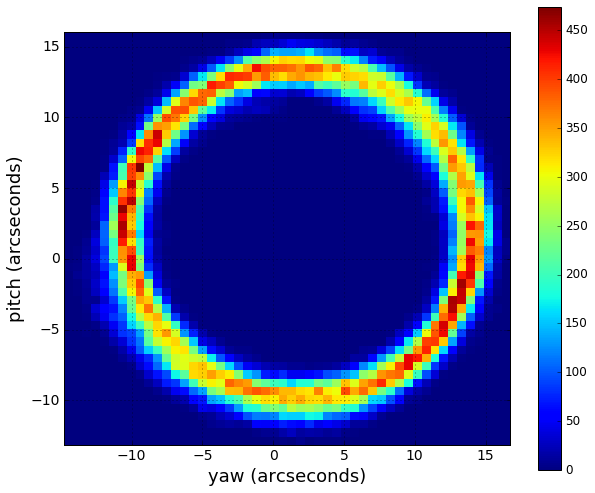
\includegraphics[valign=m,width=0.27\textwidth]{48hrAOCSTimeseries2016_simu1_2D.png}} & \href{48hrAOCSTimeseries2016_simu1_1D.png}{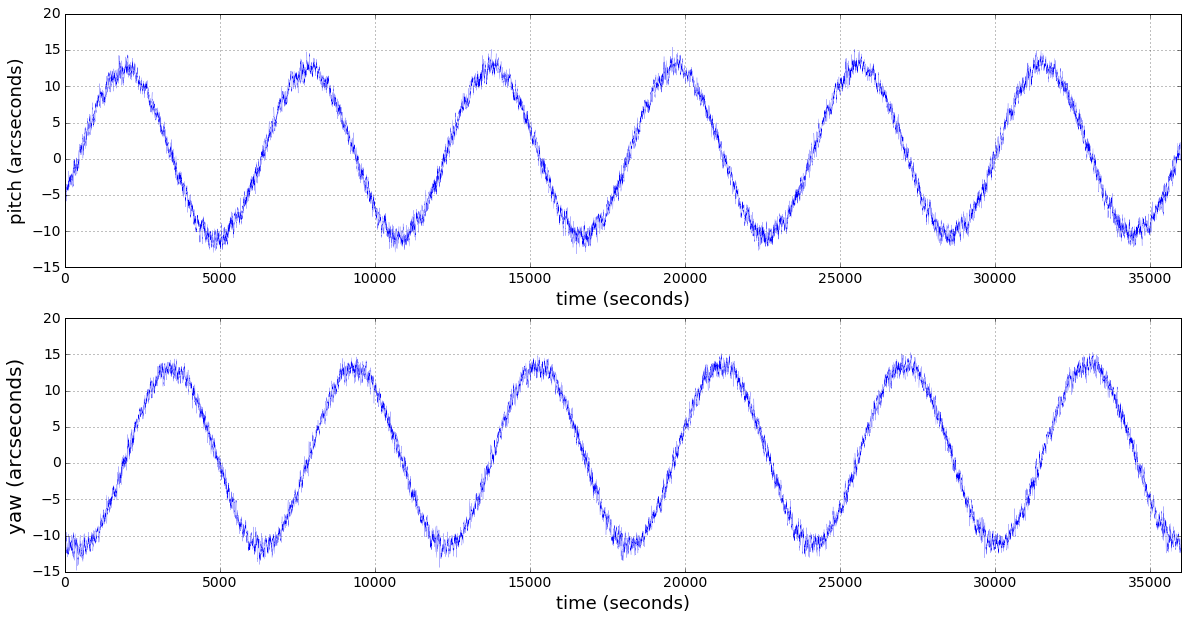
\includegraphics[valign=m,width=0.45\textwidth]{48hrAOCSTimeseries2016_simu1_1D.png}}\\
    \hline
    48hrAOCSTimeseries2016\_ simu2\_1s.fits& \href{48hrAOCSTimeseries2016_simu2_2D.png}{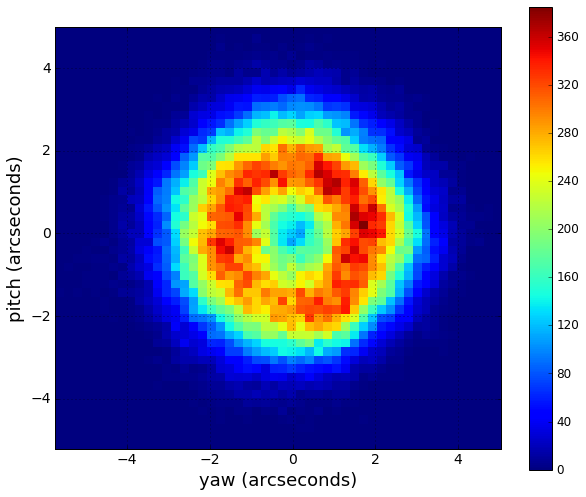
\includegraphics[valign=m,width=0.27\textwidth]{48hrAOCSTimeseries2016_simu2_2D.png}} & \href{48hrAOCSTimeseries2016_simu2_1D.png}{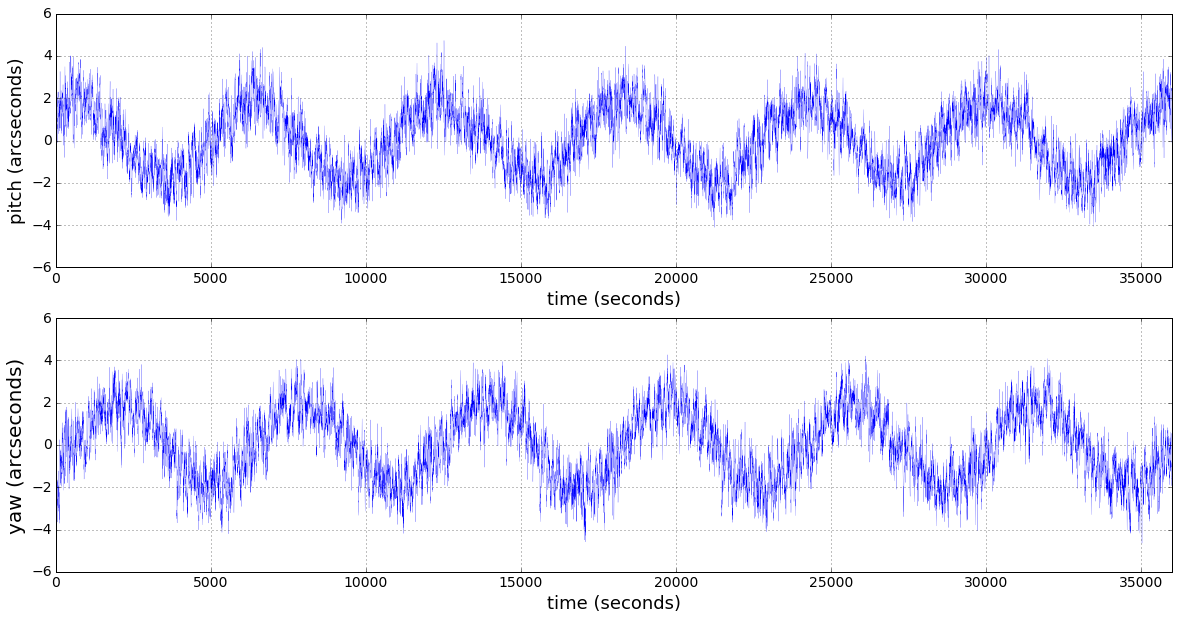
\includegraphics[valign=m,width=0.45\textwidth]{48hrAOCSTimeseries2016_simu2_1D.png}}\\
    \hline
    48hrAOCSTimeseries2016\_ simu3\_1s.fits& \href{48hrAOCSTimeseries2016_simu3_2D.png}{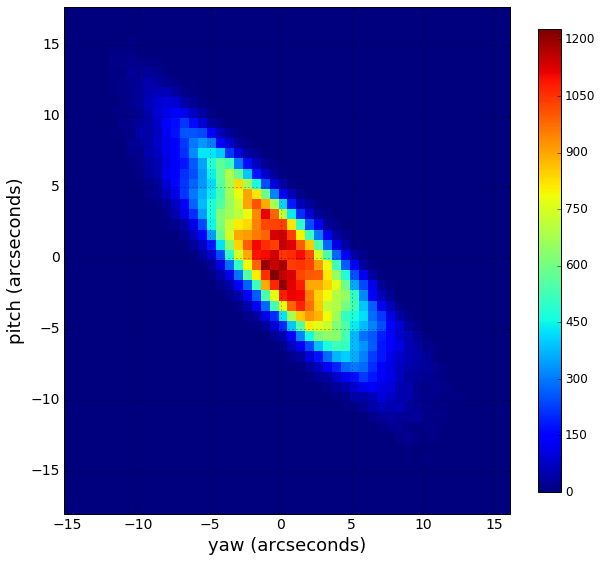
\includegraphics[valign=m,width=0.27\textwidth]{48hrAOCSTimeseries2016_simu3_2D.png}} & \href{48hrAOCSTimeseries2016_simu3_1D.png}{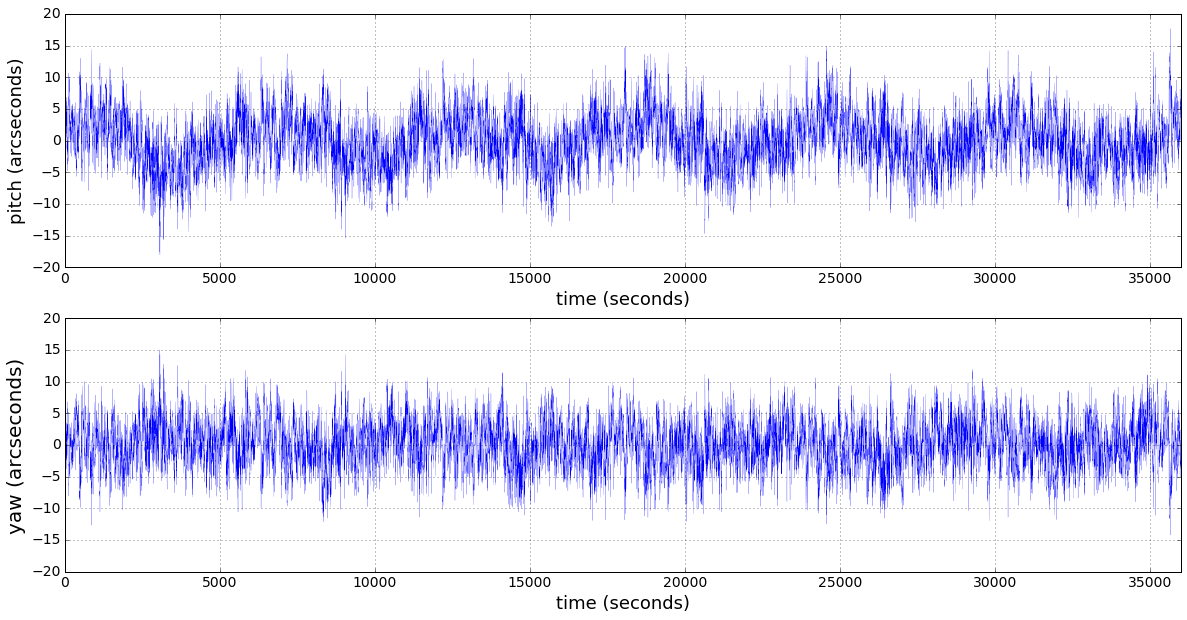
\includegraphics[valign=m,width=0.45\textwidth]{48hrAOCSTimeseries2016_simu3_1D.png}}\\
    \hline
  \end{tabular}
  \label{tab:jitterPlots1}
\end{table}

\begin{table}[hb]
  \caption{AOCS jitter time series plots (continued)}
  \ifpdf
  \begin{tabular}{| m{4.6cm} c c |}
    \else 
    \begin{tabular}{| l c c |}
    \fi
    \hline
    48hrAOCSTimeseries2016\_ simu4\_1s.fits& \href{48hrAOCSTimeseries2016_simu4_2D.png}{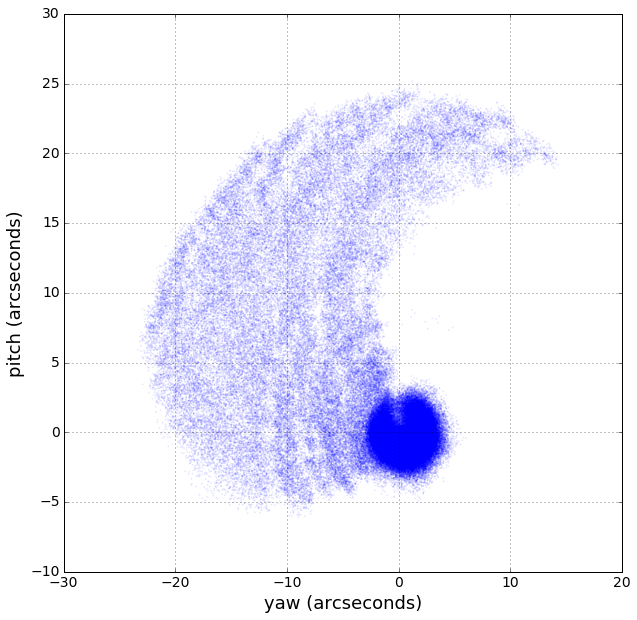
\includegraphics[valign=m,width=0.225\textwidth]{48hrAOCSTimeseries2016_simu4_2D.png}} & \href{48hrAOCSTimeseries2016_simu4_1D.png}{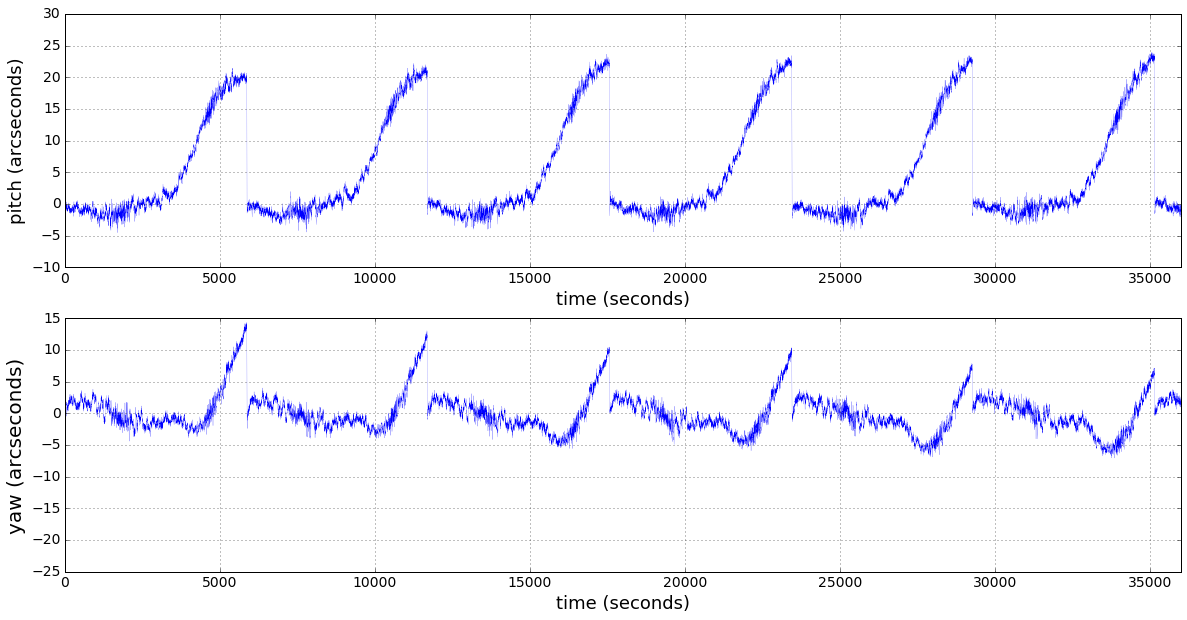
\includegraphics[valign=m,width=0.36\textwidth]{48hrAOCSTimeseries2016_simu4_1D.png}}\\
    \hline
    48hrAOCSTimeseries2016\_ simu5\_1s.fits& \href{48hrAOCSTimeseries2016_simu5_2D.png}{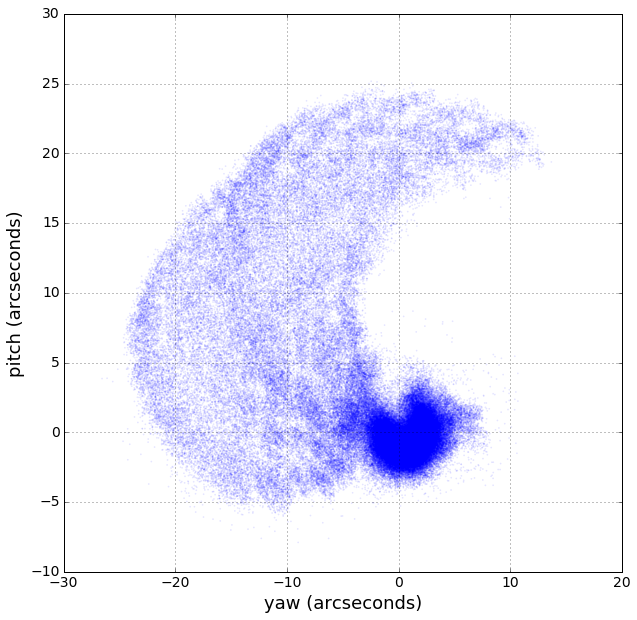
\includegraphics[valign=m,width=0.225\textwidth]{48hrAOCSTimeseries2016_simu5_2D.png}} & \href{48hrAOCSTimeseries2016_simu5_1D.png}{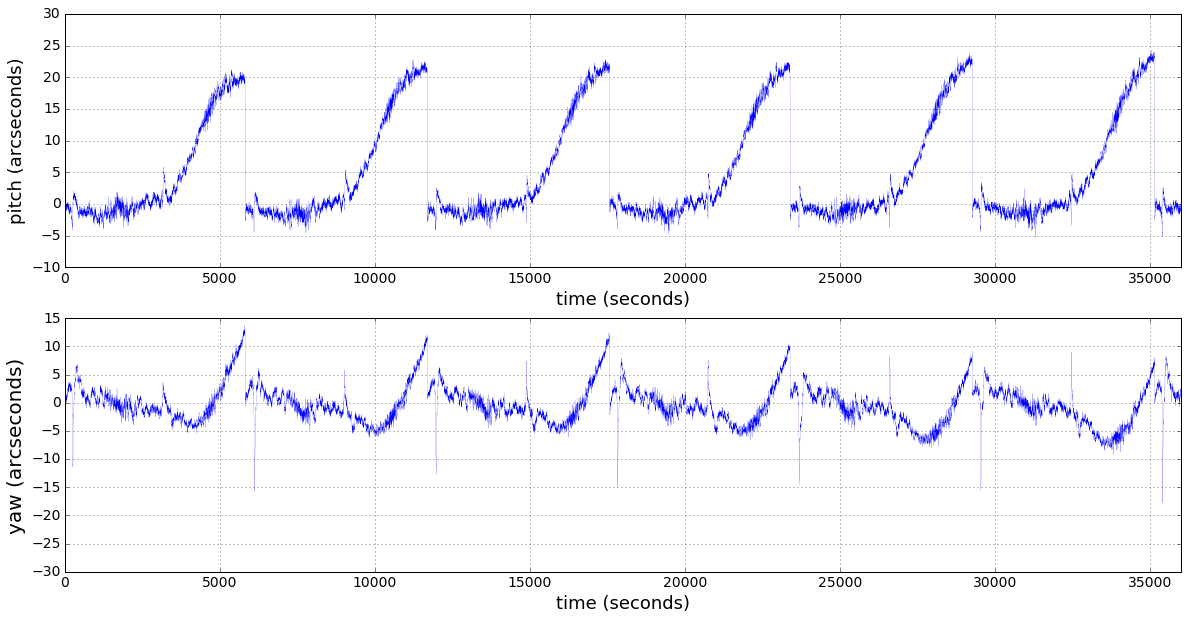
\includegraphics[valign=m,width=0.36\textwidth]{48hrAOCSTimeseries2016_simu5_1D.png}}\\
    \hline
    48hrAOCSTimeseries2016\_ simu6\_1s.fits& \href{48hrAOCSTimeseries2016_simu6_2D.png}{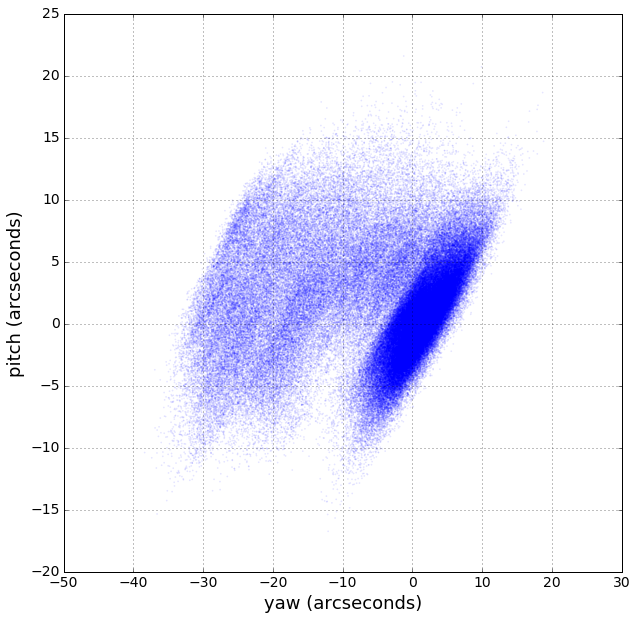
\includegraphics[valign=m,width=0.225\textwidth]{48hrAOCSTimeseries2016_simu6_2D.png}} & \href{48hrAOCSTimeseries2016_simu6_1D.png}{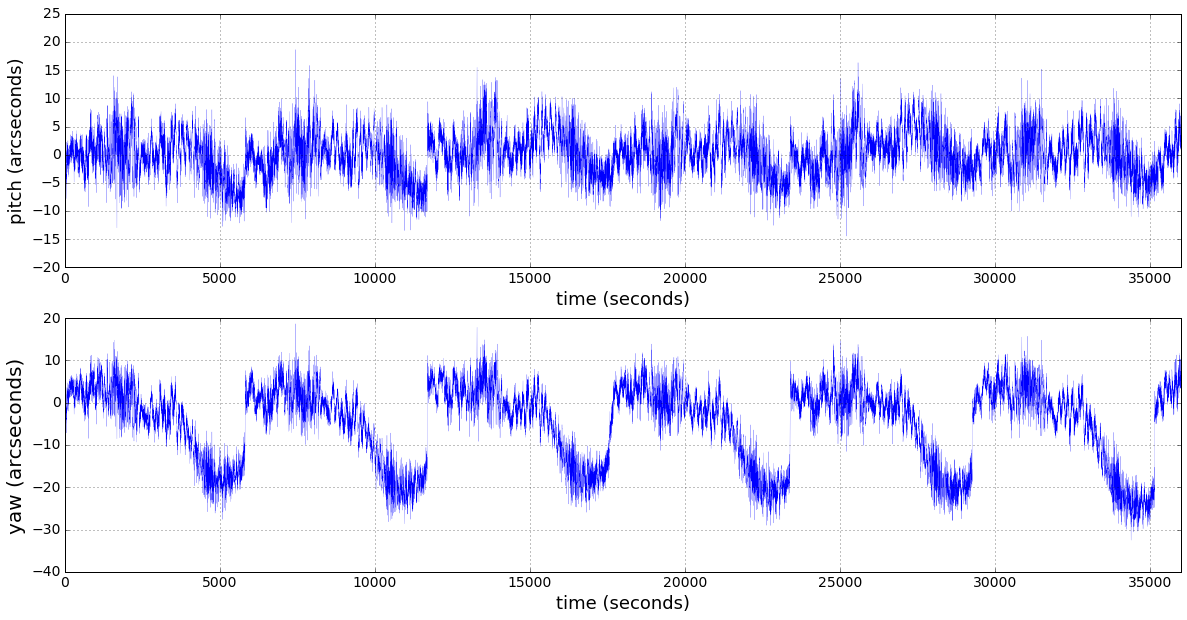
\includegraphics[valign=m,width=0.36\textwidth]{48hrAOCSTimeseries2016_simu6_1D.png}}\\
    \hline
    48hrAOCSTimeseries2016\_ simu7\_1s.fits& \href{48hrAOCSTimeseries2016_simu7_2D.png}{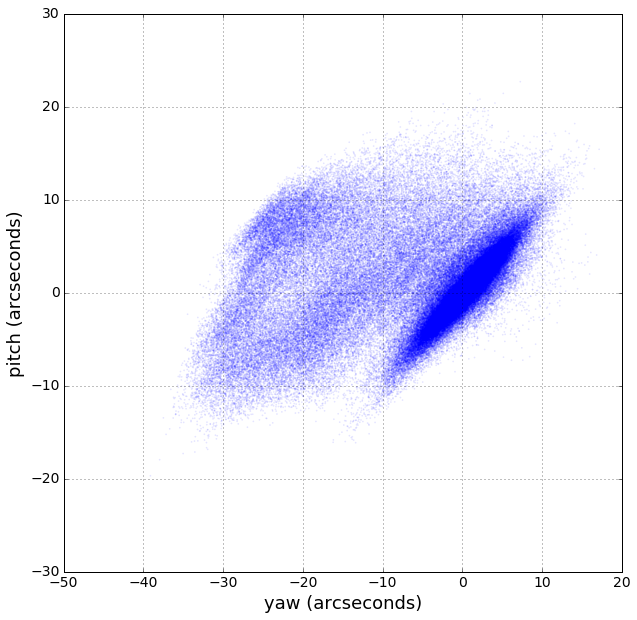
\includegraphics[valign=m,width=0.225\textwidth]{48hrAOCSTimeseries2016_simu7_2D.png}} & \href{48hrAOCSTimeseries2016_simu7_1D.png}{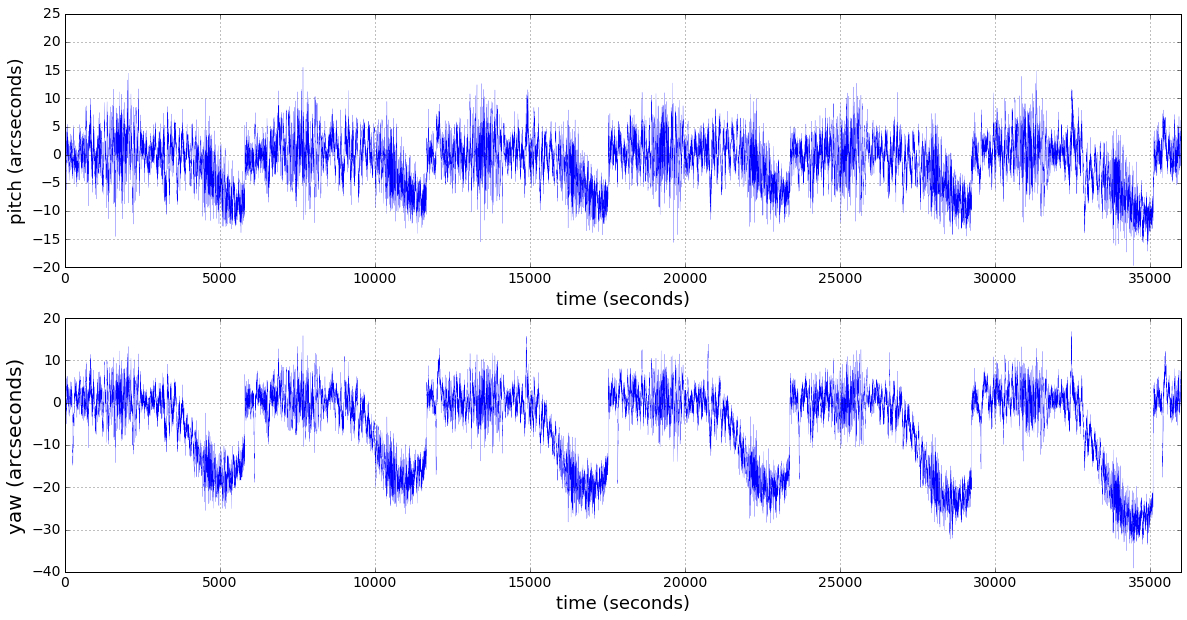
\includegraphics[valign=m,width=0.36\textwidth]{48hrAOCSTimeseries2016_simu7_1D.png}}\\
    \hline
    48hrAOCSTimeseries2016\_ simu8\_1s.fits& \href{48hrAOCSTimeseries2016_simu8_2D.png}{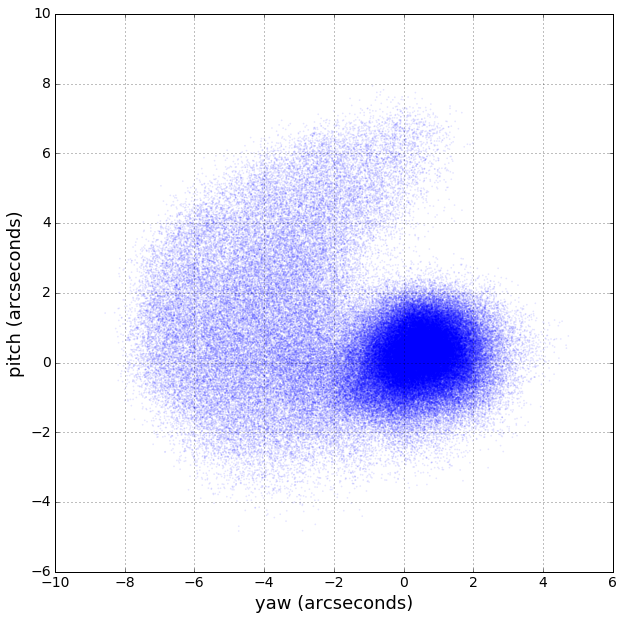
\includegraphics[valign=m,width=0.225\textwidth]{48hrAOCSTimeseries2016_simu8_2D.png}} & \href{48hrAOCSTimeseries2016_simu8_1D.png}{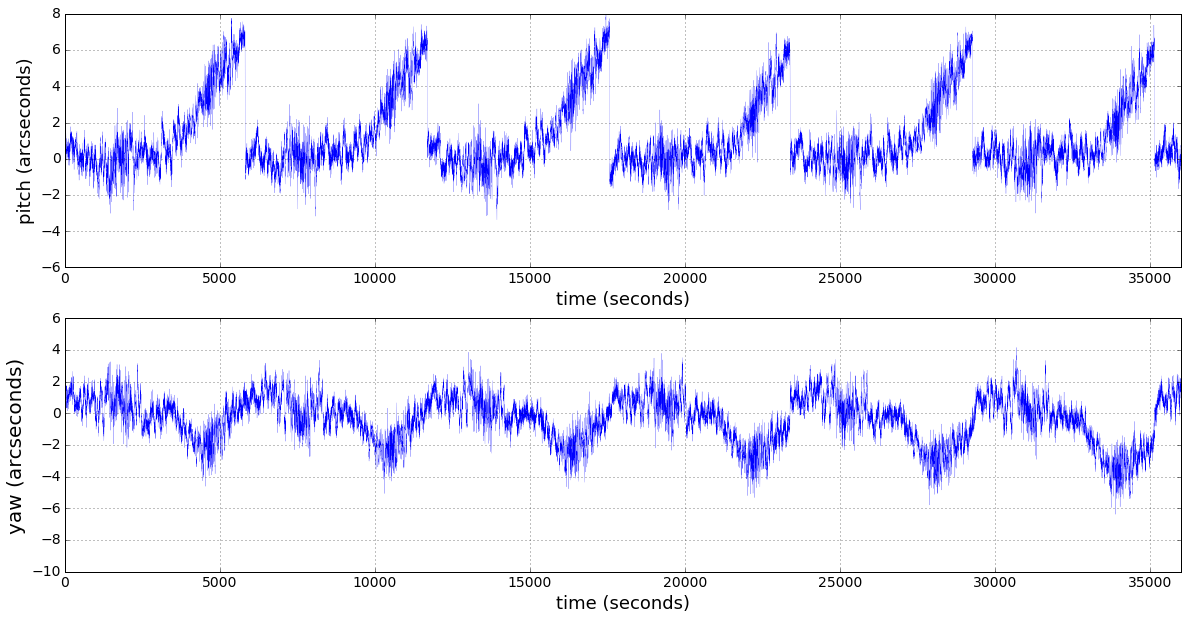
\includegraphics[valign=m,width=0.36\textwidth]{48hrAOCSTimeseries2016_simu8_1D.png}}\\
    \hline
    48hrAOCSTimeseries2016\_ simu9\_1s.fits& \href{48hrAOCSTimeseries2016_simu9_2D.png}{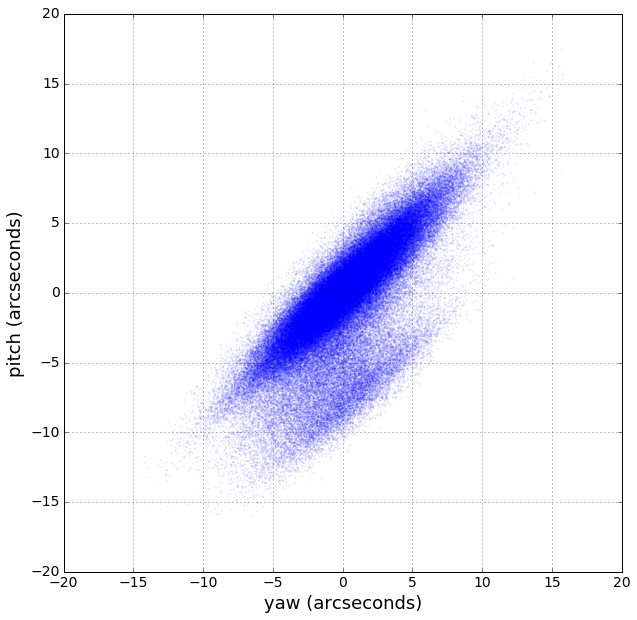
\includegraphics[valign=m,width=0.225\textwidth]{48hrAOCSTimeseries2016_simu9_2D.png}} & \href{48hrAOCSTimeseries2016_simu9_1D.png}{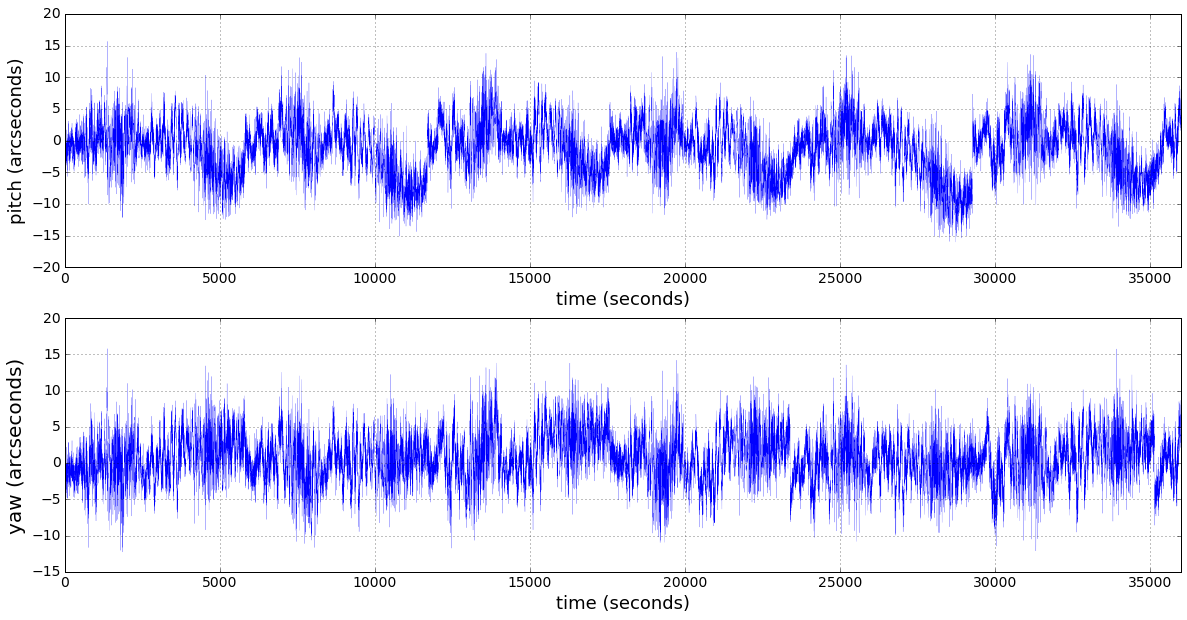
\includegraphics[valign=m,width=0.36\textwidth]{48hrAOCSTimeseries2016_simu9_1D.png}}\\
    \hline
  \end{tabular}
  \label{tab:jitterPlots2}
\end{table}

\begin{table}[hb]
  \caption{AOCS jitter time series plots (continued)}
  \ifpdf
  \begin{tabular}{| m{3.5cm} c c |}
    \else 
    \begin{tabular}{| l c c |}
    \fi
    \hline
    Case2\_4RW\_1s-May2015-CASA\_notBlinded.fits & \href{Case2_4RW_1s-May2015-CASA_notBlinded_2D.png}{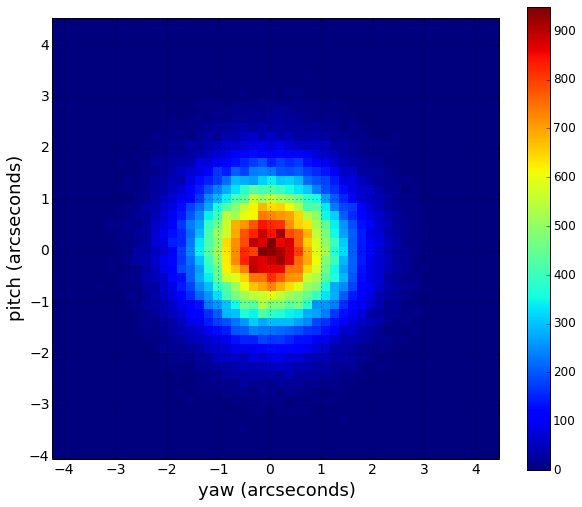
\includegraphics[valign=m,width=0.3\textwidth]{Case2_4RW_1s-May2015-CASA_notBlinded_2D.png}} & \href{Case2_4RW_1s-May2015-CASA_notBlinded_1D.png}{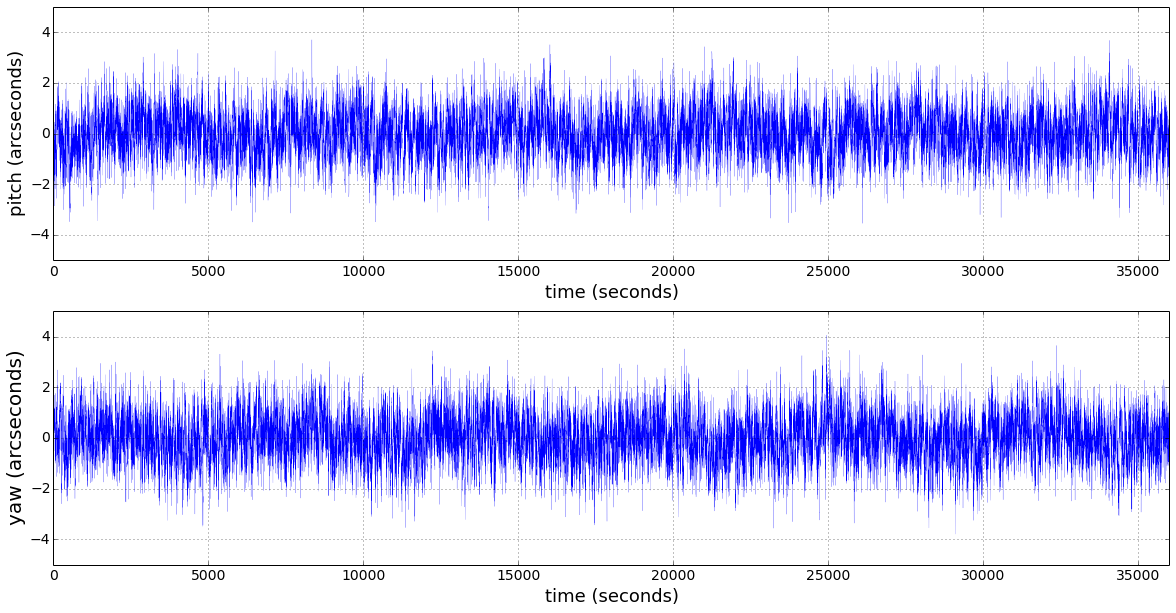
\includegraphics[valign=m,width=0.5\textwidth]{Case2_4RW_1s-May2015-CASA_notBlinded_1D.png}}\\
    \hline
    Case2\_4RW\_1s-Jul2015-CASA\_ blinded\_EarthSAA.fits & \href{Case2_4RW_1s-Jul2015-CASA_blinded_EarthSAA_2D.png}{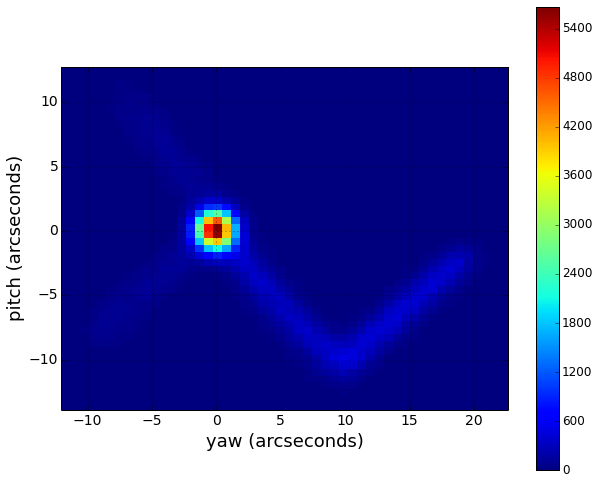
\includegraphics[valign=m,width=0.3\textwidth]{Case2_4RW_1s-Jul2015-CASA_blinded_EarthSAA_2D.png}} & \href{Case2_4RW_1s-Jul2015-CASA_blinded_EarthSAA_1D.png}{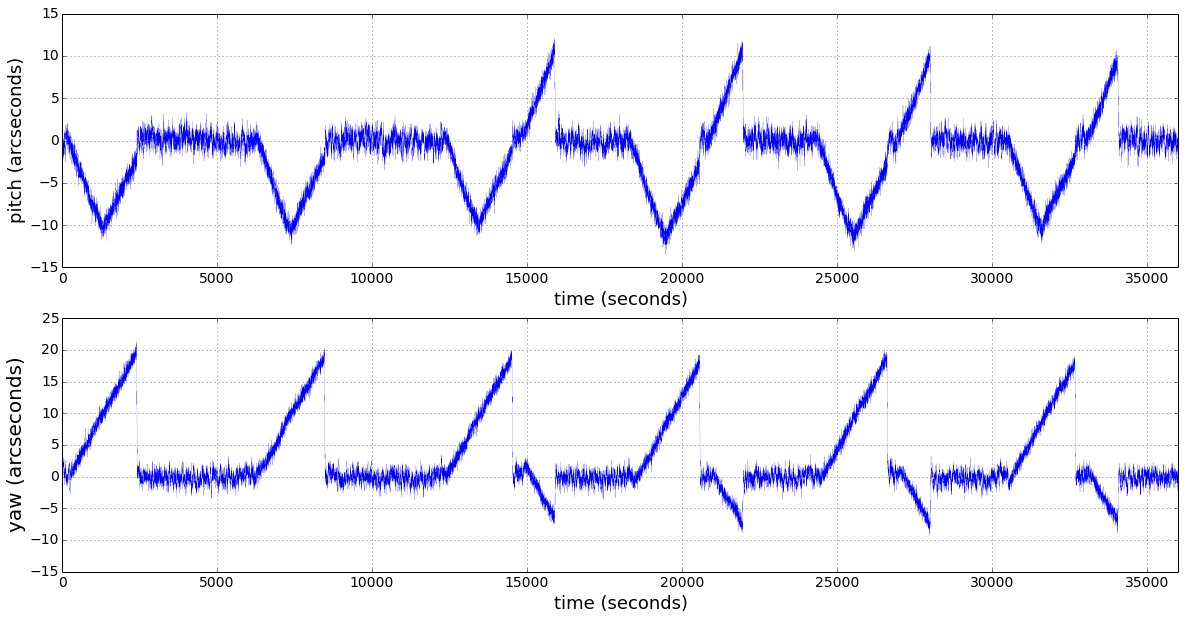
\includegraphics[valign=m,width=0.5\textwidth]{Case2_4RW_1s-Jul2015-CASA_blinded_EarthSAA_1D.png}}\\
    \hline
     jitter\_ADS-CASA\_4RW\_2ST\_\-notBlinded\-\_centroid60s.fits & \href{jitter_ADS-CASA_4RW_2ST_notBlinded_centroid60s_2D.png}{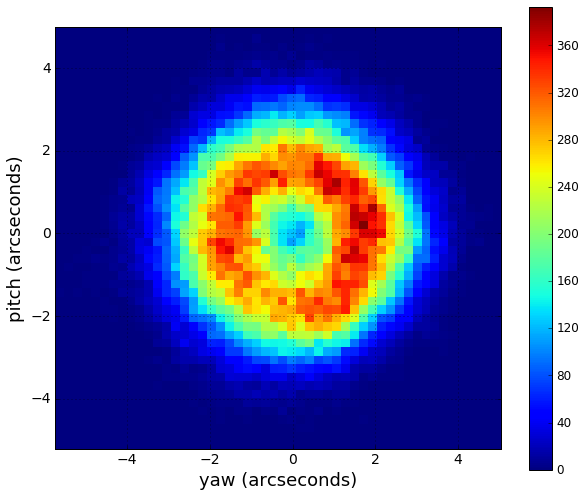
\includegraphics[valign=m,width=0.3\textwidth]{jitter_ADS-CASA_4RW_2ST_notBlinded_centroid60s_2D.png}} & \href{jitter_ADS-CASA_4RW_2ST_notBlinded_centroid60s_1D.png}{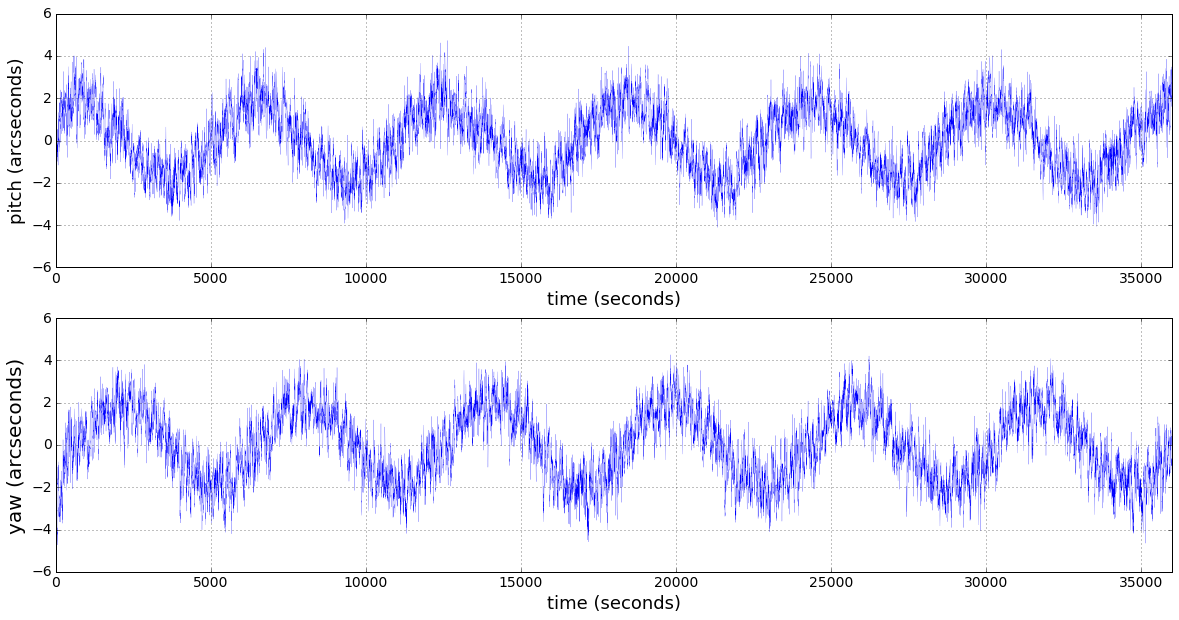
\includegraphics[valign=m,width=0.5\textwidth]{jitter_ADS-CASA_4RW_2ST_notBlinded_centroid60s_1D.png}}\\
    \hline
  \end{tabular}
  \label{tab:jitterPlots3}
\end{table}

\begin{table}[hb]
  \caption{AOCS jitter time series plots (continued)}
  \ifpdf
  \begin{tabular}{| m{3.5cm} c c |}
    \else 
    \begin{tabular}{| l c c |}
    \fi
    \hline
    Case2\_4RW\_1s-9Dec2014-CASA.fits& \href{Case2_4RW_9Dec2014_2D.png}{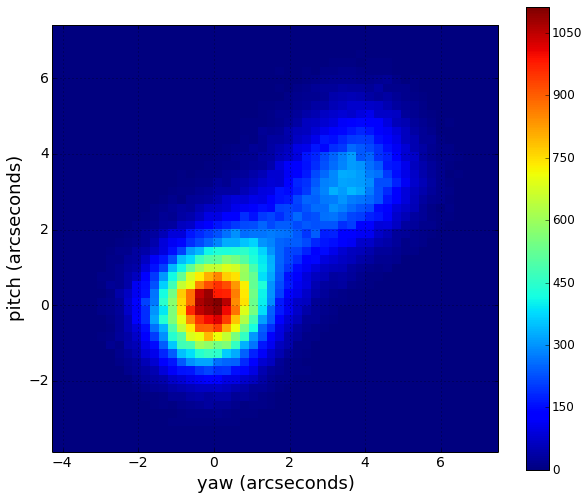
\includegraphics[valign=m,width=0.3\textwidth]{Case2_4RW_9Dec2014_2D.png}} & \href{Case2_4RW_9Dec2014_1D.png}{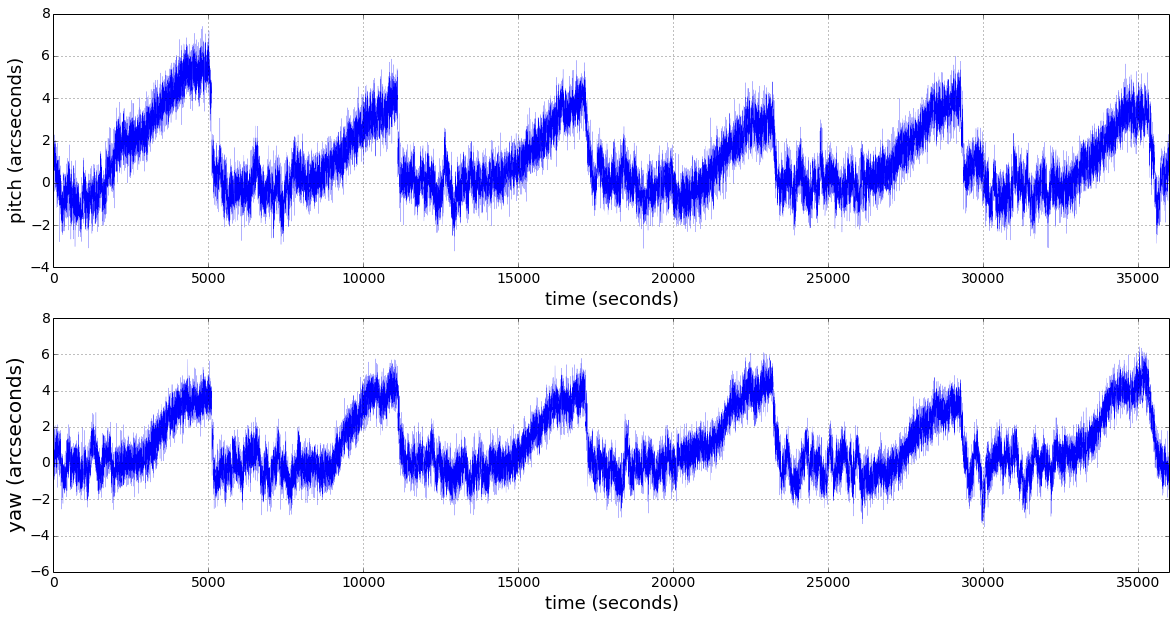
\includegraphics[valign=m,width=0.5\textwidth]{Case2_4RW_9Dec2014_1D.png}}\\
    \hline
    Case1\_4RW\_1s-9Dec2014-CASA.fits & \href{Case1_4RW_9Dec2014_2D.png}{\includegraphics[valign=m,width=0.3\textwidth]{Case1_4RW_9Dec2014_2D.png}} & \href{Case1_4RW_9Dec2014_1D.png}{\includegraphics[valign=m,width=0.5\textwidth]{Case1_4RW_9Dec2014_1D.png}}\\
    \hline
    ESAtimeSeries\_Case2\_ 4RW\_2OH.fits & \href{ESAtimeSeries_Case2_4RW_2OH_2D.png}{\includegraphics[valign=m,width=0.3\textwidth]{ESAtimeSeries_Case2_4RW_2OH_2D.png}} & \href{ESAtimeSeries_Case2_4RW_2OH_1D.png}{\includegraphics[valign=m,width=0.5\textwidth]{ESAtimeSeries_Case2_4RW_2OH_1D.png}}\\
    \hline
  \end{tabular}
  \label{tab:jitterPlots4}
\end{table}

\begin{table}[hb]
  \caption{AOCS jitter time series plots (continued)}
  \begin{tabular}{| l c c |}
    \hline
    Case2\_4RW\_1s.fits & \href{Case2_4RW_2D.png}{\includegraphics[valign=m,width=0.25\textwidth]{Case2_4RW_2D.png}} & \href{Case2_4RW_1D.png}{\includegraphics[valign=m,width=0.4\textwidth]{Case2_4RW_1D.png}}\\
    \hline
    Case2\_3RW\_1s.fits & \href{Case2_3RW_2D.png}{\includegraphics[valign=m,width=0.25\textwidth]{Case2_3RW_2D.png}} & \href{Case2_3RW_1D.png}{\includegraphics[valign=m,width=0.4\textwidth]{Case2_3RW_1D.png}}\\
    \hline
    Case1\_4RW\_1s.fits & \href{Case1_4RW_2D.png}{\includegraphics[valign=m,width=0.25\textwidth]{Case1_4RW_2D.png}} & \href{Case1_4RW_1D.png}{\includegraphics[valign=m,width=0.4\textwidth]{Case1_4RW_1D.png}}\\
    \hline
    Case1\_3RW\_1s.fits & \href{Case1_3RW_2D.png}{\includegraphics[valign=m,width=0.25\textwidth]{Case1_3RW_2D.png}} & \href{Case1_3RW_1D.png}{\includegraphics[valign=m,width=0.4\textwidth]{Case1_3RW_1D.png}}\\
    \hline
    Case2\_1STR\_1s.fits & \href{Case2_1STR_2D.png}{\includegraphics[valign=m,width=0.25\textwidth]{Case2_1STR_2D.png}} & \href{Case2_1STR_1D.png}{\includegraphics[valign=m,width=0.4\textwidth]{Case2_1STR_1D.png}}\\
    \hline
    Case2\_1hz\_1s.fits & \href{Case2_1hz_2D.png}{\includegraphics[valign=m,width=0.25\textwidth]{Case2_1hz_2D.png}} & \href{Case2_1hz_1D.png}{\includegraphics[valign=m,width=0.4\textwidth]{Case2_1hz_1D.png}}\\
    \hline 
  \end{tabular}
  \label{tab:jitterPlots5}
\end{table}

\clearpage
\htmlanchor{OrbitSimulator}
\subsection{Orbit Model:  {\it OrbitSimulator}}
\label{sec:OrbitSimulator}

The role of the {\it OrbitSimulator} module is to simulate the variation of relevant quantities which depend on the position of the satellite within its orbit.

\subsubsection{Orbit Trajectory, Pointing Jitter and Roll Angle}

The default trajectory file is provided by INTA. It specifyies the position of the spacecraft in Earth Centred Inertial frame coordinates (EME2000) for a sun synchronous orbit at an altitude of 700km, for Local Time of Ascending Node (LTAN)  6am, at 1 minute intervals, from 31 Dec 2018 00:00 to 2 Aug 2022 00:00. Alternative trajectory files are provided by ESOC at 1 minute intervals from 1 Jan 2018 00:00 to 31 Dec 20180 23:59, for sun synchronous orbits at altitudes of 650km, 700km and 800km, and, for each of these altitudes, for Local Time of Ascending Node (LTAN) values of 6am and 6pm. The trajectory file is an input parameter for the module (Table~\ref{tab:orbit1} ).

The instantaneous velocity of the spacecraft in the inertial frame at any given time is calculated as the vector difference between the spacecraft positions one minute before and one minute after the current time, divided by the duration separating those positions (two minutes). Positions and velocities at time intervals smaller than one minute are calculated by linear interpolation.

The roll angle at any given time is calculated using as input the pointing direction, the position vector and the velocity vector of the spacecraft in the intertial frame at that time, using an algorithm provided by ESA~\cite{rollAngleAlgo}. The algorithm calculates the rotation matrices to transform between the inertial frame, the Local Vertical / Local Horizontal (LVLH) frame, the orbital frame, and the satellite frame. The roll angle is then extracted from the matrix elements of the rotation matrix from the inertial to the satellite frame, $M_{i2sat}$, as follows (indices starting from 0):

\[roll\ angle = atan2 ( M_{i2sat}[1,2], M_{i2sat}[2,2] )\]

If {\it JitterProducer} has been run, then the Absolute Pointing Errors (APEs) output by that module (at 1 second intervals) are used to calculate the perturbations to the pointing direction and to the roll angle at any given time. The perturbation to the pointing direction is calculated as follows:

\[m_{point} = {M_{i2sat}}^T\ dR\ M_{i2sat}\ m_{nominalPoint}\]

where $m_{nominalPoint}$ and $m_{point}$ are the pointing vectors in cartesian coordinates before and after applying the APEs, and dR is the APE rotation matrix:

\[
dR = \begin{bmatrix} 
1 & -APE_Z & APE_Y \\ 
APE_Z & 1 & -APE_X \\ 
-APE_Y & APE_X & 1  
\end{bmatrix}
\]

The perturbation to the roll angle is equal to the X APE component. The calculations are described in more detail in ~\cite{rollAngleAlgo}.

The roll angle is shown as a function of time for one complete orbit, for several values of the angle between the pointing direction and the orbital plane, in Figure~\ref{fig:rollAngle}. The corresponding roll rates are shown in Figure~\ref{fig:rollRate}. For a pointing direction normal to the orbital plane, the roll rate has a constant value of 0.0615 degrees per second (equal to 360 divided by the orbit period of 5850 seconds). For pointing directions close to the orbital plane, the roll angle changes rapidly as the spacecraft passes over the poles in order to keep the cooling fins pointing away from the Earth. The minimum angle to the orbital plane which is considered for the calculation of the roll angle is an input parameter for the module (Table~\ref{tab:orbit1} ). By default, the value of this parameter is 10 degrees. If the angle is smaller than this, the roll angle will behave as if the angle to the orbital plane was 10 degrees. This protects against an unphysical delta function in the roll rate as the angle between the pointing direction and the orbital plane approaches zero. The curve corresponding to the limiting 10 degree case is shown as the thick cyan line in Figures~\ref{fig:rollAngle} and \ref{fig:rollRate}. Roll angle curves corresponding to smaller angles will only be simulated if the value of the parameter defining the limiting angle is reduced.

The angle between the pointing direction and the orbital plane is not directly configurable, but it can be set indirectly by choosing the vernal equinox (20th March) as the start date of the simulation, in which case the normal to the orbital plane will be approximately at RA=0, declination=0. The right ascension of the pointing direction can then be used to define the angle between the pointing direction and the orbital plane. The value of this angle is printed to the simulation log file.

The spacecraft attitude information (right ascension, declination and roll angle) is written to a file with data structure \href{https://htmlpreview.github.io/?https://github.com/davefutyan/common_sw/blob/master/doc/fits_data_model/SCI_RAW_Attitude.html}{SCI\_RAW\_Attitude} with user defined cadence (default 1 second). It is also written to the truth metadata associated to each image (see Section~\ref{sec:truth}).

\begin{figure}[hbtp]
  \begin{center}
    \includegraphics[width=0.8\textwidth]{rollAngle.png}
    \caption{Roll angle of spacecraft as a function of time for one complete orbit, for several values of the angle between the pointing direction and the orbital plane. By default, the 10 degree case (cyan) applies to all cases where the angle between the pointing direction and the orbital plane is less than or equal to 10 degrees, in order to avoid the spike in roll rate when the spacecraft passes over the poles. Thus the curves shown for smaller angles between the pointing direction and orbital plane will only be simulated if the value of the input parameter which defines the limiting angle is reduced.}
    \label{fig:rollAngle}
  \end{center}
\end{figure}

\begin{figure}[hbtp]
  \begin{center}
    \includegraphics[width=0.8\textwidth]{rollRate.png}
    \caption{Roll rate of spacecraft as a function of time for one complete orbit, for several values of the angle between the pointing direction and the orbital plane. By default, the 10 degree case (cyan) applies to all cases where the angle between the pointing direction and the orbital plane is less than or equal to 10 degrees, in order to avoid a spike in roll rate when the spacecraft passes over the poles. Thus the curves shown for smaller angles between the pointing direction and orbital plane will only be simulated if the value of the input parameter which defines the limiting angle is reduced.}
    \label{fig:rollRate}
  \end{center}
\end{figure}

\clearpage
\subsubsection{South Atlantic Anomaly (SAA) Flag, angles to Sun, Moon and Earth Limb, and Earth Occultation Flag}
\label{sec:SAA}

The extent of the South Atlantic Anomaly has been evaluated during In Orbit Commissioning (IOC), by plotting the cosmic ray rate in CHEOPSim images as a function of the latitude and longitude of the spacecraft, and using that information to define a mask, as shown in Figure~\ref{fig:SAAMap}. For time steps of the simulation for which the latitude and longitude of the orbit position correspond to the SAA mask, an SAA flag is set to true. If an MPS\_PRE\_Visits file with an MPS\_PRE\_VisitConstraints extension has been uploaded as described in Section~\ref{sec:time}, then the SAA flag is read from the MPS\_PRE\_VisitConstraints file rather than calculating based on the latitude and longitude in the orbit file. The flag is used by the {\it CosmicRayGenerator} module to increase the cosmic ray flux within the SAA by a user specified factor (see Section~\ref{sec:CosmicRayGenerator}).

\begin{figure}[hbtp]
  \begin{center}
    \includegraphics[width=0.78\textwidth]{SAAMap_700km_IOC.png}
    \caption{SAA map for altitude 700km}
    \label{fig:SAAMap}
  \end{center}
\end{figure}

When the {\it OrbitSimulatorGenerator} module is switched on, the following quantities are output, with a cadence corresponding to that of stacked images, to an \href{https://htmlpreview.github.io/?https://github.com/davefutyan/common_sw/blob/master/doc/fits_data_model/MPS_PRE_VisitConstraints.html}{MPS\_PRE\_VisitConstraints} data structure:
\begin{enumerate}
\item Angle between the pointing direction and the Moon, taking into account parallax due to the orbit of the satellite around the Earth
\item Angle between the pointing direction and the Sun
\item Angle between the pointing direction and the Earth limb, taking into account the altitude of the orbit and assuming the Earth to be spherical
\item Boolean flag to indicate whether or not the target is occulted by the Earth (true if the angle between the pointing direction and the Earth limb is negative)
\item Value of the SAA flag
\end{enumerate}

The values of the angles to the Moon, Sun and Earth limb are also stored in the metadata associated to each image.

{\bf IMPORTANT NOTE:} The output \href{https://htmlpreview.github.io/?https://github.com/davefutyan/common_sw/blob/master/doc/fits_data_model/MPS_PRE_VisitConstraints.html}{MPS\_PRE\_VisitConstraints} data structure also contains a column for stray light. Unless the stray light is read from the MPS\_PRE\_VisitConstraints extension of an MPS\_PRE\_Visits file uploaded as described in Section~\ref{sec:time}, this column is deliberately left with NULL values because the pre-defined stray light time series described in Section~\ref{sec:StrayLightGenerator} is independent from and does not correlate to the orbit model described in this section. It is important to also note that the orbit model is independent from and does not correlate to the jitter model described in Section~\ref{sec:JitterProducer}. Consequently, the quantities output in the \href{https://htmlpreview.github.io/?https://github.com/davefutyan/common_sw/blob/master/doc/fits_data_model/MPS_PRE_VisitConstraints.html}{MPS\_PRE\_VisitConstraints} data structure do not correlate to the ``VALID\_AOCS'' and ``VALID\_SCIENCE'' flags defined in Section~\ref{sec:JitterProducer}, whose values are stored in the truth metadata for each image.

\clearpage
\subsubsection{Temperature Models}
\label{sec:temperatureModels}

The telescope temperature variation affects the PSF when the thermal map is set to {\it breathing} (see Section~\ref{sec:psfTemperature}). Note however that PSF breathing is only modelled for synthetic PSFs and is not available for measured PSFs. In the latter case, the PSF does not change with temperature, and telescope temperature variation affects only the housekeeping data and image metadata and plays no other role in the simulation.

The telescope temperature variation as a function of time can be defined in three ways:
\begin{enumerate}
\item the time series is defined by a pre-existing input file, illustrated in Figure~\ref{fig:telescopeTemperature}
\item the time series is defined by a file uploaded by the user. The time series must be provided as a plain ascii file containing two columns, as defined in Table~\ref{tab:temperatureUploadFormat}.
\item simple sinusoid model, in which the user can define the mean, amplitude and period.
\end{enumerate}

% The CCD temperature affects the dark current (see Section~\ref{sec:DarkCurrentGenerator}) and quantum efficiency (see Section~\ref{sec:GlobalThroughputGenerator}). The CCD temperature variation with time is modeled as a sinusoid in which the user can define the mean, amplitude and period.

% The FEE (Front End Electronics) temperature affects the bias voltages and electronic gain (see Section~\ref{sec:BiasGenerator}). The FEE temperature variation with time is modeled as a sinusoid in which the user can define the mean, amplitude and period.

% The telescope, CCD and FEE temperatures are written to the image metadata and housekeeping data.

The CCD temperature, FEE bias temperature and FEE ADC temperature are all assumed to be constant with values indicated in Table~\ref{tab:temperatureFluctuation}. In the housekeeping data and image meatdata, the values of these three temperatures are randomly fluctuated according to a Gaussian with width defined in Table~\ref{tab:temperatureFluctuation}. The DPU temperature is modelled as a sinusoid with the orbital period, amplitide 1K and mean 20\textdegree C and has no Gaussian smearing applied. The value of the CCD temperature affects dark current, quantum efficiency and electronic gain, but only the constant value without Gaussian smearing is used, so there is no time dependency (the Gaussian fluctuations are assumed to be due to measurement error rather than a real underlying variation, so apply to the image metadata and housekeeping data only). The FEE and DPU  temperatures appear in the image metadata and housekeeping data, but otherwise play no other role in the simulation.

The module outputs vectors storing the roll angle with 1 second time resolution and the CCD, FEE, DPU and telescope temperatures for each time step of the simulation. The input parameters for the module are shown in Tables~\ref{tab:orbit1} to \ref{tab:orbit4} .

\begin{figure}[hbtp]
  \begin{center}
    \includegraphics[width=0.8\textwidth]{telescope_temperature.png}
    \caption{Telescope temperature as a function of time provided by the default input file.}
    \label{fig:telescopeTemperature}
  \end{center}
\end{figure}

\begin{table}[hb]
  \begin{center}
  \caption{Nominal temperature, and the RMS used to define the Gaussian $\sigma$ to generate temperatures with random fluctuations for the image metadata and housekeeping data, to simulate measurement uncertainty. The Gaussian $\sigma$ correspond to the observed RMS of temperature measurements in the payload ground calibration~\cite{payload_calibration}.}
  \begin{tabular}{| l | c | c | c |}
    \hline
Component & Nominal temperature & \multicolumn{2}{|c|}{Gaussian $\sigma$ [mK]} \\
    \cline{3-4}
& [\textdegree C] & main channel & redundant channel \\
    \hline
CCD & -40 & 1.11 & 1.16\\
FEE Bias & -10 & 0.51 & 0.52\\
FEE ADC & -8 & 0.7 & 1.63\\
    \hline
  \end{tabular}
  \label{tab:temperatureFluctuation}
\end{center}
\end{table}

\htmlanchor{telescopeTemperatureUploadFile}
\begin{table}[hb]
  \begin{center}
  \caption{Columns to be provided in the ascii file for the case of a telescope temperature time series being uploaded by the user. The time series must be provided as a plain ascii file containing the columns indicated, separated by whitespace or tab. Rows for which the first character is \# are ignored.}
  \begin{tabular}{| l | c | c | l |}
    \hline
Column & Unit & Format & Notes\\
    \hline
Time & seconds & float & Number of seconds since the start of the time series\\
Temperature & \textdegree C & float & \\
    \hline
  \end{tabular}
  \label{tab:temperatureUploadFormat}
\end{center}
\end{table}

\begin{table}[hb]
  \caption{Input parameters to define the orbit trajectory, roll angle and SAA map}

  \htmlanchor{orbitFilename}
  \begin{tabular}{| l | p{13cm} |}
    \hline 
    {\bf Parameter} & Filename for orbit position vs time\\
    {\bf Unit} & \\
    {\bf Type / Format} & Name of \href{https://htmlpreview.github.io/?https://github.com/davefutyan/common_sw/blob/master/doc/fits_data_model/AUX_RES_Orbit.html}{AUX\_RES\_Orbit} file, or name of directory containing a set of \href{https://htmlpreview.github.io/?https://github.com/davefutyan/common_sw/blob/master/doc/fits_data_model/AUX_REF_Orbit.html}{AUX\_REF\_Orbit} files\\
    {\bf Default value} & \href{https://github.com/davefutyan/CHEOPSim/releases/tag/v1.0}{AUX\_REF\_Orbit\_20181231\_20220801\_V0000}\\
    {\bf Comments} & \\
    \hline
  \end{tabular}
  \bigskip

  \htmlanchor{saaFlagFromVisitConstraints}
  \begin{tabular}{| l | p{13cm} |}
    \hline 
    {\bf Parameter} & Flag to indicate whether to read the SAA flags, stray light flags and Earth occultation flags from MPS\_PRE\_VisitConstraints rather than calculating from the orbit file\\
    {\bf Unit} & \\
    {\bf Type / Format} & boolean\\
    {\bf Default value} & false\\
    {\bf Comments} & Defaults to true if an MPS\_PRE\_Visits file with an MPS\_PRE\_VisitConstraints extension is uploaded as described in Section~\ref{sec:time}.\\
    \hline
  \end{tabular}
  \bigskip

  \htmlanchor{rotateFOV}
  \begin{tabular}{| l | p{13cm} |}
    \hline 
    {\bf Parameter} & Simulate field of view rotation\\
    {\bf Unit} & \\
    {\bf Type / Format} & boolean\\
    {\bf Default value} & true\\
    {\bf Comments} & \\
    \hline
  \end{tabular}
  \bigskip

  \htmlanchor{minAngleToOrbitalPlane}
  \begin{tabular}{| l | p{13cm} |}
    \hline 
    {\bf Parameter} & Minimum angle between pointing direction and orbital plane for roll angle calculation\\
    {\bf Unit} & degrees\\
    {\bf Type / Format} & double\\
    {\bf Default value} & 10\\
    {\bf Comments} & Avoids sharp peaks in the roll rate as the spacecraft passes over the poles. If the angle is less than the threshold, the angle is taken to be the threshold value for the roll angle calculation. See Figure~\ref{fig:rollRate}.\\
    \hline
  \end{tabular}
  \bigskip

  \htmlanchor{attitudeCadence}
  \begin{tabular}{| l | p{13cm} |}
    \hline 
    {\bf Parameter} & Cadence for writing out spacecraft attitude data to \href{https://htmlpreview.github.io/?https://github.com/davefutyan/common_sw/blob/master/doc/fits_data_model/SCI_RAW_Attitude.html}{SCI\_RAW\_Attitude} data structure\\
    {\bf Unit} & seconds\\
    {\bf Type / Format} & integer\\
    {\bf Default value} & 1\\
    {\bf Comments} & \\
    \hline
  \end{tabular}
  \bigskip

  \htmlanchor{orbitCadence}
  \begin{tabular}{| l | p{13cm} |}
    \hline 
    {\bf Parameter} & Cadence for writing out spacecraft orbit data to \href{https://htmlpreview.github.io/?https://github.com/davefutyan/common_sw/blob/master/doc/fits_data_model/AUX_RES_Orbit.html}{AUX\_RES\_Orbit} data structure\\
    {\bf Unit} & seconds\\
    {\bf Type / Format} & integer\\
    {\bf Default value} & 5\\
    {\bf Comments} & \\
    \hline
  \end{tabular}
  \bigskip

  \htmlanchor{SAAMapFilename}
  \begin{tabular}{| l | p{13cm} |}
    \hline 
    {\bf Parameter} & Filename for FITS file containing the SAA map\\
    {\bf Unit} & \\
    {\bf Type / Format} & \href{https://htmlpreview.github.io/?https://github.com/davefutyan/common_sw/blob/master/doc/fits_data_model/EXT_APP_SAAMap.html}{EXT\_APP\_SAAMap} \\
    {\bf Default value} & \href{https://github.com/davefutyan/CHEOPSim/releases/tag/v1.0}{CH\_TU2020-03-11T00-00-00\_EXT\_APP\_SAAMap-700km\_V0102.fits}\\
    {\bf Comments} & For configurations defined via the web interface, the map is selected automatically according to the altitude of the user specified orbit model\\
    \hline
  \end{tabular}
  \bigskip

  \label{tab:orbit1}
\end{table}

\begin{table}[hb]
  \caption{Input parameters to define telescope temperature variations as a function of the satellite orbit.}

  \htmlanchor{telescopeTemperatureFilename}
  \begin{tabular}{| l | p{13cm} |}
    \hline 
    {\bf Parameter} & Filename for input telescope temperature time series\\
    {\bf Unit} & \\
    {\bf Type / Format} & \href{https://htmlpreview.github.io/?https://github.com/davefutyan/common_sw/blob/master/doc/fits_data_model/REF_APP_Temperature.html}{REF\_APP\_Temperature} \\
    {\bf Default value} & \href{https://github.com/davefutyan/CHEOPSim/releases/tag/v1.0}{temperature\_telescope.fits}\\
    {\bf Comments} & \\
    \hline
  \end{tabular}
  \bigskip

  \htmlanchor{telescopeMeanTemperature}
  \begin{tabular}{| l | p{13cm} |}
    \hline 
    {\bf Parameter} & Mean telescope temperature\\
    {\bf Unit} & Kelvin\\
    {\bf Type / Format} & double\\
    {\bf Default value} & 263\\
    {\bf Comments} & \\
    \hline
  \end{tabular}
  \bigskip

  \htmlanchor{telescopeTemperatureAmplitude}
  \begin{tabular}{| l | p{13cm} |}
    \hline 
    {\bf Parameter} & Amplitude of sinusoidal variation of telescope temperature\\
    {\bf Unit} & Kelvin\\
    {\bf Type / Format} & double\\
    {\bf Default value} & 1\\
    {\bf Comments} & \\
    \hline
  \end{tabular}
  \bigskip

  \htmlanchor{telescopeTemperaturePeriod}
  \begin{tabular}{| l | p{13cm} |}
    \hline 
    {\bf Parameter} & Period of sinusoidal variation of telescope temperature\\
    {\bf Unit} & minutes\\
    {\bf Type / Format} & double\\
    {\bf Default value} & 98.5\\
    {\bf Comments} & \\
    \hline
  \end{tabular}
  \bigskip

  \label{tab:orbit2}
\end{table}

\begin{table}[hb]
  \caption{Input parameters to define CCD temperature variations as a function of the satellite orbit.}

  \htmlanchor{ccdMeanTemperature}
  \begin{tabular}{| l | p{13cm} |}
    \hline 
    {\bf Parameter} & Mean CCD temperature\\
    {\bf Unit} & Kelvin\\
    {\bf Type / Format} & double\\
    {\bf Default value} & 233\\
    {\bf Comments} & \\
    \hline
  \end{tabular}
  \bigskip

  \htmlanchor{ccdTemperatureAmplitude}
  \begin{tabular}{| l | p{13cm} |}
    \hline 
    {\bf Parameter} & Amplitude of sinusoidal variation of CCD temperature\\
    {\bf Unit} & Kelvin\\
    {\bf Type / Format} & double\\
    {\bf Default value} & 0.002\\
    {\bf Comments} & \\
    \hline
  \end{tabular}
  \bigskip 

  \htmlanchor{ccdTemperaturePeriod}
  \begin{tabular}{| l | p{13cm} |}
    \hline 
    {\bf Parameter} & Period of sinusoidal variation of CCD temperature\\
    {\bf Unit} & minutes\\
    {\bf Type / Format} & double\\
    {\bf Default value} & 1.2\\
    {\bf Comments} & \\
    \hline
  \end{tabular}
  \bigskip

  \label{tab:orbit3}
\end{table}

\begin{table}[hb]
  \caption{Input parameters to define FEE temperature variations as a function of the satellite orbit.}

  \htmlanchor{feeMeanTemperature}
  \begin{tabular}{| l | p{13cm} |}
    \hline 
    {\bf Parameter} & Mean FEE temperature\\
    {\bf Unit} & Kelvin\\
    {\bf Type / Format} & double\\
    {\bf Default value} & 263\\
    {\bf Comments} & \\
    \hline
  \end{tabular}
  \bigskip

  \htmlanchor{feeTemperatureAmplitude}
  \begin{tabular}{| l | p{13cm} |}
    \hline 
    {\bf Parameter} & Amplitude of sinusoidal variation of FEE temperature\\
    {\bf Unit} & Kelvin\\
    {\bf Type / Format} & double\\
    {\bf Default value} & 0.001\\
    {\bf Comments} & \\
    \hline
  \end{tabular}
  \bigskip 

  \htmlanchor{feeTemperaturePeriod}
  \begin{tabular}{| l | p{13cm} |}
    \hline 
    {\bf Parameter} & Period of sinusoidal variation of FEE temperature\\
    {\bf Unit} & minutes\\
    {\bf Type / Format} & double\\
    {\bf Default value} & 6\\
    {\bf Comments} & \\
    \hline
  \end{tabular}
  \bigskip

  \label{tab:orbit4}
\end{table}

\clearpage
\section{Telescope Simulator}
\label{sec:Telescope}

The Telescope Simulator models the telescope optics, including projection of the FOV onto the focal plane, modelling of the PSF and
optical transmission. Each of Sections~\ref{sec:FocalPlaneGenerator} to \ref{sec:GlobalThroughputGenerator} corresponds to a CHEOPSim software module with the indicated name.

\htmlanchor{FocalPlaneGenerator}
\subsection{Focal Plane Projection:  {\it FocalPlaneGenerator}}
\label{sec:FocalPlaneGenerator}

The positions of stars within the field of view, as defined in the {\it StarProducer} module (Section~\ref{sec:stars}), are projected onto the focal plane of the detector using the \href{http://heasarc.gsfc.nasa.gov/fitsio/c/c_user/node59.html}{\it fits\_world\_to\_pix} World Coordinate System routine, which is included within the \href{http://heasarc.gsfc.nasa.gov/docs/software/fitsio/fitsio.html}{CFITSIO} software library.  The gnomonic (tangent plane) projection is used, corresponding to the ``-TAN'' option.  A plate scale of 1.002 pixel per arcsecond is used, as defined in \href{https://github.com/davefutyan/CHEOPSim/releases/tag/v1.0}{CH\_TU2016-01-01T00-00-00\_REF\_APP\_PixelScale\_V0101.fits}.  The projection algorithm uses the following information as input:
\begin{enumerate}
\item the right ascension and declination of each star in the field of view, output by {\it StarProducer}
\item the right ascension and declination of the jittered pointing direction for each second of the exposure, as calculated by {\it OrbitSimulator} (Section~\ref{sec:OrbitSimulator}). If {\it OrbitSimulator} has not been run, but {\it JitterProducer} has been run, then the pointing error about the roll axis is not used, and the pointing errors about the pitch and yaw axes (Y APE and Z APE, respectively) are projected onto the CCD plane as offsets aligned to the horizontal and vertical directions, respectively. If  {\it JitterProducer} has not been run, then the pointing direction is fixed at the nominal pointing direction.
\item the roll angle for each second of the exposure, as calculated by {\it OrbitSimulator} (Section~\ref{sec:OrbitSimulator}), multiplied by -1 since the rotation is about the negative of the line of sight vector when facing the CCD. If {\it OrbitSimulator} has not been run then the roll angle is fixed at zero.
\item the intended location of the target on the CCD, correpsonding to the axis of rotation of the field of view.
\item the plate scale, fixed at 1.002 arcsecond per pixel, according to \href{https://github.com/davefutyan/CHEOPSim/releases/tag/v1.0}{CH\_TU2016-01-01T00-00-00\_REF\_APP\_PixelScale\_V0101.fits}
\end{enumerate}

In the above, the (RA,dec) vectors for the star locations and jittered pointing direction are multiplied by the following matrix which maps the $\Delta$(RA) and $\Delta$(dec) angles to CCD directions when the satellite is aligned with the J2000 frame~\cite{rollAngleAlgo}:
\[
\begin{bmatrix} 
-1 & 0 \\ 
0 & 1  
\end{bmatrix}
\]
In practice, this means that each RA value in degrees in the range [0,360] is replaced by 360-RA, while the dec value is not altered.

The module takes as input the dimensions and position offset of the image sub-array, as illustrated in Figure~\ref{fig:subarray} (see Table~\ref{tab:subarray}).  The output of the module is an empty image together with set of vectors storing the jittered $x$ and $y$ positions on the focal plane for each star for the current time step.

\begin{figure}[hbtp]
  \begin{center}
    \includegraphics[width=0.4\textwidth]{subarray.png}
    \caption{Illustration of how the input parameters to the {\it FocalPlaneGenerator} module are used to define the position and size of the image sub-array on the CCD.}
    \label{fig:subarray}
  \end{center}
\end{figure}

\begin{table}[hb]
  \caption{Input parameters to define the image sub-array}

  \htmlanchor{subArrayXDim}
  \begin{tabular}{| l | p{13cm} |}
    \hline 
    {\bf Parameter} & Size of image sub-array in X dimension\\
    {\bf Unit} & pixels\\
    {\bf Type / Format} & integer\\
    {\bf Default value} & 200\\
    {\bf Comments} & See Figure~\ref{fig:subarray}\\
    \hline
  \end{tabular}
  \bigskip

  \htmlanchor{subArrayYDim}
  \begin{tabular}{| l | p{13cm} |}
    \hline 
    {\bf Parameter} & Size of image sub-array in Y dimension\\
    {\bf Unit} & pixels\\
    {\bf Type / Format} & integer\\
    {\bf Default value} & 200\\
    {\bf Comments} & See Figure~\ref{fig:subarray}\\
    \hline
  \end{tabular}
  \bigskip

  \htmlanchor{subArrayXOffset}
  \begin{tabular}{| l | p{13cm} |}
    \hline 
    {\bf Parameter} & Offset of first column of image sub-array w.r.t. left edge of exposed part of CCD\\
    {\bf Unit} & pixels\\
    {\bf Type / Format} & integer\\
    {\bf Default value} & 412\\
    {\bf Comments} & See Figure~\ref{fig:subarray}\\
    \hline
  \end{tabular}
  \bigskip

  \htmlanchor{subArrayYOffset}
  \begin{tabular}{| l | p{13cm} |}
    \hline 
    {\bf Parameter} & Offset of first row of image sub-array w.r.t. bottom edge of exposed part of CCD\\
    {\bf Unit} & pixels\\
    {\bf Type / Format} & integer\\
    {\bf Default value} & 412\\
    {\bf Comments} & See Figure~\ref{fig:subarray}\\
    \hline
  \end{tabular}
  \bigskip

  \htmlanchor{targetLocationX}
  \begin{tabular}{| l | p{13cm} |}
    \hline 
    {\bf Parameter} & X coordinate of intended target location / axis of FOV rotation, w.r.t. left edge of exposed part of CCD\\
    {\bf Unit} & pixels\\
    {\bf Type / Format} & double\\
    {\bf Default value} & 512.0\\
    {\bf Comments} & \\
    \hline
  \end{tabular}
  \bigskip

  \htmlanchor{targetLocationY}
  \begin{tabular}{| l | p{13cm} |}
    \hline 
    {\bf Parameter} & Y coordinate of intended target location / axis of FOV rotation, w.r.t. bottom edge of exposed part of CCD\\
    {\bf Unit} & pixels\\
    {\bf Type / Format} & double\\
    {\bf Default value} & 512.0\\
    {\bf Comments} & \\
    \hline
  \end{tabular}
  \bigskip

  \label{tab:subarray}
\end{table}

\clearpage

\htmlanchor{PSFGenerator}
\subsection{PSF Model:  {\it PSFGenerator}}
\label{sec:PSFGenerator}

A point spread function (PSF) is generated at the position of each star on the focal plane as determined by the {\it FocalPlaneGenerator} module (Section~\ref{sec:FocalPlaneGenerator}).

\subsubsection{In flight measured PSFs}

The default PSF is the in flight measured PSF centred at CCD location (263,842) (\href{https://github.com/davefutyan/CHEOPSim/releases/tag/v1.0}{CH\_TU2020-04-18T06-30-00\_REF\_APP\_WhitePSF\_V0107.fits}). Alternatively, the in flight measured PSF at the Centre of the CCD can be selected  (\href{https://github.com/davefutyan/CHEOPSim/releases/tag/v1.0}{CH\_TU2020-01-29T00-00-00\_REF\_APP\_WhitePSF\_V0105.fits}). An alternative option is to select a PSF reference file of type \href{https://htmlpreview.github.io/?https://github.com/davefutyan/common_sw/blob/master/doc/fits_data_model/REF_APP_WhiteCCDLocationPSF.html}{REF\_APP\_WhiteCCDLocationPSF}, which contains PSFs for various locations on the CCD, as illustrated in Figure~\ref{fig:CCDLocationPSF}. In this case the PSF is automatically selected as the one closest to the target location specified in {\it FocalPlaneGenerator} (Section~\ref{sec:FocalPlaneGenerator}).

\begin{figure}[hbtp]
  \begin{center}
    \href{CCDLocationPSF.png}{\includegraphics[width=0.75\textwidth]{CCDLocationPSF.png}}\\
    \caption{In flight measured PSFs extracted from images obtained during in orbit commissioning, at various locations on the CCD. The CCD coordinates corresponding to the PSF centres are indicated.}
    \label{fig:CCDLocationPSF}
  \end{center}
\end{figure}

\clearpage

\subsubsection{Pre-launch laboratory measured PSFs}

Pre-launch PSFs obtained from laboratory measurements, shown in Table~\ref{tab:psf_meas}, can alternatively be selected.

\begin{table}[hb]
  \caption{Nominal white PSFs, radius 12 pixels}

  \htmlanchor{whitePSF}
  \renewcommand{\arraystretch}{1.5}
\ifpdf
  \begin{tabular}{| m{6.9cm} | m{5.2cm} | c |}
\else
  \begin{tabular}{| l | p{6cm} | c |}
\fi
    \hline 
    PSF file name & description & image \\
    \hline
    CH\_TU2018-01-01T00-00-00\_REF\_APP\_WhitePSF\_V0102.fits & White measured PSF September 2018 (smoothed tails)& \href{CH_TU2018-01-01T00-00-00_REF_APP_WhitePSF_V0102.png}{\includegraphics[valign=m,width=0.2\textwidth]{CH_TU2018-01-01T00-00-00_REF_APP_WhitePSF_V0102.png}}\\
    \hline
    CH\_TU2018-01-01T00-00-00\_REF\_APP\_WhitePSF\_V0100.fits & White measured PSF September 2018 (unsmoothed tails)& \href{PSF_White_centreFOV_20180705_bckg_neg_corr.png}{\includegraphics[valign=m,width=0.2\textwidth]{PSF_White_centreFOV_20180705_bckg_neg_corr.png}}\\
    \hline
    PSF\_680nm\_centreFOV\-\_20180705\_bckg\_neg\_corr.fits & 680nm measured PSF September 2018 & \href{PSF_680nm_centreFOV_20180705_bckg_neg_corr.png}{\includegraphics[valign=m,width=0.2\textwidth]{PSF_680nm_centreFOV_20180705_bckg_neg_corr.png}}\\
    \hline
    PSF\_SelectedMeasurement\_12px\_-10C.fits & Measured PSF April 2017 & \href{PSF_SelectedMeasurement_12px_-10C.png}{\includegraphics[valign=m,width=0.2\textwidth]{PSF_SelectedMeasurement_12px_-10C.png}}\\
   \hline
  \end{tabular}

  \label{tab:psf_meas}
\end{table}

\clearpage

\subsubsection{Synthetic PSFs}

Several synthetically generated PSFs are also available, the shapes of which have been generated according to the model described in~\cite{opticalModel}. Synthetic PSFs are available as white (wavelength independent) and monochromatic (wavelength dependent). White (wavelength independent) synthetic PSFs are constructed from an unweighted sum of PSFs generated at specific wavelengths ranging from 330nm to 1100nm in 5nm steps. The available synthetic white PSFs are listed in Tables~\ref{tab:psf1} to \ref{tab:psf5}.

Monochromatic (wavelength dependent) PSFs are constructed at run time be performing a weighted sum of synthetic PSFs generated at specific wavelengths ranging from 375nm to 1075nm in 50nm steps, where the weight for each wavelength bin corresponds to the product of the stellar spectrum (see Section~\ref{sec:flux}), the optical throughput and the quantum efficiency, integrated over that wavelength bin:
$$PSF = \frac{\Sigma_{\lambda=375nm}^{\lambda=1075nm}{PSF(\lambda) \times weight(\lambda)}}{\Sigma_{\lambda=375nm}^{\lambda=1075nm}{weight(\lambda)}}$$
where:
$$weight(\lambda) = \int_{\lambda'=\lambda_{low}}^{\lambda'=\lambda_{high}}{BlackBody(TEff_{star},\lambda') \times throughput(\lambda') \times QE(\lambda')d\lambda'}$$
where $TEff$ is the effective temperature of the target star (see Tables~\ref{tab:starProperties1} and \ref{tab:starProperties2}), and $\lambda_{low}$ and $\lambda_{high}$ define the edges of the wavelength bin corresponding to $PSF(\lambda)$. In general $\lambda_{low}=\lambda -25$nm and $\lambda_{high}=\lambda+25$nm, thus covering the 50nm width of each wavelength bin. The exceptions are the first and last wavelength bins, for which $\lambda_{low}=$ 330nm and $\lambda_{high}=$ 1100nm, respectively, such that the full wavelength range used for the stellar flux is covered.

Alternatively, when selecting a monochromatic PSF, the user can specify a wavelength, and the PSF measured for that wavelength will be used, rather than the weighted combination described above.

The available monochromatic PSFs are listed in Table~\ref{tab:psf_mono}.

\begin{table}[hb]
  \caption{Nominal white PSFs, radius 12 pixels}

  \renewcommand{\arraystretch}{1.5}
\ifpdf
  \begin{tabular}{| m{6.9cm} | m{5.2cm} | c |}
\else
  \begin{tabular}{| l | p{6cm} | c |}
\fi
    \hline 
    PSF file name & description & image \\
    \hline
    PSF\_Field1\_def0.000mm\_W\_330\_1100nm\-\_Dwave5nm\_radius12px\_nominal.fits & Nominal PSF, radius 12 pixels, \mbox{Field1 (centre)} & \href{PSF_Field1_def0_000mm_W_330_1100nm_Dwave5nm_radius12px_T-10_0C_nominal.png}{\includegraphics[valign=m,width=0.2\textwidth]{PSF_Field1_def0_000mm_W_330_1100nm_Dwave5nm_radius12px_T-10_0C_nominal.png}}\\
   \hline
    PSF\_Field2\_def0.000mm\_W\_330\_1100nm\-\_Dwave5nm\_radius12px\_nominal.fits & Nominal PSF, radius 12 pixels, \mbox{Field2 (away from centre)} & \href{PSF_Field2_def0_000mm_W_330_1100nm_Dwave5nm_radius12px_T-10_0C_nominal.png}{\includegraphics[valign=m,width=0.2\textwidth]{PSF_Field2_def0_000mm_W_330_1100nm_Dwave5nm_radius12px_T-10_0C_nominal.png}}\\
   \hline
    PSF\_Field3\_def0.000mm\_W\_330\_1100nm\-\_Dwave5nm\_radius12px\_nominal.fits & Nominal PSF, radius 12 pixels, \mbox{Field3 (near CCD edges)} & \href{PSF_Field3_def0_000mm_W_330_1100nm_Dwave5nm_radius12px_T-10_0C_nominal.png}{\includegraphics[valign=m,width=0.2\textwidth]{PSF_Field3_def0_000mm_W_330_1100nm_Dwave5nm_radius12px_T-10_0C_nominal.png}}\\
   \hline
  \end{tabular}

  \label{tab:psf1}
\end{table}

\begin{table}[hb]
  \caption{Misaligned white PSFs, radius 12 pixels}

  \renewcommand{\arraystretch}{1.5}
\ifpdf
  \begin{tabular}{| m{6.1cm} | m{5.2cm} | c |}
\else
  \begin{tabular}{| l | p{8cm} | c |}
\fi
    \hline
    PSF\_Field1\_Larger\_W\_330\_1100nm\-\_Dwave5nm\_radius12px\_worst.fits & Larger PSF for worst case \mbox{misalignment}, radius 12 pixels, Field1 (centre) & \href{PSF_Field1_Larger_W_330_1100nm_Dwave5nm_radius12px_T-10_0C_worst.png}{\includegraphics[valign=m,width=0.2\textwidth]{PSF_Field1_Larger_W_330_1100nm_Dwave5nm_radius12px_T-10_0C_worst.png}}\\
   \hline
    PSF\_Field2\_Larger\_W\_330\_1100nm\-\_Dwave5nm\_radius12px\_worst.fits & Larger PSF for worst case \mbox{misalignment}, radius 12 pixels, Field2 (away from centre) & \href{PSF_Field2_Larger_W_330_1100nm_Dwave5nm_radius12px_T-10_0C_worst.png}{\includegraphics[valign=m,width=0.2\textwidth]{PSF_Field2_Larger_W_330_1100nm_Dwave5nm_radius12px_T-10_0C_worst.png}}\\
   \hline
    PSF\_Field3\_Larger\_W\_330\_1100nm\-\_Dwave5nm\_radius12px\_worst.fits & Larger PSF for worst case \mbox{misalignment}, radius 12 pixels, Field3 (near CCD edges) & \href{PSF_Field3_Larger_W_330_1100nm_Dwave5nm_radius12px_T-10_0C_worst.png}{\includegraphics[valign=m,width=0.2\textwidth]{PSF_Field3_Larger_W_330_1100nm_Dwave5nm_radius12px_T-10_0C_worst.png}}\\
   \hline
    PSF\_Field1\_Smaller\_W\_330\_1100nm\-\_Dwave5nm\_radius12px\_worst.fits & Smaller PSF for worst case \mbox{misalignment}, radius 12 pixels, Field1 (centre) & \href{PSF_Field1_Smaller_W_330_1100nm_Dwave5nm_radius12px_T-10_0C_worst.png}{\includegraphics[valign=m,width=0.2\textwidth]{PSF_Field1_Smaller_W_330_1100nm_Dwave5nm_radius12px_T-10_0C_worst.png}}\\
   \hline
    PSF\_Field2\_Smaller\_W\_330\_1100nm\-\_Dwave5nm\_radius12px\_worst.fits & Smaller PSF for worst case \mbox{misalignment}, radius 12 pixels, Field2 (away from centre) & \href{PSF_Field2_Smaller_W_330_1100nm_Dwave5nm_radius12px_T-10_0C_worst.png}{\includegraphics[valign=m,width=0.2\textwidth]{PSF_Field2_Smaller_W_330_1100nm_Dwave5nm_radius12px_T-10_0C_worst.png}}\\
   \hline
    PSF\_Field3\_Smaller\_W\_330\_1100nm\-\_Dwave5nm\_radius12px\_worst.fits & Smaller PSF for worst case \mbox{misalignment}, radius 12 pixels, Field3 (near CCD edges) & \href{PSF_Field3_Smaller_W_330_1100nm_Dwave5nm_radius12px_T-10_0C_worst.png}{\includegraphics[valign=m,width=0.2\textwidth]{PSF_Field3_Smaller_W_330_1100nm_Dwave5nm_radius12px_T-10_0C_worst.png}}\\
   \hline
  \end{tabular}

  \label{tab:psf2}
\end{table}

\begin{table}[hb]
  \caption{Nominal white PSFs, radius 15.6 pixels}

  \renewcommand{\arraystretch}{1.5}
\ifpdf
  \begin{tabular}{| m{6.9cm} | m{5.5cm} | c |}
\else
  \begin{tabular}{| l | p{6cm} | c |}
\fi
    \hline
    PSF\_Field1\_def0.000mm\_W\_330\_1100nm\-\_Dwave5nm\_nominal.fits & Nominal PSF, radius 15.6 pixels, \mbox{Field1 (centre)} & \href{PSF_Field1_def0_000mm_W_330_1100nm_Dwave5nm_T-10_0C_nominal.png}{\includegraphics[valign=m,width=0.2\textwidth]{PSF_Field1_def0_000mm_W_330_1100nm_Dwave5nm_T-10_0C_nominal.png}}\\
   \hline
    PSF\_Field2\_def0.000mm\_W\_330\_1100nm\-\_Dwave5nm\_nominal.fits & Nominal PSF, radius 15.6 pixels, \mbox{Field2 (away from centre)} & \href{PSF_Field2_def0_000mm_W_330_1100nm_Dwave5nm_T-10_0C_nominal.png}{\includegraphics[valign=m,width=0.2\textwidth]{PSF_Field2_def0_000mm_W_330_1100nm_Dwave5nm_T-10_0C_nominal.png}}\\
   \hline
    PSF\_Field3\_def0.000mm\_W\_330\_1100nm\-\_Dwave5nm\_nominal.fits & Nominal PSF, radius 15.6 pixels, \mbox{Field3 (near CCD edges)} & \href{PSF_Field3_def0_000mm_W_330_1100nm_Dwave5nm_T-10_0C_nominal.png}{\includegraphics[valign=m,width=0.2\textwidth]{PSF_Field3_def0_000mm_W_330_1100nm_Dwave5nm_T-10_0C_nominal.png}}\\
   \hline
  \end{tabular}

  \label{tab:psf3}
\end{table}

\begin{table}[hb]
  \caption{misaligned white PSFs, radius 15.6 pixels}

  \renewcommand{\arraystretch}{1.5}
\ifpdf
  \begin{tabular}{| m{6.1cm} | m{5.5cm} | c |}
\else
  \begin{tabular}{| l | p{8cm} | c |}
\fi
    \hline
    PSF\_Field1\_Larger\_W\_330\_1100nm\-\_Dwave5nm\_worst.fits & Larger PSF for worst case \mbox{misalignment}, radius 15.6 pixels, Field1 (centre) & \href{PSF_Field1_Larger_W_330_1100nm_Dwave5nm_T-10_0C_worst.png}{\includegraphics[valign=m,width=0.2\textwidth]{PSF_Field1_Larger_W_330_1100nm_Dwave5nm_T-10_0C_worst.png}}\\
   \hline
    PSF\_Field2\_Larger\_W\_330\_1100nm\-\_Dwave5nm\_worst.fits & Larger PSF for worst case \mbox{misalignment}, radius 15.6 pixels, Field2 (away from centre) & \href{PSF_Field2_Larger_W_330_1100nm_Dwave5nm_T-10_0C_worst.png}{\includegraphics[valign=m,width=0.2\textwidth]{PSF_Field2_Larger_W_330_1100nm_Dwave5nm_T-10_0C_worst.png}}\\
   \hline
    PSF\_Field3\_Larger\_W\_330\_1100nm\-\_Dwave5nm\_worst.fits & Larger PSF for worst case \mbox{misalignment}, radius 15.6 pixels, Field3 (near CCD edges) & \href{PSF_Field3_Larger_W_330_1100nm_Dwave5nm_T-10_0C_worst.png}{\includegraphics[valign=m,width=0.2\textwidth]{PSF_Field3_Larger_W_330_1100nm_Dwave5nm_T-10_0C_worst.png}}\\
   \hline
    PSF\_Field1\_Smaller\_W\_330\_1100nm\-\_Dwave5nm\_worst.fits & Smaller PSF for worst case \mbox{misalignment}, radius 15.6 pixels, Field1 (centre) & \href{PSF_Field1_Smaller_W_330_1100nm_Dwave5nm_T-10_0C_worst.png}{\includegraphics[valign=m,width=0.2\textwidth]{PSF_Field1_Smaller_W_330_1100nm_Dwave5nm_T-10_0C_worst.png}}\\
   \hline
    PSF\_Field2\_Smaller\_W\_330\_1100nm\-\_Dwave5nm\_worst.fits & Smaller PSF for worst case \mbox{misalignment}, radius 15.6 pixels, Field2 (away from centre) & \href{PSF_Field2_Smaller_W_330_1100nm_Dwave5nm_T-10_0C_worst.png}{\includegraphics[valign=m,width=0.2\textwidth]{PSF_Field2_Smaller_W_330_1100nm_Dwave5nm_T-10_0C_worst.png}}\\
   \hline
    PSF\_Field3\_Smaller\_W\_330\_1100nm\-\_Dwave5nm\_worst.fits & Smaller PSF for worst case \mbox{misalignment}, radius 15.6 pixels, Field3 (near CCD edges) & \href{PSF_Field3_Smaller_W_330_1100nm_Dwave5nm_T-10_0C_worst.png}{\includegraphics[valign=m,width=0.2\textwidth]{PSF_Field3_Smaller_W_330_1100nm_Dwave5nm_T-10_0C_worst.png}}\\
   \hline
  \end{tabular}

  \label{tab:psf4}
\end{table}

\begin{table}[hb]
  \caption{Fixed temperature white PSFs}

  \renewcommand{\arraystretch}{1.5}
\ifpdf
  \begin{tabular}{| m{7cm} | m{6cm} | c |}
\else
  \begin{tabular}{| l | p{8cm} | c |}
\fi
    \hline
    PSF\_Field1\_def1.000mm\_W\_330\_1100nm\-\_Dwave5nm\_T20.0C.fits & Room temperature PSF, radius 12 pixels & \href{PSF_Field1_def1_000mm_W_330_1100nm_Dwave5nm_T20_0C.png}{\includegraphics[valign=m,width=0.2\textwidth]{PSF_Field1_def1_000mm_W_330_1100nm_Dwave5nm_T20_0C.png}}\\
   \hline
    PSF\_Field1\_def0.000mm\_W\_330\_1100nm\-\_Dwave5nm\_T20.0C.fits & Room temperature PSF, radius 15.6 pixels  & \href{PSF_Field1_def0_000mm_W_330_1100nm_Dwave5nm_T20_0C.png}{\includegraphics[valign=m,width=0.2\textwidth]{PSF_Field1_def0_000mm_W_330_1100nm_Dwave5nm_T20_0C.png}}\\
   \hline
    PSF\_Field0\_Dpup2048\_Dwave05nm\-\_Window.fits & Nominal PSF for CHEOPSim releases r\_4.1 and earlier & \href{PSF_Field0_Dpup2048_Dwave05nm_Window.png}{\includegraphics[valign=m,width=0.2\textwidth]{PSF_Field0_Dpup2048_Dwave05nm_Window.png}}\\
   \hline
    PSF\_Field0\_Dpup2048\_Dwave05nm\-\_Window\_truncatedTails.fits & As nominal PSF for CHEOPSim release r\_4.1, with tails truncated to zero beyond radius=70 pixels (renormalized)  & \href{PSF_Field0_Dpup2048_Dwave05nm_Window.png}{\includegraphics[valign=m,width=0.2\textwidth]{PSF_Field0_Dpup2048_Dwave05nm_Window.png}}\\
   \hline
    FLAT & Uniform square top hat PSF covering the 200x200 pixel sub-array (can be used to generate flat field images) & \\
    \hline
  \end{tabular}

  \label{tab:psf5}
\end{table}

\begin{table}[hb]
  \caption{Monochromatic PSFs (radius 12 pixels)}

  \htmlanchor{monochromaticPSF}
  \renewcommand{\arraystretch}{1.5}
\ifpdf
  \begin{tabular}{| m{8.8cm} | m{7cm} |}
\else
  \begin{tabular}{| l | l |}
\fi
    \hline 
    PSF file name & description\\
    \hline 
    PSF\_Field1\_def0.000mm\_W\_350\_1100nm\-\_Dwave5nm\_radius12px\_nominal\_monochromatic.fits & Nominal PSF, radius 12 pixels, \mbox{Field1 (centre)}\\
    PSF\_Field2\_def0.000mm\_W\_350\_1100nm\-\_Dwave5nm\_radius12px\_nominal\_monochromatic.fits & Nominal PSF, radius 12 pixels, \mbox{Field2 (away from centre)}\\
    PSF\_Field3\_def0.000mm\_W\_350\_1100nm\-\_Dwave5nm\_radius12px\_nominal\_monochromatic.fits & Nominal PSF, radius 12 pixels, \mbox{Field3 (near CCD edges)}\\
    PSF\_Field1\_Larger\_W\_350\_1100nm\-\_Dwave5nm\_radius12px\_worst\_monochromatic.fits & Larger PSF for worst case misalignment, radius 12 pixels, Field1 (centre)\\
    PSF\_Field2\_Larger\_W\_350\_1100nm\-\_Dwave5nm\_radius12px\_worst\_monochromatic.fits & Larger PSF for worst case misalignment, radius 12 pixels, Field2 (away from centre)\\
    PSF\_Field3\_Larger\_W\_350\_1100nm\-\_Dwave5nm\_radius12px\_worst\_monochromatic.fits & Larger PSF for worst case misalignment, radius 12 pixels, Field3 (near CCD edges)\\
    PSF\_Field1\_Smaller\_W\_350\_1100nm\-\_Dwave5nm\_radius12px\_worst\_monochromatic.fits & Smaller PSF for worst case misalignment, radius 12 pixels, Field1 (centre)\\
    PSF\_Field2\_Smaller\_W\_350\_1100nm\-\_Dwave5nm\_radius12px\_worst\_monochromatic.fits & Smaller PSF for worst case misalignment, radius 12 pixels, Field2 (away from centre)\\
    PSF\_Field3\_Smaller\_W\_350\_1100nm\-\_Dwave5nm\_radius12px\_worst\_monochromatic.fits & Smaller PSF for worst case misalignment, radius 12 pixels, Field3 (near CCD edges)\\
   \hline
  \end{tabular}

  \label{tab:psf_mono}
\end{table}

\subsubsection{User provided PSF}

In addition to the above options, the web interface provides the user with the facility to upload a white PSF file. Such files will appear in the drop down list for selecting a white PSF file in the web interface.

\clearpage

\htmlanchor{psfTemperature}
\subsubsection{Temperature Dependence}
\label{sec:psfTemperature}

Each of the PSFs listed in in Tables~\ref{tab:psf1} to \ref{tab:psf4} and \ref{tab:psf_mono} are generated separately for the following thermal maps, which can be selected by a further dropdown list in the web interface:
\begin{enumerate}
\item {\bf fixed thermal map:} all telescope components at the nominal temperature of -10\textdegree C
\item {\bf cold thermal map:} thermal map corresponding to the coldest orbit (different components of the telescope have different temperatures)
\item {\bf hot thermal map 1:} thermal map corresponding to the coldest point of the hottest orbit (different components of the telescope have different temperatures)
\item {\bf hot thermal map 2:} thermal map corresponding to the hottest point of the hottest orbit (different components of the telescope have different temperatures)
\end{enumerate}

The thermal map drop down list in the web interface also provides a 5th option: {\bf breathing}. If this option is selected, the PSF for a given time step with be a linear interpolation between the  {\bf hot thermal map 1} and {\bf hot thermal map 2} PSFs according to the telescope temperature variation defined in {\it OrbitSimulator}  (see Section~\ref{sec:temperatureModels}). {\bf hot thermal map 1} will correspond to the minimum temperature of the cycle, and {\bf hot thermal map 2} will correspond to the maximum temperature of the cycle.

Note that the thermal map has no effect for the PSFs from laboratory measurements in Table~\ref{tab:psf_meas}.

\htmlanchor{psfPositioningMethod}
\subsubsection{Sub-Pixel Positioning of the PSF}
\label{sec:psfPositioning}

For a given point in time, the position of each star on the focal plane is determined by the {\it FocalPlaneGenerator} module (Section~\ref{sec:FocalPlaneGenerator}), offset according to the values of jitter and roll angle calculated in {\it JitterProducer}  (Section~\ref{sec:JitterProducer}) and {\it OrbitSimulator} (Section~\ref{sec:OrbitSimulator}), respectively. Given the star position, the PSF is positioned onto the CCD pixel array using one of three methods:

\begin{enumerate}
\item {\bf Oversampling}: The PSF is read in with a 10 times spatially oversampled resolution of 2000$\times$2000 pixels, allowing it to be positioned on the pixel grid to an accuracy of 0.1 pixels. For each CCD pixel, the 100 pixels of the appropriately positioned oversampled PSF which map to that CCD pixel are summed. This method is the most accurate but is also the most CPU intensive. It is the default method for the target star, but is not recommended for background stars due to the CPU overhead, for little gain in accuracy. This option is not available for the default measured PSF.
\item {\bf Interpolation}: The PSF is read in with resolution 200$\times$200 pixels and is overlaid onto the CCD pixel grid with unrestricted position accuracy. The flux assigned to each CCD pixel is calculated by bilinear interpolation, using the fluxes in the four nearest pixels of the overlaid PSF, weighted according to the distance of the centres of those pixels from the centre of the current CCD pixel. This is the default method for background stars.
\item {\bf SnapToGrid}: The PSF is read in with resolution 200$\times$200 pixels and mapped directly onto the CCD pixel grid, with positioning accuracy limited to the grid resolution. This is the simplest but least accurate method, intended for testing/debugging purposes. The CPU time advantage over the interpolation method is small.
\end{enumerate}

Profiles of PSFs generated using the oversampling and interpolation methods are compared in Figure~\ref{fig:interp}. The extracted flux (30 pixel aperture) and noise curve are compared in Figure~\ref{fig:interp2} for the two methods, for a set of 240 60 second exposures with jitter sampled every second.

\begin{figure}[hbtp]
  \begin{center}
    \includegraphics[width=0.45\textwidth]{psf_interp_best.png}\hspace{0.4cm}\includegraphics[width=0.45\textwidth]{psf_interp_worst.png}\\
    \includegraphics[width=0.45\textwidth]{psf_interp_worst_log.png}
    \caption{Comparison of profiles of PSFs generated using the oversampling and interpolation methods, for a case where the offset of the PSF grid and the CCD grid is small (best case, top left), where the offset between the grids is close to half a pixel in both directions (worst case, top right). The bottom plot is the same as the top right but on a log scale in order to show the tails.}
    \label{fig:interp}
  \end{center}
\end{figure}

\begin{figure}[hbtp]
  \begin{center}
    \includegraphics[width=0.5\textwidth]{psf_interp_correlation.png}\\
    \includegraphics[width=0.8\textwidth]{psf_interp_noise.png}
    \caption{Left: Correlation plot (top) and noise curves (bottom) for extracted flux (30 pixel aperture) for PSFs positioned using the oversampling and interpolation methods, for 60 second exposures with jitter sampled every second.}
    \label{fig:interp2}
  \end{center}
\end{figure}

\subsubsection{Temporal Oversampling of Jitter and FOV Rotation}

During an exposure, the position of the PSF varies due to field of view rotation (see Section~\ref{sec:OrbitSimulator}), and due to jitter (see Section~\ref{sec:JitterProducer}), which is modelled with a temporal resolution of 1 second. Images are therefore generated each second, with PSFs corresponding to each star positioned as described in Section~\ref{sec:psfPositioning}. The set off images corresponding to the exposure are summed.

\subsubsection{Integrated Flux Normalization}

The integral of the PSF for each star is normalized to the total flux (integrated over wavelength) incident on the telescope for that star (Section~\ref{sec:flux}), integrated over the exposure time. The telescope collecting area is taken to be the area of an unobstructed circle with diameter 30cm.

If the scattering halo is generated ({\it HaloGenerator} module switched on, see Section~\ref{sec:HaloGenerator}), the integral of the PSF over the 200x200 pixels centred on the PSF is reduced by the integral of the scattering flux over the same region, so that the combination is correctly normalized.

\subsubsection{Extension of PSF tails}
\label{sec:extendedPSF}

The PSF is input as an image covering a square region of 200$\times$200 pixels. Outside this region, the continuation of the tails of the diffractive PSF is modelled using a $1/r^3$ function. The radius $r$ is defined relative to the mean position of the star, averaged over jitter during the exposure. The scale of the function for a given star is defined by taking the median value of the flux for a ring of pixels whose centres lie at radii between 95 and 96 pixels from the mean position of the star~\footnote{The ring is defined to be the set of pixels within 95-96 pixel units from the star mean position, rather than the outermost possible 99-100 pixel units, in order to avoid boundary effects introduced by jitter (the edge of the 200x200 region shifts a little for each jittered position of the PSF).}. The function is defined as $k/r^3$, where $k = 95.5^3 \times median$ where $median$ is the median flux within the ring. This analytic function is used in place of the PSF image for $r>96$ pixels. Figure~\ref{fig:psfExtension} shows images for two PSFs including their extended tails, together with corresponding profiles.

\begin{figure}[htbp]
  \begin{center}
    \includegraphics[width=0.48\textwidth]{extendedPSF_radial.png}
    \includegraphics[width=0.48\textwidth]{extendedPSF_triangular.png}\\
    \includegraphics[width=0.48\textwidth]{extendedPSF_radial_profile.png}
    \includegraphics[width=0.48\textwidth]{extendedPSF_triangular_profile.png}
    \caption{Images (top) and profiles corresponding to row 511 of each image (bottom) for two PSFs, including extended tails beyond ±96 pixels from the centres, modeled using a $1/r^3$ function. The PSFs correspond to PSF\_Field0\_Dpup2048\_Dwave05nm\_Window.fits in Table~\ref{tab:psf5} (left) and PSF\_Field1\_def0.000mm\_W\_330\_1100nm\_Dwave5nm\_radius12px\_nominal.fits in Table~\ref{tab:psf1} (right).}
    \label{fig:psfExtension}
  \end{center}
\end{figure}

\subsubsection{Input Parameters}

The {\it PSFGenerator} module takes the parameters listed in Tables \ref{tab:psfgen} and \ref{tab:psfpos} as input. The output of the module is an image array with dimensions 200 pixels $\times$ 200 pixels.

\begin{table}[hb]
  \caption{Input parameters for PSF generation}

  \begin{tabular}{| l | p{13cm} |}
    \hline 
    {\bf Parameter} & PSF file name\\
    {\bf Unit} & \\
    {\bf Type / Format} &  Fits data cube containing PSF images for four thermal maps: fixed, cold, hot1 and hot2, with format as defined in \href{https://htmlpreview.github.io/?https://github.com/davefutyan/common_sw/blob/master/doc/fits_data_model/REF_APP_OversampledWhitePSF.html}{REF\_APP\_OversampledWhitePSF} for white PSFs, or \href{https://htmlpreview.github.io/?https://github.com/davefutyan/common_sw/blob/master/doc/fits_data_model/REF_APP_OversampledColouredPSF.html}{REF\_APP\_OversampledColouredPSF} for monochromatic PSFs, and with metadata as defined in \href{https://htmlpreview.github.io/?https://github.com/davefutyan/common_sw/blob/master/doc/fits_data_model/REF_APP_WhitePSFMetadata.html}{REF\_APP\_WhitePSFMetadata} for white PSFs, or \href{https://htmlpreview.github.io/?https://github.com/davefutyan/common_sw/blob/master/doc/fits_data_model/REF_APP_ColouredPSFMetadata.html}{REF\_APP\_ColouredPSFMetadata} for monochromatic PSFs\\
    {\bf Default value} & \href{https://github.com/davefutyan/CHEOPSim/releases/tag/v1.0}{CH\_TU2020-04-18T06-30-00\_REF\_APP\_WhitePSF\_V0107.fits}\\
    {\bf Comments} & See Tables~\ref{tab:psf_meas} to \ref{tab:psf_mono} for available options\\
    \hline
  \end{tabular}
  \bigskip

  \htmlanchor{monochromaticPSFwavelength}
  \begin{tabular}{| l | p{13cm} |}
    \hline 
    {\bf Parameter} & Wavelength for monochromatic PSF\\
    {\bf Unit} & nm\\
    {\bf Type / Format} & integer\\
    {\bf Default value} & 0\\
    {\bf Comments} & A PSF measured at the specified wavelength will be used. If set to the default value of 0, a weighted combination over wavelengths from 350-1100nm according to the spectrum of the target star is used.\\
    \hline
  \end{tabular}
  \bigskip

  \htmlanchor{thermalMap}
  \begin{tabular}{| l | p{13cm} |}
    \hline 
    {\bf Parameter} & String to indicate the telescope temperature in order to determine which PSF to use from the PSF file\\
    {\bf Unit} & \\
    {\bf Type / Format} & string\\
    {\bf Default value} & fixed\\
    {\bf Comments} & permitted values: fixed, cold, hot1, hot2, breathing. See Section~\ref{sec:psfTemperature} for details.\\
    \hline
  \end{tabular}
  \bigskip

  \htmlanchor{convertFluxToPhotons}
  \begin{tabular}{| l | p{13cm} |}
    \hline 
    {\bf Parameter} & Switch to convert flux (ergs/s/nm) to photons/s/nm\\
    {\bf Unit} & \\
    {\bf Type / Format} & boolean\\
    {\bf Default value} & true\\
    {\bf Comments} & This should normally always be switched on but can be switched off in order to perform a closure test that the input flux is recovered in the extracted light curve.\\
    \hline
  \end{tabular}
  \bigskip

  \label{tab:psfgen}
\end{table}

\begin{table}[hb]
  \caption{Input parameters for PSF positioning}

  \htmlanchor{oversampleJitter}
  \begin{tabular}{| l | p{13cm} |}
    \hline 
    {\bf Parameter} & Switch to perform temporal oversampling of PSF position according to jitter and field of view rotation\\
    {\bf Unit} & \\
    {\bf Type / Format} & boolean\\
    {\bf Default value} & true\\
    {\bf Comments} & \\
    \hline
  \end{tabular}
  \bigskip

  \htmlanchor{targetStarPositioning}
  \begin{tabular}{| l | p{13cm} |}
    \hline 
    {\bf Parameter} & Positioning method for target star\\
    {\bf Unit} & \\
    {\bf Type / Format} & string\\
    {\bf Default value} & Oversampling\\
    {\bf Comments} & Possible values are Oversampling, Interpolation, or SnapToGrid (see Section~\ref{sec:psfPositioning} for details). The Oversampling option is not available for the default measured PSF.\\
    \hline
  \end{tabular}
  \bigskip

  \htmlanchor{backgroundStarPositioning}
  \begin{tabular}{| l | p{13cm} |}
    \hline 
    {\bf Parameter} & Positioning method for background stars\\
    {\bf Unit} & \\
    {\bf Type / Format} & string\\
    {\bf Default value} & Interpolation\\
    {\bf Comments} & Possible values are Oversampling, Interpolation, or SnapToGrid (see Section~\ref{sec:psfPositioning} for details). The Oversampling option is not available for the default measured PSF.\\
    \hline
  \end{tabular}
  \bigskip

  \label{tab:psfpos}
\end{table}

\clearpage
\htmlanchor{HaloGenerator}
\subsection{Halo Model (Scatter and Ghosts):  {\it HaloGenerator}}
\label{sec:HaloGenerator}

In addition to the PSF due to diffraction described in Section~\ref{sec:PSFGenerator}, there is additional flux from scattered light due to surface microroughness and particulate dust, and from ghosts due to internal reflections. Together, these form an extended  halo around the diffractive PSF. Note that this module should not be used in combination with empirically measured PSFs which do not have smoothed tails, since the measured tails by definition already include the halo.

The scattering halo is modelled for each star in the field of view using a simplified version of the Peterson Model~\cite{Peterson}. For an on-axis star with incident flux 1 photon/mm$^2$ (before optical throughput), the flux on the detector due to scatter at a radial distance $R$ from the centre of the CCD is given by:
$$E(R)=395\times[1+19R^2]^{-1.135}$$
Since optical throughput is applied globally to the image in the {\em GlobalThroughputGenerator} module (Section~\ref{sec:GlobalThroughputGenerator}), the flux due to scatter is at this stage calculated without optical throughput.

For a given star, the number of photons incident on a given pixel is given by the incident flux from the star in photons/mm$^2$ multiplied by the area of one pixel in mm$^2$, multiplied by $E(R)$, where $R$ is the distance in mm from mean position of the star, averaged over jitter during the exposure, to the centre of the pixel, assuming a pixel width of 13 microns.

Figure~\ref{fig:halo} shows the scattering halo over the full CCD for a 60 second exposure of a magnitude 9 G0 star located at the centre of the CCD.

\begin{figure}[htbp]
  \begin{center}
    \includegraphics[width=0.6\textwidth]{halo.png}
    \caption{Scattering halo over the full CCD for a 60 second exposure of a magnitude 9 G0 star located at the centre of the CCD.}
    \label{fig:halo}
  \end{center}
\end{figure}

The total ghost flux for a given star is defined to be a fraction of the flux from the star incident on the telescope aperture. The value of that fraction varies between 0.007\% and 0.06\%, depending on the angular distance of the star from the line of sight, according to the function shown in Figure~\ref{fig:ghostFluxFraction}. The flux is assumed to be uniformly distributed over the 1024$\times$1024 pixels of the exposed part of the CCD.

For a given star, the total flux from ghosts integrated over the CCD is factor 11.5 lower than that from scatter. The flux distributions from scatter and from ghosts are compared to the flux from diffraction (see Section~\ref{sec:PSFGenerator}, in particular, Section~\ref{sec:extendedPSF}) in Figure~\ref{fig:haloComparison}. The contribution from scattering dominates over that from diffraction for radii greater than 155 pixels from the star position.

The input parameters for the module are shown in Table~\ref{tab:halo}.

\begin{figure}[htbp]
  \begin{center}
    \includegraphics[width=0.8\textwidth]{ghostFluxFraction.png}
    \caption{The total ghost flux as a fraction of the total flux incident on the telescope aperture, as a function of the angular distance of the star from the line of sight. The variation is due to the shift of ghosts and the consequent exit of the shadow of the secondary mirror from the detector.}
    \label{fig:ghostFluxFraction}
  \end{center}
\end{figure}

\begin{figure}[htbp]
  \begin{center}
    \includegraphics[width=0.9\textwidth]{haloComparison_triangular.png}
    \caption{Comparison of the flux distributions from diffraction, scattering, and ghosts over the full CCD for a 60 second exposure of a magnitude 9 G0 star located at the centre of the CCD. The contribution from scattering dominates over that from diffraction for radii greater than 155 pixels from the star position. The PSF corresponds to PSF\_Field1\_def0.000mm\_W\_330\_1100nm\_Dwave5nm\_radius12px\_nominal.fits in Table~\ref{tab:psf1}.}
    \label{fig:haloComparison}
  \end{center}
\end{figure}

\begin{table}[hb]
  \caption{Input parameters for the {\it GlobalThroughputGenerator} module.}

 \htmlanchor{doGhosts}
  \begin{tabular}{| l | p{13cm} |}
    \hline 
    {\bf Parameter} & Flag to indicate whether or not to include flux due to ghosts\\
    {\bf Unit} & \\
    {\bf Type / Format} & boolean\\
    {\bf Default value} & true\\
    {\bf Comments} & \\
    \hline
  \end{tabular}
  \bigskip

  \label{tab:halo}
\end{table}

\clearpage
\htmlanchor{GlobalThroughputGenerator}
\subsection{Optical Throughput and Quantum Efficiency:  {\it GlobalThroughputGenerator}}
\label{sec:GlobalThroughputGenerator}

This module applies the global throughput by applying the combined effect of three wavelength dependent quantities: the stellar spectrum (SED or black body - see Section~\ref{sec:flux}), the optical throughput and quantum efficiency. For a given wavelength, the module converts the number of incoming photons whose path arrives at a certain pixel to the number of signal electrons in that pixel.

Each incoming photon of a given wavelength has a certain probability to result in the generation of a signal electron in the pixel on which it is incident.  This probability is taken to be the telescope optical throughput at the wavelength of the photon multiplied by the quantum efficiency of the CCD at temperature $T_{CCD}$ and at the wavelength of the photon, $\lambda_{photon}$:

\begin{equation}
P[photon\rightarrow electron](\lambda_{photon},T_{CCD}) = throughput(\lambda_{photon}) \times QE(\lambda_{photon},T_{CCD})
\label{eq:electronProbability1}
\end{equation}

For stray light, the throughput has already been applied in the point source transmission calculation, so for the case of stray light, the probability is equal to $QE(\lambda_{photon},T_{CCD})$.

The number of electrons in each pixel is calculated as the probability of an electron being generated by an incoming photon (equation~\ref{eq:electronProbability1}), integrated between 330nm and 1100nm, where each wavelength is weighted according to the spectral distribution (normalized to 1) of the target star:

\begin{equation}
N_{electrons} = N_{photons } \int_{\lambda_{photon}} StellarPhotonSpectrum(TEff,\lambda_{photon}) \times P[photon\rightarrow electron](\lambda_{photon},T_{CCD})
\label{eq:electronProbability2}
\end{equation}

where $TEff$ is the effective temperature of the target star (see Tables~\ref{tab:starProperties1} and \ref{tab:starProperties2}). The integral is calculated with a wavelength resolution of 0.5~nm.

The quantum efficiency for the e2v CCD47-20-2-G09 chip as measured by ESA, and the optical throughput for begining and end of life as calculated in April 2017, including the effect of obscuration due to M2 and spiders, are shown as a function of wavelength in Figure~\ref{fig:throughput_qe}.

\begin{figure}[htbp]
  \begin{center}
    \includegraphics[width=0.8\textwidth]{throughput_qe_may2020.png}
    \caption{Telescope optical throughput and quantum efficiency for the e2v CCD47-20-2-G09 chip as a function of wavelength.}
    \label{fig:throughput_qe}
  \end{center}
\end{figure}

% The QE curve as a function of wavelength is derived from measurements made at UGE in March 2016. It is based on the relative measurements shown in Figure 4-76 of \cite{fm1_characterization}. The absolute scale is defined using an absolute measurement performed by ESA and confirmed by E2V (February 2016): The UGE curve is scaled such that the maximum value matches that of the ESA curve. The lowest wavelength used for the UGE measurements is 380nm. The ESA curve is used to cover the wavelength range 330 to 380nm.  Since the peak of the UGE curve is shifted to lower wavelengths w.r.t. the ESA curve, in order to ensure a smooth join between the two curve segments, the part of the ESA curve used to cover the range 330-380nm was correspondingly shifted towards lower wavelengths by 17.7nm. The UGE measurements were performed at 20nm intervals. QE values for intermediate wavelengths are defined by a cubic spline interpolation.

% \clearpage
% \subsubsection{QE Temperature Dependence}

% The QE measurements at UGE were made for six values of the CCD temperature, in 1 degree steps from -37\textdegree C to -42\textdegree C. Figure~\ref{fig:qe_vs_temp} (left) shows the QE vs wavelength curve, relative to the QE vs wavelength curve at -42\textdegree C, for each of the six temperatures. At any particular wavelength, the relationship between QE and temperature is observed to be linear. The value of the slope of a linear fit to the QE as a function temperature at a given wavelength, is shown as a function of wavelength in Figure~\ref{fig:qe_vs_temp} (right). The value of QE used in equation ~\ref{eq:electronProbability1} is given by:
% $$QE(\lambda_{photon},T_{CCD}) = QE(\lambda) + m(\lambda)(T-233)$$
% where  $QE(\lambda)$ is taken from the curve in Figure~\ref{fig:throughput_qe}, $m(\lambda)$ is the slope of QE vs temperature at wavelength $\lambda$, taken from the curve in Figure~\ref{fig:qe_vs_temp} (right), and $T$ is the temperature of the CCD for the current timestep of the simulation, in Kelvin.

% \begin{figure}[htbp]
%   \begin{center}
%     \includegraphics[width=0.48\textwidth]{qe_vs_temp.png}\includegraphics[width=0.48\textwidth]{qe_vs_temp_slope.png}
%     \caption{Left: Quantum efficiency relative to the quantum efficiency at -42\textdegree C, as a function of wavelength, for each of the six temperatures at which measurements have been made. Right: Slope of a linear fit to quantum efficiency vs temperature at a given wavelength, as a function of wavelength.}
%     \label{fig:qe_vs_temp}
%   \end{center}
% \end{figure}

\clearpage
\htmlanchor{throughputUploadFile}
As an alternative to selecting a pre-existing throughput distribution as described above, the user also has the option to upload a file to define the throughput vs wavelength distribution. In this case, the distribution must be provided as a plain ascii file containing two columns, as defined in Table~\ref{tab:throughputUploadFormat}. Note that the uploaded file does not affect the flat field, which is read from a pre-weighted library, weighted according to the default throughput and QE.

\begin{table}[hb]
  \begin{center}
  \caption{Columns to be provided in the ascii file for the case of the throughput vs wavelength distribution being uploaded by the user. The distribution must be provided as a plain ascii file containing the columns indicated, separated by whitespace or tab. Rows for which the first character is \# are ignored.}
  \begin{tabular}{| l | c | c | l |}
    \hline
Column & Unit & Format \\
    \hline
Wavelength & nm & float \\
Optical throughput & fraction (0-1) & float \\
    \hline
  \end{tabular}
  \label{tab:throughputUploadFormat}
\end{center}
\end{table}

\htmlanchor{qeUploadFile}
As an alternative to selecting a pre-existing QE distribution as described above, the user also has the option to upload a file to define the QE vs wavelength distribution. In this case, the distribution must be provided as a plain ascii file containing two columns, as defined in Table~\ref{tab:qeUploadFormat}. Note that the uploaded file does not affect the flat field, which is read from a pre-weighted library, weighted according to the default throughput and QE.

\begin{table}[hb]
  \begin{center}
  \caption{Columns to be provided in the ascii file for the case of the QE vs wavelength distribution being uploaded by the user. The distribution must be provided as a plain ascii file containing the columns indicated, separated by whitespace or tab. Rows for which the first character is \# are ignored.}
  \begin{tabular}{| l | c | c | l |}
    \hline
Column & Unit & Format \\
    \hline
Wavelength & nm & float \\
QE & fraction (0-1) & float \\
    \hline
  \end{tabular}
  \label{tab:qeUploadFormat}
\end{center}
\end{table}

The input parameters for the module are shown in Table~\ref{tab:throughputQE}.

\begin{table}[hb]
  \caption{Input parameters for the {\it GlobalThroughputGenerator} module.}

 \htmlanchor{applyThroughput}
  \begin{tabular}{| l | p{13cm} |}
    \hline 
    {\bf Parameter} & Apply optical throughput\\
    {\bf Unit} & \\
    {\bf Type / Format} & boolean\\
    {\bf Default value} & true\\
    {\bf Comments} & Reduces flux by wavelength dependent throughput according to Figure~\ref{fig:throughput_qe}. In the web interface this parameter is controlled via a check box.  Switching off will result in a throughput of 1 for all wavelengths.\\
    \hline
  \end{tabular}
  \bigskip

  \htmlanchor{throughputFilename}
  \begin{tabular}{| l | p{13cm} |}
    \hline 
    {\bf Parameter} & filename for throughput vs wavelength\\
    {\bf Unit} & \\
    {\bf Type / Format} & \href{https://htmlpreview.github.io/?https://github.com/davefutyan/common_sw/blob/master/doc/fits_data_model/REF_APP_Throughput.html}{REF\_APP\_Throughput}\\
    {\bf Default value} & \href{https://github.com/davefutyan/CHEOPSim/releases/tag/v1.0}{CH\_TU2018-01-01T00-00-00\_REF\_APP\_Throughput-BeginOfLife\_V0101.fits}\\
    {\bf Comments} &  Note that changing this parameter does not affect the flat field, which is read from a pre-weighted library, weighted according to the default throughput and QE.\\
    \hline
  \end{tabular}
  \bigskip

  \htmlanchor{applyQE}
  \begin{tabular}{| l | p{13cm} |}
    \hline 
    {\bf Parameter} & Switch for applying quantum efficiency\\
    {\bf Unit} & \\
    {\bf Type / Format} & boolean\\
    {\bf Default value} & true\\
    {\bf Comments} &  Reduces flux by wavelength dependent QE according to Figure~\ref{fig:throughput_qe}. In the web interface this parameter is controlled via a check box.  Switching off will result in a QE of 1 for all wavelengths.\\
    \hline
  \end{tabular}
  \bigskip

  \htmlanchor{qeFilename}
  \begin{tabular}{| l | p{13cm} |}
    \hline 
    {\bf Parameter} & filename for quantum efficiency vs wavelength\\
    {\bf Unit} & \\
    {\bf Type / Format} & \href{https://htmlpreview.github.io/?https://github.com/davefutyan/common_sw/blob/master/doc/fits_data_model/REF_APP_QE.html}{REF\_APP\_QE}\\
    {\bf Default value} & \href{https://github.com/davefutyan/CHEOPSim/releases/tag/v1.0}{CH\_TU2020-01-29T00-00-00\_REF\_APP\_QE\_V0102.fits}\\
    {\bf Comments} & Note that changing this parameter does not affect the flat field, which is read from a pre-weighted library, weighted according to the default throughput and QE.\\
    \hline
  \end{tabular}
  \bigskip

  \label{tab:throughputQE}
\end{table}

\clearpage
\section{Detector Simulator}
\label{sec:Detector}

The Detector Simulator models the CCD response, including photon noise, flat field, dark current, electronic bias and gain, frame transfer, cosmic rays, and bad pixels. Each of Sections~\ref{sec:FlatFieldGenerator} to \ref{sec:BiasGenerator} corresponds to a CHEOPSim software module with the indicated name.

\htmlanchor{FlatFieldGenerator}
\subsection{Flat Field:  {\it FlatFieldGenerator}}
\label{sec:FlatFieldGenerator}

This module applies a flat field by multiplying the number of electrons per pixel in the images output by the Telescope Simulator by a flat field array.
The flat field can be defined in three possible ways:
\begin{enumerate}
\item Empirical flat field frame with wavelength weighting (details below) corresponding to the effective temperature of the target star (see Tables~\ref{tab:starProperties1} and \ref{tab:starProperties2}; default is 5660K if there is no star in the FOV), read from a FITS file with data structure \href{https://htmlpreview.github.io/?https://github.com/davefutyan/common_sw/blob/master/doc/fits_data_model/REF_APP_FlatFieldTeff.html}{REF\_APP\_FlatFieldTeff}.
\item Flat field constructed by drawing randomly from a Gaussian with user defined standard deviation (the seed for random number generation can be set by the user)
\item Flat field frame uploaded by the user, in the form of a FITS file containing an image of dimension 1024x1024 as the primary extension
\end{enumerate}

In all cases, a scale factor can optionally be applied to the deviations from the mean in each frame.

\htmlanchor{EmpiricalFlatField}
The set of empirical flat field frames were obtained from laboratory measurements as part of the on ground calibration of the e2v CCD47–20 FM2 chip performed by the CHEOPS instrument team in the spring of 2018~\cite{payload_calibration}.
The flat fields in the default input file \href{https://github.com/davefutyan/CHEOPSim/releases/tag/v1.0}{CH\_TU2020-01-29T00-00-00\_REF\_APP\_FlatFieldTeff-PointSource\_V0103.fits} were generated by combining the measurements performed using monochromatic and broad band filters, provided in \href{https://github.com/davefutyan/CHEOPSim/releases/tag/v1.0}{CH\_TU2018-01-01T00-00-00\_REF\_APP\_FlatFieldFilter-PointSource\_V0101.fits}, weighted as a function of wavelength according to the product of the optical throughput, quantum efficiency and the stellar spectrum. The stellar spectrum is represented by a spectral energy distribution (SED), provided in \href{https://github.com/davefutyan/CHEOPSim/releases/tag/v1.0}{CH\_TU2015-01-01T00-00-00\_REF\_APP\_SEDTeff\_V0102.fits} for effective temperatures between 2300K and 7200K, and using a black body for temperatures outside that range. Flat fields are shown for a selected range of effective temperatures in Figure~\ref{fig:flatField_FM2}.

The empirical flat field can optionally be modified so that the flat field applied in CHEOPSim is not identical to that used to correct the flat field in data reduction, thereby simulating uncertainties in the flat field measurements:
\begin{enumerate}
\item The image corresponding to each wavelength bin of the empirical flat field is smeared by a Gaussian of configurable width, with default 0.05\%, corresponding to the PRNU uncertainty determined from laboratory measurements.
\item The effective temperature used to define the stellar spectrum (SED or black body), used to define the weighting applied to each wavelength bin when constructing the flat field combined over wavelength, can be offset w.r.t. that of the target star. The default offset is zero in order to avoid any systematic bias, but the value is configurable to allow investigation of the effect of TEff uncertainty, estimated to be around 50K.
\end{enumerate}

An additional flat field array is similarly generated without the above modifications, to be used as the reference flat field for the optional flat field correction during photometric extraction (see Section~\ref{sec:DataReduction}).

The input parameters for the module are specified in Tables~\ref{tab:flatField1} and \ref{tab:flatField2}. The module updates the images output by the Telescope Simulator.

\begin{figure}[hbtp]
  \begin{center}
    \ifpdf
    \includegraphics[width=0.9\textwidth]{flat_field_teff_May2020.png}
    \else
    \href{flat_field_teff_May2020.png}{\includegraphics[width=1.3\textwidth]{flat_field_teff_May2020.png}}
    \fi
    \caption{Empirical flat field frames weighted according to the effective temperature of the target star (see main text for details), for a selected range of effective temperatures, for flat field measurements performed during the 2018 ground calibration campaign for the FM2 chip.  The frames correspond to the full 1024$\times$1024 pixels of the exposed part of the CCD. The plotted range in each case is $\pm$ 3 standard deviations around the mean flat field value away from the partially illuminated corners.}
    \label{fig:flatField_FM2}
  \end{center}
\end{figure}

% \begin{figure}[hbtp]
%   \begin{center}
%     \ifpdf
%     \includegraphics[width=0.72\textwidth]{flat_field_hist_FM2.png}
%     \else
%     \href{flat_field_hist_FM2.png}{\includegraphics[width=1.3\textwidth]{flat_field_hist_FM2.png}}
%     \fi
%     \caption{Histograms (log scale) for the flat field frames shown in Figure~\ref{fig:flatField_FM2}, corresponding to wavelengths from 400~nm (top left) to 1100~nm (bottom right), increasing in 50~nm steps to the right (and bottom).}
%     \label{fig:flatFieldHist_FM2}
%   \end{center}
% \end{figure}

\begin{table}[hb]
  \caption{Input parameters for the {\it FlatFieldGenerator} module}

 \htmlanchor{applyFlatField}
  \begin{tabular}{| l | p{13cm} |}
    \hline 
    {\bf Parameter} & Apply flat field\\
    {\bf Unit} & \\
    {\bf Type / Format} & boolean\\
    {\bf Default value} & true\\
    {\bf Comments} & Set to true to apply a flat field\\
    \hline
  \end{tabular}
  \bigskip

  \htmlanchor{flatFieldSeed}
  \begin{tabular}{| l | p{13cm} |}
    \hline 
    {\bf Parameter} & Random number generator seed for Gaussian flat field\\
    {\bf Unit} & \\
    {\bf Type / Format} & int\\
    {\bf Default value} & 3456\\
    {\bf Comments} & Only used if the gaussian flat field option has been selected . Using the same seed guarantees reproducibility.\\
    \hline
  \end{tabular}
  \bigskip

  \htmlanchor{flatfieldfilename}
  \begin{tabular}{| l | p{13cm} |}
    \hline 
    {\bf Parameter} & Name for the FITS file used to define the flat field\\
    {\bf Unit} & \\
    {\bf Type / Format} & Fits data cube containing weighted flat field images for a range of effective temperatures, format as defined in \href{https://htmlpreview.github.io/?https://github.com/davefutyan/common_sw/blob/master/doc/fits_data_model/REF_APP_FlatFieldTeff.html}{REF\_APP\_FlatFieldTeff}, with metadata as defined in \href{https://htmlpreview.github.io/?https://github.com/davefutyan/common_sw/blob/master/doc/fits_data_model/REF_APP_FlatFieldTeffMetadata.html}{REF\_APP\_FlatFieldTeffMetadata}\\
    {\bf Default value} & \href{https://github.com/davefutyan/CHEOPSim/releases/tag/v1.0}{CH\_TU2020-01-29T00-00-00\_REF\_APP\_FlatFieldTeff-PointSource\_V0103.fits}\\
    {\bf Comments} & Only used if the empirical flat field option has been selected\\
    \hline
  \end{tabular}
  \bigskip 

  \htmlanchor{flatFieldScaleFactor}
  \begin{tabular}{| l | p{13cm} |}
    \hline 
    {\bf Parameter} & Scale factor to apply to deviations from the mean for empirical flat field\\
    {\bf Unit} & \\
    {\bf Type / Format} & double\\
    {\bf Default value} & 1.0\\
    {\bf Comments} & \\
    \hline
  \end{tabular}
  \bigskip

  \htmlanchor{flatFieldSigma}
  \begin{tabular}{| l | p{13cm} |}
    \hline 
    {\bf Parameter} & Standard deviation of the Gaussian distribution used to simulate the flat field\\
    {\bf Unit} & \\
    {\bf Type / Format} & double\\
    {\bf Default value} & 0.001\\
    {\bf Comments} & Only used if the gaussian flat field option has been selected\\
    \hline
  \end{tabular}
  \bigskip

  \label{tab:flatField1}
\end{table}

\begin{table}[hb]
  \caption{Input parameters for the {\it FlatFieldGenerator} module (continued)}

  \htmlanchor{flatFieldSmearSigma}
  \begin{tabular}{| l | p{13cm} |}
    \hline 
    {\bf Parameter} & Standard deviation of the Gaussian distribution used to smear the flat field\\
    {\bf Unit} & \\
    {\bf Type / Format} & double\\
    {\bf Default value} & 0.0005\\
    {\bf Comments} &  Set to a non-zero value to take into account uncertainty in the PRNU (Photo-response Non-Uniformity) measurement, so that the flat field applied in CHEOPSim is not identical to that used for flat field correction in data reduction\\
    \hline
  \end{tabular}
  \bigskip

  \htmlanchor{flatFieldTeffOffset}
  \begin{tabular}{| l | p{13cm} |}
    \hline 
    {\bf Parameter} & Offset to the effective temperature used to define the weighting applied to each wavelength bin when constructing the flat field combined over wavelength\\
    {\bf Unit} & Kelvin\\
    {\bf Type / Format} & double\\
    {\bf Default value} & 0.0\\
    {\bf Comments} &  Set to a non-zero value to take into account uncertainty in the effective temperature of the target, so that the flat field applied in CHEOPSim is not identical to that used for flat field correction in data reduction. The default is zero in order to avoid any systematic bias, but the value is configurable to allow investigation of the effect of TEff uncertainty, estimated to be around 50K.\\
    \hline
  \end{tabular}
  \bigskip

  \htmlanchor{writeTruthFlatField}
  \begin{tabular}{| l | p{13cm} |}
    \hline 
    {\bf Parameter} & Switch to output a fits file containing the truth flat field\\
    {\bf Unit} & \\
    {\bf Type / Format} & boolean\\
    {\bf Default value} & true\\
    {\bf Comments} & The data structure is \href{https://htmlpreview.github.io/?https://github.com/davefutyan/common_sw/blob/master/doc/fits_data_model/SIM_TRU_FlatField.html}{SIM\_TRU\_FlatField}, for which the FITS header includes keywords for the effective temperature used in equation~\ref{eq:electronProbability2}, as well as the values of the set of parameters defined in this table.\\
    \hline
  \end{tabular}
  \bigskip

  \label{tab:flatField2}
\end{table}

\clearpage

\htmlanchor{deadPixels}
\subsubsection{Simulation of Dead Pixels}
\label{sec:deadPixels}

Dead pixels are simulated by reducing the quantum efficiency for a set of randomly selected pixels.  The number of dead pixels, the factor by which the quantum efficiency of those pixels is reduced, and the seed for the random number generation used to assign their positions are input parameters, as defined in Table~\ref{tab:deadPixels}.  The $x$ and $y$ positions for each dead pixel are generated randomly from a uniform distribution covering the full frame.  Simulation of dead pixels can be switched on using a check box in the web interface, or via the boolean parameter {\it doDeadPixels} in the xml file (default value {\it false}). Note that with the default settings in Table~\ref{tab:deadPixels}, there will be a dead pixel is located within the PSF.

The empirical flat fields contain no pixels with sensitivity<0.8, away from the corners of the CCD, and the first and last columns, which were not fully illuminated.

The locations of all dead pixels, whether they come from the empirical dark frame or are randomly generated, are stored in the \href{https://htmlpreview.github.io/?https://github.com/davefutyan/common_sw/blob/master/doc/fits_data_model/REF_APP_BadPixelMap.html}{REF\_APP\_BadPixelMap} file in the $data/$ directory of the CHEOPSim output, as well as in the truth information, which also stores the sensitivity of each dead pixel (see Section~\ref{sec:truth}).

\begin{table}[hb]
  \caption{Input parameters for simulation of dead pixels}

  \htmlanchor{doDeadPixels}
  \begin{tabular}{| l | p{13cm} |}
    \hline 
    {\bf Parameter} & Switch for simulation of dead pixels\\
    {\bf Unit} & \\
    {\bf Type / Format} & boolean\\
    {\bf Default value} & false\\
    {\bf Comments} & In the web interface this parameter is controlled via a check box.  If switched on, additional parameters need to be set - see Section~\ref{sec:deadPixels}\\
    \hline
  \end{tabular}
  \bigskip

  \htmlanchor{deadPixelPositionSeed}
  \begin{tabular}{| l | p{13cm} |}
    \hline 
    {\bf Parameter} & Seed for random number generation for dead pixel positions\\
    {\bf Unit} & \\
    {\bf Type / Format} & int\\
    {\bf Default value} & 2345\\
    {\bf Comments} & Using the same seed guarantees reproducibility\\
    \hline
  \end{tabular}
  \bigskip

  \htmlanchor{fracDeadPixels}
  \begin{tabular}{| l | p{13cm} |}
    \hline 
    {\bf Parameter} & Fraction of pixels which are dead\\
    {\bf Unit} & \\
    {\bf Type / Format} & double\\
    {\bf Default value} & 0.0005\\
    {\bf Comments} & $x$ and $y$ positions are generated randomly from a uniform distribution covering the full frame\\
    \hline
  \end{tabular}
  \bigskip

  \htmlanchor{deadPixelRelativeQE}
  \begin{tabular}{| l | p{13cm} |}
    \hline 
    {\bf Parameter} & Factor by which quantum efficiency is reduced for dead pixels\\
    {\bf Unit} & \\
    {\bf Type / Format} & double\\
    {\bf Default value} & 0.5\\
    {\bf Comments} & The same value is applied for all dead pixels\\
    \hline
  \end{tabular}
  \bigskip

  \label{tab:deadPixels}
\end{table}

\clearpage

\htmlanchor{DarkCurrentGenerator}
\subsection{Dark Current:  {\it DarkCurrentGenerator}}
\label{sec:DarkCurrentGenerator}

This module generates a dark frame, optionally including hot, warm and telegraphic pixels. The generated dark frame is static in that the number of dark electrons in each pixel is the expected number {\bf without shot noise}. Shot noise is applied by the {\em ShotNoiseGenerator} module (Section~\ref{sec:PhotonNoiseGenerator}).

The expected number of dark electrons per pixel at the nominal operating temperature of 233K, $\left< nDark(233K)\right>$, can be defined in one of two ways:
\begin{enumerate}
\item The expected number of electrons is set to the same value for all pixels
\item The expected number of electrons in each pixel is defined by an empirical dark frame
\end{enumerate}
For the first case, the expected dark current at 233K is a configurable parameter for the module, as defined in Table~\ref{tab:darkCurrent}. The default value is 0.01 electrons/second/pixel. For the second case, an empirical dark frame has been generated by averaging over exposures taken for the FM2 chip at -40\textdegree C (233K) during the 2018 ground calibration~\cite{payload_calibration}, read out using the left amplifier, subtracting the bias and dividing by the gain and by the exposure duration to give a dark frame in electrons/s. The empirical dark frame is shown in Figure~\ref{fig:darkFrame}. Note that the empirical dark frame contains some warm/hot pixels (see top right image in Figure~\ref{fig:darkFrame} (click on the image for a larger version)). Over the full frame, there are seven hot pixels (defined as having more than 5 dark electrons/s) and 161 warm pixels (defined as having between 2 and 5 dark electrons/s). The seven hot pixels are listed in Table~\ref{tab:empiricalHotPixels}. The locations of all dark, warm and telegraphic pixels, whether they come from the empirical dark frame or are randomly or manually generated (see Sections~\ref{sec:hotPixels} to \ref{sec:manualHotPixels}), are stored in the \href{https://htmlpreview.github.io/?https://github.com/davefutyan/common_sw/blob/master/doc/fits_data_model/REF_APP_BadPixelMap.html}{REF\_APP\_BadPixelMap} file in the $data/$ directory of the CHEOPSim output, as well as in the truth information, which also stores the dark electron rates of each hot/warm/telegraphic pixel (see Section~\ref{sec:truth}).

\begin{figure}[hbtp]
  \begin{center} \href{darkFrame_FM2_leftAmplifier_2018.png}{\includegraphics[width=0.45\textwidth]{darkFrame_FM2_leftAmplifier_2018.png}}\href{darkFrame_FM2_leftAmplifier_2_2018.png}{\includegraphics[width=0.45\textwidth]{darkFrame_FM2_leftAmplifier_2_2018.png}}\\ \href{darkFrame_FM2_leftAmplifier_hist_2018.png}{\includegraphics[width=0.45\textwidth]{darkFrame_FM2_leftAmplifier_hist_2018.png}}\href{darkFrame_FM2_leftAmplifier_hist2_2018.png}{\includegraphics[width=0.45\textwidth]{darkFrame_FM2_leftAmplifier_hist2_2018.png}}
    \caption{Empirical dark frame generated by averaging over exposures taken for the FM2 chip at -40\textdegree C (233K) during the 2018 ground calibration, read out using the left amplifier, subtracting the bias and dividing by the gain and by the exposure duration to give a dark frame in electrons/s. Since the readout noise is significant compared to the scale of the dark current, the bias cannot be subtracted perfectly, which results in some pixels being assigned negative values. In the construction of the dark frame, all negative values are set to zero (see bottom left histogram). The top plots show the dark frame image on two different z-axis scales: the majority of pixels have values in the range 0-0.2, the range corresponding to the top left image; whereas the top right plot shows a z-axis scale from 0-2, in order to show the presence of warm/hot pixels. The bottom plots show histograms of the dark frame, on two different scales.}
    \label{fig:darkFrame}
  \end{center}
\end{figure}

\begin{table}[hb]
  \begin{center}
  \caption{List of hot pixels, defined as having a dark electron rate of more than 5 electrons per second, for the measured empirical dark frame for the FM2 chip shown in Figure~\ref{fig:darkFrame}. The $x$ and $y$ positions are relative to the left and bottom edges, respectively, of the exposed part of the CCD.}
  \begin{tabular}{| c | c | c | c |}
    \hline 
    $x$-position & $y$-position & Dark current (e$^-$/s)\\
    \hline
37 & 605 & 6.84051\\
323 & 944 & 19.447\\
464 & 653 & 5.70243\\
474 & 434 & 9.56\\
707 & 48 & 5.35264\\
825 & 294 & 5.32275\\
864 & 819 & 905.573\\
    \hline
  \end{tabular}
  \label{tab:empiricalHotPixels}
  \end{center}
\end{table}

The expected number of dark electrons in a given pixel is dependent on the CCD temperature.  The temperature dependence, taken from the \href{http://instrumentation.obs.carnegiescience.edu/ccd/parts/CCD47-20BI.pdf}{data sheet} for the e2v CCD47–20 chip~\cite{ccd}, is given in equation~\ref{eq:dark}.
$$\left< nDark(T)\right> = Q_0 \times 1.14 \times 10^6T^3e^{-9080/T}$$
where $Q_0$ is the dark signal at 293K. The dark current at temperature $T$ is thus related to the dark current at the nominal operating temperature of 233K according to:

\begin{equation}
\left< nDark(T)\right> = \left< nDark(233K)\right>\frac{T^3e^{-9080/T}}{233^3e^{-9080/233}}
\label{eq:dark}
\end{equation}

The CCD temperature variation model used by the simulation is described in Section~\ref{sec:temperatureModels}.  By default, there is no temperature variation of the CCD, so the mean dark current is constant with time.

\htmlanchor{readoutModes}
By default, the expected number of dark electrons in a given pixel is given by the expected number of dark electrons per second from equation~\ref{eq:dark}, multiplied by the total time for which that pixel has been accumulating dark current since the start of the exposure. This time is equal to the exposure time plus the delay between the end of the exposure and the contents of the pixel being read out. The read out delay for a pixel depends on its position on the CCD due to the sequence in which pixels are read out, and is defined by two parameters: the time to shift down one row, and the serial read rate (see Table~\ref{tab:darkCurrent}). The delay also depends on the readout mode, which is either {\bf faint star mode}, for exposure durations longer than 2.326 seconds, or {\bf bright star mode}, for exposure durations between 1.05 and 2.326 seconds. If the Visit configuration (Section~\ref{sec:time}) is defined by uploading an MPS\_PRE\_Visits file, the readout mode is defined by the READOUT\_MODE value specified in the file rather than according to the exposure duration. In the faint star readout mode case, all rows of the CCD are read out, whereas in the bright star readout mode case, only the 200 rows corresponding to the sub-array are read out, with the other rows being dumped. The total time to readout the CCD is 11.15 seconds in faint star mode, 2.18 seconds in faint fast mode and 0.967 seconds in bright or ultrabright mode. The variation of the readout delay with pixel position can result in a significant dark current gradient in the vertical direction over the CCD for short exposures. The time taken for frame transfer is assumed to be negligible. The inclusion of readout time in the total dark current accumulation time can be disabled in the configuration, either by using the checkbox in the web form, or by setting the parameter {\it includeReadoutTime} in the xml file to false.

Additional input parameters for this module relate to simulation of hot and warm pixels (Section~\ref{sec:hotPixels}) and telegraphic pixels (Section~\ref{sec:telegraphicPixels}).  The module updates the images output by the previous module.

\begin{table}[hb]
  \caption{Input parameters for the {\it DarkCurrentGenerator} module}

  \htmlanchor{darkFrameFilename}
  \begin{tabular}{| l | p{13cm} |}
    \hline 
    {\bf Parameter} & Name for the FITS file used to define the dark frame\\
    {\bf Unit} & \\
    {\bf Type / Format} & Fits data cube containing images in wavelength bins, format as defined in \href{https://htmlpreview.github.io/?https://github.com/davefutyan/common_sw/blob/master/doc/fits_data_model/REF_APP_DarkFrame.html}{REF\_APP\_DarkFrame}\\
    {\bf Default value} & \href{https://github.com/davefutyan/CHEOPSim/releases/tag/v1.0}{CH\_TU2018-01-01T00-00-00\_REF\_APP\_DarkFrame\_V0101.fits}\\
    {\bf Comments} & Only used if the empirical dark frame option has been selected\\
    \hline
  \end{tabular}
  \bigskip 

  \htmlanchor{darkFrameScaleFactor}
  \begin{tabular}{| l | p{13cm} |}
    \hline 
    {\bf Parameter} & Scale factor to apply to the empirical dark frame\\
    {\bf Unit} & \\
    {\bf Type / Format} & double\\
    {\bf Default value} & 1.0\\
    {\bf Comments} & Only used if the empirical dark frame option has been selected\\
    \hline
  \end{tabular}
  \bigskip

  \htmlanchor{meanDarkCurrent233K}
  \begin{tabular}{| l | p{13cm} |}
    \hline 
    {\bf Parameter} & Mean dark current at 233K\\
    {\bf Unit} & electrons/second/pixel\\
    {\bf Type / Format} & double\\
    {\bf Default value} & 0.01\\
    {\bf Comments} & Not used if the empirical dark frame option has been selected\\
    \hline
  \end{tabular}
  \bigskip 

  \htmlanchor{rowDownShiftTime}
  \begin{tabular}{| l | p{13cm} |}
    \hline 
    {\bf Parameter} & Time to shift down one row during readout\\
    {\bf Unit} & microseconds\\
    {\bf Type / Format} & double\\
    {\bf Default value} & 30.0\\
    {\bf Comments} & See main text above for further information\\
    \hline
  \end{tabular}
  \bigskip 

  \htmlanchor{serialReadRate}
  \begin{tabular}{| l | p{13cm} |}
    \hline 
    {\bf Parameter} & Serial read rate\\
    {\bf Unit} & kHz\\
    {\bf Type / Format} & double\\
    {\bf Default value} & 230. for exposure durations $<=$2.326s (bright readout mode), 100. for longer exposures (faint readout mode)\\
    {\bf Comments} & See main text above for further information\\
    \hline
  \end{tabular}
  \bigskip

  \label{tab:darkCurrent}
\end{table}

\clearpage
\htmlanchor{hotPixels}
\subsubsection{Random Simulation of Hot and Warm Pixels}
\label{sec:hotPixels}

Hot and warm pixels are simulated by increasing the dark current for a set of randomly selected pixels. The factors by which the mean dark current is increased in hot pixels and in warm pixels are defined by the input parameters defined in Table~\ref{tab:hotPixels}. The fraction of pixels which are hot, the fraction of pixels which are warm, and the random number generator seed used to assign the positions, are also input parameters. The $x$ and $y$ positions for each hot pixel and for each warm pixel are generated randomly from a uniform distribution covering the full frame. Simulation of hot or warm pixels can be switched on using check boxes in the web interface, or via the boolean parameters {\it doHotPixels} and {\it doWarmPixels} in the xml file (default value {\it true} for both parameters). Hot pixels can also be generated with positions and dark current rate defined manually (see Section~\ref{sec:manualHotPixels}). The locations and dark electron rates of hot and warm pixels are stored in the REF\_APP\_BadPixels file in the $aux/$ directory of the CHEOPSim output, as well as in the truth information (see Section~\ref{sec:truth}).

\begin{table}[hb]
  \caption{Input parameters for simulation of hot and warm pixels}

  \htmlanchor{hotPixelPositionSeed}
  \begin{tabular}{| l | p{13cm} |}
    \hline 
    {\bf Parameter} & Seed for random number generation for hot, warm and telegraphic pixel positions\\
    {\bf Unit} & \\
    {\bf Type / Format} & int\\
    {\bf Default value} & 5432\\
    {\bf Comments} & Using the same seed guarantees reproducibility\\
    \hline
  \end{tabular}
  \bigskip

  \htmlanchor{fracHotPixels}
  \begin{tabular}{| l | p{13cm} |}
    \hline 
    {\bf Parameter} & Fraction of pixels which are hot\\
    {\bf Unit} & \\
    {\bf Type / Format} & double\\
    {\bf Default value} & 0.000125\\
    {\bf Comments} & $x$ and $y$ positions are generated randomly from a uniform distribution covering the full frame\\
    \hline
  \end{tabular}
  \bigskip 

  \htmlanchor{hotPixelRelativeDarkCurrent}
  \begin{tabular}{| l | p{13cm} |}
    \hline 
    {\bf Parameter} & Factor by which mean dark current is increased for hot pixels\\
    {\bf Unit} & \\
    {\bf Type / Format} & double\\
    {\bf Default value} & 500\\
    {\bf Comments} &\\
    \hline
  \end{tabular}
  \bigskip

  \htmlanchor{fracWarmPixels}
  \begin{tabular}{| l | p{13cm} |}
    \hline 
    {\bf Parameter} & Fraction of pixels which are warm\\
    {\bf Unit} & \\
    {\bf Type / Format} & integer\\
    {\bf Default value} & 0.000125\\
    {\bf Comments} & $x$ and $y$ positions are generated randomly from a uniform distribution covering the full frame\\
    \hline
  \end{tabular}
  \bigskip

  \htmlanchor{warmPixelRelativeDarkCurrent}
  \begin{tabular}{| l | p{13cm} |}
    \hline 
    {\bf Parameter} & Factor by which mean dark current is increased for warm pixels\\
    {\bf Unit} & \\
    {\bf Type / Format} & double\\
    {\bf Default value} & 200\\
    {\bf Comments} &\\
    \hline
  \end{tabular}
  \bigskip

  \label{tab:hotPixels}
\end{table}

\htmlanchor{telegraphicPixels}
\subsubsection{Random Simulation of Telegraphic Pixels}
\label{sec:telegraphicPixels}

Telegraphic pixels are pixels which periodically flip between an active state with high dark current and an inactive state with normal dark current. The factor by which the mean dark current is increased in the active state is defined by the input parameter defined in Table~\ref{tab:telegraphic}. For exposures during which a transition occurs, the dark current is increased in proportion to the fraction of the exposure for which the pixel is in the active state. The initial state of each hot pixel is assigned randomly. The period between one transition (either from active to inactive, or from inactive to active), to the next, is assigned assuming that the probability for a transition to occur after a given time is described by an exponential function~\cite{telegraphic}. Following each transition, the time until the next transition is drawn randomly from an exponential distribution (with configurable random seed) with time constant $\tau=1/\lambda$ defined by the user via the parameter defined in Table~\ref{tab:telegraphic}. The default value of the time constant is 540s (9 minutes). This value was chosen based on the information in \cite{telegraphic}, in which it is observed that around 80 transitions occur per hour at 45\textdegree C, while it is indicated that ``the same number of switches from high to low charge state can be observed in one hour at 45\textdegree C as in 12 hours at -10\textdegree C''.

The fraction of pixels which are telegraphic is an input parameter. The $x$ and $y$ positions for each telegraphic pixel are generated randomly from a uniform distribution covering the full frame, using the random number generator seed defined in Table~\ref{tab:hotPixels}. Simulation of telegraphic pixels can be switched on using a check box in the web interface, or via the boolean parameters {\it doTelegraphicPixels} in the xml file (default value {\it false}). Telegraphic pixels can also be generated with positions and dark current rate for the active state defined manually (see Section~\ref{sec:manualHotPixels}).

Figure~\ref{fig:telegraphic} shows a time series of the number of dark electrons for each of three example simulated telegraphic pixels.

The locations of telegraphic pixels are stored in the REF\_APP\_BadPixels file in the $aux/$ directory of the CHEOPSim output, and the dark electron rate for each telegraphic pixel is stored in the truth information for each image (see Section~\ref{sec:truth}).

\begin{figure}[hbtp]
  \begin{center}
    \includegraphics[width=\textwidth]{telegraphic.png}
    \caption{Time series of the number of dark electrons for three example simulated telegraphic pixels over a period of 5 hours.}
    \label{fig:telegraphic}
  \end{center}
\end{figure}

\begin{table}[hb]
  \caption{Input parameters for simulation of telegraphic pixels}

  \htmlanchor{telegraphicTimeConstant}
  \begin{tabular}{| l | p{13cm} |}
    \hline 
    {\bf Parameter} & Time constant for telegraphic pixel transitions in seconds\\
    {\bf Unit} & \\
    {\bf Type / Format} & double\\
    {\bf Default value} & 540\\
    {\bf Comments} & \\
    \hline
  \end{tabular}
  \bigskip

  \htmlanchor{telegraphicTransitionSeed}
  \begin{tabular}{| l | p{13cm} |}
    \hline 
    {\bf Parameter} & Seed for random number generation for telegraphic pixel transitions\\
    {\bf Unit} & \\
    {\bf Type / Format} & int\\
    {\bf Default value} & 6543\\
    {\bf Comments} & Using the same seed guarantees reproducibility\\
    \hline
  \end{tabular}
  \bigskip

  \htmlanchor{fracTelegraphicPixels}
  \begin{tabular}{| l | p{13cm} |}
    \hline 
    {\bf Parameter} & Fraction of pixels which are telegraphic\\
    {\bf Unit} & \\
    {\bf Type / Format} & double\\
    {\bf Default value} & 0.000125\\
    {\bf Comments} & $x$ and $y$ positions are generated randomly from a uniform distribution covering the full frame. Used only if manualTelegraphicPixelPositions is true.\\
    \hline
  \end{tabular}
  \bigskip 

  \htmlanchor{telegraphicPixelRelativeDarkCurrent}
  \begin{tabular}{| l | p{13cm} |}
    \hline 
    {\bf Parameter} & Factor by which mean dark current is increased for telegraphic pixels\\
    {\bf Unit} & \\
    {\bf Type / Format} & double\\
    {\bf Default value} & 500\\
    {\bf Comments} &\\
    \hline
  \end{tabular}
  \bigskip 

  \label{tab:telegraphic}
\end{table}

\htmlanchor{manualHotPixels}
\subsubsection{Manual Simulation of Hot/Warm/Telegraphic Pixels}
\label{sec:manualHotPixels}

As an alternative to the generation of hot/warm/telegraphic pixels with randomly assigned positions and fixed intensity relative to the nominal dark current, as described in Sections~\ref{sec:hotPixels} and \ref{sec:telegraphicPixels}, it is possible to explicitly define the positions and dark current rates for a list of up to 14 pixels. For each of the specified pixels, the user can also specify whether or not that pixel is telegraphic, in which case it will behave as described in Section~\ref{sec:telegraphicPixels}, with the specified dark current rate correpsonding to the active state.

The $x$ and $y$ coordinates of each pixel, relative to the bottom left corner of the sub-array, together with the mean dark current rate at 233K, and whether or not the pixel is telegraphic, are input via a table in the web interface, or via the parameters in the xml file indicated in Table~\ref{tab:manualHotPixels}. Simulation of manually defined hot/warm/telegraphic pixels can be switched on using a check box in the web interface, or via the boolean parameter {\it doManualHotPixels} in the xml file (default value {\it false}).

The locations and dark electron rates of hot/warm/telegraphic are stored in the REF\_APP\_BadPixels file in the $aux/$ directory of the CHEOPSim output, as well as in the truth information (see Section~\ref{sec:truth}).

\begin{table}[hb]
  \caption{Input parameters for manual simulation of hot/warm/telegraphic pixels}

  \htmlanchor{manualHotPixelX}
  \begin{tabular}{| l | p{13cm} |}
    \hline 
    {\bf Parameter} & Comma separated list of manually defined hot/warm/telegraphic pixel x positions\\
    {\bf Unit} & pixels relative to left edge of sub-array\\
    {\bf Type / Format} & string\\
    {\bf Default value} & 100\\
    {\bf Comments} & Value corresponds to the pixel index of the 200x200 sub-array, with allowed range 0-199\\
    \hline
  \end{tabular}
  \bigskip

  \htmlanchor{manualHotPixelY}
  \begin{tabular}{| l | p{13cm} |}
    \hline 
    {\bf Parameter} & Comma separated list of manually defined hot/warm/telegraphic pixel y positions\\
    {\bf Unit} & pixels relative to bottom edge of sub-array\\
    {\bf Type / Format} & string\\
    {\bf Default value} & 100\\
    {\bf Comments} & Value corresponds to the pixel index of the 200x200 sub-array, with allowed range 0-199\\
    \hline
  \end{tabular}
  \bigskip

  \htmlanchor{manualHotPixelRate}
  \begin{tabular}{| l | p{13cm} |}
    \hline 
    {\bf Parameter} & Comma separated list of dark current rates at 233K for manually defined hot/warm/telegraphic pixels\\
    {\bf Unit} & electrons/s/pixel\\
    {\bf Type / Format} & string\\
    {\bf Default value} & 100\\
    {\bf Comments} & In the case of a telegraphic pixel, this corresponds to the rate in the active state\\
    \hline
  \end{tabular}
  \bigskip

  \htmlanchor{manualHotPixelIsTelegraphic}
  \begin{tabular}{| l | p{13cm} |}
    \hline 
    {\bf Parameter} & Comma separated list of flags for manually defined hot/warm/telegraphic pixels, to indicate whether or not they are telegraphic\\
    {\bf Unit} & T or F\\
    {\bf Type / Format} & string\\
    {\bf Default value} & F\\
    {\bf Comments} & T for true, F for false\\
    \hline
  \end{tabular}
  \bigskip

  \label{tab:manualHotPixels}
\end{table}

\clearpage

\htmlanchor{FrameTransferSmearer}
\subsection{Frame Transfer Smearing:  {\it FrameTransferSmearer}}
\label{sec:FrameTransferSmearer}

This module generates smear trails due to frame transfer for each of the PSFs generated in {\it PSFGenerator} (Section~\ref{sec:PSFGenerator}), after modification by the {\it FlatFieldGenerator} module (Section~\ref{sec:FlatFieldGenerator}) if it was run.  The trails are generated based on the PSF positions at the start and end of the exposure (i.e. first and last jitter values of the exposure).  The implementation for the trail in each direction is equivalent to making a sum over a series of images, each with exposure time equal to the frame transfer clock period (a configurable parameter - see Table~\ref{tab:frameTransfer}), and each offset by one pixel with respect to the previous image.  The resulting image of each trail is then added to the jittered image corresponding to the full exposure without frame transfer generated by the {\it PSFGenerator} module (Section~\ref{sec:PSFGenerator}), after modification by the {\it FlatFieldGenerator} module (Section~\ref{sec:FlatFieldGenerator}) if it was run.  The brightness of the trail relative to the brightness of the PSF is given by the frame transfer clock period divided by the exposure time, multiplied by a factor of approximately 30 to account for the finite size of the PSF.  So for an exposure time of 10 seconds, and a frame transfer clock period of 10~$\mu$s the ratio of the trail flux to the SF flux is approximately 0.00003.  Figure~\ref{fig:frameTransfer} shows an example image including frame transfer, with all noise simulation switched off, for a 9th magnitude G type star, for a 20 second exposure with jitter scaled by factor 3, for a frame transfer clock period of 10 milliseconds (an enhancement by factor 1000 in order to make the smear visible).

Frame transfer smear trails are also generated for hot, warm and telegraphic pixels if they are simulated in {\em DarkCurrentGenerator} (Section~\ref{sec:DarkCurrentGenerator}).

\begin{figure}[hbtp]
  \begin{center}
    \includegraphics[width=0.8\textwidth]{frameTransfer_doubleSided.png}
    \caption{Example of an image with frame transfer, with all noise simulation switched off, for a 9th magnitude G type star, for a 20 second exposure with jitter scaled by factor 3, for a frame transfer clock period of 10 milliseconds (an enhancement by factor 1000 in order to make the smear visible).}
    \label{fig:frameTransfer}
  \end{center}
\end{figure}

\begin{table}[hb]
  \caption{Input parameters for frame transfer simulation}

  \htmlanchor{transferClockPeriod}
  \begin{tabular}{| l | p{13cm} |}
    \hline 
    {\bf Parameter} & Frame transfer clock period\\
    {\bf Unit} & Microseconds\\
    {\bf Type / Format} & double\\
    {\bf Default value} & 25.0\\
    {\bf Comments} & \\
    \hline
  \end{tabular}
  \bigskip

  \label{tab:frameTransfer}
\end{table}

\clearpage

\htmlanchor{PhotonNoiseGenerator}
\subsection{Shot Noise:  {\it ShotNoiseGenerator}}
\label{sec:PhotonNoiseGenerator}

This module generates shot noise. If {\em DarkCurrentGenerator} is switched off, the shot noise corresponds to photon noise from the incident signal photons.

For $M$ photons incident on a pixel, the probability of generating $N$ electrons is given by:

$$Pr(N)=\sum_{M=N}^{\infty} Pr(N|M)Pr(M)$$

where $Pr(M)$ is the Poisson probability of there being $M$ photons incident on the pixel given $\left< M\right>$ expected, and $Pr(N|M)$ is the binomial probability for $N$ electrons being generated from $M$ incident photons, given a probability $\eta$ (the quantum efficiency) for each photon to generate a photoelectron. 

The binomial selection theorem states that "Binomial selection of a Poisson yields a Poisson, and the mean of the output of the selection process is the mean of the input times the binomial probability of success''~\cite{binomialSelectionTheorem}. Using this theorem, the probability for generating $N$ electrons follows a Poisson distribution with expected value equal to $\left< M\right>\cdot\eta$. The latter quantity corresponds to the pixel values in the images output by the {\it FlatFieldGenerator} module (Section~\ref{sec:FlatFieldGenerator}). Photon noise is therefore applied by drawing randomly from a Poisson distribution with expected equal to the input pixel value.

If {\em DarkCurrentGenerator} is switched on, the shot noise is a the combination of two independent processes: photon noise arising from the incident signal photons, as described above, plus shot noise arising from dark electrons. Since the processes are independent, the combined process is also a Poisson process, with expected value equal to the sum of the expected values of the individual processes. Thus the shot noise is again applied simply by drawing from a Poisson distribution with expected equal to the input pixel value.

The only input parameter for this module is the seed for the random number generation, as defined in Table~\ref{tab:photonNoise}. The module updates the images output by the previous module.

\begin{table}[hb]
  \caption{Input parameters for the {\it PhotonNoiseGenerator} module}

  \htmlanchor{photonNoiseSeed}
  \begin{tabular}{| l | p{13cm} |}
    \hline 
    {\bf Parameter} & Random number generator seed for Poisson shot noise\\
    {\bf Unit} & \\
    {\bf Type / Format} & int\\
    {\bf Default value} & 4567\\
    {\bf Comments} & Using the same seed guarantees reproducibility\\
    \hline
  \end{tabular}
  \bigskip

  \label{tab:photonNoise}
\end{table}

\clearpage

\htmlanchor{CosmicRayGenerator}
\subsection{CosmicRays:  {\it CosmicRayGenerator}}
\label{sec:CosmicRayGenerator}

\subsubsection{Rate}

The default value of the cosmic ray rate is based on the rate observed in the Hubble Space Telescope, reported as between 1.5\% and 3\% of pixels affected by cosmic rays in 1000 seconds, as shown in Figures 1 and 2 of \cite{HST_ISR0207}. The average rate of 2.2\% of pixels per 1000s implies 52.8 pixels per minute for a 200$\times$200 pixel region. The geometric model used in CHEOPSim calculates that the mean number of pixels through which a cosmic ray travels is 4.9. This implies a cosmic ray rate of $52.8/4.9 = 10.8$ cosmic ray events per minute in 200$\times$200 pixels.

For each exposure in the simulation, the number of cosmic rays generated is drawn randomly from a Poisson distribution with mean value equal to the user configurable mean rate (defaulting to 10.8 cosmic ray events per minute in 200$\times$200 pixels - see above) multiplied by the exposure time plus half the readout time in minutes. The seed for random number generation, affecting the position, length and direction of each cosmic ray, is an additional input parameter to the module. If the latitude and longitude of the spacecraft are such that the value of the SAA flag is true (see Section~\ref{sec:SAA}), the mean rate is increased by a user specified factor.

The input parameters for the module are defined in Table~\ref{tab:cosmics}

\begin{table}[hb]
  \caption{Input parameters for simulation of cosmic rays}

  \htmlanchor{meanCosmicsPerMinute}
  \begin{tabular}{| l | p{13cm} |}
    \hline 
    {\bf Parameter} & Mean number of cosmic rays per minute on 200x200 pixels\\
    {\bf Unit} & \\
    {\bf Type / Format} & double\\
    {\bf Default value} & 10.8\\
    {\bf Comments} & \\
    \hline
  \end{tabular}
  \bigskip

  \htmlanchor{SAAFluxFactor}
  \begin{tabular}{| l | p{13cm} |}
    \hline 
    {\bf Parameter} & Factor by which the cosmic ray flux rate increases within the SAA\\
    {\bf Unit} & \\
    {\bf Type / Format} & double\\
    {\bf Default value} & 1000.\\
    {\bf Comments} & The cosmic ray flux is expected to increase by around factor 1000 within the SAA (see Figure~\ref{fig:SAA_rate}). This parameter requires that the {\it OrbitSimulator} module is switched on in order to take effect (see Section~\ref{sec:SAA}).\\
    \hline
  \end{tabular}
  \bigskip

  \htmlanchor{cosmicEnergyScaleFactor}
  \begin{tabular}{| l | p{13cm} |}
    \hline 
    {\bf Parameter} & Scale factor for cosmic ray energy distribution\\
    {\bf Unit} & \\
    {\bf Type / Format} & double\\
    {\bf Default value} & 1.\\
    {\bf Comments} & The total number of electrons produced along each cosmic ray track is scaled up by the specified factor.\\
    \hline
  \end{tabular}
  \bigskip

  \htmlanchor{cosmicSeed}
  \begin{tabular}{| l | p{13cm} |}
    \hline 
    {\bf Parameter} & Seed for random number generation\\
    {\bf Unit} & \\
    {\bf Type / Format} & int\\
    {\bf Default value} & 6789\\
    {\bf Comments} & Controls position, length and direction of each cosmic ray. Using the same seed guarantees reproducibility.\\
    \hline
  \end{tabular}
  \bigskip

  \label{tab:cosmics}
\end{table}

\begin{figure}[hbtp]
  \begin{center}
    \includegraphics[width=0.9\textwidth]{spenvis_saa_700km_treppos_map.png}
    \caption{Relative rate of cosmic ray flux within the SAA. This figure is illustrative, to inform on the choice of value for the flux increase. It does not represent the SAA model used in CHEOPSim, which is defined in Figure~\ref{fig:SAAMap}.}
    \label{fig:SAA_rate}
  \end{center}
\end{figure}

\clearpage 
\subsubsection{Geometric Model}

For each cosmic ray, the following four parameters are generated randomly from a uniform distribution:
\begin {enumerate}
\item $x$-coordinate of impact position on the CCD surface in units of pixels.  Range: 0. to 200. 
\item $y$-coordinate of impact position on the CCD surface in units of pixels.  Range: 0. to 200.
\item azimuthal angle of direction of travel w.r.t. CCD pixel coordinate system.  Range: 0. to 2$\pi$
\item polar angle of direction of travel w.r.t. CCD surface.  Range: 0. to $\pi$/2
\end{enumerate}

The polar angle $\theta$ is used to calculate the length of the cosmic ray track projected onto the CCD surface:
$$length = pixel\_depth \times tan\theta$$
where $pixel\_depth$ is the thickness of the silicon substrate, assumed to be 15 microns.

Starting from the impact position, the algorithm propagates along the length of the track in the direction defined by the azimuthal angle to determine the set of pixels through which the track passes, and the distance travelled through each pixel. The distribution of the number of pixels per cosmic ray track is shown in Figure~\ref{fig:cosmic_npixels}. The distribution peaks at 2 pixels.  This is lower than the peak at 4 pixels observed for the HST in Figures 5 and 6 in \cite{HST_ISR0207}, since charge diffusion is not currently include in the model, meaning that charge is only deposited in pixels which are directly passed through by the cosmic ray.

\begin{figure}[hbtp]
  \begin{center}
    \includegraphics[width=0.7\textwidth]{cosmic_nPixels.png}
    \caption{Distribution of the number of pixels passed through by cosmic ray tracks.}
    \label{fig:cosmic_npixels}
  \end{center}
\end{figure}

The total number of electrons produced is assumed to be proportional to the length of the cosmic ray track.  The mean number of electrons produced per unit length is input based on observations reported in~\cite{HST_ISR0207} for the HST: Figures 3 and 4 in \cite{HST_ISR0207} show a sharp turn on in the distribution of the number of electrons at around 650 electrons, corresponding to cosmic rays with the minimum possible track length, which occurs for a normal angle of incidence, such that the length of the track is equal to the thickness of the silicon substrate.  Assuming the same thickness (15 microns) for the CHEOPS CCD as for the HST CCDs, the mean number of electrons for the total track length is given by:
$$\left< nElectrons\right> = 650. / cos\theta$$
Given this mean value, the number of electrons in the simulated cosmic ray is generated randomly from a Landau distribution with $mean=\left< nElectrons\right>$ and $sigma=$150.  The latter parameter is chosen such that the resulting distribution for the number of electrons for cosmic rays in CHEOPSim, shown in Figure~\ref{fig:cosmic_nelectrons}, matches the corresponding distribution for the HST High Resolution Channel CCD shown in Figure 3 of \cite{HST_ISR0207}.

\begin{figure}[hbtp]
  \begin{center}
    \includegraphics[width=0.7\textwidth]{cosmic_logNElectrons.png}
    \caption{Distribution of the logarithm of the total number electrons produced along the length the cosmic ray track.  The turn on at around 650 electrons corresponds to a minimum track length which occurs for a normal angle of incidence.  The tail is cut off at 50000 electrons in order to exclude extremely bright cosmic rays since the tail diminishes more rapidly in the observed HST distribution than in the model described here.}
    \label{fig:cosmic_nelectrons}
  \end{center}
\end{figure}

The total number of electrons for the track, generated as described above, is shared amongst the set of pixels which the track passes through according to the fraction of the total distance travelled within each pixel.  In order to account for Poisson fluctuations, the number of electrons assigned to each pixel is randomly smeared according to a Poisson distribution with expected value equal to the number of electrons before smearing.

\clearpage 
\htmlanchor{FullWellSimulator}
\subsection{Full Well Saturation:  {\it FullWellSimulator}}
\label{sec:FullWellSimulator}

This module models the saturation of pixels for which the number of accumulated electrons during an exposure exceeds the full well capacity. The number of electrons corresponding to full well capacity is an input parameter to the module, as defined in Table~\ref{tab:fullWell}. The pixel response is assumed to be linear until the full well capacity is reached. For pixels with number of electrons exceeding the full well capacity, the excess electrons bleed to adjacent pixels in the vertical direction, assuming an equal probability to bleed in either direction: half the excess electrons are shifted to the next pixel up, half are shifted to the next pixel down. If the adjacent pixel is also saturated, the charges continue to be moved until a pixel is reached which has remaining capacity, where the charges are deposited until it reaches saturation, and so on, until all the excess charges have been deposited.

An example of a PSF with saturated pixels and resultant bleeding is shown in Figure~\ref{fig:bleeding}.

The module updates the images output by the previous module.

\begin{table}[hb]
  \caption{Input parameters for full well simulation}

  \htmlanchor{fullWellCapacity}
  \begin{tabular}{| l | p{13cm} |}
    \hline 
    {\bf Parameter} & Full well capacity\\
    {\bf Unit} & number of electrons\\
    {\bf Type / Format} & double\\
    {\bf Default value} & 125000\\
    {\bf Comments} & \\
    \hline
  \end{tabular}
  \bigskip

  \label{tab:fullWell}
\end{table}

\begin{figure}[hbtp]
  \begin{center}
    \includegraphics[width=0.6\textwidth]{bleeding.png}
    \caption{Example of a PSF with saturated pixels and resultant vertical bleeding of the excess charges}
    \label{fig:bleeding}
  \end{center}
\end{figure}

\subsubsection{Relation to ADC Saturation}

A pixel can saturate in two ways:
\begin{enumerate}
\item The number of electrons reaches full well capacity.
\item The number of ADU counts reaches $2^{16}=65536$, the limit imposed by the 16 bit ADC, where the number of ADU counts is related to the number of electrons according to equation~\ref{eq:bias} (see Section~\ref{sec:BiasGenerator}).
\end{enumerate}
The default values of the full well capacity, electronic gain and offset are chosen such that the full well capacity is reached just before the ADU count saturation.  Note that if the default values are altered, ADU count saturation may occur first.

\clearpage
\htmlanchor{ChargeTransferSimulator}
\subsection{Charge Transfer Efficiency:  {\it ChargeTransferSimulator}}
\label{sec:ChargeTransferSimulator}

This module simulates the charge transfer efficiency, CTE, the fraction of charges transfered from one pixel to the next during frame transfer and readout. It is alternatively referred to as charge transfer inefficiency, CTI = 1-CTE.  Note that although CTI can result in trails, the effect is distinct to the smearing simulated in {\it FrameTransferSmearer} (Section~\ref{sec:FrameTransferSmearer}), which is due to light from stars continuing to be incident on the CCD during frame transfer. The module updates the images output by the previous module.

Initially, the CTE is very high (default values 99.9999\% (vertical) and 99.9993\% (horizontal)). However, over time, cosmic ray hits will result in damage to the silicon lattice, giving rise to ``charge traps''. Charges left b
ehind during a transfer are not directly available for the next transfer as in the beginning of life case but are trapped and released according to an exponential decay. Since the effect of CTI is substantially different for beginning and end of life, the effect is modelled separately for the two scenarios.

\htmlanchor{beginOfLife}
\subsubsection{CTI at Beginning of Life}

In beginning of life mode, the module simulates the process of shifting charges during frame transfer and readout, keeping track of charges left behind during each shift, as follows:
\begin{enumerate}
\item {\bf Frame transfer:} All the rows in the exposed part of the CCD are successively shifted down to the storage area in 1024 steps
\item {\bf Readout:} The rows in the storage area are successively shifted down, and after each shift down, the pixels in the bottom row (readout register) are successively shifted to the left. After each shift left, the value of the leftmost pixel of the bottom row is used to assign the value of the pixel (i,j) in the image after readout, where i and j are the number of horizontal and vertical shifts, respectively, that have so far taken place during the readout.
\end{enumerate}

For each pixel shift in the procedure outlined above, if $i$ is the index of the pixel to be shifted and $i-1$ is the index of the destination pixel, the number of electrons, $nEle[i-1]$ assigned to the destination pixel is given by:
$$nEle[i-1] = CTE*nEle[i] + (1-CTE)*nEle[i-1]$$

The CTE values for parallel (vertical)  and serial (horizontal) transfer are input parameters to the module, as defined in Table~\ref{tab:chargeTransfer}.  The default values are taken from the \href{http://instrumentation.obs.carnegiescience.edu/ccd/parts/CCD47-20BI.pdf}{data sheet} for the e2v CCD47–20 chip~\cite{ccd}.

The effect of the beginning of life CTE is illustrated in Figures~\ref{fig:cte_bol_hot} and \ref{fig:cte_bol_psf}, for an exaggerated case in which the CTE is much worse than reality at 99.95\% for both vertical and horizontal transfers, as well as for the more realistic default CTE values of 99.9999\% (vertical) and 99.9993\% (horizontal). Figure~\ref{fig:cte_bol_hot} shows the effect of CTE on an isolated hot pixel: the incomplete transfer of charge during frame transfer and during the shifting down of the rows in the storage area during readout, result in tail in the vertical direction. The shifting of the pixels to the left in the readout register results in a smearing of the vertical tail to the right. The sum over the smeared set of pixels equals the value of the unsmeared hot pixel, so no charge is lost. For a given CTE, the extent of the tails, and whether the upward or rightward tail is stronger, depends on the total number of shifts applied to a given pixel and therefore on the position on the CCD. The corresponding effect on the PSF is shown in Figure~\ref{fig:cte_bol_psf}.

Note that the CTE is also applied to the image margins, and that hot pixels in the rightmost of the right dark reference columns can generate tails which extend into the leftmost of the right blank reference columns.

\begin{figure}[htbp]
  \begin{center}
    \includegraphics[width=\textwidth]{cte_bol_hot.png}
    \caption{A hot pixel with initial charge 1000 electrons, after application of beginning of life CTE, for an exaggerated case in which the CTE is much worse than reality at 99.95\% for both vertical and horizontal transfers (left), and for the more realistic default CTE values of 99.9999\% vertical and 99.9993\% horizontal (right). The incomplete transfer of charge during frame transfer and during the shifting down of the rows in the storage area during readout, result in tail in the vertical direction. The shifting of the pixels to the left in the readout register results in a smearing of the vertical tail to the right. The sum over the smeared set of pixels equals the value of the unsmeared hot pixel, so no charge is lost.}
    \label{fig:cte_bol_hot}
  \end{center}
\end{figure}

\begin{figure}[htbp]
  \begin{center}
    \includegraphics[width=0.9\textwidth]{cte_bol_psf.png}
    \caption{Top row: PSF before (left) and after (right) application of beginning of life CTE, for an exaggerated case in which the CTE is much worse than reality at 99.95\% for both vertical and horizontal transfers. Middle row: The difference (after-before, left) and the ratio (after/before, right), betwen the images in the top row. Bottom row: same as middle row, but for the more realistic default CTE values of 99.9999\% vertical and 99.9993\% horizontal. The PSF corresponds to a 12th Magnitude G5 star after optical throughput and QE, for an exposure duration of 100s.}
    \label{fig:cte_bol_psf}
  \end{center}
\end{figure}

\clearpage
\htmlanchor{endOfLife}
\subsubsection{CTI at End of Life}
\label{sec:cti_eol}

Over time, cosmic ray hits result in damage to the silicon lattice, giving rise to ``charge traps'': Charges left behind during a transfer are not directly available for the next transfer as in the beginning of life case but are trapped and released according to an exponential decay with a time constant which is independent of the number of charges left behind. As a result, point sources will show up with extended tails. The fraction of the pixel charge which is transferred to the tail is signal dependent since the charge traps have a capacity to hold a greater fraction of a small charge. Tails generated during the relatively fast frame transfer dominate over the position dependent tails generated during the slower shifting of pixels during readout. The model described here takes into account frame transfer only.

The model used was proposed by Tim Oosterbroek. A signal dependent fraction of the original charges in a pixel is redistributed to an exponential tail with signal independent time constant. The model is based on properties observed from proton irradiated detectors in laboratory experiments performed by Peter Verhoeve, in which the signal dependence of the CTI was observed to follow a power law: $CTI(S) = CTI_0(S/S_0)^{-0.65}$. The exponent value of -0.65 was derived from measurements on the PLATO CCD. A CTI of 7\% was observed for a pixel charge of 8000 electrons, which translates to 6\% for 10000 electrons using the power law. Since the CCD was irradiated with $10^{10}$ protons/cm$^2$ in the laboratory measurements, whereas the estimated dose for CHEOPS is estimated at $4.7\times10^9$ protons/cm$^2$, the CTI for CHEOPS is estimated to be 2.8\% for a pixel charge of 10000 electrons.

The model is implemented as follows:
\begin{enumerate}
\item For a given pixel, the fraction of the charge in the pixel that will be transferred to the tail is given by:
$$CTI(S) = CTI_0(S/10000)^K$$
where $S$ is the number of charges in the pixel and $CTI_0$ is a constant corresponding to the fraction of charges that will be transferred to the tail for $S$=10000 electrons. The value of $CTI_0$ and the scaling exponent $K$ are input parameters to the module, with default values 0.028 and -0.65, respectively.
\item The CTI fraction is subtracted from the original pixel and distributed in the pixels above it according to an exponential distribution for which the decay constant is an input parameter to the module, with default value 100 pixels.
\end{enumerate}

Figure~\ref{fig:cti_eol} (left) shows the effect of the end of life CTI on a single PSF, corresponding to a 12th magnitude G5 star. Figure~\ref{fig:cti_eol} (right) shows the effect on the medium background star field defined in Section~\ref{sec:starField}. Figure~\ref{fig:cti_eol_profile} shows the cumulative sum of pixel values along the column of pixels passing upwards through the centre of the PSF in Figure~\ref{fig:cti_eol} (left), with and without the CTI effect switched on. It can be seen that the cumulative charge tends to the same value in both cases, such that no charge is lost except for the part of the tail which extends above the top of the sub-array.

\begin{figure}[htbp]
  \begin{center}
    \includegraphics[width=0.48\textwidth]{cti_eol_onestar.png}
    \includegraphics[width=0.48\textwidth]{cti_eol_starField.png}
    \caption{(Left: Effect of the end of life CTI on a single PSF, corresponding to a 12th magnitude G5 star. Right: Effect on the medium background star field defined in Section~\ref{sec:starField}. The $z$-axis units are electrons (i.e. optical throughput and QE applied), corresponding to an exposure duration of 100s.}
    \label{fig:cti_eol}
  \end{center}
\end{figure}

\begin{figure}[htbp]
  \begin{center}
    \includegraphics[width=0.65\textwidth]{cti_eol_profile.png}
    \caption{Cumulative sum of pixel values (electrons) along the column of pixels passing upwards through the centre of the PSF in Figure~\ref{fig:cti_eol} (left), with and without the CTI effect switched on. It can be seen that the cumulative charge tends to the same value in both cases, such that no charge is lost except for the part of the tail which extends above the top of the sub-array.}
    \label{fig:cti_eol_profile}
  \end{center}
\end{figure}

\begin{table}[hb]
  \caption{Input parameters for charge transfer efficiency simulation}

  \htmlanchor{cte_vertical}
  \begin{tabular}{| l | p{13cm} |}
    \hline 
    {\bf Parameter} & Parallel (vertical) charge transfer efficiency in beginning of life mode\\
    {\bf Unit} & per cent\\
    {\bf Type / Format} & double\\
    {\bf Default value} & 99.9999\\
    {\bf Comments} & Default value taken from the \href{http://instrumentation.obs.carnegiescience.edu/ccd/parts/CCD47-20BI.pdf}{data sheet} for the e2v CCD47–20 chip~\cite{ccd}\\
    \hline
  \end{tabular}
  \bigskip

  \htmlanchor{cte_horizontal}
  \begin{tabular}{| l | p{13cm} |}
    \hline 
    {\bf Parameter} & Serial (horizontal) charge transfer efficiency in beginning of life mode\\
    {\bf Unit} & per cent\\
    {\bf Type / Format} & double\\
    {\bf Default value} & 99.9993\\
    {\bf Comments} & Default value taken from the \href{http://instrumentation.obs.carnegiescience.edu/ccd/parts/CCD47-20BI.pdf}{data sheet} for the e2v CCD47–20 chip~\cite{ccd}\\
    \hline
  \end{tabular}
  \bigskip

  \htmlanchor{cti_trailLength}
  \begin{tabular}{| l | p{13cm} |}
    \hline 
    {\bf Parameter} & Exponential decay constant for CTI trails in end of life mode\\
    {\bf Unit} & pixels\\
    {\bf Type / Format} & double\\
    {\bf Default value} & 100.\\
    {\bf Comments} & See Section~\ref{sec:cti_eol}\\
    \hline
  \end{tabular}
  \bigskip

  \htmlanchor{cti_trailFraction}
  \begin{tabular}{| l | p{13cm} |}
    \hline 
    {\bf Parameter} & Fraction of intensity transferred to CTI tails for an intensity of 10000 electrons\\
    {\bf Unit} & \\
    {\bf Type / Format} & double\\
    {\bf Default value} & 0.028\\
    {\bf Comments} & See Section~\ref{sec:cti_eol}\\
    \hline
  \end{tabular}
  \bigskip

  \htmlanchor{cti_intensityScaling}
  \begin{tabular}{| l | p{13cm} |}
    \hline 
    {\bf Parameter} & Scaling exponent for fraction of intensity transferred to CTI tails as a function of intensity\\
    {\bf Unit} & \\
    {\bf Type / Format} & double\\
    {\bf Default value} & -0.65\\
    {\bf Comments} & See Section~\ref{sec:cti_eol}\\
    \hline
  \end{tabular}
  \bigskip

  \label{tab:chargeTransfer}
\end{table}

\clearpage 
\htmlanchor{BiasGenerator}
\subsection{Electronic Bias and Gain:  {\it BiasGenerator}}
\label{sec:BiasGenerator}

\subsubsection{Gain Dependence on Bias Voltages (Analog Electronics Stability)}
\label{sec:gainFormula}

The electronic gain of the CCD is defined using a formula which takes into account the analog electronics stability. i.e. the dependence of the gain on the four bias voltages indicated in Table~\ref{tab:voltages} and the CCD temperature. The parameters of the formula are defined in an input FITS file with data structure \href{https://htmlpreview.github.io/?https://github.com/davefutyan/common_sw/blob/master/doc/fits_data_model/REF_APP_GainCorrection.html}{REF\_APP\_GainCorrection}.

During ground calibration, the four voltages have been observed to drift as a function of time. The drift coefficients for each voltage type, and for each readout channel, are indicated in Table~\ref{tab:voltages}. In the simulations, the value of each voltage is the nominal value at the start of the visit, and subsequently undergoes drift.

In order to model measurement uncertainty on the voltages, the values appearing in the image metadata and in the housekeeping data are additionally subjected to random Gaussian smearing, with Gaussian widths corresponding to the RMS observed during the payload calibration. The Gaussian smearing widths for each voltage type, and for each readout channel, are indicated in Table~\ref{tab:voltages}. The CCD temperature is assumed to have no drift, but Gaussian fluctuations are applied with $\sigma$ = 1.11mK (1.16mK) for the main (redundant) readout channel.  Note that the Gaussian fluctuations affect only the image meta data and housekeeping data, and are not applied to the voltage values used to determine the gain value: it is assumed that the fluctuations are purely due to measurement uncertainty and that there is no real underlying variation apart from the drift.

If the analogue electronics stability option is switched off in the configuration, then the value of the gain is value of the header keyword GAIN\_NOM in the  REF\_APP\_GainCorrection file, which for the default file has value 0.5111.

\begin{table}[hb]
  \begin{center}
  \caption{Bias voltages. Note that the values in the table corresponding to the VOD, VRD and VOG voltages apply to those voltages relative to the VSS voltage.}
  \begin{tabular}{| l | c | c | c | c | c | c |}
    \hline 
    Bias Voltage & Abbreviation & Nominal Value & \multicolumn{2}{|c|}{Drift Coefficient} & \multicolumn{2}{|c|}{Gaussian $\sigma$} \\
    & & [Volts] &\multicolumn{2}{|c|}{ [$\mu$V/day]} & \multicolumn{2}{|c|}{[$\mu$V]} \\
    \cline{4-7}
    & & & main & redundant & main & redundant \\
    & & & channel & channel & channel & channel \\
    \hline
Output drain level voltage & VOD-VSS & 22.0 & 28.42 & -2.77 & 21.82 & 20.21 \\
Reset drain level voltage & VRD-VSS & 9.0 & -2.15 & -4.9 & 16.17 & 15.75 \\
Output gate level voltage & VOG-VSS & -5.75 & -3.13 & -10.13 & 11.61 & 11.41 \\
Substrate level voltage & VSS & 8.8 & 11.1 & 9.37 & 6.61 & 6.11 \\
    \hline
  \end{tabular}
  \label{tab:voltages}
  \end{center}
\end{table}

\htmlanchor{ccdNonLinearity}
\subsubsection{Gain Non-Linearity}
\label{sec:nonlinearity}

Measurements of the FM2 chip performed during the payload calibration campaign~\cite{payload_calibration} have been used to derive a correction to account for non-linearity of the CCD response in the form of a quadratic spline. Measurements were performed separately for readout rates 230kHz and 100kHz~\footnote{The readout rate is defined by the serialReadRate parameter in {\it DarkCurrentGenerator} (Section~\ref{sec:DarkCurrentGenerator}). If that module is not run, it is defined in terms of the exposure duration: 230kHz for exposure durations $<=$2.326s, 100kHz for longer exposures.}. The spline functions are shown in Figure~\ref{fig:ccdNonLinearity1}. CCD non-linearity in CHEOPSim is modeled by applying the inverse of this correction. The spline function is composed of 10 intervals for 230kHz and 6 intervals for 100kHz, and is defined by the coefficients of a 2nd order polynomial within each interval. The interval boundaries and coefficients for each interval are read from an input file with data structure type \href{https://htmlpreview.github.io/?https://github.com/davefutyan/common_sw/blob/master/doc/fits_data_model/REF_APP_CCDLinearisation100.html}{REF\_APP\_CCDLinearisation100} or \href{https://htmlpreview.github.io/?https://github.com/davefutyan/common_sw/blob/master/doc/fits_data_model/REF_APP_CCDLinearisation230.html}{REF\_APP\_CCDLinearisation230}. The boundaries between the intervals are defined in terms of uncorrected number of electrons. The input to the inverse correction in CHEOPSim is corrected number of electrons, so the interval boundaries need to be mapped to corrected number of electrons, as illustrated in Figure~\ref{fig:ccdNonLinearity1} for each readout rate. These boundary values correspond to the constant term of the polynomial for each interval.

\begin{figure}[hbtp]
  \begin{center}
    \includegraphics[width=0.8\textwidth]{ccdNonLinearity1_2018.png}
    \includegraphics[width=0.8\textwidth]{ccdNonLinearity1_100kHz_2018.png}
    \caption{Quadratic spline function used to define the non-linearity correction to be used by Data Reduction, for 230kHz (top) and 100kHz (bottom). CHEOPSim applies the inverse of this correction.}
    \label{fig:ccdNonLinearity1}
  \end{center}
\end{figure}

For a corrected pixel value within a given corrected number of electrons interval, the uncorrected value is calculated by solving the following equation for $x$:
$$ax^2 + bx + c = correctedValue$$
where $a$, $b$, $c$ and $d$ are the coefficients of the cubic polynomial for the interval concerned. The solution is:
$$x=\frac{-b+\sqrt{b^2-4a(c-correctedValue)}}{2a}$$

CHEOPSim also supports non-linearity defined in terms of a cubic spline. In this case, the uncorrected value is calculated by solving the following equation for $x$:
\begin{equation}
ax^3 + bx^2 + cx + d = correctedValue
\label{eq:cubic}
\end{equation}
where $a$, $b$, $c$ and $d$ are the coefficients of the cubic polynomial for the interval concerned. The method used to solve the equation depends on whether there is a unique solution or 3 solutions, which is determined by the value of the discriminant:
$$\Delta = 18abcd - 4b^3d + b^2c^2 - 4ac^3 - 27a^2d^2$$
If $\Delta$ is positive, there is a unique solution, and the general formula for the algebraic solution of equation~\ref{eq:cubic} is used, as defined in~\cite{wikipedia_cubic}.
If $\Delta$ is negative, there are 3 possible solutions, which are calculated by reformulating equation~\ref{eq:cubic} in such a way that a trigonometric identity can be used to solve it, as described in~\cite{wikipedia_cubic}. The solution which falls within the current interval is the one used.

The inverse correction function derived as described above is shown separately for readout rates 230kHz and 100kHz in Figure~\ref{fig:ccdNonLinearity2}. It shows the number of electrons after applying the inverse correction (non-linearity applied) as a function of the number of electrons before applying the inverse correction (non-linearity not applied). The inverse correction function is extended to higher number of electrons than the last interval of the spline function, by extending the polynomial defined for the last interval (dashed blue line). The ratio of the numbers of electrons before and after the inverse correction is shown as a function of the value before the inverse correction for each readout rate in Figure~\ref{fig:ccdNonLinearity3}.

\begin{figure}[hbtp]
  \begin{center}
    \includegraphics[width=0.8\textwidth]{ccdNonLinearity2_2018.png}
    \includegraphics[width=0.8\textwidth]{ccdNonLinearity2_100kHz_2018.png}
    \caption{Inverse correction function used to define the CCD non-linearity for 230kHz (top) and 100kHz (bottom). The inverse correction function is extended to higher number of electrons than the last interval of the spline function, by extending the polynomial defined for the last interval (dashed line).}
    \label{fig:ccdNonLinearity2}
  \end{center}
\end{figure}

\begin{figure}[hbtp]
  \begin{center}
    \includegraphics[width=0.8\textwidth]{ccdNonLinearity3_2018.png}
    \includegraphics[width=0.8\textwidth]{ccdNonLinearity3_100kHz_2018.png}
    \caption{Ratio of the numbers of electrons before and after applying the inverse of the CCD non-linearity correction as a function of the value before applying the inverse correction, for 230kHz (top) and 100kHz (bottom).}
    \label{fig:ccdNonLinearity3}
  \end{center}
\end{figure}

The maximum allowed ADU count for each unstacked image is $2^{16}-1=65535$ for the 16 bit ADC. If the calculated value of the ADU count exceeds this value, the value is set equal to 65535 (saturation).  Note that for the default values of the full well capacity (see Section~\ref{sec:FullWellSimulator}), electronic gain and bias offset, full well capacity is reached before the ADU count saturation.

\clearpage
\subsubsection{Bias Offset and Read Noise}
\label{sec:biasoffset}

The module generates a bias level offset and readout noise by adding to the pixel value, after applying the gain and non-linearity, a value obtained by drawing randomly for each pixel from a Gaussian distribution, whose mean and width are defined in one of two ways:

\begin{enumerate}
\item Define the mean (bias offset) and width (readout noise) separately for each pixel according to an empirical bias frame. The bias offset and readout noise, as measured during the 2018 ground calibration~\cite{payload_calibration} are shown for the left amplifier, for both 100kHz and for 230kHz readout frequencies, in Figures~\ref{fig:bias_offset} and \ref{fig:readout_noise}, respectively.
\item Define the mean (bias offset) and width (readout noise) to be the same for all pixels, using the configurable parameters defined in Table~\ref{tab:bias2}. The default values correspond to the measurements for the left amplifier in~\cite{payload_calibration}, averaged over the CCD.
\end{enumerate}

\begin{figure}[hbtp]
  \begin{center}
    \ifpdf
    \includegraphics[width=\textwidth]{bias_offset.png}
    \else
    \href{bias_offset.png}{\includegraphics[width=\textwidth]{bias_offset.png}}
    \fi
    \caption{Bias frames as measured during the 2018 ground calibration~\cite{payload_calibration} for the left amplifier, for readout freqencies of 100kHz (left) and 230kHz (right). The bottom plots show histograms of the image contents.}
    \label{fig:bias_offset}
  \end{center}
\end{figure}

\begin{figure}[hbtp]
  \begin{center}
    \ifpdf
    \includegraphics[width=\textwidth]{readout_noise.png}
    \else
    \href{readout_noise.png}{\includegraphics[width=\textwidth]{readout_noise.png}}
    \fi
    \caption{readout noise as measured during the 2018 ground calibration~\cite{payload_calibration} for the left amplifier, for readout freqencies of 100kHz (left) and 230kHz (right). The bottom plots show histograms of the image contents.}
    \label{fig:readout_noise}
  \end{center}
\end{figure}

% \htmlanchor{analogChainRandomNoise}
% \subsubsection{Analog Chain Random Noise}

% The module also generates analog chain random noise, which is considered to be independent from readout noise. The number of ADU per second arising due to analog chain random noise is generated independently for each pixel by drawing randomly from a Poisson distribution for which the expected value is specified by the user (see Table~\ref{tab:bias2}).

\subsubsection{Conversion from Electrons to ADU}

The ADU count for a given pixel given by the following equation:
\begin{equation}
%nADU=(nElectrons\times gain)+biasOffset+analogChainNoise
nADU=(nElectrons\times gain)+biasOffset
\label{eq:bias}
\end{equation}

The non-linearity correction (Section~\ref{sec:nonlinearity}) is applied to the value of $(nElectrons\times gain)$. The value of $biasOffset$ is the value drawn from the Gaussian defined in Section~\ref{sec:biasoffset}.

The module updates the images output by the previous module.

\begin{table}[hb]
  \caption{Input parameters for the BiasGenerator module}

  \htmlanchor{biasFrameFilename}
  \begin{tabular}{| l | p{13cm} |}
    \hline 
    {\bf Parameter} & Name for the FITS file used to define the bias frame\\
    {\bf Unit} & \\
    {\bf Type / Format} & Fits data cube containing images for the bias, bias error, and readout noise, for readout frequencies of 230 and 100 kHz, format as defined in \href{https://htmlpreview.github.io/?https://github.com/davefutyan/common_sw/blob/master/doc/fits_data_model/REF_APP_BiasFrame.html}{REF\_APP\_BiasFrame}\\
    {\bf Default value} & \href{https://github.com/davefutyan/CHEOPSim/releases/tag/v1.0}{CH\_TU2018-01-01T00-00-00\_REF\_APP\_BiasFrame\_V0109.fits}\\
    {\bf Comments} & Only used if the empirical bias frame option has been selected\\
    \hline
  \end{tabular}
  \bigskip 

  \htmlanchor{gain}
  \begin{tabular}{| l | p{13cm} |}
    \hline 
    {\bf Parameter} & Name of the file containing the formula for the electronic gain of the CCD\\
    {\bf Unit} & \\
    {\bf Type / Format} &  \href{https://htmlpreview.github.io/?https://github.com/davefutyan/common_sw/blob/master/doc/fits_data_model/REF_APP_GainCorrection.html}{REF\_APP\_GainCorrection}\\
    {\bf Default value} & \href{https://github.com/davefutyan/CHEOPSim/releases/tag/v1.0}{CH\_TU2020-02-18T06-15-13\_REF\_APP\_GainCorrection\_V0109.fits}\\
    {\bf Comments} & See main text (Section~\ref{sec:BiasGenerator}) for descripton. CHEOPSim will replace CH\_TU2020-02-18T06-15-13\_REF\_APP\_GainCorrection\_V0109.fits (main hardware) with CH\_2020-02-13T06-00-00\_REF\_APP\_GainCorrection\_V0107.fits (redundant hardware) if redundant readout hardware is selected in the Output tab.\\
    \hline
  \end{tabular}
  \bigskip

  \htmlanchor{doCcdNonLinearity}
  \begin{tabular}{| l | p{13cm} |}
    \hline 
    {\bf Parameter} & Switch to indicate whether or not to include CCD non-linearity\\
    {\bf Unit} & \\
    {\bf Type / Format} & boolean\\
    {\bf Default value} & true\\
    {\bf Comments} & \\
    \hline
  \end{tabular}
  \bigskip

  \htmlanchor{ccdNonLinearityFilename}
  \begin{tabular}{| l | p{13cm} |}
    \hline 
    {\bf Parameter} & Filename for the fits file containing the CCD non-linearity spline coefficients\\
    {\bf Unit} & \\
    {\bf Type / Format} & \href{https://htmlpreview.github.io/?https://github.com/davefutyan/common_sw/blob/master/doc/fits_data_model/REF_APP_CCDLinearisationLUT100.html}{REF\_APP\_CCDLinearisationLUT100}\\
    {\bf Default value} & \href{https://github.com/davefutyan/CHEOPSim/releases/tag/v1.0}{CH\_TU2018-01-01T00-00-00\_REF\_APP\_CCDLinearisationLUT100\_V0104.fits}\\
    {\bf Comments} & The file defines the non-linearity parameterisations in separate extensions for readout frequencies 100kHz (REF\_APP\_CCDLinearisation100) and 230kHz (REF\_APP\_CCDLinearisation230). CHEOPSim will automatically determine whether to use the 100kHz or 230kHz extension, depending on the serialReadRate parameter in DarkCurrentGenerator if that module is run, and depending on the exposure time if DarkCurrentGenerator is not run.\\
    \hline
  \end{tabular}
  \bigskip

  \label{tab:bias}
\end{table}

\begin{table}[hb]
  \caption{Input parameters for the BiasGenerator module (continued)}

  \htmlanchor{biasMean}
  \begin{tabular}{| l | p{13cm} |}
    \hline 
    {\bf Parameter} & Mean of Gaussian used to simulate the bias frame\\
    {\bf Unit} & ADU\\
    {\bf Type / Format} & double\\
    {\bf Default value} & 553.8 for exposure durations $<=$2.326s (bright readout mode @ 230 kHz), 609.0 for longer exposures (faint readout mode @ 100 kHz)\\
    {\bf Comments} & Only applies if the empirical bias frame is not selected. Corresponds to the mean bias level offset measured for left amplifier of FM2 chip during the 2018 payload calibration campaign~\cite{payload_calibration}\\
    \hline
  \end{tabular}
  \bigskip

  \htmlanchor{biasWidth}
  \begin{tabular}{| l | p{13cm} |}
    \hline 
    {\bf Parameter} & Width of Gaussian used to simulate the bias frame (readout noise)\\
    {\bf Unit} & ADU\\
    {\bf Type / Format} & double\\
    {\bf Default value} & 7.2 for exposure durations $<=$2.326s (bright readout mode @ 230 kHz), 3.5 for longer exposures (faint readout mode @ 100 kHz)\\
    {\bf Comments} & Only applies if the empirical bias frame is not selected. The default value includes CCD read out noise plus analog chain random noise. According to measurements by DLR, when the exposure time is lower than 2.326 seconds, the read out frequency is 230 kHz and the read out noise is 7.2 ADUs. When the exposure time is longer, then the read out frequency is 100 kHz the read out noise is 3.5 ADUs. Note that whatever value is set for this parameter, the read noise for full frame images is fixed at 7.2ADUs (read out frequency 100 kHz).\\
    \hline
  \end{tabular}
  \bigskip

  \htmlanchor{biasNoiseSeed}
  \begin{tabular}{| l | p{13cm} |}
    \hline 
    {\bf Parameter} & Random number generator seed for Gaussian bias noise\\
    {\bf Unit} & \\
    {\bf Type / Format} & int\\
    {\bf Default value} & 5678\\
    {\bf Comments} & Using the same seed guarantees reproducibility\\
    \hline
  \end{tabular}
  \bigskip 

  % \htmlanchor{applyAnalogChainRandomNoise}
  % \begin{tabular}{| l | p{13cm} |}
  %   \hline 
  %   {\bf Parameter} & Switch to indicate whether or not to apply analog chain random noise\\
  %   {\bf Unit} & \\
  %   {\bf Type / Format} & boolean\\
  %   {\bf Default value} & true\\
  %   {\bf Comments} & \\
  %   \hline
  % \end{tabular}
  % \bigskip

  % \htmlanchor{meanAnalogChainRandomNoise}
  % \begin{tabular}{| l | p{13cm} |}
  %   \hline 
  %   {\bf Parameter} & Mean value for analog chain random noise\\
  %   {\bf Unit} & electrons/pixel/second\\
  %   {\bf Type / Format} & double\\
  %   {\bf Default value} & 15.7\\
  %   {\bf Comments} & \\
  %   \hline
  % \end{tabular}
  % \bigskip

  % \htmlanchor{analogChainRandomNoiseSeed}
  % \begin{tabular}{| l | p{13cm} |}
  %   \hline 
  %   {\bf Parameter} & Random number generator seed for analog random noise\\
  %   {\bf Unit} & \\
  %   {\bf Type / Format} & int\\
  %   {\bf Default value} & 7890\\
  %   {\bf Comments} & Using the same seed guarantees reproducibility\\
  %   \hline
  % \end{tabular}
  % \bigskip 

  \label{tab:bias2}
\end{table}

\clearpage 
\section{Output}
\htmlanchor{ImageWriter}
\subsection{Image Writing:  {\it ImageWriter}}
\label{sec:ImageWriter}

This module is the final module to be run within the loop over time steps. Unlike other modules which are executed once per exposure, this module is executed at time intervals corresponding to a stacked image as defined in Table~\ref{tab:time2} (Section~\ref{sec:time}).

Depending on the user requirements specified in Tables~\ref{tab:output1} to \ref{tab:output4} , this module performs the following functions:
\begin{enumerate}
\item {\bf Image stacking}: The set of images corresponding to individual exposures within the time interval corresponding to a stacked image are summed. Stacking can be performed either by coadding the exposures (default), or by taking the average of the stacked exposures. The stacking method can be defined separately for the exposed part of the CCD and for the CCD margins. 
\item {\bf Generation of imagettes}: images of reduced size as defined by the user are generated, corresponding to individual exposures. The centre of the imagette can be configured to be either dynamic (centred on the truth PSF barycentre), or static (centred on the intended target location (default)). 
\htmlanchor{imagetteStackingOrder}
\item {\bf Imagette stacking}: By default, if the number of exposures per sub-array stack exceeds 15 (the maxiumum allowed by the in flight software), imagettes are also stacked. The number of imagettes per imagette stack depends on one sub-array stacking order according to the \href{https://github.com/davefutyan/CHEOPSim/blob/master/resources/LUT_image_stacking.txt}{Look Up Table} illustrated in Figure~\ref{fig:LUT_image_stacking}. Imagette stacking can optionally be switched off via the {\it stackImagettes} parameter which can be set via the Output tab of the web interface.
\item {\bf Writing to FITS image output}: depending on user requirements defined in Tables~\ref{tab:output1} and \ref{tab:output2}, one or more of the following are written to disk in FITS format, together with relevant metadata:
\begin{enumerate}
\item unstacked images in format \href{https://htmlpreview.github.io/?https://github.com/davefutyan/common_sw/blob/master/doc/fits_data_model/SIM_RAW_UnstackedSubArray.html}{SIM\_RAW\_UnstackedSubArray} (input to Data Flow Simulator) 
\item stacked images in format \href{https://htmlpreview.github.io/?https://github.com/davefutyan/common_sw/blob/master/doc/fits_data_model/SCI_RAW_SubArray.html}{SCI\_RAW\_SubArray} (input to Data Reduction) 
\item imagettes in format \href{https://htmlpreview.github.io/?https://github.com/davefutyan/common_sw/blob/master/doc/fits_data_model/SCI_RAW_Imagette.html}{SCI\_RAW\_Imagette} (input to Data Reduction)
\end{enumerate}
\end{enumerate}

If the full frame image option is selected in the Visit configuration (Section~\ref{sec:time}, a single full frame image (1024x1024) corresponding to the first exposure of the simulation is generated in addition to the 200x200 image time-series, with format \href{https://htmlpreview.github.io/?https://github.com/davefutyan/common_sw/blob/master/doc/fits_data_model/SCI_RAW_FullArray.html}{SCI\_RAW\_FullArray}.

For all image types, the corresponding metadata is stored as a FITS extension to the image file, with format \href{https://htmlpreview.github.io/?https://github.com/davefutyan/common_sw/blob/master/doc/fits_data_model/SCI_RAW_ImageMetadata.html}{SCI\_RAW\_ImageMetadata}.

If the onboard centroid option is selected, the onboard calculated centroid is output for each exposure, with format \href{https://htmlpreview.github.io/?https://github.com/davefutyan/common_sw/blob/master/doc/fits_data_model/SCI_RAW_Centroid.html}{SCI\_RAW\_Centroid}.
CHEOPSim calculates the centroid as the mean PSF truth position over the exposure (averaging over jitter within the exposure), relative to the image centre.

If dark, hot, warm, or telegraphic pixels are generated in {\it FlatFieldGenerator} or {\it DarkCurrentGenerator}, a list of all these bad pixels is output, with format \href{https://htmlpreview.github.io/?https://github.com/davefutyan/common_sw/blob/master/doc/fits_data_model/REF_APP_BadPixelMap.html}{REF\_APP\_BadPixelMap}.

\htmlanchor{filename}
Input parameters for {\it ImageWriter} are listed in Tables~\ref{tab:output1} and \ref{tab:output4}.

The naming of the output image files have the following form:\vspace{0.3cm}\\

{\it CH\_PR90\{Program ID\}\_TG\{Observation request ID\}01\_TU\{timestamp\}\_\{Image Type\}\_V000.fits}\vspace{0.3cm}\\

where:
\begin{itemize}
\item {\it Program ID} is a unique identifier assigned to each user
\item {\it Observation request ID} starts from 0 and increments by 1 for each job submitted by the user defined by {\it Program ID}
\item {\it timestamp} corresponds to the midpoint of the first exposure in the file
\item {\it Image Type} can be {\it SIM\_RAW\_UnstackedSubArray},  {\it SCI\_RAW\_SubArray},  {\it SCI\_RAW\_Imagette} or  {\it SCI\_RAW\_FullArray} (see above)
\end{itemize}

Separate files are generated for each  {\it Image Type}, each consisting of a FITS image cube with metadata. The user can specify the maximum number of images in a FITS image cube (see Table~\ref{tab:output4}). If the total number of images exceeds this limit for a given  {\it Image Type}, multiple output files are generated for that  {\it Image Type} with one image cube per file. The number of files for a given {\it Image Type} is equal to the integer quotient of total number of images of that type divided by the maximum number of images per file, plus an additional file if the remainder is not zero. The files for a given {\it Image Type} are distinguished by the filename timestamp, which always corresponds to the mid-time of the first image in the cube. The number of images in a file for unstacked images or imagettes is always a multiple of the number of exposures per stack.

All output is placed in a folder named {\it CH\_PR90\{Program ID\}\_TG\{Observation request ID\}01}, within which the output files can be found in the sub-directories listed in Table~\ref{tab:subdirs}.

\subsubsection{Omission of images during Earth occultation, high stray light, and SAA}
\label{sec:omitImages}

The user can specify if images should be omitted from the output stacked image cube under one or more of the following conditions:
\begin{enumerate}
\item The mid-time of any exposure making up the stack is during Earth occultation 
\item The mid-time of any exposure making up the stack occurs when the spacecraft is within the South Atlantic Anomaly (SAA). 
\item The mid-time of any exposure making up the stack occurs when the stray light is above the threshold defined in the MPS\_PRE\_Visits file (only applies if an MPS\_PRE\_Visits file with a threshold defined is provided as input in the Visit tab).
\end{enumerate}
The user can specify which of the above conditions (or none) apply. By default, all three are applied. Stacked images satisfying one or more of the specified conditions are omitted from the stacked image cube, and the set of imagettes and unstacked images corresponding to the omitted stacked images are also omitted from their respective image cubes.

\begin{figure}[hbtp]
  \begin{center}
    \includegraphics[width=\textwidth]{LUT_image_stacking.png}
    \caption{Image and imagette stacking order as a funtion of exposure time}
    \label{fig:LUT_image_stacking}
  \end{center}
\end{figure}

\begin{table}[hbtp]
  \caption{Output sub-directories}
  \begin{tabular}{| l | c | l |}
    \hline  {\bf Sub-directory name} & {\bf Image type} & {\bf Description}\\
    \hline 
    {\it data/} & {\it SCI\_RAW}  &Science data: stacked images, full frame image and imagettes\\
    {\it dfs/} & {\it SIM\_RAW} & Input data for the Data Flow Simulator: unstacked images\\
    {\it hk/} & {\it SCI\_RAW} & Housekeeping data\\
    {\it aux/} & {\it REF\_APP} & List of bad pixels\\
    {\it truth/} & {\it SIM\_TRU} & Truth information for the data in the {\it data} and {\it dfs} directories\\
    \hline 
  \end{tabular}
  \label{tab:subdirs}
\end{table}

\begin{table}[hb]
  \caption{Input parameters for {\it ImageWriter}}

  \htmlanchor{writeStackedImages}
  \begin{tabular}{| l | p{13cm} |}
    \hline 
    {\bf Parameter} & writeStackedImages: Switch to output FITS files containing stacked images\\
    {\bf Unit} & \\
    {\bf Type / Format} & boolean\\
    {\bf Default value} & true\\
    {\bf Comments} & \\
    \hline
  \end{tabular}
  \bigskip

  \htmlanchor{stackingMethod}
  \begin{tabular}{| l | p{13cm} |}
    \hline 
    {\bf Parameter} & stackingMethod: coadd (coaddition of exposures) or mean (average of the exposures for each pixel)\\
    {\bf Unit} & \\
    {\bf Type / Format} & string\\
    {\bf Default value} & coadd\\
    {\bf Comments} & Allowed values are coadd or mean\\
    \hline
  \end{tabular}
  \bigskip

  \htmlanchor{marginStackingMethod}
  \begin{tabular}{| l | p{13cm} |}
    \hline 
    {\bf Parameter} & stackingMethod for CCD margins: coadd (coaddition of exposures) or mean (average of the exposures for each pixel)\\
    {\bf Unit} & \\
    {\bf Type / Format} & string\\
    {\bf Default value} & coadd\\
    {\bf Comments} & Allowed values are coadd or mean\\
    \hline
  \end{tabular}
  \bigskip

  \htmlanchor{subarrayShape}
  \begin{tabular}{| l | p{13cm} |}
    \hline 
    {\bf Parameter} & subarrayShape: Shape of the sub-array images: either circular or rectangular\\
    {\bf Unit} & \\
    {\bf Type / Format} & string\\
    {\bf Default value} & circular\\
    {\bf Comments} & Allowed values are circular or rectangular\\
    \hline
  \end{tabular}
  \bigskip

  \htmlanchor{writeUnstackedImages}
  \begin{tabular}{| l | p{13cm} |}
    \hline 
    {\bf Parameter} & writeUnstackedImages: Switch to output FITS files containing unstacked images\\
    {\bf Unit} & \\
    {\bf Type / Format} & boolean\\
    {\bf Default value} & false\\
    {\bf Comments} & \\
    \hline
  \end{tabular}
  \bigskip

  \htmlanchor{writeCentroid}
  \begin{tabular}{| l | p{13cm} |}
    \hline 
    {\bf Parameter} & writeCentroid: Switch to output a FITS file containing the onboard calculated centroid for each exposure\\
    {\bf Unit} & \\
    {\bf Type / Format} & boolean\\
    {\bf Default value} & true\\
    {\bf Comments} & CHEOPSim calculates the centroid as the mean PSF truth position over the exposure (averaging over jitter within the exposure), relative to the image centre\\
    \hline
  \end{tabular}
  \bigskip

  \label{tab:output1}
\end{table}

\begin{table}[hb]
  \caption{Input parameters for {\it ImageWriter} (continued)}

  \htmlanchor{writeImagettes}
  \begin{tabular}{| l | p{13cm} |}
    \hline 
    {\bf Parameter} & writeImagettes: Switch to output FITS files containing imagettes\\
    {\bf Unit} & \\
    {\bf Type / Format} & boolean\\
    {\bf Default value} & true\\
    {\bf Comments} & \\
    \hline
  \end{tabular}
  \bigskip

  \htmlanchor{imagetteSize}
  \begin{tabular}{| l | p{13cm} |}
    \hline 
    {\bf Parameter} & imagetteSize: Size of imagette in number of pixels along each side of a square\\
    {\bf Unit} & pixels\\
    {\bf Type / Format} & integer\\
    {\bf Default value} & 60\\
    {\bf Comments} & \\
    \hline
  \end{tabular}
  \bigskip

  \htmlanchor{dynamicImagettes}
  \begin{tabular}{| l | p{13cm} |}
    \hline 
    {\bf Parameter} & dynamicImagettes: Flag to indicate if imagette extraction should be dynamic (the centre of the imagette follows the centroid) rather than static (fixed position on CCD centred on the intended target location).\\
    {\bf Unit} & \\
    {\bf Type / Format} & boolean\\
    {\bf Default value} & false\\
    {\bf Comments} & If imagettes are stacked (imagetteStacking is true and there are at least 16 sub-arrays per stacked image), this parameter is overidden and imagettes are static.\\
    \hline
  \end{tabular}
  \bigskip

  \htmlanchor{imagetteShape}
  \begin{tabular}{| l | p{13cm} |}
    \hline 
    {\bf Parameter} & imagetteShape: Shape of the imagettes: either circular or rectangular\\
    {\bf Unit} & \\
    {\bf Type / Format} & string\\
    {\bf Default value} & circular\\
    {\bf Comments} & Allowed values are circular or rectangular\\
    \hline
  \end{tabular}
  \bigskip

  \htmlanchor{stackImagettes}
  \begin{tabular}{| l | p{13cm} |}
    \hline 
    {\bf Parameter} & stackImagettes: Flag to indicate whether or not to stack the imagettes. If true, imagettes will be stacked if the number of exposures per sub-array stack exceeds 15. The number of imagettes per imagette stack depends on the sub-array stacking order according to the \href{https://github.com/davefutyan/CHEOPSim/blob/master/resources/LUT_image_stacking.txt}{Look Up Table} illustrated in Figure~\ref{fig:LUT_image_stacking}.\\
    {\bf Unit} & \\
    {\bf Type / Format} & boolean\\
    {\bf Default value} & true\\
    {\bf Comments} & If imagettes are stacked, the cropping is static (fixed position on CCD), ovderiding the dynamicImagettes parameter.\\
    \hline
  \end{tabular}
  \bigskip

  \label{tab:output2}
\end{table}

\begin{table}[hb]
  \caption{Input parameters for {\it ImageWriter} (continued)}

  \htmlanchor{omitEarthOccultation}
  \begin{tabular}{| l | p{13cm} |}
    \hline 
    {\bf Parameter} & omitEarthOccultation: Switch to specify if images should be omitted from the output image cube during Earth occultation\\
    {\bf Unit} & \\
    {\bf Type / Format} & boolean\\
    {\bf Default value} & true\\
    {\bf Comments} & If selected, stacked images are omitted from the stacked image cube if the target is occulted by the Earth at the mid-time of one or more of the exposures making up the stacked image. The set of imagettes and unstacked images corresponding to the omitted stacked images are also omitted from their respective image cubes.\\
    \hline
  \end{tabular}
  \bigskip

  \htmlanchor{omitSAA}
  \begin{tabular}{| l | p{13cm} |}
    \hline 
    {\bf Parameter} & omitSAA: Switch to specify if images should be omitted from the output image cube when the spacecraft is within the SAA\\
    {\bf Unit} & \\
    {\bf Type / Format} & boolean\\
    {\bf Default value} & false\\
    {\bf Comments} & If selected, stacked images are omitted from the stacked image cube if the spacecraft is within the SAA at the mid-time of one or more of the exposures making up the stacked image. The set of imagettes and unstacked images corresponding to the omitted stacked images are also omitted from their respective image cubes.\\
    \hline
  \end{tabular}
  \bigskip

  \htmlanchor{omitStrayLight}
  \begin{tabular}{| l | p{13cm} |}
    \hline 
    {\bf Parameter} & omitStrayLight: Switch to specify if images should be omitted from the output image cube when the stray light is above the threshold.\\
    {\bf Unit} & \\
    {\bf Type / Format} & boolean\\
    {\bf Default value} & false\\
    {\bf Comments} & If selected, stacked images are omitted from the stacked image cube if the the stray light is above the threshold specified in the user provided MPS\_PRE\_Visits file if provided, or in StrayLightGenerator if not, at the mid-time of one or more of the exposures making up the stacked image. The set of imagettes and unstacked images corresponding to the omitted stacked images are also omitted from their respective image cubes.\\
    \hline
  \end{tabular}
  \bigskip

  \label{tab:output3}
\end{table}

\begin{table}[hb]
  \caption{Input parameters for {\it ImageWriter} (continued)}

  \htmlanchor{numberOfCEsToOmitAtStart}
  \begin{tabular}{| l | p{13cm} |}
    \hline 
    {\bf Parameter} & Number of stacked images to be discarded at the start of the simulation\\
    {\bf Unit} & \\
    {\bf Type / Format} & integer\\
    {\bf Default value} & 0\\
    {\bf Comments} & Intended for monitoring and calibration datasets in which the first N compression entities are not downlinked\\
    \hline
  \end{tabular}
  \bigskip

  \htmlanchor{onlyWriteEveryNthCE}
  \begin{tabular}{| l | p{13cm} |}
    \hline 
    {\bf Parameter} & Value of N, when only the Nth stacked images are to be written out\\
    {\bf Unit} & \\
    {\bf Type / Format} & integer\\
    {\bf Default value} & 1\\
    {\bf Comments} & If the value is N, only every Nth stacked image will be written out. Intended for monitoring and calibration datasets in which only every Nth compression entity is downlinked. All images are written out if the value is 0 or 1.\\
    \hline
  \end{tabular}
  \bigskip

  \htmlanchor{maxImagesPerCube}
  \begin{tabular}{| l | p{13cm} |}
    \hline 
    {\bf Parameter} & Maximum number of images per image cube\\
    {\bf Unit} & \\
    {\bf Type / Format} & integer\\
    {\bf Default value} & 2000\\
    {\bf Comments} & If the limit is exceeded, multiple image cubes are generated, distinguished by the filename timestamp, which always corresponds to the mid-time of the first image in the cube\\
    \hline
  \end{tabular}
  \bigskip

  \label{tab:output4}
\end{table}

\clearpage

\htmlanchor{ccdMargins}
\subsubsection{CCD Margins: Dark, Blank and Overscan Reference Columns and Rows}
\label{sec:ccdMargins}

The user can select whether or not to output dark, blank and overscan reference columns and rows, for stacked images and for the full frame image, in the arrangement illustrated in Figure~\ref{fig:ccdMargins}.

\begin{figure}[hbtp]
  \begin{center}
    \includegraphics[width=0.9\textwidth]{CCD-Read-out-V2-150810DW.png}
    \caption{Arrangement of dark, blank and overscan reference columns and rows. If the redundant readout hardware is used rather than main, the overscan column is on the right rather than on the left.}
    \label{fig:ccdMargins}
  \end{center}
\end{figure}

The information stored is as follows:
\begin{enumerate}
\item {\bf blank and overscan columns:} Bias offset and readout noise, plus a small amount of dark current accumulated during readout*
\item {\bf overscan rows:} Bias offset and readout noise plus frame transfer smear trails, plus a small amount of dark current accumulated during readout
\item {\bf dark columns:} Dark current*, cosmic rays, hot, warm and telegraphic pixels, bias offset and readout noise
\item {\bf dark rows:} Dark current*, cosmic rays, hot, warm and telegraphic pixels, bias offset and readout noise, plus frame transfer smear trails
\end{enumerate}

*The dark current stored in the dark reference columns and rows, and in the first row of blank columns, corresponds to the exposure time plus the delay between the end of the exposure and readout.

The information for each of the dark, blank and overscan regions is output as a FITS extension to the file containing the primary image. For the case of stacked images (SCI\_RAW\_SubArray), the user can choose between the following two ways to output the information:

\begin{enumerate}
\item {\bf image mode:} For each region, store full 2D information as an image. The information is always stored in this way for full frame images.
\item {\bf reduced mode:} For top dark and top overscan rows, store full 2D information as an image; For the left and right dark columns, collapse the information for each of the 200 rows to three values: mean, median, standard deviation; For left overscan column (right overscan column for case of redundant hardware), collapse the information for full set of pixels to four values: mean, median, standard deviation and median absolute deviation (MAD); No extension for blank columns.
\item {\bf collapsed mode:} Collapse the information for full set of pixels in each region to four values: mean, median, standard deviation and median absolute deviation (MAD).

The FITS extensions to SCI\_RAW\_SubArray are shown in Table~\ref{tab:ccdMarginImages}.

\end{enumerate}

\begin{table}[h]
  \begin{center}
  \caption{FITS extensions to the main SCI\_RAW\_SubArray image for dark, blank and overscan reference columns/rows for the case in which the full 2D information for each region is stored as an image. Note that if the redundant readout hardware is used rather than main, the overscan column is on the right rather than on the left, and the data structure is SCI\_RAW\_OverscanRight rather than SCI\_RAW\_OverscanLeft.}
  \begin{tabular}{| l | l | c | c |}
    \hline 
   Region & Data structure & Number of columns & Number of rows\\
    \hline
Left Blank Columns & SCI\_RAW\_BlankLeft  & 8 & 200 \\
Right Blank Columns & SCI\_RAW\_BlankRight  & 8 & 200 \\
Left Dark Columns & SCI\_RAW\_DarkLeft  & 16 & 200 \\
Right Dark Columns & SCI\_RAW\_DarkRight  & 16 & 200 \\
Top Dark Rows & SCI\_RAW\_DarkTop  & 200 & 3 \\
Left Overscan Columns & SCI\_RAW\_OverscanLeft  & 4 & 200 \\
Top Overscan Rows & SCI\_RAW\_OverscanTop  & 200 & 6 \\
    \hline
  \end{tabular}
  \label{tab:ccdMarginImages}
  \end{center}
\end{table}

\begin{table}[hb]
  \caption{Input parameters relating to the CCD margins structures}

  \begin{tabular}{| l | p{13cm} |}
    \hline 
    {\bf Parameter} & Processing mode for CCD margins\\
    {\bf Unit} & \\
    {\bf Type / Format} & string\\
    {\bf Default value} & reduced\\
    {\bf Comments} & allowed values are ``image'', ``reduced'' or ``total collapsed''. See main text of Section~\ref{sec:ccdMargins} for details.\\
    \hline
  \end{tabular}
  \bigskip

  \htmlanchor{readoutHardware}
  \begin{tabular}{| l | p{13cm} |}
    \hline 
    {\bf Parameter} & Flag to indicate whether or not to use the redundant right amplifier rather than main left amplifier for CCD readout\\
    {\bf Unit} & \\
    {\bf Type / Format} & bool\\
    {\bf Default value} & false\\
    {\bf Comments} & Currently, this only affects whether the overscan column is on the left (SCI\_RAW\_OverscanLeft) or on the right (SCI\_RAW\_OverscanRight). See Figure~\ref{fig:ccdMargins} and Table~\ref{tab:ccdMarginImages}.\\
    \hline
  \end{tabular}
  \bigskip

  \label{tab:ccdMargins}
\end{table}

\clearpage

\htmlanchor{TruthData}
\subsubsection{Truth Information}
\label{sec:truth}

The user can select whether or not to output truth information together with the images that are output according to Tables~\ref{tab:output1} and \ref{tab:output2}, using the parameters defined in Table~\ref{tab:truth}. If selected, truth information for a given image type (stacked, unstacked, imagette or full frame) is output to a file which is separate to the image file so that the image file retains the same content as will be the case for real data. The filename of the file containing the truth information follows the same form as for the image file, described in Section~\ref{sec:ImageWriter}, with {\it SCI\_RAW} or {\it SIM\_RAW} replaced by {\it SIM\_TRU}.

The truth information is output in the form of a FITS table with a row corresponding to each image. The following information is stored for each image:
\begin{enumerate}
\item VALID\_AOCS flag (see Section~\ref{sec:JitterProducer})
\item VALID\_SCIENCE flag (see Section~\ref{sec:JitterProducer}) 
\item Global throughput: Wavelength integral of Optical throughput * QE weighted according to the photon spectrum of the target star. This corresponds to the overall conversion factor from incident photons to electrons.
\item ADC gain value at the CCD temperature corresponding to the image. This corresponds to the conversion factor from electrons to ADU.
\item Zodiacal light and stray light fluxes in photons per pixel
\item saturation flags, separately for full well saturation and ADC saturation
\item mean roll angle
\item positions of the target star PSF at 1s intervals over the exposure
\item mean positions and incident fluxes for each star in the field of view
\item position and number of electrons generated for each pixel affected by cosmic rays
\item position and number of electrons generated for each hot, warm or telegraphic pixel
\item position and quantum efficiency for each dead pixel
\item frame transfer smear trail truth information: corresponds to the contents of the top overscan row after smearing of jittered PSFs. Note that since the {\it FrameTransferSmearer} module which generates the trails is run after the {\it FlatFieldGenerator} module, effects of applying the flat field, QE and throughput are present.
\end{enumerate}
Vector columns are used to store multiple values of a given truth quantity for a given image (e.g. one image can contain multiple values for the {\it x}-position of a hot pixel, depending on the number of hot pixels in the image).

The data structure for truth information is defined in \href{https://htmlpreview.github.io/?https://github.com/davefutyan/common_sw/blob/master/doc/fits_data_model/SIM_TRU_SubArray.html}{SIM\_TRU\_SubArray} for sub-frame (200x200) images, and in \href{https://htmlpreview.github.io/?https://github.com/davefutyan/common_sw/blob/master/doc/fits_data_model/SIM_TRU_FullArray.html}{SIM\_TRU\_FullArray} for full frame images. The difference between the two formats is in the vector column sizes. These data structures contain the columns listed in Table~\ref{tab:truthquantities} in addition to columns providing time information.

\clearpage

\begin{table}[h]
  \caption{Truth information associated to a given image}
  \ifpdf
  \begin{footnotesize}
    \begin{tabular}{| l | c | c | p{8cm} | }
    \else
    \begin{tabular}{| l | c | c | l }
    \fi
      \hline
      Quantity & Vector column & unit & description\\
      \hline
      VALID\_AOCS & No & boolean & See Section~\ref{sec:JitterProducer}\\
      VALID\_SCIENCE & No & boolean & See Section~\ref{sec:JitterProducer}\\
      GLOBAL\_THROUGHPUT & No & double & Global throughput: Wavelength integral of Optical throughput * QE, weighted according to the photon spectrum of the target star\\
      GAIN & No & double & ADC gain value at the CCD temperature corresponding to the image\\
      ZODIACAL\_LIGHT & No & photons & Zodiacal light flux in photons per pixel\\
      STRAY\_LIGHT & No & photons & Stray light flux in photons per pixel\\
      FULL\_WELL\_SATURATED & No & boolean & flag to indicate whether or not the image contains one or more full well saturated pixels\\
      ADC\_SATURATED & No & boolean & flag to indicate whether or not the image contains one or more ADC saturated pixels\\
      ROLL\_ANGLE & No & degrees & mean roll angle of the CCD w.r.t. celestial coordinate system\\
      TARGET\_PSF\_X & yes & pixels & x positions of target star PSF at 1s intervals over the exposure \\
      TARGET\_PSF\_Y & yes & pixels & y positions of target star PSF at 1s intervals over the exposure \\
      PSF\_MEAN\_X & Yes & pixels &  mean x position of PSF for each star (true barycentre, null values for stars outside the image array)\\
      PSF\_MEAN\_Y & Yes & pixels &  mean y position of PSF for each star (true barycentre, null values for stars outside the image array)\\
      PSF\_FLUX & Yes & photons & integrated flux from star incident on CCD (null values for stars outside the image array)\\
      COSMIC\_XPIXEL & Yes & pixels &  x position of pixel affected by cosmic ray\\
      COSMIC\_YPIXEL & Yes & pixels &  y position of pixel affected by cosmic ray\\
      COSMIC\_NELECTRONS & Yes & electrons & number of electrons generated in pixel by cosmic ray\\
      HOT\_XPIXEL & Yes & pixels &  x position of hot, warm or telegraphic pixel\\
      HOT\_YPIXEL & Yes & pixels &  y position of hot, warm or telegraphic pixel\\
      HOT\_NELECTRONS & Yes & electrons & number of electrons generated in hot, warm or telegraphic pixel\\
      HOT\_TYPE & Yes &  & type of hot pixel: 0=hot, 1=warm, 2=telegraphic (active), 3=telegraphic (inactive)\\
      DEAD\_XPIXEL & Yes & pixels &  x position of dead pixel\\
      DEAD\_YPIXEL & Yes & pixels &  y position of dead pixel\\
      DEAD\_QE & Yes & & quantum efficiency of dead pixel\\
      SMEAR\_ROW & Yes & electrons & horizontal cross section through frame transfer smear trails (see main text)\\
      \hline
    \end{tabular}
    \ifpdf
  \end{footnotesize}
  \fi
  \bigskip
  \label{tab:truthquantities}
\end{table}

Note that for sub-frame (200x200) images, the PSF x and y positions can have values greater than 200 or less than 0. This corresponds to cases in which the PSF centre lies outside the sub-frame, but the tails extend into the sub-frame, and cases in which the PSF lies outside the sub-frame but at a position such that it will leave a frame transfer smear trail across the sub-frame. Truth information for PSFs corresponding to input stars whose positions do not satisfy these conditions and are outside the sub-frame are assigned FITS TNULL values for PSF\_MEAN\_X, PSF\_MEAN\_Y and PSF\_FLUX, where the TNULL values are defined in the FITS header. For all quantities in table~\ref{tab:truthquantities}, TNULL values are assigned where the column vector index exceeds the number of entries for that quantity.

\begin{table}[hb]
  \caption{Input parameters for output of truth information}

  \htmlanchor{writeTruthData}
  \begin{tabular}{| l | p{13cm} |}
    \hline 
    {\bf Parameter} & writeTruthData: Set to true to output fits files containing the truth information described in Section~\ref{sec:truth}\\
    {\bf Unit} & \\
    {\bf Type / Format} & boolean\\
    {\bf Default value} & true\\
    {\bf Comments} &\\
    \hline
  \end{tabular}
  \bigskip

  \label{tab:truth}
\end{table}

In addition to the truth information provided per image as described above, the following image files providing additional truth information are also output:
\begin{enumerate}
\item Truth flat field, in format \href{https://htmlpreview.github.io/?https://github.com/davefutyan/common_sw/blob/master/doc/fits_data_model/SIM_TRU_FlatField.html}{SIM\_TRU\_FlatField}, if the parameter defined in Table~\ref{tab:flatField2} in Section~\ref{sec:FlatFieldGenerator} is set to true.
\item An image of the smear trails due to frame transfer smearing, in format \href{https://htmlpreview.github.io/?https://github.com/davefutyan/common_sw/blob/master/doc/fits_data_model/SIM_RAW_DoublePrecisionSubArray.html}{SIM\_RAW\_DoublePrecisionSubArray}, if the {\it FrameTransferSmearer} module (Section~\ref{sec:FrameTransferSmearer}) is switched on. The units are electrons.
\item An image of the cosmic ray trails, in format \href{https://htmlpreview.github.io/?https://github.com/davefutyan/common_sw/blob/master/doc/fits_data_model/SIM_RAW_DoublePrecisionSubArray.html}{SIM\_RAW\_DoublePrecisionSubArray}, if the {\it CosmicRayGenerator} module (Section~\ref{sec:CosmicRayGenerator}) is switched on. The units are electrons.
\end{enumerate}

\clearpage

\htmlanchor{HKWriter}
\subsection{Houskeeping Data Writing:  {\it HKWriter}}
\label{sec:HKWriter}

This module generates a set of FITS tables containing housekeeping data, corresponding to each of the following data structures:
\begin{enumerate}
\item \href{https://htmlpreview.github.io/?https://github.com/davefutyan/common_sw/blob/master/doc/fits_data_model/SCI_RAW_HkDefault.html}{SCI\_RAW\_HkDefault}
\item \href{https://htmlpreview.github.io/?https://github.com/davefutyan/common_sw/blob/master/doc/fits_data_model/SCI_RAW_HkExtended.html}{SCI\_RAW\_HkExtended}
\item \href{https://htmlpreview.github.io/?https://github.com/davefutyan/common_sw/blob/master/doc/fits_data_model/SCI_RAW_HkIaswDg.html}{SCI\_RAW\_HkIaswDg}
\item \href{https://htmlpreview.github.io/?https://github.com/davefutyan/common_sw/blob/master/doc/fits_data_model/SCI_RAW_HkIfsw.html}{SCI\_RAW\_HkIfsw}
\item \href{https://htmlpreview.github.io/?https://github.com/davefutyan/common_sw/blob/master/doc/fits_data_model/SCI_RAW_HkIaswPar.html}{SCI\_RAW\_HkIaswPar}
\item \href{https://htmlpreview.github.io/?https://github.com/davefutyan/common_sw/blob/master/doc/fits_data_model/SCI_RAW_HkIbswDg.html}{SCI\_RAW\_HkIbswDg}
\item \href{https://htmlpreview.github.io/?https://github.com/davefutyan/common_sw/blob/master/doc/fits_data_model/SCI_RAW_HkIbswPar.html}{SCI\_RAW\_HkIbswPar}
\end{enumerate}
The housekeeping data is written with user defined cadence (time interval), for which the default value is 20 seconds. The time of the first housekeeping data is offset with respect to the start time of the simulation by -2s, 0s, 2s, 4s, -1s, 3s and 1s, for the seven data types listed above, respectively.

Temperatures and voltages are assigned as described in Sections~\ref{sec:temperatureModels} and \ref{sec:gainFormula}. The SDS counter is assigned with the number of CEs that have been discarded (due to SAA or Earth occultation) up to the current time. For other quantities, the values for each time interval are assigned randomly with an allowed range.

\clearpage
\htmlanchor{DataReduction}
\subsection{Photometry: {\it DataReduction}}
\label{sec:DataReduction}

CHEOPSim provides the option to output a FITS table containing an extracted light curve, using a very basic photometric extraction algorithm internal to CHEOPSim. In most cases, the official Data Reduction Pipeline~\cite{DRP} should be run instead. The option to do that is available after generating the CHEPOSim configuration but before submitting the job.

The flux of the star is extracted from each image as follows:
\begin{enumerate}
\item The background flux per pixel is evaluated as the median flux within an annulus centred on the truth barycentre of the PSF, with inner and outer radii defined in Table~\ref{tab:photometry}.
\item The flux of the star is evaluated as the sum of background subtracted fluxes for all pixels located within a circle of radius $R_{PSF}$ (see Table~\ref{tab:photometry}), centred on the truth barycentre of the PSF, where the background subtraction uses the background per pixel estimated in the previous step. The user can select to switch off the background subtraction if required.
\end{enumerate}

The extracted light curve is output to a FITS table named ``extractedLightCurve.fits'', formatted according to the \href{https://htmlpreview.github.io/?https://github.com/davefutyan/common_sw/blob/master/doc/fits_data_model/SCI_COR_Lightcurve.html}{SCI\_COR\_Lightcurve} FSD schema.  An additional file ``extractedNormalizedLightCurve.fits'' contains the same light curve normalized such that the mean flux for images which are not during a transit\footnote{Whether or not an image is during transit is defined from the input described in Section~\ref{sec:TransitFluxModulator}} is 1, allowing easy interpretation of the transit depth.  Finally, a third file ``extractedOMinusCLightCurve.fits'' contains the observed minus calculated curve, defined as the difference between the normalized extracted light curve and the the analytic incident curve generated according to Section~\ref{sec:TransitFluxModulator}.

Input parameters to the module are defined in Table~\ref{tab:photometry}.

\htmlanchor{flatFieldCorrection}
\subsubsection{Flat Field Correction}
\label{sec:flatFieldCorrection}
Optionally, a flat field correction can be performed during photometric extraction. The correction is performed to each image by dividing by the reference flat field. By default, the reference flat field is the same as the flat field specified as input to the {\it FlatFieldGenerator} module (Section~\ref{sec:FlatFieldGenerator}) without Gaussian smearing and without shifting of the wavelength weighting. If either of the parameters in {\it FlatFieldGenerator} (Section~\ref{sec:FlatFieldGenerator}, Table~\ref{tab:flatField2}) specifying the sigma for Gaussian smearing and the shift to the wavalength weighting are non-zero, then the flat field used for correction is not identical to the flat field which was applied in {\it FlatFieldGenerator}, resulting in an imperfect (and therefore realistic) performance of the flat field correction. It is also possible to specify a different reference flat field file to be used for the correction to that which was applied in {\it FlatFieldGenerator}.

\htmlanchor{generateNoiseCurve}
\subsubsection{Noise Curve Generation}
\label{sec:noiseCurve}

CHEOPSim can be configured to optionally output a fits table containing the value of the standard deviation of the points on the light curve as a function of the binning in time. The standard deviation of the fluxes corresponding to all points on the light curve is used as a first estimation of the noise. A second estimation of the noise is evaluated using the mean of the fluxes of pairs of points on the light curve:
$$f_1 = \frac{1}{2}(f_1+f_2),  f_2 = \frac{1}{2}(f_3+f_4),  ...$$
This process is repeated, grouping by 3, 4, ... , N images. If the noise were white, a reduction in the noise proportional to $1/\sqrt{N}$ would be expected, where $N$ is the number of combined images.

The noise curve is output to a FITS table named ``noiseCurve.fits'', formatted according to the \href{https://htmlpreview.github.io/?https://github.com/davefutyan/common_sw/blob/master/doc/fits_data_model/SIM_ANA_Noisecurve.html}{SIM\_ANA\_NoiseCurve} FSD schema

\begin{table}[hb]
  \caption{Input parameters for light curve extraction}

  % \htmlanchor{radius_barycentre}
  % \begin{tabular}{| l | p{13cm} |}
  %   \hline 
  %   {\bf Parameter} & Radius of circle centred on image centre used to determine PSF barycentre\\
  %   {\bf Unit} & pixels \\
  %   {\bf Type / Format} & double \\
  %   {\bf Default value} & 35.\\
  %   {\bf Comments} & Corresponds to $R_{barycentre}$ in the text of Section~\ref{sec:DataReduction}. Parameter available in web interface only for standalone photometric extraction.\\
  %   \hline
  % \end{tabular}
  % \bigskip

  \htmlanchor{radius_psf}
  \begin{tabular}{| l | p{13cm} |}
    \hline 
    {\bf Parameter} & Radius of circle centred on PSF barycentre used to extract the signal flux\\
    {\bf Unit} & pixels \\
    {\bf Type / Format} & double \\
    {\bf Default value} & 33.\\
    {\bf Comments} & Corresponds to $R_{PSF}$ in the text of Section~\ref{sec:DataReduction}\\
    \hline
  \end{tabular}
  \bigskip

  \htmlanchor{subtractBackground}
  \begin{tabular}{| l | p{13cm} |}
    \hline 
    {\bf Parameter} & Set to true to perform background subtraction during light curve extraction\\
    {\bf Unit} & \\
    {\bf Type / Format} & boolean \\
    {\bf Default value} & true\\
    {\bf Comments} & \\
    \hline
  \end{tabular}
  \bigskip

  \htmlanchor{radius_bkgInner}
  \begin{tabular}{| l | p{13cm} |}
    \hline 
    {\bf Parameter} & Inner radius of annulus centred on PSF barycentre used to evaluate the background\\
    {\bf Unit} & pixels \\
    {\bf Type / Format} & double \\
    {\bf Default value} & 40.\\
    {\bf Comments} & \\
    \hline
  \end{tabular}
  \bigskip

  \htmlanchor{radius_bkgOuter}
  \begin{tabular}{| l | p{13cm} |}
    \hline 
    {\bf Parameter} & Outer radius of annulus centred on PSF barycentre used to evaluate the background\\
    {\bf Unit} & pixels \\
    {\bf Type / Format} & double \\
    {\bf Default value} & 60.\\
    {\bf Comments} & \\
    \hline
  \end{tabular}
  \bigskip

  \htmlanchor{generateNoiseCurve}
  \begin{tabular}{| l | p{13cm} |}
    \hline 
    {\bf Parameter} & Switch to output a FITS table containing the standard deviation of the light curve as a function of the binning in time\\
    {\bf Unit} & \\
    {\bf Type / Format} & boolean\\
    {\bf Default value} & false\\
    {\bf Comments} & See Section~\ref{sec:noiseCurve}\\
    \hline
  \end{tabular}
  \bigskip

  \htmlanchor{subtractFlatField}
  \begin{tabular}{| l | p{13cm} |}
    \hline 
    {\bf Parameter} & Set to true to perform flat field correction during light curve extraction\\
    {\bf Unit} & \\
    {\bf Type / Format} & boolean \\
    {\bf Default value} & false\\
    {\bf Comments} & \\
    \hline
  \end{tabular}
  \bigskip

  \htmlanchor{flatFieldToSubtractFilename}
  \begin{tabular}{| l | p{13cm} |}
    \hline 
    {\bf Parameter} & Name for the FITS file used to define the flat field to be used for the flat field correction\\
    {\bf Unit} & \\
    {\bf Type / Format} & Fits data cube containing weighted flat field images for a range of effective temperatures, format as defined in \href{https://htmlpreview.github.io/?https://github.com/davefutyan/common_sw/blob/master/doc/fits_data_model/REF_APP_FlatFieldTeff.html}{REF\_APP\_FlatFieldTeff}, with metadata as defined in \href{https://htmlpreview.github.io/?https://github.com/davefutyan/common_sw/blob/master/doc/fits_data_model/REF_APP_FlatFieldTeffMetadata.html}{REF\_APP\_FlatFieldTeffMetadata}\\
    {\bf Default value} & \href{https://github.com/davefutyan/CHEOPSim/releases/tag/v1.0}{CH\_TU2020-01-29T00-00-00\_REF\_APP\_FlatFieldTeff-PointSource\_V0103.fits}\\
    {\bf Comments} & Only used if the empirical flat field option has been selected in {\it FlatFieldGenerator} (Section~\ref{sec:FlatFieldGenerator}).\\
    \hline
  \end{tabular}
  \bigskip 

  \label{tab:photometry}
\end{table}

\clearpage
\begin{thebibliography}{1}

  \bibitem{PHOENIX} T.-O.~Husser, S.~Wende-von Berg et al., {\em A new extensive library of PHOENIX stellar atmospheres and synthetic spectra}, Astronomy \& Astrophysics, Volume 553, id. A6, 2013, \href{https://ui.adsabs.harvard.edu/abs/2013A\%26A...553A...6H/abstract}{https://ui.adsabs.harvard.edu/abs/2013A\%26A...553A...6H/abstract}.
  
  \bibitem{MandelAgol} K.~Mandel and E.~Agol, {\em Analytic Light Curves for Planetary Transit Searches.}, The Astrophysical Journal, 580:L171-L175, 2002,  \href{http://iopscience.iop.org/1538-4357/580/2/L171/fulltext/}{http://iopscience.iop.org/1538-4357/580/2/L171/fulltext/}.
 
 \bibitem{AgolCode} E.~Agol, {\em Planetary Transit Routines},  \href{https://faculty.washington.edu/agol/transit.html}{https://faculty.washington.edu/agol/transit.html}.

 \bibitem{limbDarkening} N.~Espinoza and A.~Jordan, {\em Limb darkening and exoplanets: testing stellar model atmospheres and identifying biases in transit parameters}, March 2015, \href{https://arxiv.org/abs/1503.07020}{https://arxiv.org/abs/1503.07020}.

 \bibitem{claret_bloeman} A.~Claret, A. and S.~Bloemen, {\em Gravity and limb-darkening coefficients for the Kepler, CoRoT, Spitzer, uvby, UBVRIJHK, and Sloan photometric systems}, 2011, \href{http://adsabs.harvard.edu/abs/2011A\%26A...529A..75C}{ADS}.

 \bibitem{stellarParameters} E.~Mamajek, {\em A Modern Mean Dwarf Stellar Color and Effective Temperature Sequence}, June 2016 \href{http://www.pas.rochester.edu/\string~emamajek/EEM_dwarf_UBVIJHK_colors_Teff.txt}{http://www.pas.rochester.edu/\string~emamajek/EEM\_dwarf\_UBVIJHK\_colors\_Teff.txt}.

 \bibitem{limbDarkening_code} N.~Espinoza and A.~Jordan, {\em Codes to generate limb-darkening coefficients using arbitrary response functions as explained in Espinoza \& Jordan (2015)} \href{https://github.com/nespinoza/limb-darkening}{https://github.com/nespinoza/limb-darkening}

 \bibitem{granularity} S.~Sulis, M.~Lendl, et al., {\em Mitigating flicker noise in high-precision photometry. I -- Characterization of the noise structure, impact on the inferred transit parameters, and predictions for CHEOPS observations }, March 2020, \href{https://arxiv.org/abs/2003.07707}{https://arxiv.org/abs/2003.07707}

 \bibitem{variation} C.E.~Rasmussen and C.~Williams, {\em Gaussian Processes for Machine Learning}, MIT Press, 2006 \href{http://www.gaussianprocess.org/gpml/chapters}{http://www.gaussianprocess.org/gpml/chapters}.

 \bibitem{HelenGiles} H.~Giles, A.C.~Cameron amd R.D.~Haywood, {\em A Kepler Study of Starspot Lifetimes with Respect to Light Curve Amplitude and Spectral Type}, July 2017, \href{https://arxiv.org/abs/1707.08583}{https://arxiv.org/abs/1707.08583}.

 \bibitem{rollAngleAlgo} C.~Corral Van Damme by private communication May 2016, with followup by A.~Hyslop  July 2017. Uses the procedure described in ACE7.SP.15520.ASTR – AS250 for CHEOPS – Software Requirements Specification, Issue 4.0, under ComputeCAPSUPGuidance.

 \bibitem{HST_ETC} {\em Wide Field Camera 3 Instrument Handbook}, \href{https://hst-docs.stsci.edu/wfc3ihb/chapter-9-wfc3-exposure-time-calculation/9-7-sky-background}{https://hst-docs.stsci.edu/wfc3ihb/chapter-9-wfc3-exposure-time-calculation/9-7-sky-background}.

 \bibitem{opticalModel} D.~Magrin, V.~Viotto, T.~Beck, et al., {\em A comparison between the opto-thermo-mechanical model and
lab measurements for CHEOPS. In: Space Telescopes and Instrumentation 2018: Optical, Infrared, and
Millimeter Wave}, Society of Photo-Optical Instrumentation Engineers (SPIE) Conference Series, vol.
10698, p. 106983B (2018).

 \bibitem{Peterson} G.~L.~Peterson, {\em Analytic expression for in-field scattered light distribution}, Proc. SPIE 5178, Optical Modelling and Performance Predictions, 184, January 2004.

 \bibitem{ccd} e2v technologies (uk) limited, {\em CCD47–20 Back Illuminated High Performance AIMO Back Illuminated CCD Sensor}, A1A-100041 Issue 6, March 2006, \href{http://instrumentation.obs.carnegiescience.edu/ccd/parts/CCD47-20BI.pdf}{http://instrumentation.obs.carnegiescience.edu/ccd/parts/CCD47-20BI.pdf}.

\bibitem{telegraphic} Smith, D R, A D Holland, and I B Hutchinson, {\em Random Telegraph Signals in Charge Coupled Devices}, Nuclear Instruments and Methods in Physics Research Section A 530 (3): 521–35, 2004. doi:10.1016/j.nima.2004.03.210. \href{http://bura.brunel.ac.uk/bitstream/2438/2732/1/Random_telegraph_signals_in_charge_coupled_devices_(final_proof).pdf}{Random\_telegraph\_signals\_in\_charge\_coupled\_devices.pdf}.

\bibitem{binomialSelectionTheorem} H.~Barret and K.~Myers, {\em Foundations of Image Science},  ISBN 0-471-15300-1, Wiley-VCH, October 2003, Section 11.1.3.

 \bibitem{HST_ISR0207} A.~Riess, {\em A First Look at Cosmic Rays on ACS}, Instrument Science Report ACS 2002-07, June 2002, \href{https://www.stsci.edu/files/live/sites/www/files/home/hst/instrumentation/acs/documentation/instrument-science-reports-isrs/_documents/isr0206.pdf}{isr0206.pdf}.

 \bibitem{Wiedemann} M.~Wiedemann, J.~Wolf and H.~Roser, {\em Testing the e2v CCD47-20 as the new sensor for the SOFIA target acquisition and tracking cameras}, Proc. of SPIE Vol. 7733 773337-1.

% \bibitem{CTI} T.~Oosterbroek, {\em CHEOPS CTI: a rough estimate of induced noise}, ESA-SCI-F-ESTEC-TN-2016.001, Issue 1 Revision 0, January 2016.

 \bibitem{payload_calibration} A.~Deline, D.~Queloz, B.~Chazelas, et al.,  {\em Expected performances of the Characterising Exoplanet Satellite (CHEOPS). I. Photometric performances from ground-based calibration}, August 2019, \href{https://arxiv.org/abs/1908.01636}{https://arxiv.org/abs/1908.01636}.

 \bibitem{DRP} S.~Hoyer, P.~Guterman, O.~Demangeon, et al., {\em Expected performances of the Characterising Exoplanet Satellite (CHEOPS) III. Data reduction pipeline: architecture and simulated performances}, September 2019, \href{https://arxiv.org/abs/1909.08363}{https://arxiv.org/abs/1909.08363}.

 \bibitem{wikipedia_cubic} \href{https://en.wikipedia.org/wiki/Cubic_function}{https://en.wikipedia.org/wiki/Cubic\_function}
   
\end{thebibliography}

\end{document}

% \begin{table}[hb]
%   \caption{}

%   \htmlanchor{}
%   \begin{tabular}{| l | p{13cm} |}
%     \hline 
%     {\bf Parameter} & \\
%     {\bf Unit} & \\
%     {\bf Type / Format} & \\
%     {\bf Default value} & \\
%     {\bf Comments} & \\
%     \hline
%   \end{tabular}
%   \bigskip

%   \label{tab:}
% \end{table}

